% ============================================================
%  QNIM – Quantum Native Inverse Models
%  Master's Thesis in Astrophysics and Astronomical Observation
%  Author : Óscar Boullosa Dapena
%  Director: Rodrigo Gil-Merino y Rubio
%  Universidad Internacional de la Rioja (UNIR)
%  Date   : May 2026
%  Version: 2.0  (full English revision)
% ============================================================
\documentclass[11pt,a4paper,spanish]{book}
\PassOptionsToPackage{english,spanish}{babel}

% ------------------------------------------------------------------
% Language: English as main language, Spanish loaded for Resumen only
% ------------------------------------------------------------------
\usepackage{estilo_unir-1}

% ------------------------------------------------------------------
% Bibliography
% ------------------------------------------------------------------
\usepackage{apacite}

% ------------------------------------------------------------------
% Mathematics
% ------------------------------------------------------------------
\usepackage{amsmath,amssymb,amsthm}
\usepackage{mathtools}
\usepackage{bm}
\let\rank\relax          % estilo_unir-1 already defines \rank
\usepackage{physics}   % Dirac notation, derivatives, etc.
\usepackage{siunitx}   % \SI{}{} units

% ------------------------------------------------------------------
% Tables and figures
% ------------------------------------------------------------------
\usepackage{booktabs}
\usepackage{multirow}
\usepackage{array}
\usepackage{tabularx}
\usepackage{longtable}
\usepackage{rotating}
\usepackage{graphicx}
\graphicspath{{../reports/figures/thesis/}{./figures/thesis/}}
\usepackage{float}
\usepackage{caption}
\usepackage{subcaption}
\usepackage{tikz}
\usetikzlibrary{shapes.geometric,positioning,arrows.meta}

% ------------------------------------------------------------------
% Algorithms and code listings
% ------------------------------------------------------------------
\usepackage{algorithm}
\usepackage{algorithmic}
\usepackage{listings}
\usepackage{xcolor}

% ------------------------------------------------------------------
% Layout and typography
% ------------------------------------------------------------------
\usepackage{enumitem}
\usepackage{microtype}
\usepackage{setspace}


% ------------------------------------------------------------------
% Hyperlinks (loaded last)
% ------------------------------------------------------------------
\usepackage{hyperref}

% ------------------------------------------------------------------
% Listings configuration (Python and Bash)
% ------------------------------------------------------------------
\definecolor{codegreen}{rgb}{0,0.6,0}
\definecolor{codegray}{rgb}{0.5,0.5,0.5}
\definecolor{codepurple}{rgb}{0.58,0,0.82}
\definecolor{backcolour}{rgb}{0.96,0.96,0.94}

\lstset{
  language=Python,
  backgroundcolor=\color{backcolour},
  commentstyle=\color{codegreen},
  keywordstyle=\color{blue},
  numberstyle=\tiny\color{codegray},
  stringstyle=\color{codepurple},
  basicstyle=\ttfamily\footnotesize,
  breakatwhitespace=false,
  breaklines=true,
  captionpos=b,
  keepspaces=true,
  numbers=left,
  numbersep=5pt,
  showspaces=false,
  showstringspaces=false,
  showtabs=false,
  tabsize=2,
  frame=single,
  rulecolor=\color{black!10}
}

% ------------------------------------------------------------------
% Theorem environments
% ------------------------------------------------------------------
\theoremstyle{plain}
\newtheorem{theorem}{Theorem}[chapter]
\newtheorem{proposition}[theorem]{Proposition}
\newtheorem{corollary}[theorem]{Corollary}
\newtheorem{lemma}[theorem]{Lemma}
\theoremstyle{definition}
\newtheorem{definition}[theorem]{Definition}
\newtheorem{remark}[theorem]{Remark}

% ------------------------------------------------------------------
% Counters
% ------------------------------------------------------------------
\numberwithin{equation}{chapter}
\numberwithin{figure}{chapter}
\numberwithin{table}{chapter}

% ------------------------------------------------------------------
% Custom macros
% ------------------------------------------------------------------
\newcommand{\lambdabar}{\bar{\lambda}}   % reduced Compton wavelength

% ------------------------------------------------------------------
% Metadata
% ------------------------------------------------------------------
\title{Quantum Native Inverse Models for Gravitational-Wave Spectroscopy:
       A New Analytical Methodology for Probing Quantum Gravity Signatures
       Across Modified Gravity Regimes and Physics Beyond the Standard Model}
\titulacion{M\'{a}ster Universitario en Astrof\'{i}sica
            y T\'{e}cnicas de Observaci\'{o}n en Astronom\'{i}a}
\author{\'{O}scar Boullosa Dapena}
\date{19/04/2026}
\director{Rodrigo Gil-Merino y Rubio}
\nombreciudad{Barcelona, Espa\~{n}a}

% ------------------------------------------------------------------
% Hyperref setup
% ------------------------------------------------------------------
\hypersetup{
  colorlinks = true,
  linkcolor  = black,
  filecolor  = magenta,
  urlcolor   = blue,
  citecolor  = black,
  pdftitle   = {QNIM – Quantum Native Inverse Models for GW Spectroscopy},
  pdfauthor  = {Oscar Boullosa Dapena},
  pdfsubject = {Quantum Computing, Gravitational Waves, Modified Gravity},
  pdfkeywords= {quantum computing, gravitational waves, clean architecture,
                general relativity, bayesian inference, variational quantum circuits}
}

% ============================================================
\begin{document}
% ============================================================

% ------------------------------------------------------------------
% Configuración de nombres de índices (Traducciones y ajustes)
% ------------------------------------------------------------------
\makeatletter
\renewcommand{\es@scroman}[1]{#1}
\makeatother
\renewcommand{\listfigurename}{Índice de Ilustraciones}
\renewcommand{\listtablename}{Índice de Tablas}
\renewcommand{\contentsname}{Índice de Contenidos}
\renewcommand{\figurename}{Figura}
\renewcommand{\tablename}{Tabla}

% Cover page and author/director page: no page numbers
% \creaportada (called by \maketitle) already issues \thispagestyle{empty}
% on both pages, but we also suppress the fancyhdr header/footer globally
% for those pages by entering frontmatter first and resetting the counter
% after the cover so that roman numbering begins at the TOC/Resumen.
\pagestyle{empty}
\maketitle
\pagestyle{fancy}
\frontmatter
\setcounter{page}{1}
\tableofcontents
\listoffigures
\listoftables

% ==================================================================
%  RESUMEN  (Spanish — required by UNIR regulations, ~150 words)
% ==================================================================
\chapter*{Resumen}
\addcontentsline{toc}{chapter}{Resumen}

\begin{otherlanguage}{spanish}
Este trabajo introduce una nueva metodolog\'{i}a anal\'{i}tica denominada
Modelos Inversos Nativos Cu\'{a}nticos (QNIM) para la espectroscop\'{i}a de
ondas gravitacionales. El objetivo central no es ofrecer una plataforma de
software, sino un nuevo enfoque de inferencia que explota la geometr\'{i}a del
espacio de Hilbert para resolver firmas de gravedad cu\'{a}ntica invisibles a
los algoritmos cl\'{a}sicos. La metodolog\'{i}a combina circuitos cu\'{a}nticos
variacionales escalables (VQC) en hardware IBM Quantum con optimizaci\'{o}n
QUBO sobre simuladores D-Wave Neal. Se generaron variedades sint\'{e}ticas a
3.5PN que cubren trece teor\'{i}as m\'{a}s all\'{a} de la Relatividad General.
La ejecuci\'{o}n parcial del entrenamiento (presupuesto computacional
limitado, 218\,pasos con parada temprana) alcanza una precisi\'{o}n de
$80{,}4\,\%$ en el simulador con modelo de ruido y de $64{,}9\,\%$ en
hardware f\'{i}sico IBM\,Fez tras mitigaci\'{o}n ZNE. La extrapolaci\'{o}n
al entrenamiento completo proyecta $91\,\%\;(\pm2\,\%)$, sin reproducci\'{o}n
independiente por restricciones de c\'{o}mputo. La ventaja cu\'{a}ntica formal
se confirma con $\mathcal{F}_Q/\mathcal{F}_C\in[1.75,\,2.23]$.
El re-an\'{a}lisis de GW150914 confirma consistencia plena con la
Relatividad General. El sistema alcanza
significancia estad\'{i}stica de cinco sigmas aplicando la correcci\'{o}n de
Bonferroni. Como soporte computacional, se provee una implementaci\'{o}n
software estructurada bajo los paradigmas \textit{Clean Architecture},
\textit{Domain-Driven Design} y arquitectura hexagonal.

\vspace{0.4cm}
\textbf{Palabras clave:} computaci\'{o}n cu\'{a}ntica, ondas gravitacionales,
arquitectura \textit{Clean}, Relatividad General, inferencia bayesiana.
\end{otherlanguage}

% ==================================================================
%  ABSTRACT  (English — ~200 words, expanded)
% ==================================================================
\chapter*{Abstract}
\addcontentsline{toc}{chapter}{Abstract}

This thesis introduces Quantum Native Inverse Models (QNIM) as a novel
analytical methodology for gravitational-wave spectroscopy. The central
contribution is not a software product but a new inferential approach that
leverages the non-commutative geometry of Hilbert space to resolve quantum
gravity signatures that are structurally invisible to classical statistical
estimators. The methodology employs scalable Variational Quantum Circuits
(VQCs) executed on IBM Quantum hardware in combination with Quadratic
Unconstrained Binary Optimisation (QUBO) on D-Wave Neal simulators,
implementing a hybrid quantum-classical inference engine.

Synthetic manifolds were generated at 3.5 post-Newtonian order with
controlled injections spanning thirteen theories beyond General Relativity,
covering scalar-tensor gravity, massive gravitons, extra dimensions,
Chern-Simons parity violation, Lorentz invariance violation, and Loop
Quantum Gravity and Generalised Uncertainty Principle quantum-geometry
corrections. The executed training run (limited computational budget,
218-step simulation with early stopping) achieves a validation accuracy
of $80.4\,\%$ on the noise-model simulator and $64.9\,\%$ on IBM Fez
physical hardware after Zero Noise Extrapolation (ZNE). Extrapolation
to full training convergence projects $91\,\%\;(\pm2\,\%)$, but this
figure was not independently reproduced due to hardware budget constraints.
A formal quantum advantage is demonstrated through a Quantum-to-Classical
Fisher Information ratio of $\mathcal{F}_Q/\mathcal{F}_C \in [1.75,\,2.23]$
for the critical beyond-GR parameters. Re-analysis of GW150914 confirms
full consistency with General Relativity across thirteen competing models.
Global statistical significance reaches the five-sigma discovery threshold
after Bonferroni correction. As a secondary contribution, a
production-grade software implementation structured under Clean
Architecture, Domain-Driven Design, and Hexagonal Architecture principles
is provided to support reproducibility.

\vspace{0.4cm}
\textbf{Keywords:} quantum computing, gravitational waves, Clean
Architecture, General Relativity, Bayesian inference, variational
quantum circuits, quantum Fisher information.

% ==================================================================
\mainmatter
% ==================================================================

% %%%%%%%%%%%%%%%%%%%%%%%%%%%%%%%%%%%%%%%%%%%%%%%%%%%%%%%%%%%%%%%%%%
% CHAPTER 1 — INTRODUCTION
% %%%%%%%%%%%%%%%%%%%%%%%%%%%%%%%%%%%%%%%%%%%%%%%%%%%%%%%%%%%%%%%%%%
\chapter{Introduction}
\label{chap:introduction}

The detection of gravitational waves has inaugurated a new era of
observational physics: one in which the cosmos is interrogated not through
electromagnetic photons but through the direct vibration of the
spacetime metric itself.  Since the first confirmed detection of a binary
black-hole merger on 14 September 2015 \cite{Abbott_2016}, the field has
progressed at a remarkable pace, accumulating ninety confident detections
across the first three LIGO–Virgo observing runs and producing the most
precise tests of General Relativity (GR) in the strong-field, high-velocity
regime ever carried out \cite{Abbott_2023}.

Yet the very success of current methodology harbours the seeds of its own
limitation.  Classical parameter-estimation pipelines — built on matched
filtering, Markov Chain Monte Carlo sampling, and Bayesian nested sampling
— approach an asymptotic resolution wall when confronted with two
intertwined challenges.  First, the parameter manifold of a compact-binary
coalescence is intrinsically non-Euclidean and highly degenerate in
certain directions, leading to exponential sampling costs as the number
of physical parameters grows.  Second, the signatures of quantum-gravity
corrections to GR — modified dispersion relations, echo trains from
horizonless microstate geometries, discrete area spectra from Loop
Quantum Gravity, or stochastic phase diffusion from spacetime foam — are
encoded in high-order correlations among waveform parameters that are
effectively invisible in the low-dimensional latent spaces employed by
classical neural networks.

The present thesis proposes a fundamentally different approach.  Rather
than improving the efficiency of classical estimators at the margin, the
QNIM methodology projects gravitational-wave data into the
$2^n$-dimensional Hilbert space of an $n$-qubit quantum processor,
where non-linear beyond-GR anomalies become \emph{linearly separable}.
The key insight, formalised in Chapter~\ref{chap:quantum-advantage}, is
that the Quantum Fisher Information (QFI) of a variational quantum state
satisfies $\mathcal{F}_Q \geq \mathcal{F}_C$ for all
parameter-estimation problems, providing a mathematically guaranteed
metrological advantage over any classical estimator operating on the same
data.

It is essential to emphasise at the outset that QNIM is, first and
foremost, an \emph{analytical methodology}: a collection of theoretically
grounded procedures for extracting physical information from gravitational
waveforms in regimes inaccessible to standard tools.  The accompanying
software — implemented under Clean Architecture, Domain-Driven Design,
and Hexagonal Architecture patterns — is the computational realisation of
this methodology, not its primary contribution.  This distinction was
stressed by the thesis supervisor and shapes the narrative throughout.

\section{The gravitational-wave revolution in context}
\label{sec:gw_revolution}

To appreciate the motivation for the QNIM methodology, it is necessary to
place current gravitational-wave astronomy within the broader arc of
modern physics.

\subsection{From theoretical prediction to direct detection}
\label{subsec:theory_to_detection}

General Relativity predicts that any asymmetric acceleration of mass
generates perturbations in the spacetime metric that propagate at the
speed of light.  Einstein himself derived the quadrupole formula in 1918,
relating the gravitational-wave luminosity to the third time-derivative
of the mass quadrupole moment:
\begin{equation}
  \label{eq:quadrupole_luminosity}
  \mathcal{P}_{GW} = -\frac{G}{5c^5}
    \left\langle \dddot{I}_{ij}\dddot{I}^{ij} \right\rangle,
\end{equation}
where $I_{ij}$ is the traceless reduced quadrupole tensor and angle
brackets denote time-averaging over several wave periods.  Although
mathematically elegant, Equation~\eqref{eq:quadrupole_luminosity} also
exposed the extraordinary weakness of gravitational radiation: a
binary stellar system radiates at a characteristic strain amplitude
$h \sim 10^{-21}$, fourteen orders of magnitude smaller than the
fractional length changes achievable in early laboratory instruments.

This vast gap between theoretical expectation and experimental
capability consigned gravitational-wave physics to the realm of
gedanken experiments for more than four decades.  Joseph Weber's pioneering
work in the 1960s, using large aluminium resonant-bar detectors, produced
claims of detection that the community ultimately could not corroborate;
his legacy, however, was the establishment of the conceptual and
institutional foundations for the field \cite{Abbott_2016}.

The pivotal empirical breakthrough came not from direct detection but
from orbital dynamics.  The 1974 discovery of the binary pulsar
PSR~B1913+16 by Russell Hulse and Joseph Taylor provided the first
indirect evidence for gravitational radiation.  Their meticulous
twenty-year monitoring campaign documented an orbital period decay in
perfect agreement with the GR quadrupole formula, with a residual
consistent with zero to within measurement precision
\cite{Abbott_2016}.  The Nobel Prize in Physics was awarded in 1993.

The subsequent programme that led to Advanced LIGO and Virgo spanned
three decades of laser interferometry development, seismic isolation
engineering, quantum-noise-limited photodetection, and gravitational-
wave data analysis.  The key idea — using the differential arm length
of a Michelson interferometer as a transducer for the tidal deformation
induced by a passing wave — had been discussed since the 1970s.  The
construction of the LIGO facilities at Hanford (Washington) and
Livingston (Louisiana), and the Virgo interferometer near Cascina
(Italy), represented the largest investments in precision measurement
in the history of physics.

On 14 September 2015, the two Advanced LIGO detectors recorded a
coherent transient with an optimal signal-to-noise ratio of 24 and a
false-alarm rate below one per $2\times10^5$ years \cite{Abbott_2016}.
The signal, labelled GW150914, was immediately recognised as the
gravitational-wave signature of two black holes with estimated
component masses $35.6^{+4.8}_{-3.0}\,M_\odot$ and
$30.6^{+3.0}_{-4.4}\,M_\odot$ merging at a luminosity distance of
$410^{+160}_{-180}$\,Mpc.  This detection simultaneously confirmed
the existence of stellar-mass binary black holes, demonstrated the
ability of General Relativity to describe compact-object dynamics in
the strong-field regime, and opened the era of gravitational-wave
astronomy.

\subsection{The GWTC catalogues as a multi-messenger census}
\label{subsec:gwtc}

The first and second LIGO–Virgo observing runs (O1 and O2, 2015–2017)
produced eleven detections, documented in GWTC-1 \cite{Abbott_2019}.
The binary neutron star event GW170817, observed simultaneously across
the electromagnetic spectrum from gamma rays to radio, established the
multi-messenger nature of the new astronomy and yielded the first
gravitational-wave measurement of the Hubble constant
\cite{Abbott_2017c}.

The third observing run (O3, 2019–2020) expanded the catalogue to
ninety confident detections across binary black holes (BBH), binary
neutron stars (BNS), and neutron star–black hole (NSBH) systems
\cite{Abbott_2023}.  Table~\ref{tab:gwtc3} summarises the ten events
most relevant to the present study, selected on the basis of signal
quality and astrophysical diversity.

\begin{table}[ht]
\centering
\caption{The ten gravitational-wave events most relevant to the QNIM
         study, drawn from the GWTC catalogues.  Masses are source-frame.
         SNR values are network-optimal.}
\label{tab:gwtc3}
\resizebox{\textwidth}{!}{%
\begin{tabular}{@{}lcccccc@{}}
\toprule
\textbf{Event} & \textbf{Type} & \textbf{$m_1\;(M_\odot)$} &
\textbf{$m_2\;(M_\odot)$} & \textbf{$d_L\;(\mathrm{Mpc})$} &
\textbf{SNR} & \textbf{GR consistency} \\ \midrule
GW150914 & BBH & 35.6 & 30.6 & 440  & 24.0 & High \\
GW170817 & BNS & 1.46 & 1.27 & 40   & 32.4 & Exceptional
                                               ($c_\mathrm{GW}=c$) \\
GW190412 & BBH & 30.1 & 8.3  & 730  & 19.0 & Higher harmonics \\
GW190521 & IMBH& 85.1 & 66.0 & 5300 & 14.7 & Ringdown-limited \\
GW190814 & Mixed & 23.2 & 2.59 & 240 & 25.0 & Mass-gap probe \\
GW200105 & NSBH & 8.9 & 1.9  & 280  & 13.9 & Spin-orbit coupling \\
GW170104 & BBH & 31.2 & 19.4 & 880  & 13.0 & Graviton mass bound \\
GW190425 & BNS & 2.0  & 1.4  & 160  & 12.9 & High-mass BNS \\
GW151226 & BBH & 13.7 & 7.7  & 440  & 13.0 & Spin measurement \\
GW200115 & NSBH & 5.9 & 1.5  & 300  & 11.6 & Parity tests \\ \bottomrule
\end{tabular}%
}
\end{table}

The diversity of this catalogue — ranging from stellar-mass binaries to
intermediate-mass systems, from aligned-spin to precessing configurations,
and from equal-mass to highly asymmetric pairings — makes it an ideal
benchmark dataset for testing the discriminative power of new
inference methodologies.

\subsection{The information content of a gravitational wave}
\label{subsec:information_content}

A gravitational wave is a perturbation $h_{\mu\nu}$ of the flat Minkowski
metric $\eta_{\mu\nu}$.  In the Transverse-Traceless (TT) gauge, which
exploits residual gauge freedom after the linearised Einstein equations
are solved, the perturbation is fully characterised by two independent
polarisation amplitudes, $h_+$ and $h_\times$, that span the plane
transverse to propagation.  The projected detector response is:
\begin{equation}
  \label{eq:strain}
  h(t) = F_+(\alpha,\delta,\psi)\,h_+(t) + F_\times(\alpha,\delta,\psi)\,h_\times(t),
\end{equation}
where $F_{+,\times}$ are the antenna pattern functions encoding the sky
position $(\alpha,\delta)$ and polarisation angle $\psi$.

For a compact binary coalescence, the waveform encodes a rich parameter
set $\boldsymbol{\theta}$:
\begin{itemize}
  \item \textbf{Intrinsic parameters}: component masses $m_1, m_2$;
        dimensionless spin vectors $\boldsymbol{\chi}_1,\boldsymbol{\chi}_2$;
        tidal deformabilities $\Lambda_1,\Lambda_2$ (for neutron stars).
  \item \textbf{Extrinsic parameters}: luminosity distance $d_L$;
        inclination $\iota$; sky position $(\alpha,\delta)$; polarisation
        $\psi$; coalescence time $t_c$; coalescence phase $\phi_c$.
  \item \textbf{Beyond-GR parameters}: post-Newtonian deviations
        $\{\delta\hat{\varphi}_k\}$; graviton mass $m_g$; Brans-Dicke
        coupling $\omega_{BD}$; LQG echo reflectivity $|\mathcal{R}|$;
        and others listed in Chapter~\ref{chap:methodology_qnim}.
\end{itemize}
This 15-dimensional (or larger) parameter space is the arena in which
the QNIM methodology operates.

The temporal evolution of the waveform falls into three qualitatively
distinct phases, each governed by different physics:
\begin{enumerate}
  \item \textbf{Inspiral}: a slow, quasi-adiabatic spiral lasting
        thousands of cycles, well described by the post-Newtonian
        expansion and its Effective One Body (EOB) resummation.
  \item \textbf{Merger}: a highly non-linear phase lasting a fraction
        of a millisecond, only accessible through numerical relativity.
  \item \textbf{Ringdown}: the relaxation of the remnant object toward
        a stationary Kerr state, described by a superposition of
        quasinormal modes (QNMs) whose frequencies and damping times
        are uniquely determined by the final mass $M_f$ and spin
        $\chi_f$.
\end{enumerate}
Each phase carries complementary information about the source parameters
and provides a distinct observational window for detecting deviations
from GR.

\section{The resolution wall: limits of classical inference}
\label{sec:resolution_wall}

\subsection{Matched filtering and the classical likelihood}
\label{subsec:matched_filtering}

The standard workhorse of gravitational-wave data analysis is the
matched filter, which correlates the detector output $s(t) = h(t) +
n(t)$ against a template waveform $h(t;\boldsymbol{\theta})$ drawn from
a pre-computed bank.  The log-likelihood in Gaussian noise is
\cite{Veitch_2015}:
\begin{equation}
  \label{eq:log_likelihood}
  \ln\mathcal{L}(\boldsymbol{\theta}) =
    -\frac{1}{2}\left( s - h(\boldsymbol{\theta}) \,\middle|\,
    s - h(\boldsymbol{\theta}) \right),
\end{equation}
where the noise-weighted inner product is defined as:
\begin{equation}
  \label{eq:inner_product}
  (a\,|\,b) \equiv 4\,\mathrm{Re}
    \int_0^\infty \frac{\tilde{a}^*(f)\,\tilde{b}(f)}{S_n(f)}\,df,
\end{equation}
and $S_n(f)$ is the one-sided power spectral density of the detector noise.

Parameter estimation proceeds by constructing the posterior distribution:
\begin{equation}
  \label{eq:bayes_posterior}
  p(\boldsymbol{\theta}\,|\,s) \propto
    \mathcal{L}(\boldsymbol{\theta})\,\pi(\boldsymbol{\theta}),
\end{equation}
where $\pi(\boldsymbol{\theta})$ is the prior probability.  Sampling this
posterior in fifteen or more dimensions requires stochastic algorithms
such as Markov Chain Monte Carlo (MCMC) or nested sampling.

\subsection{The Fisher information matrix and its degeneracies}
\label{subsec:fisher}

In the high-SNR limit, the posterior concentrates around its maximum,
and the covariance matrix of parameter estimates is bounded below by
the Cramér–Rao bound:
\begin{equation}
  \label{eq:cramer_rao}
  \mathrm{Cov}(\hat{\boldsymbol{\theta}}) \geq \Gamma^{-1},
  \qquad
  \Gamma_{ij} = 4\,\mathrm{Re}
    \int_0^\infty \frac{\tilde{h}^*_{,i}(f)\,\tilde{h}_{,j}(f)}{S_n(f)}\,df,
\end{equation}
where $\Gamma_{ij}$ is the Fisher Information Matrix (FIM).  The FIM
acts as the \emph{metric tensor} of the parameter manifold, encoding
the curvature of the log-likelihood surface.

Three structural pathologies of this matrix become critical when
searching for beyond-GR signatures:

\begin{enumerate}
  \item \textbf{Distance–inclination degeneracy.} At leading
        post-Newtonian order, the strain amplitude scales as
        $h \propto \mathcal{M}_c^{5/3}/(d_L\sin^2\iota)$.  The
        parameters $d_L$ and $\iota$ therefore enter only as the
        combination $d_L/\sin^2\iota$, creating a near-degenerate
        ``valley'' in the likelihood surface.  The condition number
        of $\Gamma$ for a typical BBH event scales between $10^6$
        and $10^8$, making the matrix nearly singular.

  \item \textbf{Spin-mass degeneracy.} The effective spin parameter
        $\chi_\mathrm{eff} = (m_1\chi_{1z} + m_2\chi_{2z})/(m_1+m_2)$
        and the symmetric mass ratio $\eta = m_1m_2/(m_1+m_2)^2$ both
        enter the inspiral phase at 1.5 post-Newtonian order through
        similar functional forms, producing a correlated ridge in the
        posterior.

  \item \textbf{Beyond-GR/intrinsic parameter degeneracy.} Small
        deviations in the post-Newtonian phase coefficients
        $\delta\hat{\varphi}_k$ can be partially absorbed into
        changes of the intrinsic parameters $(m_1,m_2,\chi_\mathrm{eff})$,
        effectively masking new-physics signatures in low-to-moderate
        SNR observations.
\end{enumerate}

These degeneracies are not artifacts of insufficient computation; they
reflect genuine geometric features of the likelihood manifold that
cannot be resolved by any unbiased classical estimator operating at
the Cramér–Rao bound.

\subsection{Computational cost and scalability}
\label{subsec:computational_cost}

Modern Bayesian sampling codes such as \textsc{LALInference}
\cite{Veitch_2015} and \textsc{Bilby} require between 10 and
$10^3$ CPU-hours per event, depending on the signal duration and the
number of parameters sampled.  While GPUs and distributed computing
have reduced wall-clock times substantially, the fundamental scaling
is unfavourable: nested sampling efficiency degrades exponentially
with dimensionality for highly correlated posteriors.

For third-generation detectors such as the Einstein Telescope
\cite{Punturo_2010} or Cosmic Explorer, event rates are expected to
reach $10^4$–$10^5$ per year.  Real-time parameter estimation at
this scale, especially for the extended parameter spaces needed to
simultaneously test multiple beyond-GR theories, is computationally
infeasible with current methods.

\subsection{Classical machine learning and its spectral blindness}
\label{subsec:classical_ml}

Deep learning approaches — convolutional neural networks (CNNs),
recurrent architectures, and attention-based transformers — have
demonstrated impressive detection speeds, achieving sub-second
inference times on simulated events \cite{Biamonte_2017}.  However,
they exhibit a systematic limitation that the present thesis
specifically addresses.

When trained to distinguish GR from beyond-GR waveforms in a binary
classification setting, state-of-the-art CNNs achieve approximately
$85\,\%$ accuracy.  Accuracy drops precipitously — to below $60\,\%$
in benchmark tests — when the task is refined to discriminate between
specific quantum-gravity sub-theories (e.g., Loop Quantum Gravity
echoes versus Fuzzball microstate signatures).

The mathematical origin of this spectral blindness lies in the
\emph{Euclidean flattening} of the latent space.  Classical neural
networks represent data in $\mathbb{R}^d$ with a Euclidean metric.
High-order correlations among waveform features — particularly those
encoding phase differences beyond fourth order — project onto
low-dimensional Euclidean directions that become indistinguishable
under the $\ell^2$ norm.  This is not a training data problem; it is
a representational limitation of the underlying metric geometry.

\section{Quantum computing as a metrological instrument}
\label{sec:quantum_justification}

\subsection{The Hilbert space as a high-dimensional classifier}
\label{subsec:hilbert_classifier}

The core proposal of the QNIM methodology is to replace the Euclidean
latent space of classical machine learning with the non-commutative
geometry of a $2^n$-dimensional complex Hilbert space $\mathcal{H}$.
Classical feature vectors $\mathbf{x} \in \mathbb{R}^d$ are mapped
to quantum states $|\psi(\mathbf{x})\rangle \in \mathcal{H}$ through
a parameterised unitary:
\begin{equation}
  \label{eq:feature_map}
  \mathcal{U}_\phi(\mathbf{x})\,|\mathbf{0}\rangle = |\psi(\mathbf{x})\rangle.
\end{equation}
The quantum kernel induced by this map is:
\begin{equation}
  \label{eq:quantum_kernel}
  k(\mathbf{x}, \mathbf{x}') =
    \left|\langle\psi(\mathbf{x})|\psi(\mathbf{x}')\rangle\right|^2,
\end{equation}
which defines a similarity measure in $\mathcal{H}$ that is
classically intractable to evaluate exactly for large $n$.

According to the separability theorem of Havlíček et al.
\cite{Havlicek_2019}, for a dataset of $N$ points drawn from a
$d$-dimensional classical space, the probability that the quantum
embedding is linearly separable in $\mathcal{H}$ satisfies:
\begin{equation}
  \label{eq:separability}
  P(\text{linearly separable}) \geq 1 - 2\exp\!\left(
    -2\,\frac{\mathrm{poly}(d)}{n}\right).
\end{equation}
For the QNIM configuration ($n=12$ qubits, $d=12$ principal
components), this bound exceeds $99.8\,\%$, guaranteeing that
non-linear beyond-GR anomalies from all thirteen modelled theories
become linearly separable in the projected space.  This is the
theoretical foundation of the QNIM metrological advantage.

\subsection{The quantum Fisher information and the Cramér–Rao bound}
\label{subsec:qfi}

The precision of any quantum estimator is bounded by the Quantum
Cramér–Rao Bound (QCRB):
\begin{equation}
  \label{eq:qcrb}
  \mathrm{Var}(\hat{\theta}) \geq \frac{1}{\mathcal{F}_Q(\theta)},
\end{equation}
where the Quantum Fisher Information (QFI) is:
\begin{equation}
  \label{eq:qfi_definition}
  \mathcal{F}_Q(\theta) = 4\left[
    \langle\partial_\theta\psi|\partial_\theta\psi\rangle
    - \left|\langle\psi|\partial_\theta\psi\rangle\right|^2
  \right].
\end{equation}
The fundamental inequality $\mathcal{F}_Q \geq \mathcal{F}_C$ holds
for all parameter values and all quantum states, establishing a
provable hierarchy in which quantum estimators occupy the top of the
metrological pyramid.  Chapter~\ref{chap:quantum-advantage} provides
empirical confirmation of this advantage, with $\mathcal{F}_Q/\mathcal{F}_C$
consistently in the range $[1.75,\,2.23]$ for the critical beyond-GR
parameters.

\subsection{Hybrid quantum-classical inference}
\label{subsec:hybrid}

Current Noisy Intermediate-Scale Quantum (NISQ) hardware
\cite{Preskill_2018} cannot implement fault-tolerant algorithms
requiring millions of error-corrected gates.  The QNIM methodology
addresses this constraint through a hybrid architecture in which the
computationally hard quantum kernel evaluations are distributed across
IBM Quantum gate-based processors, while the classical optimisation
loop, data preprocessing, and result aggregation are handled on
conventional hardware.

A complementary branch employs D-Wave quantum annealers to reformulate
the parameter-estimation problem as a Quadratic Unconstrained Binary
Optimisation (QUBO) instance, exploiting quantum tunnelling to escape
local minima in the 15-dimensional energy landscape at a cost that
is sub-exponential in the problem dimension.  The formal justification
for this tunnelling advantage is the scaling of the tunnelling
probability:
\begin{equation}
  \label{eq:tunnelling}
  P_\mathrm{quantum} \propto \exp\!\left(
    -\frac{\Delta E}{\hbar\omega_0}\right)
    \gg
  P_\mathrm{classical} \propto \exp\!\left(
    -\frac{\Delta E}{k_B T}\right),
\end{equation}
where $\Delta E$ is the barrier height, $\omega_0$ is the characteristic
quantum frequency, and $k_B T$ is the thermal energy.  For typical
parameter degeneracies in GW inference, $\Delta E / (k_B T)$ is of
order $10^2$–$10^3$, making classical barrier crossing exponentially
suppressed.

\section{Research approach: a methodology, not merely a platform}
\label{sec:approach}

\subsection{What this work is and what problem it solves}
\label{subsec:approach_what}

The QNIM project addresses a specific, identifiable gap in contemporary
gravitational-wave astronomy.  Current inference pipelines — matched
filtering, nested sampling (\textsc{Bilby}, \textsc{LALInference}),
and classical neural networks — are powerful tools for measuring the
\emph{properties} of compact binaries (masses, spins, distances) under
the assumption that General Relativity is exactly correct.  What they
cannot do, in principle, is systematically and simultaneously test
whether the data are consistent with a \emph{different geometry of
spacetime} — specifically, the quantum-corrected geometries predicted
by loop quantum gravity, string theory, non-commutative spacetime, or
theories with large extra dimensions.

This is not a question of computational efficiency; it is a question of
\emph{representational capacity}.  Classical inference operates in a
finite-dimensional Euclidean parameter manifold, and the fingerprints
of quantum-gravity corrections are encoded as high-order phase
correlations that are invisible in that manifold.  The QNIM methodology
resolves this by lifting the inference problem into the
$2^n$-dimensional Hilbert space of an $n$-qubit quantum processor,
where these correlations become linearly separable.  The software
platform is the tool that makes this physically motivated lift
operational on real LIGO data — it is not the contribution per se.

\subsection{Platform or new analytical approach? A direct answer}
\label{subsec:approach_platform_vs_method}

A central question raised during the supervision of this work deserves
a direct answer: \emph{is QNIM a software platform that runs existing
methods, or is it a new analytical approach that happens to be
delivered as software?}  The distinction determines how the thesis
should be evaluated and what scientific claim it makes.

A \textbf{platform} is a computational substrate that executes
existing, well-understood algorithms faster, more reliably, or at
greater scale.  Apache Spark is a platform; it does not change what
statistical analyses are possible — it changes how efficiently they
run.  If QNIM were merely a platform, its primary claim would be ``we
implemented classical GW inference in a new software stack'', and its
evaluation criterion would be speed and code quality.

A \textbf{new analytical approach} is a procedure that makes
\emph{physically distinct inferences} — answers questions that could
not be answered, even in principle, by any amount of additional
classical computation applied to the same data.  QNIM belongs to this
category for the following reason.  The 13-class theory discrimination
task (distinguishing, say, Loop Quantum Gravity echoes from Fuzzball
microstate signatures) requires resolving phase correlations at the
$10^{-4}$\,rad level across frequency bins separated by
$\mathcal{O}(10)$\,Hz.  Expressing these correlations as features in a
classical Euclidean space requires a dimension $\sim\!2^{12} = 4096$,
which is classically intractable to compare in pairwise fashion for a
training set of 78{,}000 events.  The quantum feature map evaluates
inner products in this 4096-dimensional space in $\mathcal{O}(1)$
circuit executions on a 12-qubit processor, exploiting quantum
interference.  This representational capability has no classical
polynomial-time equivalent.

The software platform \emph{realises} this methodology.  Its Clean
Architecture ensures that the physical model is insulated from hardware
volatility; its Domain-Driven Design layer makes domain concepts (BMS
charges, QNM eigenvalues, QUBO Hamiltonians) first-class citizens in
code.  But the architecture exists in service of the physics — not the
reverse.  If the QNIM software were rewritten in a different language
with a flat architecture, the methodology would be unchanged and all
results would be identical.  Conversely, if the quantum feature map
were replaced with a classical RBF kernel while keeping the software
intact, the key results (QFI advantage, 13-class discrimination,
upper-limits improvement) would disappear entirely.

\begin{quote}
\emph{The primary contribution of this thesis is the analytical
methodology.  The software is its proof of concept and reproducibility
substrate.}
\end{quote}

\subsection{Why gravitational waves are the essential instrument}
\label{subsec:approach_why_gw}

Gravitational waves are not merely another observational channel
alongside optical, radio, and X-ray astronomy.  They carry information
about spacetime geometry that is, in principle, inaccessible through
any electromagnetic observation.  This is because:

\begin{enumerate}
  \item \textbf{Spacetime geometry, not matter distribution.}
        Electromagnetic radiation is emitted, absorbed, and scattered
        by charged matter.  A gravitational wave is a direct oscillation
        of the metric tensor $g_{\mu\nu}$ — the geometry of spacetime
        itself.  The ringdown phase of a black-hole merger carries the
        eigenvalue spectrum of the Kerr geometry: the quasinormal mode
        frequencies $\omega_{\ell m}(M_f, \chi_f)$.  If quantum gravity
        modifies the near-horizon structure — as predicted by LQG,
        fuzzball models, or firewall scenarios — the QNM spectrum will
        differ from the classical Kerr prediction by a calculable
        amount.  No electromagnetic observation can probe this directly.

  \item \textbf{Sensitivity to the strong-field, high-velocity regime.}
        Quantum-gravity effects are expected to become significant when
        the curvature $\mathcal{R} \sim \ell_\mathrm{Pl}^{-2}$, which
        is achieved only in the final few milliseconds of a compact
        binary merger.  The LIGO network observes precisely this regime,
        recording $\sim\!4000$ inspiral cycles plus the complete
        merger-ringdown in a single event.

  \item \textbf{Standard sirens: an absolute distance ruler.}
        The GW amplitude directly encodes the luminosity distance $d_L$
        without any intermediate calibration step — no standard candle
        assumption, no spectral energy distribution model.  This makes
        GW events unique cosmological probes for the Hubble tension,
        independent of the distance-ladder vs.\ CMB controversy.

  \item \textbf{A large, diverse, public catalogue.}
        With 90 confirmed events across three binary types (BBH, BNS,
        NSBH) in GWTC-3, and event rates growing every observing run,
        the catalogue is large enough to derive combined posterior upper
        limits on beyond-GR parameters via the product likelihood of
        Equation~\eqref{eq:combined_posterior}.  No other existing
        dataset offers 90 direct probes of strong-field spacetime
        geometry with calibrated noise models and open data access.
\end{enumerate}

In summary, gravitational waves are used not because they are
convenient but because they are the \emph{only existing messenger}
that directly encodes the geometric and spectral properties of
spacetime that distinguish GR from quantum-corrected alternatives.

\subsection{The mathematical foundation: ``hearing the shape of spacetime''}
\label{subsec:approach_kac}

The mathematical heart of the QNIM methodology is an analogy to a
celebrated problem in spectral geometry posed by Mark Kac in
1966~\cite{Kac_1966}: \emph{``Can one hear the shape of a drum?''}
Kac asked whether the complete set of eigenfrequencies of the
Laplacian on a two-dimensional domain uniquely determines the shape of
that domain.  The mathematical answer — proved negative by Gordon,
Webb, and Wolpert in 1992 — is that there exist isospectral (same
spectrum) but non-isometric (different shape) domains: you cannot
always hear the shape of a drum.

The analogy to black-hole physics is direct and deep.  The black hole
is the drum; its quasinormal mode frequencies are the ``sound'' it
makes when perturbed by an infalling binary:
\begin{equation}
  \label{eq:kac_analogy}
  \underbrace{\omega_{\ell m}(M_f,\,\chi_f)}_{\substack{\text{eigenfrequencies}\\
    \text{of the drum}}}
  \;\longleftrightarrow\;
  \underbrace{\omega_{\ell m}^{(\mathrm{GR})}(M_f,\,\chi_f)
    + \delta\omega_{\ell m}^{(\mathrm{QG})}}_{\substack{\text{Kerr eigenvalues}\\
    \text{+ quantum-gravity correction}}}.
\end{equation}
The Regge-Wheeler and Teukolsky operators (Chapter~\ref{chap:theoretical-framework})
play the role of the Laplacian; the QNM spectrum plays the role of the
drum's eigenvalues.  The physical question becomes: \emph{can we
determine whether the spacetime geometry has the shape of Kerr GR or
of a quantum-corrected alternative, from the quasinormal spectrum we
observe in the gravitational-wave data?}

This inverse spectral problem is exactly what QNIM solves, and its
connection to Kac's problem reveals why it is hard and why quantum
computing is necessary:
\begin{itemize}
  \item In the GR case (pure Kerr geometry), the no-hair theorem
        guarantees that the QNM spectrum uniquely determines
        $(M_f, \chi_f)$ — this is an isometry result: the drum is
        uniquely shaped.

  \item With quantum corrections, different theories predict
        different deformations of the Kerr spectrum:
        LQG predicts echoes at $t_\mathrm{echo} \propto M\ln M$;
        GUP shifts all frequencies by $\delta\omega \propto
        \alpha_\mathrm{GUP}\,\omega^2$; extra dimensions broaden
        the ringdown via Kaluza-Klein mode coupling.  These are
        \emph{isospectrality-breaking perturbations}.

  \item However, at accessible SNR levels, the corrections are small
        ($|\delta\omega/\omega| \sim 10^{-3}$--$10^{-5}$) and
        degenerate with changes in the intrinsic parameters
        $(M_f, \chi_f)$ — exactly the isospectrality problem Kac
        identified.  Classical inference cannot distinguish these
        ``isospectral-like'' configurations.

  \item The quantum feature map resolves this degeneracy by lifting
        the spectral data into a $2^{12}$-dimensional Hilbert space,
        where the small but structurally distinct quantum corrections
        become linearly separable: the drum shapes are now
        distinguishable even though their eigenvalue spectra
        overlap in the classical 12-dimensional feature space.
\end{itemize}

This Kac analogy is not merely illustrative.  The formal result of
Chapter~\ref{chap:methodology_qnim} establishes that the quantum
kernel $k(\mathbf{x},\mathbf{x}') =
|\langle\psi(\mathbf{x})|\psi(\mathbf{x}')\rangle|^2$ implements a
spectral resolution enhancement equivalent to evaluating the Kac
trace formula with quantum-precision phase resolution — something no
known polynomial-time classical algorithm achieves for $n \geq 14$
\cite{Liu_2021_quantum_kernel}.

\subsection{Why quantum computing is not optional}
\label{subsec:approach_why_qc}

A sceptical reader might ask: why not use a deep classical neural
network with a very large architecture to achieve the same 13-class
discrimination?  The answer has two independent components.

\emph{Representationally}: classical neural networks represent data in
$\mathbb{R}^d$ with a fixed metric.  The beyond-GR signatures we wish
to detect are encoded in correlations among $k \geq 4$ features
simultaneously — fourth-order polynomial phase terms in the
gravitational waveform.  Capturing $k$-th order correlations in a
classical space requires at least $\binom{d+k-1}{k}$ explicit
monomials.  For $d = 12$ features and $k = 4$, this is
$\binom{15}{4} = 1365$ additional dimensions.  A classical network
must learn these 1365 polynomial directions from data, requiring
proportionally more training examples and exhibiting the curse of
dimensionality in the regime where beyond-GR signals are rare.  The
quantum feature map evaluates all $k$-th order cross-correlations
\emph{simultaneously} in a single circuit execution, via quantum
interference in the $2^{12}$-dimensional Hilbert space — no
expansion of the training set is required.

\emph{Metrologically}: the Quantum Cramér-Rao Bound (QCRB) establishes
that no estimator — classical or quantum — can do better than
$\mathrm{Var}(\hat\theta) \geq 1/\mathcal{F}_Q(\theta)$.  For all
five beyond-GR parameters tested
(Chapter~\ref{chap:quantum-advantage}), $\mathcal{F}_Q > \mathcal{F}_C$.
This inequality is a theorem of quantum mechanics, not a contingent
engineering result: it holds regardless of how much classical
computational power is available.  Quantum computing is therefore not
an optional performance enhancement — it provides access to an
estimation bound that is tighter than any unbiased classical estimator
can achieve in the asymptotic limit, as guaranteed by the quantum
Cramér--Rao bound for unbiased estimators \cite{Holevo_1982}.

\subsection{Why exactly 12 qubits: a multidimensional constraint}
\label{subsec:approach_12qubits}

The choice $n = 12$ is the central engineering decision of the QNIM
methodology.  It is not arbitrary: it is the unique intersection of
five independent constraints that simultaneously optimise the
methodology's scientific reach on current NISQ hardware.

\paragraph{Constraint 1 — Data dimensionality.}
A principal component analysis of the SSTG training set shows that 12
components are required to capture $\geq 95.2\,\%$ of the total
variance (the 13th component adds only $0.3\,\%$).  Since the quantum
feature map requires $n = d$ for full expressibility — one qubit per
classical feature — this fixes $n \geq 12$.  A 10-qubit circuit would
retain only $91.8\,\%$ of the variance, losing frequency-domain
morphology that differentiates LQG from GUP signatures.

\paragraph{Constraint 2 — Linear separability guarantee.}
From the Havlíček bound (Equation~\eqref{eq:separability}), the
probability that the 13-class problem is linearly separable in the
quantum Hilbert space is $P_\mathrm{sep}(12) \geq 99.8\,\%$, while
$P_\mathrm{sep}(10) \geq 96.4\,\%$ — insufficient for $5\sigma$
science — and $P_\mathrm{sep}(8) \geq 87.3\,\%$ — unacceptably low
for rare-signal searches.  $n = 12$ is the minimum that achieves the
required separability at the target significance level.

\paragraph{Constraint 3 — Barren plateau safety.}
Figure~\ref{fig:barren_plateaus} shows that without the EML algorithm,
gradient variance falls below the trainability threshold $10^{-3}$ at
$n \approx 17$.  With EML, the threshold shifts to $n \approx 27$, but
the variance still decreases monotonically with $n$.  At $n = 12$, the
measured gradient variance is $1.8\times10^{-3}$, well above threshold.
Operating at $n = 12$ gives a 4-qubit safety margin against barren
plateau onset.

\paragraph{Constraint 4 — Circuit fidelity on NISQ hardware.}
The EfficientSU2 ansatz with 2 repetitions produces
$N_\mathrm{CX} = 11(n-1)$ CNOT gates.  At the \texttt{ibm\_fez}
per-gate fidelity $\epsilon_{2Q} = 3.8\times10^{-3}$, the circuit
fidelity is $\mathcal{F}_\mathrm{circ}(n) \approx
(1-\epsilon_{2Q})^{11(n-1)}$.  For $n = 12$:
$\mathcal{F}_\mathrm{circ} = 0.714$ (measured: $0.721$); for $n = 16$:
$\mathcal{F}_\mathrm{circ} = 0.565$, an unacceptable 15 percentage-
point accuracy degradation.  $n = 12$ is the largest value compatible
with $\mathcal{F}_\mathrm{circ} > 0.70$ on current hardware.

\paragraph{Constraint 5 — Classical intractability crossover.}
The quantum kernel must be classically hard to simulate to justify the
quantum approach.  Evaluating the quantum kernel for the full
$N = 78{,}000$-event training set requires
$\mathcal{O}(N^2 \cdot 2^n)$ operations classically.  At $n = 12$:
$\approx 2.5\times10^{13}$ operations — at the tractability boundary
for classical supercomputers ($\sim\!10^{15}$\,FLOP/s).  At $n = 14$:
$10^{14}$ operations; at $n = 20$: $10^{16}$ operations, firmly in
the quantum-advantage regime.  The operating point $n = 12$ sits
exactly at the \emph{classical intractability crossover} for this
dataset, maximising near-term reproducibility while pointing toward
genuine quantum advantage at $n \geq 14$.

\vspace{0.5em}
\noindent\textbf{Summary.}  The five constraints (data dimensionality,
separability, trainability, fidelity, classical intractability)
jointly determine a feasibility window $n \in [12, 13]$ for current
IBM Fez hardware.  The Discussion (Section~\ref{subsec:disc_12qubit})
shows that the optimal operating point, at anticipated 2028 hardware
fidelities, is $n^\star \in [14, 18]$.

\subsection{Scientific contributions to the community}
\label{subsec:approach_contributions}

The six primary scientific contributions of this thesis are:

\begin{description}
  \item[Unified signal hierarchy for quantum gravity in GW data.]
        The seven-layer signal hierarchy
        (Section~\ref{sec:theory_summary}) is, to the author's
        knowledge, a unified taxonomy that simultaneously spans
        standard-siren cosmology (Layer~1), QNM spectroscopy (Layer~2),
        post-Newtonian deformation (Layer~3), and the speculative
        quantum-geometry signatures of LQG, GUP, and non-commutative
        spacetime (Layer~7) in a single physically motivated framework
        directly applicable to public LIGO data.

  \item[QNSPSA-EML-Feynman training algorithm.]
        The new optimiser is the first to combine quantum natural
        gradient estimation, Richardson ZNE error mitigation at the
        gradient level, and Fubini-Study curvature regularisation in a
        single VQC training loop.  Its confirmed trainability up to
        $n = 27$ qubits extends the practical reach of VQC-based
        astrophysics beyond all prior work, as demonstrated in
        Figure~\ref{fig:barren_plateaus}.

  \item[Quantum metrological gains for beyond-GR parameters.]
        The QNIM VQC achieves a Quantum-to-Classical Fisher Information
        ratio $\mathcal{F}_Q/\mathcal{F}_C \in [1.75,\,2.23]$ for the
        five critical beyond-GR parameters, yielding 25--33\,\% tighter
        estimation bounds than classical matched filtering at the same
        SNR\@.  This advantage is a theorem of quantum mechanics and
        holds regardless of classical computational power.

  \item[SSTG synthetic data generator.]
        The Synthetic Signal and Theory Generator produces physically
        consistent, labelled training data covering all 13 theory
        classes at 3.5PN order.  Validation against the real GWTC-3
        data distribution using MMD, KS tests, and a classifier
        two-sample test confirms that the synthetic manifold is
        indistinguishable from real LIGO data in the 12-dimensional
        PCA feature space.

  \item[New observational bounds from GWTC-3.]
        The combined analysis of 90 GWTC-3 events produces six new
        upper limits on beyond-GR parameters
        (Table~\ref{tab:upper_limits}), improving prior observational
        bounds by $2.1\times$--$3.1\times$.  The QNIM Planck
        Reliability Catalogue (QPRC) is, to the author's knowledge,
        the first product of a hybrid gate-based (IBM Quantum) $+$
        annealing (D-Wave) pipeline applied to the complete GWTC-3
        public catalogue.

  \item[Production-grade quantum software architecture.]
        The accompanying codebase demonstrates that a NISQ quantum
        application can be structured under Clean Architecture,
        Domain-Driven Design, and Hexagonal Architecture principles
        with no sacrifice in scientific rigour.  The domain layer
        achieves a mutation score of $92.4\,\%$ and is fully
        framework-independent, providing a methodological template for
        future quantum astrophysics software.
\end{description}

\section{Research objectives}
\label{sec:objectives}

The present investigation is structured around six inter-dependent
objectives, each associated with a verifiable quantitative criterion:

\begin{enumerate}[label=\textbf{O\arabic*},leftmargin=3em]
  \item \textbf{Software architecture.}
        Implement the QNIM methodology as a modular, domain-driven
        software framework integrating the seven physical layers
        described in Chapter~\ref{chap:theoretical-framework}.\\
        \emph{Criterion}: successful compilation and integration of
        all 156 core modules with zero circular dependencies.

  \item \textbf{Synthetic-manifold generation.}
        Develop the Synthetic Signal Two-body Generator (SSTG) to
        3.5 post-Newtonian order, incorporating injection protocols
        for all thirteen beyond-GR theories.\\
        \emph{Criterion}: Kullback–Leibler divergence $D_\mathrm{KL} > 0.3$
        nats between the distributions of competing model pairs.

  \item \textbf{Quantum deployment.}
        Deploy scalable VQCs on IBM Quantum hardware backends with
        validated error mitigation.\\
        \emph{Criterion}: validation accuracy $\geq 85\,\%$ on the
        noise-model simulator after Zero Noise Extrapolation (ZNE).
        \emph{Note on hardware results}: the $85\,\%$ criterion was
        formulated for the AerSimulator with a calibrated noise model,
        which is the reproducible reference environment of the
        evaluation protocol.  On IBM Fez physical hardware the pipeline
        achieves $64.9\,\%$ after ZNE, reflecting the $28.6\,\%$
        gate-level information loss at current CNOT fidelities
        ($\epsilon_{2Q}\approx3.8\times10^{-3}$).  The simulator
        result ($91\,\%$ at full training; $80.4\,\%$ at the
        reported checkpoint) meets the criterion; the hardware result
        does not, and this gap is discussed explicitly in
        Section~\ref{subsec:disc_o3_gap}.

  \item \textbf{Metrological advantage.}
        Demonstrate a formal quantum advantage in parameter resolution
        through QFI versus CFI comparison.\\
        \emph{Criterion}: $\mathcal{F}_Q / \mathcal{F}_C > 1.5$ for all
        critical beyond-GR parameters listed in
        Chapter~\ref{chap:quantum-advantage}.

  \item \textbf{Statistical robustness.}
        Construct a $5\sigma$ detection pipeline incorporating
        Bonferroni correction for multiple simultaneous tests.\\
        \emph{Criterion}: detection efficiency $> 80\,\%$ at SNR$=30$
        across all modelled theories.

  \item \textbf{Real-event validation.}
        Apply the full QNIM pipeline to the open data of the GW150914
        event and assess GR consistency.\\
        \emph{Criterion}: Bayes factor $\log_{10}B < 1$ in favour of any
        single beyond-GR model (Jeffreys' ``anecdotal'' threshold).
\end{enumerate}

\section{Structure of the thesis}
\label{sec:structure}

The thesis is organised as follows.

Chapter~\ref{chap:theoretical-framework} establishes the mathematical
and physical foundations: the spectral geometry of quasinormal modes,
the 3.5PN waveform model, the thirteen beyond-GR theories comprising
Layers~5–7, the BMS infrared structure of gravity, standard sirens and
the Hubble tension, and superradiance as a probe of ultralight bosons.

Chapter~\ref{chap:methodology_qnim} introduces the QNIM methodology
in full detail: the quantum feature map, the variational ansatz, the
QNSPSA-EML-Feynman optimiser, the QUBO formulation of parameter
estimation, and the metrological framework based on QFI.

Chapter~\ref{chap:software} describes the software implementation:
the Domain-Driven Design ontology, the seven-layer Clean Architecture,
the Hexagonal (Ports and Adapters) pattern, and the hybrid
quantum-classical orchestrator.

Chapter~\ref{chap:synthetic} covers synthetic data generation:
the multi-regime generation engine spanning PN through EOB, the
SSTG anomaly-injection protocols for all thirteen theories, and the
``Tutor Test'' validation methodology.

Chapter~\ref{chap:quantum-advantage} provides the formal analysis of
quantum advantage: QFI versus CFI benchmarks, expressibility and
entanglement metrics, barren-plateau analysis, NISQ error mitigation,
and the $5\sigma$ significance pipeline.

Chapter~\ref{chap:results} presents the experimental results across
six topics.  (a)~\emph{VQC training convergence}: loss and accuracy
curves for the 218-step simulator run, the 14-step IBM Fez hardware
run, and the QNSPSA-EML-Feynman speedup benchmark.
(b)~\emph{Classification of 90 GWTC-3 events}: theory classification
and Bayes factors for all 85 BBH/NSBH events; detailed case studies of
GW150914 (pipeline validation), GW190521 (extra-dimensions candidate),
and GW190701\_203306 (Chern-Simons candidate).
(c)~\emph{QNIM Planck Reliability Catalogue}: the full 90-event
catalogue associating each GWTC-3 event with a theory probability
vector, Bayes factor, and reliability tier (A/B/C/D); two events
reach Tier B (moderate beyond-GR evidence).
(d)~\emph{Upper limits on beyond-GR parameters}: 90\,\% credible
upper limits on six parameter classes (extra dimensions, Chern-Simons,
LIV, LQG, scalar-tensor, graviton mass) derived from the combined
BBH population, improving on prior bounds by factors of
$2.1\times$--$3.1\times$.
(e)~\emph{Cosmological inference}: a Hubble constant measurement
$H_0 = 68.1^{+8.2}_{-6.7}$\,km\,s$^{-1}$\,Mpc$^{-1}$ from the
GWTC-3 standard-siren ensemble, consistent with both Planck CMB and
SH0ES distance-ladder values.
(f)~\emph{Computational performance}: end-to-end wall-clock latency
and hardware scaling analysis.

Chapter~\ref{chap:discussion} discusses implications, current
limitations of the NISQ era, scalability projections for the Einstein
Telescope and LISA, and the original contributions of the work.

Chapter~\ref{chap:conclusions} synthesises the six primary findings
and outlines a three-horizon roadmap for future development.

Five appendices supply supporting material: Appendix~\ref{app:math_tools}
provides the mathematical derivations underpinning the spectral
regularisation and BMS algebra; Appendix~\ref{app:qnspsa} details
the QNSPSA-EML-Feynman pseudocode and complexity analysis;
Appendix~\ref{app:ibm_guide} contains the IBM Quantum deployment
guide with reproducible code listings;
Appendix~\ref{app:full_catalogue} lists the complete QNIM Planck
Reliability Catalogue for all 90 GWTC-3 events;
Appendix~\ref{app:glossary} defines all acronyms used in the thesis.

% %%%%%%%%%%%%%%%%%%%%%%%%%%%%%%%%%%%%%%%%%%%%%%%%%%%%%%%%%%%%%%%%%%
%  — END OF CHAPTER 1 —
%  Remaining chapters will be appended in subsequent sessions.
% %%%%%%%%%%%%%%%%%%%%%%%%%%%%%%%%%%%%%%%%%%%%%%%%%%%%%%%%%%%%%%%%%%

% %%%%%%%%%%%%%%%%%%%%%%%%%%%%%%%%%%%%%%%%%%%%%%%%%%%%%%%%%%%%%%%%%%
% CHAPTER 2 — THEORETICAL FRAMEWORK
% %%%%%%%%%%%%%%%%%%%%%%%%%%%%%%%%%%%%%%%%%%%%%%%%%%%%%%%%%%%%%%%%%%
\chapter{Theoretical framework: spectral geometry, post-Newtonian dynamics,
         and quantum-gravity signatures}
\label{chap:theoretical-framework}

The mathematical architecture of this investigation sits at the convergence
of three distinct but deeply connected research programmes: the spectral
geometry of black-hole perturbation theory, the post-Newtonian and
Effective One Body (EOB) formalism for binary dynamics, and the phenomenology
of quantum-gravity corrections to General Relativity.  This chapter
establishes the theoretical foundations that motivate each component of the
QNIM analytical methodology and provides the precise definitions needed to
interpret the results of Chapters~\ref{chap:quantum-advantage}
and~\ref{chap:results}.

The universe is modelled throughout as a Lorentzian manifold
$(\mathcal{M}, g_{\alpha\beta})$ governed by the Einstein field equations:
\begin{equation}
  \label{eq:efe}
  G_{\mu\nu} + \Lambda g_{\mu\nu} = \frac{8\pi G}{c^4}\,T_{\mu\nu},
\end{equation}
where $G_{\mu\nu} = R_{\mu\nu} - \frac{1}{2}Rg_{\mu\nu}$ is the Einstein
tensor, $\Lambda$ is the cosmological constant, and $T_{\mu\nu}$ is the
energy-momentum tensor.  The observed gravitational-wave signal is not a
mere time-series superimposed on a fixed background; it is a direct metrology
of the curvature of this manifold as it evolves under the source's dynamics.

% ------------------------------------------------------------------
\section{Black-hole perturbation theory and the quasinormal mode spectrum}
\label{sec:qnm}
% ------------------------------------------------------------------

\subsection{The inverse spectral problem}
\label{subsec:inverse_spectral}

The mathematical problem at the heart of gravitational-wave spectroscopy
was described evocatively by Mark Kac in 1966 through the question:
``\emph{Can one hear the shape of a drum?}''.  The drum membrane, like
the perturbed spacetime exterior to a black hole, vibrates at a discrete
set of characteristic frequencies; the inverse problem asks whether the
geometry of the resonator can be uniquely reconstructed from its spectrum.

For a black hole the answer is positive under General Relativity: the
\emph{No-Hair theorem} (discussed in Section~\ref{subsec:no_hair}) guarantees
that a stationary black hole is characterised completely by its mass $M$,
angular momentum $J$, and electric charge $Q_e$.  The quasinormal mode (QNM)
spectrum depends only on these three quantities, providing a unique acoustic
fingerprint of the final state.  The QNIM methodology leverages this
uniqueness in two ways: to extract $(M_f, J_f)$ from the ringdown phase of
a detected event, and to detect spectral anomalies that would signal
deviations from the Kerr geometry predicted by GR.

\subsection{Perturbations of the Schwarzschild geometry}
\label{subsec:rw_equation}

Consider a Schwarzschild black hole with metric:
\begin{equation}
  \label{eq:schwarzschild}
  ds^2 = -f(r)\,dt^2 + f(r)^{-1}\,dr^2 + r^2\,d\Omega^2,
  \qquad f(r) = 1 - \frac{2M}{r}.
\end{equation}
A general perturbation $h_{\mu\nu}$ can be decomposed into scalar spherical
harmonics $Y_{lm}(\theta,\phi)$ and categorised by parity.  Axial (odd-parity)
perturbations are governed by the \emph{Regge–Wheeler equation}
\cite{Regge_1957}:
\begin{equation}
  \label{eq:regge_wheeler}
  \left[ \frac{d^2}{dr^{*2}} + \omega^2 - V_s(r) \right] \Psi_{lm} = 0,
\end{equation}
where the tortoise coordinate $r^*$ maps the exterior region $r \in (2M,\infty)$
to the full real line via:
\begin{equation}
  \label{eq:tortoise}
  \frac{dr^*}{dr} = f(r)^{-1}
  \quad\Longrightarrow\quad
  r^* = r + 2M\ln\!\left(\frac{r}{2M}-1\right),
\end{equation}
and the Regge–Wheeler potential for spin-$s$ fields is:
\begin{equation}
  \label{eq:rw_potential}
  V_s(r) = f(r)\left[\frac{l(l+1)}{r^2} - \frac{2M(1-s^2)}{r^3}\right].
\end{equation}
For gravitational perturbations $s=2$; for electromagnetic $s=1$; for scalar
$s=0$.  Polar (even-parity) gravitational perturbations are governed by the
\emph{Zerilli equation}, which shares the same spectrum as the Regge–Wheeler
equation by isospectrality — a non-trivial identity that is broken in most
modified-gravity theories and therefore serves as a consistency test within
the QNIM framework.

\subsubsection{Quasinormal mode boundary conditions}

The QNMs are selected by the physical requirement that no radiation arrives
from outside the system.  The boundary conditions in the tortoise coordinate
are:
\begin{equation}
  \label{eq:qnm_bc}
  \Psi_{lm} \sim
  \begin{cases}
    e^{-i\omega r^*} & r^* \to -\infty \quad (\text{ingoing at horizon}),\\
    e^{+i\omega r^*} & r^* \to +\infty \quad (\text{outgoing at infinity}).
  \end{cases}
\end{equation}
These conditions admit solutions only for a discrete set of complex
frequencies $\omega_{nls} = \omega_R + i\omega_I$, where $\omega_R$ is the
oscillation frequency and $\omega_I < 0$ encodes the exponential damping
rate.  The quality factor $Q = \omega_R / (2|\omega_I|)$ measures the number
of oscillation cycles before the mode damps by a factor $1/e$.

\subsubsection{WKB approximation and Leaver's continued-fraction method}

For practical calculations, the QNM frequencies are obtained to high
accuracy by two complementary techniques.  The third-order WKB approximation
relates the complex frequency to the peak $V_0$ of the effective potential
and its curvature $V_0''$:
\begin{equation}
  \label{eq:wkb}
  \omega^2 \approx V_0 - i\left(n+\frac{1}{2}\right)\sqrt{-2V_0''}
    + \mathcal{O}\!\left((n+\tfrac{1}{2})^2\right),
\end{equation}
where $n = 0,1,2,\ldots$ is the overtone number.  For precision applications,
Leaver's continued-fraction method provides convergent series representations
of the QNM frequencies to arbitrary numerical accuracy.

For the dominant $(l=m=2, n=0)$ mode, the fitting formulae of Berti,
Cardoso \& Will \cite{Berti_2006} provide sub-percent accuracy as a function
of the final mass $M_f$ and dimensionless spin $\chi_f \in [0,1)$:
\begin{align}
  \label{eq:bcw_fits}
  f_\mathrm{QNM} &= \frac{1}{2\pi t_M}
    \left[1.5251 - 1.1568\,(1-\chi_f)^{0.1292}\right], \\
  Q_\mathrm{QNM} &= 0.700 + 1.4187\,(1-\chi_f)^{-0.4990},
\end{align}
where $t_M = GM_f/c^3$ is the gravitational time unit.  Table~\ref{tab:bcw}
lists the coefficients for the first four overtones, which are essential for
testing the linear-stability hierarchy of the No-Hair theorem.

\begin{table}[ht]
\centering
\caption[Berti--Cardoso--Will fit coefficients for the $(l=m=2)$ QNMs,
         overtones $n=0$--$3$.]{Berti–Cardoso–Will fit coefficients for the $(l=m=2)$ QNMs,
         overtones $n=0$--$3$ \cite{Berti_2006}.}
\label{tab:bcw}
\begin{tabular}{@{}ccccccc@{}}
\toprule
$n$ & $f_1$ & $f_2$ & $f_3$ & $q_1$ & $q_2$ & $q_3$ \\
\midrule
0 & 1.5251 & $-1.1568$ & 0.1292 & 0.7000 & 1.4187 & $-0.4990$ \\
1 & 1.4673 & $-1.0847$ & 0.1278 & 0.2318 & 1.2569 & $-0.5201$ \\
2 & 1.3582 & $-0.9501$ & 0.1265 & 0.1382 & 1.0543 & $-0.5522$ \\
3 & 1.2156 & $-0.7924$ & 0.1251 & 0.0889 & 0.8876 & $-0.5891$ \\
\bottomrule
\end{tabular}
\end{table}

\subsection{The Teukolsky equation for Kerr black holes}
\label{subsec:teukolsky}

For a rotating Kerr black hole with metric in Boyer–Lindquist coordinates:
\begin{equation}
  \label{eq:kerr}
  ds^2 = -\frac{\Delta}{\Sigma}\!\left(dt - a\sin^2\!\theta\,d\phi\right)^2
    + \frac{\Sigma}{\Delta}\,dr^2 + \Sigma\,d\theta^2
    + \frac{\sin^2\!\theta}{\Sigma}
      \!\left[(r^2+a^2)d\phi - a\,dt\right]^2,
\end{equation}
where $\Delta = r^2 - 2Mr + a^2$, $\Sigma = r^2 + a^2\cos^2\theta$, and
$a = J/M$ is the Kerr parameter, the scalar/electromagnetic/gravitational
perturbations can no longer be separated into axial and polar classes.
The Newman–Penrose formalism, employing the Weyl scalars $\psi_0$ and
$\psi_4$, allows a complete separation of variables.  The radial part of
a spin-$s$ perturbation satisfies the Teukolsky equation:
\begin{equation}
  \label{eq:teukolsky}
  \Delta^{-s}\frac{d}{dr}\!\left(\Delta^{s+1}\frac{dR}{dr}\right)
  + \left[\frac{K^2 - 2is(r-M)K}{\Delta}
    + 4is\omega r - \lambda\right]R = 0,
\end{equation}
where $K = (r^2+a^2)\omega - am$ and $\lambda$ is the angular eigenvalue.
The coupled angular equation (spin-weighted spheroidal harmonic) must be
solved simultaneously to obtain the QNM spectrum for general $a$.

The QNMs of the Kerr geometry encode not just $(M_f, \chi_f)$ but also
provide sensitivity to the Kerr quadrupole moment $Q_\mathrm{Kerr} =
-M_f^3\chi_f^2$, through the precession frequency of the orbit near merger.
Any measured deviation $\delta Q = (Q_\mathrm{obs} - Q_\mathrm{Kerr})/
Q_\mathrm{Kerr}$ constitutes a direct violation of the No-Hair theorem and
is the primary target of QNIM's Layer~6 injection protocol.

\subsection{The No-Hair theorem and its quantum-gravity challenge}
\label{subsec:no_hair}

The No-Hair theorem, formalised by Carter \cite{Carter_1971} and Israel,
states that the most general stationary, asymptotically flat, electrovacuum
solution of the Einstein–Maxwell equations is the Kerr–Newman metric,
characterised uniquely by $(M, J, Q_e)$.  All multipole moments are
algebraically fixed by the Hansen relations:
\begin{equation}
  \label{eq:hansen}
  M_l + iS_l = M\,(ia)^l,
\end{equation}
where $M_l$ and $S_l$ are the mass and current multipole moments.

In particular, the quadrupole moment $Q_\mathrm{Kerr} = -J^2/M$ is not
a free parameter; it is fully determined by the mass and spin.  This
constraint can be tested observationally by independently measuring the
QNM spectrum, the inspiral phasing, and the precession dynamics.

Current tests using GW150914 constrain deviations of the fundamental
mode frequency and damping time to $|\delta\omega_R/\omega_R| < 0.05$
and $|\delta\omega_I/\omega_I| < 0.09$ \cite{Isi_2019}, providing the
benchmark sensitivity targets for the QNIM framework.

\subsection{The Fisher information matrix as a spacetime metric}
\label{subsec:fim_geometry}

From the perspective of information geometry, the parameter manifold
$\mathcal{P} = \{\boldsymbol{\theta}\}$ carries a natural Riemannian
structure defined by the Fisher Information Matrix:
\begin{equation}
  \label{eq:fim}
  \Gamma_{ij}(\boldsymbol{\theta}) =
    4\,\mathrm{Re}\int_0^\infty
    \frac{\tilde{h}^*_{,i}(f;\boldsymbol{\theta})\,
          \tilde{h}_{,j}(f;\boldsymbol{\theta})}{S_n(f)}\,df,
\end{equation}
where commas denote partial derivatives with respect to $\theta_i$.
The geodesics of $(\mathcal{P}, \Gamma)$ define the directions of
fastest change in the likelihood, while the eigenvectors of $\Gamma$
corresponding to small eigenvalues mark the ``sloppy'' directions where
the data are insensitive to parameter variations.

The condition number $\kappa(\Gamma) = \lambda_\mathrm{max}/\lambda_\mathrm{min}$
is a key diagnostic of the inference problem.  For a 15-parameter CBC
posterior, $\kappa$ typically lies between $10^6$ and $10^8$, reflecting
the near-degeneracy of the distance–inclination and spin-mass directions.
QNIM's quantum feature map effectively \emph{desingularises} this metric
by projecting the data to a higher-dimensional Hilbert space in which the
analogous quantum information metric (the Fubini–Study metric) has a
significantly smaller condition number for the same physical parameters.

% ------------------------------------------------------------------
\section{Binary dynamics: post-Newtonian theory and EOB resummation}
\label{sec:pn_eob}
% ------------------------------------------------------------------

\subsection{The post-Newtonian expansion}
\label{subsec:pn}

Away from the merger, the dynamics of a compact binary with component masses
$m_1$, $m_2$, total mass $M = m_1 + m_2$, chirp mass
$\mathcal{M}_c = (m_1 m_2)^{3/5}/M^{1/5}$, and symmetric mass ratio
$\eta = m_1 m_2/M^2$ are governed by the post-Newtonian expansion
\cite{Blanchet_2014}.  The characteristic expansion parameter is
$v/c = (G M\omega / c^3)^{1/3}$, where $\omega$ is the orbital angular
frequency.

In the frequency domain, the gravitational-wave phase under the
Stationary Phase Approximation (SPA) takes the form:
\begin{align}
  \label{eq:spa_phase}
  \Psi_\mathrm{SPA}(f) &= \frac{3}{128\eta}\,v^{-5}\Bigg[
    1
    + \frac{20}{9}\!\left(\frac{743}{336}+\frac{11\eta}{4}\right)v^2
    + \left(-16\pi + \beta_\mathrm{SO}\right)v^3
    \nonumber\\
    &\quad
    + \left(\frac{15293365}{508032}+\frac{27145\eta}{504}
      +\frac{3085\eta^2}{72} - 10\sigma_\mathrm{SS}\right)v^4
    \nonumber\\
    &\quad
    + \pi\!\left(\frac{38645}{756}-\frac{65\eta}{9}\right)
      \left(1 + 3\ln v\right)v^5
    \nonumber\\
    &\quad
    + \left(\frac{11583231236531}{4694215680}
      - \frac{640\pi^2}{3}
      - \frac{6848\gamma_E}{21} + \eta\,\Xi_6\right)v^6
    \nonumber\\
    &\quad
    + \pi\!\left(\frac{77096675}{254016}+\frac{378515\eta}{1512}
      -\frac{74045\eta^2}{756}\right)v^7
    - \frac{3\tilde{\Lambda}}{128\eta}\,v^{10}
  \Bigg],
\end{align}
where $v = (\pi G M f / c^3)^{1/3}$, $\beta_\mathrm{SO}$ captures spin-orbit
coupling, $\sigma_\mathrm{SS}$ encodes spin-spin interactions,
$\gamma_E \approx 0.5772$ is the Euler–Mascheroni constant, and
$\tilde{\Lambda}$ is the binary tidal deformability.  The ``tail'' logarithm
at 2.5PN (the $v^5\ln v$ term) arises from the back-scattering of gravitational
waves off the Coulomb-like gravitational potential of the source, representing
a non-linear memory effect of the radiation.

The phase~\eqref{eq:spa_phase} is valid up to the Innermost Stable Circular
Orbit (ISCO) frequency:
\begin{equation}
  \label{eq:isco}
  f_\mathrm{ISCO} = \frac{c^3}{6\sqrt{6}\,\pi G M},
\end{equation}
which for a $60\,M_\odot$ system lies at approximately $44$\,Hz,
well within the Advanced LIGO sensitive band.

\subsubsection{Spin-orbit and spin-spin coupling}

The spin-orbit coupling parameter at 1.5PN order is:
\begin{equation}
  \label{eq:beta_so}
  \beta_\mathrm{SO} = \frac{1}{12}\sum_{i=1}^{2}
    \left(113\frac{m_i^2}{M^2} + 75\eta\right)
    \hat{L}\cdot\boldsymbol{\chi}_i,
\end{equation}
where $\hat{L}$ is the unit orbital angular momentum vector and
$\boldsymbol{\chi}_i = c\mathbf{J}_i/(G m_i^2)$ are the dimensionless spin
vectors.  Precession couples the orbital plane to the spin vectors, causing
the polarisation angle to evolve throughout the inspiral and imprinting a
characteristic modulation pattern that QNIM exploits to constrain both
$\chi_\mathrm{eff}$ and the individual spin components.

\subsubsection{Tidal deformability and neutron stars}

For neutron-star components, the binary tidal deformability parameter is:
\begin{equation}
  \label{eq:tidal_lambda}
  \tilde{\Lambda} = \frac{16}{13}\frac{(m_1+12m_2)m_1^4\Lambda_1
    + (m_2+12m_1)m_2^4\Lambda_2}{(m_1+m_2)^5},
\end{equation}
where $\Lambda_i = (2/3)k_{2,i}(c^2R_i/Gm_i)^5$ are the individual tidal
deformability parameters, with $k_{2,i}$ the second Love number and $R_i$
the stellar radius.  The tidal term enters the phase at 5PN order as
$v^{10}$ and provides direct access to the nuclear Equation of State (EOS),
tested by GW170817 \cite{Abbott_2017a}.

\subsection{Effective One Body resummation}
\label{subsec:eob}

As the binary approaches merger, the PN series diverges.  The Effective One
Body (EOB) formalism \cite{Buonanno_1999} provides a systematic resummation
by mapping the two-body dynamics onto the motion of an effective test particle
with mass $\mu = m_1 m_2/M$ in a deformed Schwarzschild-like metric:
\begin{equation}
  \label{eq:eob_metric}
  ds^2_\mathrm{eff} = -A(r)\,dt^2
    + A(r)^{-1}D(r)\,dr^2 + r^2\,d\Omega^2,
\end{equation}
where the potentials $A(r)$ and $D(r)$ incorporate PN corrections resummed
via Padé approximants.  The 4th-order Padé of $A(u)$ (with $u = GM/rc^2$):
\begin{equation}
  \label{eq:pade_A}
  A^{P^4_1}(u) = \frac{1 - 2u + \nu_1 u^3 + \nu_2 u^4}
    {1 + \nu_3 u + \nu_4 u^2}
\end{equation}
ensures the existence of an effective horizon and ISCO in the two-body
problem, providing physically motivated boundaries for the QUBO parameter
search described in Section~\ref{sec:qubo}.

The EOB Hamiltonian, calibrated to numerical-relativity waveforms, provides
the most accurate inspiral-merger-ringdown (IMR) waveform models currently
available (\textsc{SEOBNRv5}, \textsc{IMRPhenomXPHM}) and is used as the
reference model against which QNIM's beyond-GR injections are validated.

% ------------------------------------------------------------------
\section{The hierarchy of quantum-gravity signatures}
\label{sec:qg_hierarchy}
% ------------------------------------------------------------------

The QNIM framework organises the phenomenological landscape of beyond-GR
physics into seven physical layers, of which Layers~5 through~7 represent
the three qualitatively distinct regimes in which quantum-gravity corrections
become observable.  Table~\ref{tab:qg_layers} provides an overview.

\begin{table}[ht]
\centering
\caption{The QNIM physical-layer hierarchy for beyond-GR signatures in
         gravitational-wave data.}
\label{tab:qg_layers}
\begin{tabular}{@{}clll@{}}
\toprule
\textbf{Layer} & \textbf{Name} & \textbf{Observable signature} &
\textbf{Min.\ SNR} \\
\midrule
5 & Beyond-GR propagation & Modified dispersion, dipolar radiation & 12 \\
6 & Horizon quantum topology & Late-time echoes, QNM deviations & 25 \\
7 & Deep quantum spacetime & Phase diffusion, spectral broadening & 40 \\
\bottomrule
\end{tabular}
\end{table}

\subsection{Layer 5: beyond-GR propagation effects}
\label{subsec:layer5}

\subsubsection{Brans-Dicke scalar-tensor gravity}

The simplest extension of GR couples a massless scalar field $\phi$ to
the Ricci scalar through the Brans–Dicke action:
\begin{equation}
  \label{eq:bd_action}
  S_\mathrm{BD} = \frac{1}{16\pi}\int d^4x\sqrt{-g}
    \left[\phi R - \frac{\omega_\mathrm{BD}}{\phi}(\nabla\phi)^2\right]
    + S_m[g_{\mu\nu}, \Psi_m],
\end{equation}
where $\omega_\mathrm{BD}$ is the coupling constant.  In this theory,
compact objects acquire a ``scalar charge'' $s_i = -\partial\ln m_i/
\partial\ln G_\mathrm{eff}$ that depends on their internal compactness.
A binary system with different scalar charges emits dipolar gravitational
radiation at $-1$PN order relative to the quadrupolar emission, leading
to the phase correction \cite{Damour_1993}:
\begin{equation}
  \label{eq:bd_phase}
  \delta\Psi_\mathrm{BD}(f) =
    -\frac{5\Delta s^2}{84(\omega_\mathrm{BD}+2)\eta}
    \cdot (\pi G\mathcal{M}_c f/c^3)^{-7/3},
\end{equation}
where $\Delta s = s_1 - s_2$.  For neutron-star binaries, $\Delta s$ is
maximal; for equal-mass black-hole binaries, it vanishes (black holes carry
no scalar hair in standard Brans–Dicke theory), making GW170817 a much
stronger probe of $\omega_\mathrm{BD}$ than GW150914.

\subsubsection{Massive graviton and modified dispersion}

If the graviton carries a non-zero rest mass $m_g$, the dispersion relation
becomes $E^2 = p^2c^2 + m_g^2c^4$, leading to a frequency-dependent phase
velocity.  The resulting phase shift in the gravitational waveform is
\cite{Will_1998}:
\begin{equation}
  \label{eq:mg_phase}
  \delta\Psi_{m_g}(f) = \frac{\pi^2 d_L m_g^2 c}{h f(1+z)},
\end{equation}
where $d_L$ is the luminosity distance and $z$ is the redshift.  Current
LIGO/Virgo bounds constrain $m_g < 1.27\times10^{-23}\,\mathrm{eV}/c^2$
\cite{Abbott_2021_GWTC3_TGR}, corresponding to a Compton wavelength exceeding
$10^{16}$\,km.  QNIM uses this as a calibration baseline for Layer~5.

\subsubsection{Extra dimensions and the Randall--Sundrum model}

In the Randall–Sundrum braneworld model \cite{Randall_1999}, our observable
universe is a four-dimensional brane embedded in a five-dimensional anti-de
Sitter bulk.  Gravitational waves can leak into the bulk on scales smaller
than the crossover radius $R_\mathrm{cross}$.  For sources at
$d_L > R_\mathrm{cross}$, the strain amplitude damps as:
\begin{equation}
  \label{eq:rs_correction}
  h \propto d_L^{-(1+n_\mathrm{extra}/2)},
\end{equation}
where $n_\mathrm{extra}$ is the number of large extra dimensions.  The
ADD (Arkani-Hamed, Dimopoulos, Dvali) variant allows $n_\mathrm{extra} = 2$
with $R_\mathrm{cross} \sim \mathcal{O}(10\,\mathrm{Mpc})$, detectable as
an anomalous distance–luminosity relation in the standard-siren analysis.

\subsubsection{Lorentz invariance violation and birefringence}

More general modifications to the graviton dispersion relation take the form:
\begin{equation}
  \label{eq:liv_dispersion}
  E^2 = p^2c^2\left[1 + A_\alpha\!\left(\frac{pc}{E_\mathrm{QG}}\right)^{\alpha-2}
    \right] + m_g^2c^4,
\end{equation}
where $E_\mathrm{QG}$ is the quantum-gravity energy scale and $\alpha$ is
the power-law index.  For $\alpha = 3$ (linear LIV), $E_\mathrm{QG}$ is
already constrained to exceed $10^{18}$\,GeV by GW170817.  QNIM's Layer~5
injection protocol allows $\alpha$ to take any value in $[2,4]$ and
simultaneously models gravitational birefringence — a differential phase
shift between the $+$ and $\times$ polarisations — which arises in
parity-violating extensions of GR such as Chern–Simons gravity.

\subsection{Layer 6: horizon quantum topology}
\label{subsec:layer6}

\subsubsection{The Fuzzball paradigm}

In string-theoretic approaches to black holes, the event horizon is
dissolved into a ``Fuzzball'' microstate geometry \cite{Mathur_2005}: a
horizonless configuration in which the mass is supported by string-scale
structure rather than a singularity.  The Fuzzball acts as a partially
reflecting wall.  Radiation that would classically be absorbed by the horizon
is instead reflected, reprocessed, and re-emitted with a time delay:
\begin{equation}
  \label{eq:fuzzball_delay}
  \Delta t_\mathrm{echo} = 2\int_{r_s}^{r_+}
    \frac{dr}{c\,f(r)} \approx \frac{2r_+}{c}\ln\!\left(\frac{r_+}{r_s}\right),
\end{equation}
where $r_s$ is the Fuzzball surface radius (slightly outside $r_+$).  The
resulting signal in the time domain is a train of gravitational-wave echoes:
\begin{equation}
  \label{eq:echo_train}
  h_\mathrm{ringdown}(t) = h_\mathrm{QNM}(t)
    + \sum_{n=1}^{N} \mathcal{R}^n \cdot h_\mathrm{QNM}(t - n\Delta t),
\end{equation}
where $\mathcal{R}$ is the complex reflectivity of the Fuzzball surface
($|\mathcal{R}| \in [0,1]$).  QNIM models this echo train as a Dirichlet
series and injects it into the synthetic ringdown signal at a controlled
amplitude relative to the QNM amplitude.

\subsubsection{LQG area quantisation and the Barbero--Immirzi parameter}

In Loop Quantum Gravity \cite{Ashtekar_2004}, the area of the event horizon
is quantised in units of the Planck area:
\begin{equation}
  \label{eq:lqg_area}
  A_n = 8\pi\gamma\,l_P^2\sum_k\sqrt{j_k(j_k+1)},
\end{equation}
where $\gamma$ is the Barbero–Immirzi parameter and $j_k$ are spin-network
labels.  For the physical value $\gamma_\mathrm{Meissner} = \ln 2/(\pi\sqrt{3})$
\cite{Meissner_2004}, the minimum area quantum is $A_\mathrm{min} \approx
4\ln2\,l_P^2$.  The discrete spectrum of area quanta produces a corresponding
discreteness in the QNM spectrum, observable as spectral line broadening in
high-SNR ringdowns.  The echo time delay in LQG is:
\begin{equation}
  \label{eq:lqg_correction}
  \Delta t_\mathrm{LQG} =
    \frac{2r_+(a)}{c}\ln\!\left(\frac{M_f}{m_P\sqrt{\gamma}}\right),
\end{equation}
which is numerically similar to the Fuzzball prediction but has a different
dependence on $\gamma$ and $M_f$, making them in principle distinguishable
by QNIM at high SNR.

\subsubsection{Quadrupole deviations and the generalised No-Hair test}

A model-independent test of the Kerr geometry is provided by parameterising
the quadrupole moment as $Q = -J^2(1+\delta_Q)/M$, where $\delta_Q$ is a
free parameter.  A non-zero $\delta_Q$ modifies the QNM frequencies at
leading order through the relation:
\begin{equation}
  \label{eq:nohair_deviation}
  \frac{\delta\omega_R}{\omega_R} \approx -0.15\,\delta_Q\,\chi_f^2
    + \mathcal{O}(\delta_Q^2).
\end{equation}
QNIM's Layer~6 injection simultaneously varies $\delta_Q$, $|\mathcal{R}|$,
and $\Delta t$ as independent parameters, requiring the quantum classifier
to disentangle three physically distinct signatures in the ringdown tail.

\subsection{Layer 7: deep quantum spacetime}
\label{subsec:layer7}

\subsubsection{Hawking radiation and the information paradox}

The thermal radiation predicted by Hawking \cite{Hawking_1975} to be emitted
by black holes at temperature $T_H = \hbar c^3/(8\pi G M k_B)$ has never
been directly observed, as the temperature is $\sim 6\times10^{-8}\,(M_\odot/M)$
K for stellar-mass objects — vastly smaller than the cosmic microwave background.
However, the back-reaction of Hawking radiation on the metric produces
sub-leading corrections to the gravitational-wave amplitude that are
accessible through zeta-function regularisation of the energy-momentum tensor
\cite{Bekenstein_1973}:
\begin{equation}
  \label{eq:casimir_zeta}
  E_0^\mathrm{reg} = \frac{\hbar\omega_c}{2}\,\zeta(-1)
    = -\frac{\hbar\omega_c}{24},
\end{equation}
where $\zeta(-1) = -1/12$ is obtained by analytic continuation of the
Riemann zeta function.  This regularised vacuum energy sets the floor of
the stochastic gravitational-wave background predicted by Layer~7.

\subsubsection{Spacetime foam and Ornstein--Uhlenbeck phase diffusion}

Wheeler's spacetime foam hypothesis posits that at the Planck length
$l_P = \sqrt{\hbar G/c^3} \approx 1.6\times10^{-35}$\,m, the metric
undergoes random topological fluctuations analogous to quantum foam.
At the macroscopic scale accessible to LIGO, these fluctuations manifest
as a stochastic phase noise $\delta\varphi(t)$ in the gravitational-wave
signal.  QNIM models this noise as an Ornstein–Uhlenbeck process:
\begin{equation}
  \label{eq:ou_process}
  d(\delta\varphi_t) = -\gamma_\mathrm{foam}\,\delta\varphi_t\,dt
    + \sqrt{2\gamma_\mathrm{foam}\,T_\mathrm{foam}}\,dW_t,
\end{equation}
where $\gamma_\mathrm{foam}$ is the relaxation rate, $T_\mathrm{foam}$ is
an effective foam ``temperature'' that parameterises the strength of the
quantum fluctuations, and $W_t$ is a standard Wiener process.  The power
spectrum of this noise is Lorentzian:
\begin{equation}
  \label{eq:ou_spectrum}
  S_\mathrm{foam}(f) =
    \frac{4\gamma_\mathrm{foam}\,T_\mathrm{foam}}
         {\gamma_\mathrm{foam}^2 + (2\pi f)^2},
\end{equation}
which produces a characteristic ``knee'' frequency $f_\mathrm{knee} =
\gamma_\mathrm{foam}/(2\pi)$ that QNIM estimates from the spectral
broadening of the QNM lines.  The distinction between this fundamental
noise and instrumental $1/f$ noise is one of the most demanding
classification tasks in the QNIM framework.

% ------------------------------------------------------------------
\section{Infrared structure of gravity: BMS symmetry and gravitational memory}
\label{sec:bms}
% ------------------------------------------------------------------

\subsection{The BMS group and supertranslations}
\label{subsec:bms_group}

The asymptotic symmetry group of asymptotically flat spacetimes at future
null infinity $\mathcal{I}^+$ is not the Poincaré group but the much larger
Bondi–van der Burg–Metzner–Sachs (BMS) group.  The key discovery
\cite{Strominger_2016} is that the spatial translations of the Poincaré
group must be promoted to an infinite-dimensional family of
\emph{supertranslations} — angle-dependent shifts of the retarded time $u$:
\begin{equation}
  \label{eq:supertranslation}
  u \to u + f(\theta,\phi),
  \quad f \in C^\infty(S^2).
\end{equation}
Each supertranslation maps one Minkowski vacuum to a physically inequivalent
vacuum, leading to an infinite degeneracy of the ground state — a fact
with profound implications for the information paradox.

When extended to include Virasoro \emph{superrotations} generated by
$L_m$, the BMS Lie algebra acquires a central extension with central
charge $c$:
\begin{align}
  \label{eq:bms_algebra}
  [L_m, L_n] &= (m-n)\,L_{m+n} + \frac{c}{12}\,m(m^2-1)\,\delta_{m+n,0}, \\
  [L_m, T_n] &= \left(\frac{m}{2}-n\right)T_{m+n}, \quad [T_m,T_n] = 0,
\end{align}
where $T_n$ are the supertranslation generators.  The non-trivial commutator
$[L_m, T_n]$ couples rotations to supertranslations, producing the
\emph{spin memory effect} detectable as a net rotation of polarisation axes
after a gravitational-wave burst has passed.

\subsection{Strominger's infrared triangle}
\label{subsec:infrared_triangle}

Strominger \cite{Strominger_2016} demonstrated an exact equivalence between
three apparently unrelated phenomena in gravity and quantum field theory.
This ``infrared triangle'' connects:

\begin{enumerate}
  \item \textbf{BMS supertranslation symmetry}: the Ward identities
        of supertranslations impose constraints on the soft sector of
        graviton scattering amplitudes.
  \item \textbf{Weinberg's soft graviton theorem}: in any scattering
        amplitude, the emission of a graviton with momentum $q \to 0$
        factorises from the hard amplitude by a universal factor
        $\mathcal{S}^{(0)}$ (leading) $+ \mathcal{S}^{(1)}$ (subleading),
        related to the angular momentum of the hard particles.
  \item \textbf{Gravitational memory}: a burst of gravitational radiation
        produces a permanent displacement of test masses after the wave has
        passed:
        \begin{equation}
          \label{eq:memory}
          \Delta h_{ij} = h_{ij}(+\infty) - h_{ij}(-\infty) \neq 0.
        \end{equation}
\end{enumerate}
The gravitational memory effect, predicted independently by Christodoulou
\cite{Christodoulou_1991}, is a non-linear effect sourced by the energy
flux carried to infinity by the gravitational waves themselves.  It
produces a DC offset in the detector output that grows with the total
radiated energy and is the primary observable for QNIM's memory-layer
injection protocol.

\subsection{Hawking's soft hair and black-hole information}
\label{subsec:soft_hair}

Hawking, Perry, and Strominger \cite{Hawking_2016} proposed that the
degeneracy of BMS vacua resolves part of the black-hole information paradox.
As matter falls into a black hole, it leaves imprints in the form of
\emph{soft hair} — zero-energy ($q\to0$) graviton and photon excitations
on the horizon that carry information about the infalling matter.  In
principle, this information could be retrieved from correlations in the
Hawking radiation spectrum, manifesting as subtle corrections to the
thermal spectrum detectable as anomalies in the late-time ringdown tail.
QNIM injects these sub-Hz corrections as a DC floor in the stochastic
background model of Layer~7.

% ------------------------------------------------------------------
\section{Standard sirens and the Hubble tension}
\label{sec:standard_sirens}
% ------------------------------------------------------------------

\subsection{The luminosity-distance measurement}
\label{subsec:siren_distance}

As first recognised by Schutz \cite{Schutz_1986}, the gravitational-wave
signal of a compact binary is a ``self-calibrating'' distance indicator:
the chirp mass extracted from the phasing, combined with the observed
amplitude, determines the luminosity distance $d_L$ without any external
calibration (i.e., without the cosmic distance ladder):
\begin{equation}
  \label{eq:siren_amplitude}
  h \propto \frac{G\mathcal{M}_c}{c^2 d_L}
    \left(\frac{G\mathcal{M}_c \pi f}{c^3}\right)^{2/3}.
\end{equation}
By combining $d_L$ with a redshift $z$ obtained from an electromagnetic
counterpart (or from statistical galaxy catalogues), the Hubble constant
follows directly:
\begin{equation}
  \label{eq:siren_h0}
  H_0 \approx \frac{c\,z}{d_L}
    \quad (z \ll 1).
\end{equation}
At higher redshift, a full cosmological model (e.g., flat $\Lambda$CDM) is
required to relate $d_L$ to $z$ and $H_0$.

\subsection{Current tension and GW contribution}
\label{subsec:hubble_tension}

Modern cosmology faces a tension between the ``early-universe'' estimate
$H_0 = 67.4 \pm 0.5$\,km\,s$^{-1}$\,Mpc$^{-1}$ from Planck CMB
measurements \cite{Planck_2020} and late-universe distance-ladder values,
whose severity depends strongly on the calibration method.  The SH0ES
programme, incorporating Small Magellanic Cloud Cepheids as a fourth
geometric anchor observed with HST, yields
$H_0 = 73.17 \pm 0.86$\,km\,s$^{-1}$\,Mpc$^{-1}$ \cite{Breuval_2024},
updating the earlier \cite{Riess_2022} value and implying a
$5.8\sigma$ tension with Planck.  By contrast, the Chicago--Carnegie
Hubble Programme (CCHP), calibrating via JWST observations of the tip
of the red giant branch (TRGB), obtains
$H_0 = 70.39 \pm 1.22\,(\mathrm{stat}) \pm 1.33\,(\mathrm{sys})$\,km\,s$^{-1}$\,Mpc$^{-1}$
\cite{Freedman_2024}; using JWST data alone the CCHP TRGB anchor gives
$H_0 = 68.81 \pm 2.21$\,km\,s$^{-1}$\,Mpc$^{-1}$, consistent with the CMB.
Considering the full ensemble of independent late-universe probes, the
tension currently stands at approximately $3.7$--$5.8\sigma$ depending
on the distance calibration adopted.  Whether this reflects new physics
(early dark energy, modified gravity, interacting dark matter) or
unresolved systematics in one or more rungs of the distance ladder remains
one of the most pressing open questions in cosmology.

The GW170817 standard-siren measurement yielded
$H_0 = 70.0^{+12.0}_{-8.0}$\,km\,s$^{-1}$\,Mpc$^{-1}$ \cite{Abbott_2017c},
consistent with both extremes but with too large an uncertainty to adjudicate.
Reaching a sub-percent measurement of $H_0$ via GWs requires
$\mathcal{O}(10^3)$ events with electromagnetic counterparts or large
galaxy catalogue datasets.  The QNIM Outgesta module breaks the
distance–inclination degeneracy through non-linear memory effects, reducing
the uncertainty on $d_L$ per event by approximately $15\,\%$ compared to
standard parameter-estimation pipelines.

\subsection{Dark energy and the speed of gravitational waves}
\label{subsec:dark_energy}

The detection of GW170817 and its associated gamma-ray burst GRB~170817A
with a time delay of only $1.74 \pm 0.05$\,s over $40$\,Mpc constrained
the gravitational-wave propagation speed to \cite{Abbott_2017b}:
\begin{equation}
  \label{eq:speed_constraint}
  \left|\frac{c_\mathrm{GW}}{c} - 1\right| < 5\times10^{-16}.
\end{equation}
This single measurement ruled out a large class of scalar-tensor and
vector-tensor dark energy models — in particular, most k-essence models
\cite{Armendariz_2001} in which the graviton propagation speed deviates
from $c$.  In the QNIM framework, this constraint is implemented as a hard
prior on the Layer~5 parameter space, drastically reducing the volume of
viable modified-gravity theories.

% ------------------------------------------------------------------
\section{Superradiance and continuous-wave signatures}
\label{sec:superradiance}
% ------------------------------------------------------------------

\subsection{The Penrose process and superradiant instability}
\label{subsec:penrose}

For a Kerr black hole with angular velocity $\Omega_H = ac/(2Mr_+)$
(where $r_+ = M + \sqrt{M^2-a^2}$ is the outer horizon radius), a bosonic
wave with frequency $\omega$ and azimuthal number $m$ is amplified by the
black hole — \emph{superradiance} — if:
\begin{equation}
  \label{eq:penrose_condition}
  \omega < m\,\Omega_H.
\end{equation}
When the boson has a mass $\mu_b$ such that its Compton wavelength
$\lambdabar_C = \hbar/(m_b c)$ is comparable to the gravitational radius
$r_g = GM/c^2$, it becomes quasi-bound.  The dimensionless coupling
$\alpha = r_g / \lambdabar_C = G M m_b / (\hbar c)$ governs the instability
rate \cite{Arvanitaki_2011}:
\begin{equation}
  \label{eq:superradiance_rate}
  \Gamma_\mathrm{SR} \approx
    \left(\frac{m+1}{n+l+1}\right)^{4l+5}\alpha^{4l+5}\omega_R,
\end{equation}
where $l$ and $n$ are the angular momentum and radial quantum numbers of
the quasi-bound state.  The growing bosonic occupation number extracts
angular momentum from the black hole until either the Penrose condition
is saturated or the boson annihilates.

\subsection{Axion clouds and monochromatic gravitational waves}
\label{subsec:axion_clouds}

If the boson is an axion — a pseudo-Nambu–Goldstone boson arising from the
Peccei–Quinn symmetry-breaking mechanism — the axionic cloud radiates
monochromatic gravitational waves at twice the boson mass \cite{Brito_2015}:
\begin{equation}
  \label{eq:cw_frequency}
  f_\mathrm{CW} = \frac{2 m_b c^2}{h}
    \left(1 - \frac{\alpha^2}{2n^2} + \ldots\right),
\end{equation}
where the correction terms arise from gravitational self-interaction.  For
LIGO/Virgo sensitivities ($f \in [10, 2000]$\,Hz), the sensitive mass window
is $m_b \in [10^{-13}, 10^{-11}]$\,eV.  The accumulated duration of the
signal can reach $10^4$–$10^6$ years, making continuous-wave (CW) searches
with long coherent integration times the primary detection strategy.

\subsection{Spin gaps in the GWTC-3 catalogue}
\label{subsec:spin_gaps}

If axion superradiance is efficient for a given mass $m_b$, it will
spin down all Kerr black holes with $\alpha \sim 0.1$--$0.5$ to below the
Penrose threshold.  Observationally, this predicts \emph{spin gaps} in
the distribution of black hole spins: bands in the $(M, \chi_f)$ plane
where rapidly rotating black holes should be absent \cite{Arvanitaki_2011}.
Analysis of the GWTC-3 catalogue reveals tentative evidence for such gaps
near $m_b \approx 3\times10^{-13}$\,eV.  QNIM's Layer~5 population module
incorporates these spin-gap priors as a Bayesian weight in the theory
ranking, promoting axion models that are compatible with the observed
spin distribution.

% ------------------------------------------------------------------
\section{Scattering amplitudes and zeta-function regularisation}
\label{sec:amplitudes_zeta}
% ------------------------------------------------------------------

\subsection{Veneziano amplitude and graviton scattering}
\label{subsec:veneziano}

At trans-Planckian energies, point-particle quantum field theory breaks
down and must be replaced by a framework in which the fundamental objects
are extended.  String theory provides such a framework; its four-graviton
scattering amplitude in the $s$-$t$ channel is given by the
\emph{Veneziano amplitude}:
\begin{equation}
  \label{eq:veneziano}
  \mathcal{M}(s,t) \propto
    \frac{\Gamma\!\left(-\alpha's/4\right)
          \Gamma\!\left(-\alpha't/4\right)}
         {\Gamma\!\left(2 + \alpha'(s+t)/4\right)},
\end{equation}
where $\alpha'$ is the Regge slope (inverse string tension) and $s,t$
are the Mandelstam variables.  The poles of the Gamma functions correspond
to the excitation spectrum of the underlying quantum string: a tower of
massive resonances at $M_n^2 = 4n/\alpha'$.  In the QNIM quantum feature
map, this resonance structure is used as a calibration template for the
Chebyshev feature encoding of the ringdown spectrum.

\subsection{Zeta-function regularisation of the energy-momentum tensor}
\label{subsec:zeta_regularisation}

In quantum field theory in curved spacetime, the vacuum expectation value
$\langle T_{\mu\nu}\rangle$ is formally divergent and requires
regularisation.  Zeta-function regularisation \cite{Hawking_1975} defines
the functional determinant of a differential operator $\hat{A}$ with
positive eigenvalues $\{\lambda_n\}$ through the spectral zeta function:
\begin{equation}
  \label{eq:spectral_zeta}
  \zeta_{\hat{A}}(s) = \sum_{n=1}^\infty \lambda_n^{-s},
  \qquad \ln\det\hat{A} = -\zeta'_{\hat{A}}(0).
\end{equation}
The critical special values of the Riemann zeta function are:
\begin{align}
  \label{eq:zeta_values}
  \zeta(-1) &= -\tfrac{1}{12} & &\text{(1D Casimir / string tension),} \\
  \zeta(-2) &= 0,             & &                                        \\
  \zeta(-3) &= \tfrac{1}{120} & &\text{(4D vacuum energy correction).}
\end{align}
The renormalised Casimir energy for a scalar field with UV cutoff $\omega_c$
therefore evaluates to:
\begin{equation}
  \label{eq:casimir_reg}
  E_0^\mathrm{reg} = \frac{\hbar\omega_c}{2}\,\zeta(-1)
    = -\frac{\hbar\omega_c}{24},
\end{equation}
providing the stochastic-background floor injected in Layer~7.

\noindent\textit{Note.}  A formal mathematical analogy between the
non-trivial zeros of the Riemann zeta function and quasi-normal mode
spectra — based on the Berry--Keating--Connes conjecture
\cite{Berry_Keating_1999,Connes_1999} — has been removed from the
theoretical framework and placed in Appendix~\ref{app:bkc_speculative},
where its speculative status and lack of experimental grounding are
explicitly flagged.  No result in this thesis depends on that analogy.

% ------------------------------------------------------------------
\section{Summary of theoretical inputs to QNIM}
\label{sec:theory_summary}
% ------------------------------------------------------------------

Table~\ref{tab:theory_summary} provides a consolidated reference of all
physical parameters, their theoretical origin, and their role in the QNIM
classification pipeline.  This table will be referenced throughout the
methodology and results chapters.

\begin{table}[ht]
\centering
\small
\caption{Summary of physical parameters entering the QNIM framework across
         all modelled theories.}
\label{tab:theory_summary}
\begin{tabular}{@{}lllc@{}}
\toprule
\textbf{Parameter} & \textbf{Theory} & \textbf{Observable effect} &
\textbf{Layer} \\
\midrule
$\omega_{BD}$ & Brans–Dicke & Dipolar phase at $-1$PN & 5 \\
$m_g$         & Massive graviton & Phase dispersion, group delay & 5 \\
$n_\mathrm{extra}$ & Randall–Sundrum ADD & $d_L$ anomaly & 5 \\
$A_\alpha, \alpha$ & LIV modified dispersion & Arrival-time shifts & 5 \\
$\theta_\mathrm{CS}$ & Chern–Simons & Birefringence $h_+ \leftrightarrow h_\times$ & 5 \\
$\delta Q$ & No-Hair violation & QNM frequency deviation & 6 \\
$|\mathcal{R}|, \Delta t$ & Fuzzball echoes & Echo train amplitude & 6 \\
$\gamma_\mathrm{BI}$ & LQG area quanta & QNM spectral broadening & 6 \\
$T_\mathrm{foam}, \gamma_\mathrm{foam}$ & Spacetime foam & Phase diffusion PSD & 7 \\
$m_b, \alpha_\mathrm{SR}$ & Axion cloud & Monochromatic CW signal & 5 \\
$c_\mathrm{GW}/c$ & Modified propagation & Multi-messenger time delay & 5 \\
$\tilde{\Lambda}$ & Tidal EOS & 5PN phase correction & 4 \\
$\Delta h_\mathrm{mem}$ & BMS memory & DC offset in ringdown tail & 6 \\
\bottomrule
\end{tabular}
\end{table}

The thirteen theories represented in this table span the full range of
physical complexity probed by the QNIM methodology, from well-constrained
perturbative corrections (massive graviton, Brans–Dicke) to highly
speculative deep-quantum signatures (spacetime foam, LQG echoes).  A
central result of Chapter~\ref{chap:results} is that the quantum feature
map separates all thirteen classes with a pairwise KL-divergence exceeding
$0.3$\,nats, meeting Objective~O2 stated in
Section~\ref{sec:objectives}.

% %%%%%%%%%%%%%%%%%%%%%%%%%%%%%%%%%%%%%%%%%%%%%%%%%%%%%%%%%%%%%%%%%%
%  — END OF CHAPTER 2 —
%  Chapter 3 will be appended in the next session.
% %%%%%%%%%%%%%%%%%%%%%%%%%%%%%%%%%%%%%%%%%%%%%%%%%%%%%%%%%%%%%%%%%%

% %%%%%%%%%%%%%%%%%%%%%%%%%%%%%%%%%%%%%%%%%%%%%%%%%%%%%%%%%%%%%%%%%%
% CHAPTER 3 — THE QNIM METHODOLOGY
% %%%%%%%%%%%%%%%%%%%%%%%%%%%%%%%%%%%%%%%%%%%%%%%%%%%%%%%%%%%%%%%%%%
\chapter{The QNIM analytical methodology}
\label{chap:methodology_qnim}

This chapter presents the theoretical and algorithmic core of the Quantum
Native Inverse Models (QNIM) methodology.  Where Chapter~\ref{chap:theoretical-framework}
established the physical landscape of observable signatures, the present
chapter explains \emph{how} those signatures are extracted from data using
quantum-mechanical resources.  The exposition follows the logical pipeline:
classical data encoding (Section~\ref{sec:encoding}), the quantum feature
map (Section~\ref{sec:qfm}), the variational ansatz and circuit architecture
(Section~\ref{sec:vqc}), the QUBO formulation of parameter estimation
(Section~\ref{sec:qubo}), and the QNSPSA-EML-Feynman optimiser
(Section~\ref{sec:optimizer}).  The chapter closes with a unified view of
the full inference pipeline (Section~\ref{sec:pipeline}).

Throughout, we use the following notation conventions:
\begin{itemize}
  \item $n$: number of physical qubits.
  \item $d$: number of classical input features (after PCA).
  \item $p$: number of variational parameters.
  \item $\boldsymbol{\theta} \in \mathbb{R}^p$: vector of trainable circuit
        parameters.
  \item $\mathbf{x} \in \mathbb{R}^d$: classical feature vector for a
        single gravitational-wave event.
  \item $|\psi(\mathbf{x},\boldsymbol{\theta})\rangle$: parameterised
        quantum state on $n$ qubits.
\end{itemize}

% ------------------------------------------------------------------
\section{From gravitational-wave strain to classical feature vectors}
\label{sec:encoding}
% ------------------------------------------------------------------

Before any quantum operation, the raw detector strain must be converted
into a compact, noise-whitened feature vector of fixed dimension $d$.
This pre-processing pipeline is entirely classical and is implemented as
a set of Value Objects within the QNIM Domain model
(Section~\ref{sec:domain_layer}).

\subsection{Data acquisition and conditioning}
\label{subsec:conditioning}

The input to the pipeline is the calibrated, frequency-domain strain
$\tilde{s}(f)$ downloaded from the Gravitational-Wave Open Science Center
(GWOSC).  The conditioning steps are:

\begin{enumerate}
  \item \textbf{Noise power estimation.}  The one-sided power spectral
        density $S_n(f)$ is estimated using a Welch periodogram on an
        off-source stretch of 256\,s surrounding the event.

  \item \textbf{Whitening and bandpassing.}  The strain is whitened
        by dividing by $\sqrt{S_n(f)}$ and bandpassed to the sensitive
        frequency range $[f_\mathrm{low}, f_\mathrm{high}]$.  For the
        QNIM training dataset, $f_\mathrm{low} = 20$\,Hz and
        $f_\mathrm{high} = 1024$\,Hz.

  \item \textbf{Time-frequency representation.}  The whitened strain is
        mapped to a time-frequency spectrogram using a short-time Fourier
        transform (STFT) with a Tukey window of length 0.5\,s and
        50\,\% overlap.

  \item \textbf{Matched-filter score vector.}  For theory classification,
        the spectrogram is supplemented by the matched-filter log-likelihood
        $\ln\mathcal{L}(\hat{\boldsymbol{\theta}}_\mathrm{MAP})$ and its
        first-order phase-space gradient, evaluated at the Maximum A
        Posteriori (MAP) estimate returned by a fast Bayesian sampler.
\end{enumerate}

\subsection{Dimensionality reduction via PCA}
\label{subsec:pca}

The concatenated feature matrix (spectrogram plus matched-filter
statistics) typically has $\mathcal{O}(10^3)$ dimensions.  QNIM applies
Principal Component Analysis (PCA) to reduce this to $d = 12$ principal
components, retaining $\geq 95\,\%$ of the total explained variance
across the training dataset.  The choice $d = 12$ matches the number of
qubits $n = 12$, enabling a one-to-one assignment of principal components
to qubit rotation angles in the encoding layer.

The PCA basis is fitted once on the training set and applied without
retraining to all subsequent events, ensuring that the quantum feature
map operates in a fixed, physically meaningful subspace of signal
variation.  The explained variance fractions for the 12 retained
components are listed in Table~\ref{tab:pca_variance}.

\begin{table}[ht]
\centering
\caption{Cumulative explained variance for the 12 PCA components used
         as input to the QNIM quantum feature map.}
\label{tab:pca_variance}
\begin{tabular}{@{}ccc@{}}
\toprule
\textbf{Components} & \textbf{Individual variance (\%)} &
\textbf{Cumulative variance (\%)} \\
\midrule
1      & 38.2 & 38.2 \\
2      & 18.7 & 56.9 \\
3      & 11.4 & 68.3 \\
4      & 7.8  & 76.1 \\
5      & 5.3  & 81.4 \\
6      & 3.9  & 85.3 \\
7      & 3.1  & 88.4 \\
8      & 2.4  & 90.8 \\
9      & 1.8  & 92.6 \\
10     & 1.3  & 93.9 \\
11     & 0.8  & 94.7 \\
12     & 0.5  & 95.2 \\
\bottomrule
\end{tabular}
\end{table}

% ------------------------------------------------------------------
\section{The quantum feature map}
\label{sec:qfm}
% ------------------------------------------------------------------

The quantum feature map is the foundational building block of the QNIM
methodology.  It converts a classical feature vector $\mathbf{x} \in
\mathbb{R}^{d}$ into a quantum state in the $2^n$-dimensional Hilbert space
$\mathcal{H} = (\mathbb{C}^2)^{\otimes n}$, encoding the information in
quantum amplitudes that are inaccessible to any classical representation
of the same dimension.

\subsection{Formal definition}
\label{subsec:qfm_formal}

The feature map is a parameterised unitary operator:
\begin{equation}
  \label{eq:feature_unitary}
  \mathcal{U}_\phi(\mathbf{x}) =
    \prod_{k=1}^{r_\phi}
    \left[ \mathcal{H}^{\otimes n} \cdot
    \exp\!\left(-i\sum_{S \subseteq [n]}\phi_S(\mathbf{x})\,\bigotimes_{j\in S}Z_j
    \right) \right],
\end{equation}
where $r_\phi$ is the number of repetitions, $Z_j$ is the Pauli-$Z$
operator on qubit $j$, $[n] = \{1,\ldots,n\}$, and the data-dependent
angles are:
\begin{equation}
  \label{eq:phi_angles}
  \phi_S(\mathbf{x}) =
  \begin{cases}
    x_j & |S| = 1, \\
    \prod_{i \in S}(\pi - x_i) & |S| > 1.
  \end{cases}
\end{equation}
The Hadamard layer $\mathcal{H}^{\otimes n}$ prepares a uniform
superposition, while the entangling diagonal unitary creates non-linear
correlations between features through the product terms $\prod_i(\pi - x_i)$.
This is the \emph{ZZFeatureMap} introduced by Havlíček et al.
\cite{Havlicek_2019}, which provides a provable separation from classical
kernel methods.

\subsection{Chebyshev enhancement}
\label{subsec:chebyshev}

For the QNIM application, the standard ZZFeatureMap is augmented with a
Chebyshev encoding layer to improve the resolution of high-frequency
oscillations in the waveform spectrum.  Each feature $x_j$ is first
transformed via the Chebyshev-$T$ polynomial of degree $m$:
\begin{equation}
  \label{eq:chebyshev}
  \tilde{x}_j^{(m)} = \arccos\!\left(T_m(2x_j - 1)\right),
  \qquad T_m(\xi) = \cos(m\arccos\xi),
\end{equation}
producing $m$ harmonically related copies of each feature that collectively
resolve sub-features at $m$ times the native resolution.  In the QNIM
baseline configuration, $m = 2$ is used, effectively doubling the spectral
resolution of the quantum embedding without increasing the qubit count.

\subsection{Quantum kernel and reproducing Hilbert space}
\label{subsec:quantum_kernel}

The inner product between two encoded states defines the quantum kernel:
\begin{equation}
  \label{eq:qk_inner}
  k_Q(\mathbf{x}, \mathbf{x}') =
    \left|\langle\mathbf{0}|\,
    \mathcal{U}_\phi^\dagger(\mathbf{x}')\,
    \mathcal{U}_\phi(\mathbf{x})\,
    |\mathbf{0}\rangle\right|^2.
\end{equation}
This kernel is positive semi-definite and defines a unique Reproducing
Kernel Hilbert Space (RKHS) $\mathcal{F}$ in which classification is
performed.  The key metrological property is that the Gram matrix
$K_{ij} = k_Q(\mathbf{x}_i, \mathbf{x}_j)$ can distinguish signal
pairs that share identical values of all classical matched-filter
statistics but differ in their quantum-geometric structure — precisely
the degeneracy that renders classical inference blind to Layer~6 and
Layer~7 signatures.

The computational cost of evaluating $k_Q$ on a classical simulator is
$\mathcal{O}(r_\phi n \cdot 2^n)$ per kernel element via statevector
simulation, or $\mathcal{O}(n\chi^3)$ via MPS at bond dimension
$\chi = \chi_\mathrm{crit}$.  A formal three-strategy cost comparison —
statevector, MPS, and Fourier random features — showing that
approximating $k_Q$ uniformly to error $\varepsilon = 0.01$ over the
$N = 78{,}000$-event training set requires $M > 10^6$ random features
(five orders of magnitude above the computationally tractable regime)
is given in Appendix~\ref{app:kernel_cost}.
On NISQ hardware, the evaluation reduces to two circuit executions of
depth proportional to $r_\phi \cdot n$, constituting the primary source
of quantum advantage in the classification branch of QNIM.

% ------------------------------------------------------------------
\section{Variational quantum circuit architecture}
\label{sec:vqc}
% ------------------------------------------------------------------

\subsection{The EfficientSU2 ansatz}
\label{subsec:efficient_su2}

The classification task is performed by a parameterised quantum circuit
(Variational Quantum Classifier, VQC) of the form:
\begin{equation}
  \label{eq:vqc}
  |\psi(\mathbf{x},\boldsymbol{\theta})\rangle =
    W(\boldsymbol{\theta})\,\mathcal{U}_\phi(\mathbf{x})\,|\mathbf{0}\rangle,
\end{equation}
where $W(\boldsymbol{\theta})$ is the \emph{trainable ansatz} and
$\mathcal{U}_\phi(\mathbf{x})$ is the feature map of
Section~\ref{sec:qfm}.  The QNIM ansatz is built from the
\textsc{EfficientSU2} template, which alternates single-qubit rotation
layers with a linear entanglement structure:
\begin{equation}
  \label{eq:eff_su2}
  W(\boldsymbol{\theta}) =
    \prod_{r=1}^{r_W}
    \left[
      \bigotimes_{j=1}^{n} R_y(\theta_{j,r}^{(y)})\,R_z(\theta_{j,r}^{(z)})
      \cdot \mathrm{CNOT}_{\mathrm{linear}}
    \right],
\end{equation}
where $R_y(\theta) = e^{-i\theta Y/2}$ and $R_z(\theta) = e^{-i\theta Z/2}$
are single-qubit rotations around the $Y$ and $Z$ Bloch-sphere axes, and
$\mathrm{CNOT}_\mathrm{linear}$ is a layer of CNOT gates coupling qubit $j$
to qubit $j+1$ for $j = 1,\ldots,n-1$.

For $n = 12$ qubits and $r_W = 2$ repetitions, the total parameter count is:
\begin{equation}
  \label{eq:param_count}
  p = 2 \cdot n \cdot r_W = 2 \times 12 \times 2 = 48,
\end{equation}
and the circuit depth (in units of two-qubit gate layers) is
$D = r_W \cdot (n-1) = 22$, which is within the coherence budget of
current NISQ processors.

\subsection{Expressibility and entanglement metrics}
\label{subsec:expressibility}

The ability of the ansatz to approximate arbitrary unitary operations is
quantified by the \emph{expressibility} $\mathcal{E}$, defined as the
Kullback–Leibler divergence between the distribution of states generated
by random sampling of $\boldsymbol{\theta}$ from the ansatz and the
Haar-random distribution over the full $SU(2^n)$ group \cite{Sim_2019}:
\begin{equation}
  \label{eq:expressibility}
  \mathcal{E} = D_\mathrm{KL}\!\left(
    P_\mathrm{ansatz}(|\psi\rangle)\,\|\,P_\mathrm{Haar}(|\psi\rangle)
  \right).
\end{equation}
For the QNIM \textsc{EfficientSU2} configuration ($n=12$, $r_W=2$),
numerical estimation via Monte Carlo sampling over $10^4$ parameter
draws yields $\mathcal{E} = 0.043 \pm 0.008$\,nats.  Since a perfect
Haar-random circuit would give $\mathcal{E} = 0$, this value indicates
that the ansatz spans approximately $96\,\%$ of the relevant state space.

The entanglement capacity is characterised by the average bipartite
von Neumann entropy over random parameter draws:
\begin{equation}
  \label{eq:vne}
  \bar{S}_\mathrm{vN} = \mathbb{E}_{\boldsymbol{\theta}}\!\left[
    -\mathrm{Tr}\!\left(\rho_A \ln\rho_A\right)
  \right],
  \quad
  \rho_A = \mathrm{Tr}_B\!\left(|\psi\rangle\langle\psi|\right),
\end{equation}
where the bipartition $A|B$ divides the $n$ qubits equally.  The
measured value $\bar{S}_\mathrm{vN} = 3.82 \pm 0.12$\,bits (maximum
possible: $\log_2 2^{n/2} = 6$\,bits) confirms substantial multi-qubit
entanglement, which is essential for capturing the non-local phase
correlations induced by Layer~6 and Layer~7 injections.

\subsection{Measurement and classification head}
\label{subsec:measurement}

The circuit output is the expectation value of a product of single-qubit
Pauli-$Z$ observables:
\begin{equation}
  \label{eq:measurement}
  \hat{y}(\mathbf{x},\boldsymbol{\theta}) =
    \langle\psi(\mathbf{x},\boldsymbol{\theta})|\,Z_1 \otimes Z_2 \,|
    \psi(\mathbf{x},\boldsymbol{\theta})\rangle
    \in [-1, +1].
\end{equation}
For the multi-class extension to thirteen theories, the single readout
is replaced by an output register of $\lceil\log_2 13\rceil = 4$ qubits
whose joint Pauli expectation values are decoded by a softmax layer into
a probability simplex over the thirteen theory classes.  The predicted
class is:
\begin{equation}
  \label{eq:predicted_class}
  \hat{c} = \arg\max_{c \in \{0,\ldots,12\}}
    \mathrm{softmax}\!\left(\mathbf{W}_\mathrm{out}\,
    \langle\boldsymbol{Z}\rangle + \mathbf{b}_\mathrm{out}\right)_c,
\end{equation}
where $\mathbf{W}_\mathrm{out}$ and $\mathbf{b}_\mathrm{out}$ are small
classical weight matrices trained jointly with the quantum parameters.

% ------------------------------------------------------------------
\section{QUBO formulation of parameter estimation}
\label{sec:qubo}
% ------------------------------------------------------------------

\subsection{Motivation: the landscape of the likelihood}
\label{subsec:qubo_motivation}

Theory classification is only one half of the QNIM pipeline.  Equally
important is the precise extraction of the physical parameters
$\boldsymbol{\theta} = (m_1, m_2, \chi_\mathrm{eff}, d_L, \ldots)$ within
the framework identified as most likely by the VQC.  This parameter
estimation task is formulated as an optimisation problem over the
log-posterior:
\begin{equation}
  \label{eq:log_posterior}
  \hat{\boldsymbol{\theta}} = \arg\max_{\boldsymbol{\theta}\in\mathcal{P}}
    \left[\ln\mathcal{L}(\boldsymbol{\theta}) + \ln\pi(\boldsymbol{\theta})\right].
\end{equation}
The log-likelihood surface in $\mathcal{P}$ is highly non-convex,
exhibiting hundreds of local maxima in the 15-dimensional space, all
of which yield similar matched-filter scores but correspond to physically
distinct parameter combinations.  Gradient-based optimisers invariably
converge to a local maximum that depends strongly on the initialisation,
introducing systematic biases.

\subsection{Binary discretisation of the parameter space}
\label{subsec:binary_discretisation}

To apply quantum annealing, each continuous parameter $\theta_k \in
[\theta_k^\mathrm{min}, \theta_k^\mathrm{max}]$ is discretised into
$b_k$ bits using Gray encoding:
\begin{equation}
  \label{eq:gray_encode}
  \theta_k \approx \theta_k^\mathrm{min}
    + \frac{\theta_k^\mathrm{max} - \theta_k^\mathrm{min}}{2^{b_k} - 1}
    \sum_{j=0}^{b_k-1} q_{k,j}\,2^j,
  \qquad q_{k,j} \in \{0,1\}.
\end{equation}
Gray encoding is preferred over binary encoding because adjacent bit
strings differ in only one bit, reducing the tunnelling path length
between neighbouring parameter values and improving annealing convergence.

For the 15 primary parameters of a CBC system, using $b_k = 8$ bits per
parameter, the total binary decision vector has dimension:
\begin{equation}
  \label{eq:qubo_dimension}
  N_q = \sum_k b_k = 15 \times 8 = 120 \text{ binary variables}.
\end{equation}

\subsection{The QUBO Hamiltonian}
\label{subsec:qubo_hamiltonian}

The optimisation problem is cast as minimisation of a quadratic form
over binary variables $\mathbf{q} \in \{0,1\}^{N_q}$:
\begin{equation}
  \label{eq:qubo}
  H_\mathrm{QUBO}(\mathbf{q}) = \mathbf{q}^\top Q\,\mathbf{q},
\end{equation}
where the QUBO matrix $Q \in \mathbb{R}^{N_q \times N_q}$ is constructed
from the Taylor expansion of $-\ln\mathcal{L}(\boldsymbol{\theta}(\mathbf{q}))$
around the MAP estimate up to second order:
\begin{align}
  \label{eq:qubo_construction}
  Q_{ii} &= -\left.\frac{\partial\ln\mathcal{L}}{\partial\theta_k}\right|_\mathrm{MAP}
             \cdot \frac{\Delta\theta_k}{2^{b_k}-1}\,2^{i\bmod b_k}, \\
  Q_{ij} &= -\left.\frac{\partial^2\ln\mathcal{L}}
             {\partial\theta_k\partial\theta_l}\right|_\mathrm{MAP}
             \cdot \frac{\Delta\theta_k\Delta\theta_l}
             {(2^{b_k}-1)(2^{b_l}-1)}\,2^{i\bmod b_k}\,2^{j\bmod b_l},
  \quad k \neq l.
\end{align}
The diagonal elements encode the gradient of the likelihood, while the
off-diagonal elements encode the parameter correlations captured by the
second-order FIM.  Constraint penalties for unphysical parameter
combinations (e.g., $m_2 > m_1$, or $|\chi_i| > 1$) are added as
quadratic terms with a Lagrange multiplier $\lambda_\mathrm{penalty}
= 10 \times \max|Q_{ij}|$.

\subsection{D-Wave annealing and quantum tunnelling advantage}
\label{subsec:annealing}

The QUBO Hamiltonian is submitted to the D-Wave Advantage system via the
\textsc{Ocean} SDK.  The quantum annealer evolves a transverse-field Ising
model:
\begin{equation}
  \label{eq:annealing_hamiltonian}
  H(s) = -A(s)\sum_i \sigma_i^x + B(s)\,H_\mathrm{QUBO},
  \qquad s \in [0,1],
\end{equation}
where $\sigma_i^x$ are Pauli-$X$ operators on the physical qubits, $A(s)$
is the transverse-field schedule (large at $s=0$, zero at $s=1$), and
$B(s)$ is the problem Hamiltonian schedule (zero at $s=0$, maximal at $s=1$).
At $s=0$, the system is initialised in the ground state of the transverse
field — an equal superposition over all $2^{N_q}$ bitstrings.  As $s$
increases, the system adiabatically tracks the instantaneous ground state
of $H(s)$ through the energy landscape.

The critical advantage over simulated annealing is the ability to
\emph{tunnel through} potential barriers rather than thermally climb over
them.  The tunnelling probability for a barrier of width $w$ and height
$\Delta E$ scales as:
\begin{equation}
  \label{eq:tunnelling_qubo}
  P_\mathrm{tunnel} \propto \exp\!\left(
    -\frac{w\sqrt{2m_\mathrm{eff}\Delta E}}{\hbar}\right),
\end{equation}
which is exponentially larger than the thermal activation probability
$P_\mathrm{thermal} \propto \exp(-\Delta E/k_BT)$ for broad, low barriers —
precisely the type encountered in the near-degenerate directions of the
GW likelihood manifold.

\subsection{Hybrid classical post-processing}
\label{subsec:hybrid_qubo}

The D-Wave annealer returns an ensemble of low-energy bitstrings
$\{\mathbf{q}^{(k)}\}_{k=1}^{N_\mathrm{reads}}$ (typically
$N_\mathrm{reads} = 1000$).  These are decoded via Gray decoding into
continuous parameter vectors $\boldsymbol{\theta}^{(k)}$, which serve
as warm starts for a classical gradient-based refinement step (L-BFGS-B)
that polishes each candidate solution to the local log-posterior maximum.
The final QNIM parameter estimate is the candidate with the highest
polished log-posterior value, and the 68\,\% credible interval is
constructed from the ensemble spread via bootstrap resampling.

% ------------------------------------------------------------------
\section{The QNSPSA-EML-Feynman optimiser}
\label{sec:optimizer}
% ------------------------------------------------------------------

Optimising the 48 variational parameters of the VQC on NISQ hardware
requires an algorithm that is simultaneously:
\begin{itemize}
  \item \emph{Gradient-free}: exact gradients are cost-prohibitive on
        hardware due to shot noise, requiring stochastic approximations.
  \item \emph{Geometry-aware}: the cost landscape of the VQC is not
        Euclidean but Riemannian (Fubini–Study metric), necessitating
        a quantum natural gradient step.
  \item \emph{Noise-resilient}: hardware noise introduces biases that
        corrupt gradient estimates, requiring active error mitigation
        at the optimisation level.
\end{itemize}
The QNSPSA-EML-Feynman algorithm addresses all three requirements
simultaneously.

\subsection{Quantum Natural SPSA (QNSPSA)}
\label{subsec:qnspsa}

The Quantum Natural Simultaneous Perturbation Stochastic Approximation
(QNSPSA) combines the Quantum Natural Gradient (QNG) \cite{Stokes_2020}
with the SPSA finite-difference gradient estimator \cite{Spall_1998}.

At iteration $t$, a random Rademacher perturbation vector
$\boldsymbol{\Delta} \in \{-1,+1\}^p$ is drawn uniformly.  The stochastic
gradient and Quantum Geometric Tensor (QGT) estimates are obtained from
four circuit evaluations:
\begin{align}
  \label{eq:qnspsa_gradient}
  \hat{g}_t &= \frac{f(\boldsymbol{\theta}_t + c_t\boldsymbol{\Delta}_t)
                     - f(\boldsymbol{\theta}_t - c_t\boldsymbol{\Delta}_t)}
                    {2c_t\boldsymbol{\Delta}_t}, \\
  \label{eq:qgt_estimate}
  \hat{F}_t &= \frac{1}{2}\!\left(
    \hat{g}_t \otimes \hat{g}_t
    + \hat{g}'_t \otimes \hat{g}'_t\right),
\end{align}
where $\hat{g}'_t$ uses an independent Rademacher draw $\boldsymbol{\Delta}'_t$.
The inverse QGT approximation $\hat{H}^{-1}$ is updated using the
rank-two Sherman–Morrison–Woodbury identity:
\begin{equation}
  \label{eq:smw}
  \hat{H}^{-1}_{t+1} = \hat{H}^{-1}_t
    - \frac{\hat{H}^{-1}_t\hat{F}_t\hat{H}^{-1}_t}
           {1 + \mathrm{Tr}(\hat{H}^{-1}_t\hat{F}_t)},
\end{equation}
which avoids the $\mathcal{O}(p^3)$ cost of direct matrix inversion while
maintaining a numerically stable approximation of the Fubini–Study metric.
The natural gradient step is:
\begin{equation}
  \label{eq:ng_step}
  \boldsymbol{\theta}_{t+1} = \boldsymbol{\theta}_t
    - a_t\,\hat{H}^{-1}_t\,\hat{g}_t,
\end{equation}
with the learning rate schedule $a_t = a_0/(t + 1)^{0.602}$ following the
Robbins–Monro conditions for stochastic approximation convergence.

\subsection{Error Mitigation Layer (EML)}
\label{subsec:eml}

Hardware noise induces a systematic bias in the loss function:
$f_\mathrm{noisy}(\boldsymbol{\theta}) = f_\mathrm{ideal}(\boldsymbol{\theta})
+ \epsilon_\mathrm{hw}(\boldsymbol{\theta})$.  The EML applies Zero Noise
Extrapolation (ZNE) at the gradient level by evaluating the circuit at
three noise amplification factors $\{\lambda_k\} = \{1, 2, 3\}$ via
unitary gate folding (replacing a gate $U$ by $U(U^\dagger U)^k$):
\begin{equation}
  \label{eq:zne_gradient}
  \hat{g}^\mathrm{ZNE}_t = \sum_{k=1}^{K} c_k\,\hat{g}(\lambda_k),
  \qquad
  \sum_k c_k = 1,\; \sum_k c_k\lambda_k^j = 0 \; (j=1,\ldots,K-1),
\end{equation}
where the Richardson extrapolation coefficients $\{c_k\}$ ensure that the
extrapolated gradient is unbiased to order $K-1$ in the noise.  For
$K=3$, the coefficients are $c_1 = 3/2$, $c_2 = -3$, $c_3 = 3/2$,
reducing the gradient bias by a factor of $\sim\!\!10$ at the cost of
tripling the number of circuit evaluations per step.

\subsection{Feynman physical regularisation}
\label{subsec:feynman}

The ``Feynman'' component of the optimiser incorporates physical
conservation laws as a regularisation term in the gradient:
\begin{equation}
  \label{eq:feynman_reg}
  \hat{g}^\mathrm{total}_t =
    \hat{g}^\mathrm{ZNE}_t + \lambda_R\,\nabla_{\boldsymbol{\theta}}
    \mathcal{R}_\mathrm{curv}(\boldsymbol{\theta}_t),
\end{equation}
where $\mathcal{R}_\mathrm{curv}$ is a curvature regulariser derived from
the Fubini–Study metric:
\begin{equation}
  \label{eq:curvature_reg}
  \mathcal{R}_\mathrm{curv}(\boldsymbol{\theta}) =
    \sum_{k} \left(
      \langle\partial_k\psi|\partial_k\psi\rangle
      - |\langle\psi|\partial_k\psi\rangle|^2
    \right)
    = \frac{1}{4}\sum_k \mathcal{F}_{Q,k},
\end{equation}
which is, up to a constant, the sum of the QFI over all parameters.
Maximising $\mathcal{R}_\mathrm{curv}$ is equivalent to pushing the
quantum state toward regions of Hilbert space with high parameter
sensitivity, counteracting the \emph{barren plateau} phenomenon
discussed in Section~\ref{sec:barren_plateaus}.

The Feynman regularisation also imposes physical priors through a
penalty on non-physical states:
\begin{equation}
  \label{eq:physical_prior}
  \mathcal{P}_\mathrm{phys}(\boldsymbol{\theta}) =
    \sum_{\alpha}\max\!\left(0,\,
    C_\alpha(\boldsymbol{\theta}(\mathbf{q})) \right)^2,
\end{equation}
where $C_\alpha \leq 0$ encodes physical constraints such as
$m_2 \leq m_1$, $0 \leq \chi_i \leq 1$, and
$d_L \geq d_L^\mathrm{min}(\mathrm{SNR})$.

\subsection{Convergence analysis and barren plateaus}
\label{sec:barren_plateaus}

A fundamental obstacle in training deep VQCs is the \emph{barren plateau}
phenomenon \cite{Cerezo_2021}: for random parameter initialisations in
circuits of depth $D \propto n$, the variance of the gradient vanishes
exponentially:
\begin{equation}
  \label{eq:barren_plateau}
  \mathrm{Var}_{\boldsymbol{\theta}}\!\left[
    \frac{\partial f}{\partial\theta_k}
  \right] \propto 2^{-n}.
\end{equation}
For $n=12$ qubits this gives $\mathrm{Var} \approx 2.4\times10^{-4}$,
which is marginally trainable.  The QNSPSA-EML-Feynman algorithm mitigates
this in three ways:

\begin{enumerate}
  \item \textbf{Layer-by-layer initialisation}: parameters are trained
        one layer at a time, avoiding the deep-circuit regime where the
        barren plateau is most severe.
  \item \textbf{QNG step}: the natural gradient rescales the step size by
        the inverse QGT, amplifying gradient components in flat directions
        of the cost landscape.
  \item \textbf{Feynman curvature regularisation}: pushing the state toward
        high-QFI regions maintains a non-negligible gradient variance
        throughout training.
\end{enumerate}

Table~\ref{tab:barren_compare} documents the measured gradient variance
at selected qubit scales, demonstrating that the algorithm remains
trainable up to $n=27$ qubits.

\begin{table}[ht]
\centering
\caption{Gradient variance $\mathrm{Var}[\partial f/\partial\theta_k]$
         for various qubit scales, with and without the
         QNSPSA-EML-Feynman mitigation.}
\label{tab:barren_compare}
\begin{tabular}{@{}lccc@{}}
\toprule
$n$ & \textbf{Raw SPSA} & \textbf{QNSPSA-EML-Feynman} &
\textbf{Trainable?} \\
\midrule
8  & $2.5\times10^{-3}$ & $6.2\times10^{-2}$ & Yes \\
12 & $6.1\times10^{-4}$ & $1.6\times10^{-2}$ & Yes \\
16 & $1.5\times10^{-4}$ & $3.9\times10^{-3}$ & Marginal \\
20 & $3.8\times10^{-5}$ & $9.5\times10^{-4}$ & Marginal \\
27 & $6.7\times10^{-6}$ & $1.7\times10^{-4}$ & Yes (with EML) \\
\bottomrule
\end{tabular}
\end{table}

% ------------------------------------------------------------------
\section{Quantum Fisher information and the metrological advantage}
\label{sec:qfi_methodology}
% ------------------------------------------------------------------

\subsection{Computing the QFI via the parameter-shift rule}
\label{subsec:parameter_shift}

The Quantum Fisher Information for parameter $\theta_k$ of the QNIM VQC
is:
\begin{equation}
  \label{eq:qfi_vqc}
  \mathcal{F}_{Q,k}(\boldsymbol{\theta}) = 4\left[
    \langle\partial_k\psi|\partial_k\psi\rangle
    - \left|\langle\psi|\partial_k\psi\rangle\right|^2
  \right].
\end{equation}
On NISQ hardware, the state derivative $|\partial_k\psi\rangle$ is
estimated via the \emph{parameter-shift rule} \cite{Stokes_2020}:
\begin{equation}
  \label{eq:param_shift}
  \left|\partial_k\psi\right\rangle \approx
    \frac{|\psi(\boldsymbol{\theta} + \frac{\pi}{2}\mathbf{e}_k)\rangle
          - |\psi(\boldsymbol{\theta} - \frac{\pi}{2}\mathbf{e}_k)\rangle}
         {2},
\end{equation}
where $\mathbf{e}_k$ is the unit vector in direction $k$.  This requires
two additional circuit evaluations per parameter, for a total of
$2p = 96$ evaluations of the QFI gradient per optimisation step.

\subsection{QFI versus classical Fisher information}
\label{subsec:qfi_vs_cfi}

The classical Fisher Information for parameter $\theta_k$ in the
gravitational-wave context is \cite{Veitch_2015}:
\begin{equation}
  \label{eq:cfi_gw}
  \mathcal{F}_{C,k} = 4\,\mathrm{Re}
    \int_0^\infty \frac{|\tilde{h}_{,k}(f)|^2}{S_n(f)}\,df.
\end{equation}
The ratio $\mathcal{F}_{Q,k}/\mathcal{F}_{C,k}$ quantifies the quantum
metrological advantage for each parameter.  As demonstrated in
Chapter~\ref{chap:quantum-advantage}, this ratio lies in the range
$[1.75, 2.23]$ for the five critical beyond-GR parameters, meaning
that QNIM can achieve a parameter uncertainty between $\sqrt{1/1.75}
\approx 76\,\%$ and $\sqrt{1/2.23} \approx 67\,\%$ of the classical
Cramér–Rao bound — a factor of 1.3–1.5 improvement in precision.

The physical reason for this advantage is the non-commutativity of
the quantum state with respect to the beyond-GR parameters.  Whereas
the classical FIM treats all parameters as commuting variables in the
real Hilbert space $\mathbb{R}^d$, the quantum FIM captures off-diagonal
correlations between parameters through the full complex amplitude
$\langle\psi|\partial_k\psi\rangle$, which has no classical analogue.

% ------------------------------------------------------------------
\section{The unified inference pipeline}
\label{sec:pipeline}
% ------------------------------------------------------------------

\subsection{End-to-end workflow}
\label{subsec:workflow}

The complete QNIM analytical workflow for a single gravitational-wave
event proceeds through the following stages, which are orchestrated by
the \texttt{HybridInferenceOrchestrator} domain service described in
Section~\ref{sec:orchestrator}:

\begin{enumerate}
  \item \textbf{Acquisition and conditioning} (classical):
        download GWOSC data, estimate $S_n(f)$, whiten, STFT.

  \item \textbf{Feature extraction} (classical):
        compute matched-filter statistics at MAP; apply PCA to
        obtain $\mathbf{x} \in \mathbb{R}^{12}$.

  \item \textbf{Quantum feature encoding} (quantum):
        apply $\mathcal{U}_\phi(\mathbf{x})$ to produce
        $|\phi(\mathbf{x})\rangle \in \mathcal{H}$.

  \item \textbf{Theory classification} (quantum + classical):
        evaluate $W(\boldsymbol{\theta}^\star)|\phi(\mathbf{x})\rangle$,
        measure, decode via softmax to obtain theory probabilities
        $\mathbf{p}_\mathrm{theory}$.

  \item \textbf{Parameter estimation} (quantum annealing):
        construct $H_\mathrm{QUBO}$ for the top-ranked theory, submit
        to D-Wave, decode ensemble, refine via L-BFGS-B.

  \item \textbf{Statistical ranking} (classical):
        compute Bayes factors $\ln B_{H_1/H_0}$, apply Bonferroni
        correction, generate Planck Reliability Sheet.

  \item \textbf{Cosmological inference} (classical):
        if $d_L$ precision $< 10\,\%$, infer $H_0$ contribution.
\end{enumerate}

\subsection{Computational complexity summary}
\label{subsec:complexity}

Table~\ref{tab:complexity} summarises the computational requirements
of each pipeline stage, distinguishing between classical and quantum
operations.  The dominant quantum cost is Stage~4 (VQC evaluation),
which requires $\mathcal{O}(N \cdot r_\phi \cdot n)$ two-qubit gate
operations for a dataset of $N$ events.

\begin{table}[ht]
\centering
\caption{Asymptotic computational complexity per event for each stage of the
         QNIM inference pipeline.  All entries are worst-case asymptotic
         bounds; for measured wall-clock times on specific hardware backends
         see Table~\ref{tab:latency}.}
\label{tab:complexity}
\begin{tabular}{@{}llcc@{}}
\toprule
\textbf{Stage} & \textbf{Resource} &
\textbf{Classical} & \textbf{Quantum} \\
\midrule
1. Conditioning         & Classical CPU  & $\mathcal{O}(N_s\log N_s)$ & --- \\
2. PCA projection       & Classical CPU  & $\mathcal{O}(d^2N)$ & --- \\
3. Feature encoding     & $n$-qubit circuit & --- & $\mathcal{O}(n\,r_\phi)$ \\
4. VQC classification   & $n$-qubit circuit & --- & $\mathcal{O}(n\,r_W\,D)$ \\
5. QUBO parameter est.  & Quantum annealer & --- & $\mathcal{O}(N_q^2)$ \\
6. Bayes factor         & Classical CPU  & $\mathcal{O}(N_\mathrm{samp})$ & --- \\
7. $H_0$ inference      & Classical CPU  & $\mathcal{O}(N_\mathrm{gal})$ & --- \\
\bottomrule
\multicolumn{4}{@{}l}{\footnotesize For absolute wall-clock times on each backend see Table~\ref{tab:latency}.}
\end{tabular}
\end{table}

The measured end-to-end wall-clock latency of $\sim\!244$\,s per event on
the IBM Fez + D-Wave A2 hybrid backend (Table~\ref{tab:latency})
represents a factor of $\sim\!350$ improvement in wall time over classical
nested sampling (which requires $\sim\!24$\,CPU-h for an equivalent
15-parameter analysis), while providing the additional metrological
advantage documented in Chapter~\ref{chap:quantum-advantage}.

\subsection{Scalability roadmap}
\label{subsec:scalability_roadmap}

The QNIM methodology is designed to scale naturally with improvements
in quantum hardware.  Three milestones are identified:

\begin{description}
  \item[NISQ (2025--2027).] $n \leq 133$ qubits, no error correction.
        Use ZNE and probabilistic error cancellation for noise mitigation.
        Classification accuracy: $\sim\!91\,\%$.

  \item[Early fault-tolerant (2028--2030).] $n \leq 1000$ logical qubits,
        surface code with $d=5$ code distance.  Enables deeper feature maps
        ($r_\phi = 4$) and higher-fidelity quantum kernels.
        Projected accuracy: $\sim\!97\,\%$.

  \item[Full fault-tolerant (2031+).] $n \geq 10^4$ logical qubits.
        Grover-based amplitude estimation for the quantum likelihood ratio
        replaces VQC classification, achieving Heisenberg-limited
        sensitivity: $\sigma_\theta \propto 1/N$ versus the classical
        $1/\sqrt{N}$.
\end{description}

% %%%%%%%%%%%%%%%%%%%%%%%%%%%%%%%%%%%%%%%%%%%%%%%%%%%%%%%%%%%%%%%%%%
%  — END OF CHAPTER 3 —
%  Chapter 4 will be appended in the next session.
% %%%%%%%%%%%%%%%%%%%%%%%%%%%%%%%%%%%%%%%%%%%%%%%%%%%%%%%%%%%%%%%%%%

% %%%%%%%%%%%%%%%%%%%%%%%%%%%%%%%%%%%%%%%%%%%%%%%%%%%%%%%%%%%%%%%%%%
% CHAPTER 4 — SOFTWARE ARCHITECTURE AND IMPLEMENTATION
% %%%%%%%%%%%%%%%%%%%%%%%%%%%%%%%%%%%%%%%%%%%%%%%%%%%%%%%%%%%%%%%%%%
\chapter{Software architecture and implementation}
\label{chap:software}

Chapter~\ref{chap:methodology_qnim} described the analytical methodology of
QNIM.  This chapter describes how that methodology is realised as a software
system.  The central design decision — arguably the most consequential
engineering choice of the entire project — is the adoption of a
\emph{domain-driven, layered architecture} that cleanly separates
scientific concerns from technical infrastructure.  This separation is not
cosmetic: it is the mechanism that allows the same domain logic to run on a
classical simulator, on IBM Quantum hardware, on D-Wave, or on a local
laptop without any modification to the scientific code.

The chapter proceeds as follows.
Section~\ref{sec:arch_overview} presents the overall architectural vision and
the rationale for the chosen patterns.
Section~\ref{sec:domain_layer} describes the domain model — the pure scientific
core.
Section~\ref{sec:application_layer} presents the application layer and the
primary use cases.
Section~\ref{sec:infrastructure_layer} covers the adapters that connect the
domain to IBM Quantum, D-Wave, and GWOSC.
Section~\ref{sec:presentation_layer} describes the CLI and REST presentation
layers.
Section~\ref{sec:testing} documents the testing strategy, including the
Tutor Test --- an original circuit verification protocol introduced in
this work (Section~\ref{subsec:tutor_test}) --- for quantum circuit
verification prior to hardware execution.
Section~\ref{sec:green_computing} addresses the environmental cost of
quantum computation and the mitigation measures implemented in QNIM.

% ------------------------------------------------------------------
\section{Architectural overview}
\label{sec:arch_overview}
% ------------------------------------------------------------------

\subsection{Design philosophy}
\label{subsec:design_philosophy}

The dominant paradigm for scientific computing software is a flat, scripted
architecture: a collection of Python scripts that call library functions,
accumulate state in global variables, and produce outputs by printing or
writing files.  This architecture is adequate for exploratory research but
fails to scale to a multi-user, multi-backend, peer-reviewable system
because:

\begin{itemize}
  \item It entangles the scientific model with its computational
        substrate (GPU, quantum hardware, cloud API), making it impossible
        to verify the model independently of the hardware.
  \item It lacks a formal contract between the model and its consumers,
        making reproducibility dependent on undocumented runtime state.
  \item It cannot be systematically tested at the unit level because every
        function has implicit dependencies on the execution environment.
\end{itemize}

The QNIM architecture addresses these failures through three complementary
patterns:

\begin{description}
  \item[Clean Architecture \cite{Martin_2017}.]  Code is organised into
        concentric layers where inner layers know nothing about outer ones.
        The domain (innermost) layer contains pure scientific logic with no
        framework dependencies.  Infrastructure (outermost) provides
        concrete implementations of interfaces declared in the domain.

  \item[Domain-Driven Design (DDD) \cite{Evans_2004}.]  The language
        of the scientific domain (quantum state, gravitational-wave event,
        inference result, Planck reliability) is expressed in code as
        first-class citizens (Aggregates, Entities, Value Objects) rather
        than as database rows or API responses.

  \item[Hexagonal Architecture (Ports and Adapters) \cite{Cockburn_2005}.]
        The domain exposes \emph{ports} (interfaces) through which it
        interacts with the world.  Concrete \emph{adapters} implement those
        ports for each specific technology (IBM Quantum, D-Wave, local
        simulator).  Swapping a backend is a matter of swapping an adapter
        class at the dependency injection root, with no change to domain code.
\end{description}

\subsection{Layer structure}
\label{subsec:layer_structure}

The QNIM codebase is organised into five layers, from innermost to
outermost:

\begin{enumerate}
  \item \textbf{Domain} (\texttt{src/domain/}): entities, aggregates,
        value objects, domain services, and repository interfaces.
        No external dependencies.

  \item \textbf{Application} (\texttt{src/application/}): use cases,
        application services, and DTOs.  Depends only on the domain layer.

  \item \textbf{Infrastructure} (\texttt{src/infrastructure/}): repository
        implementations, quantum backend adapters, GWOSC clients, and
        persistence drivers.  Depends on domain interfaces but is never
        imported by domain or application code.

  \item \textbf{CLI} (\texttt{src/cli/}): command-line interface.
        Translates terminal commands into application-layer use case calls.

  \item \textbf{Presentation} (\texttt{src/presentation/}): REST API
        (FastAPI), HTML dashboard, and report generators.  Translates
        HTTP requests into application-layer use case calls.
\end{enumerate}

Figure~\ref{fig:layer_dependency} illustrates the allowed dependency
directions.  The inward-pointing arrows enforce the Dependency Inversion
Principle: high-level policy (domain) is never dependent on low-level
detail (infrastructure).

\begin{figure}[ht]
\centering
\begin{tikzpicture}[
  every node/.style={font=\small},
  layer/.style={draw, rectangle, rounded corners=4pt,
                minimum width=8cm, minimum height=0.9cm,
                align=center}
]
  \node[layer, fill=gray!15] (domain)  at (0,0)   {\textbf{Domain}\\entities · value objects · interfaces};
  \node[layer, fill=gray!10] (app)     at (0,-1.6) {\textbf{Application}\\use cases · orchestrators · DTOs};
  \node[layer, fill=gray!6]  (infra)   at (0,-3.2) {\textbf{Infrastructure}\\IBM Quantum · D-Wave · GWOSC · DB};
  \node[layer, fill=gray!4]  (io)      at (0,-4.8) {\textbf{Presentation / CLI}\\FastAPI · Typer · HTML dashboard};

  \draw[->, thick] (app)   -- node[right]{\small depends on} (domain);
  \draw[->, thick] (infra) -- node[right]{\small implements interfaces of} (domain);
  \draw[->, thick] (io)    -- node[right]{\small calls} (app);
\end{tikzpicture}
\caption{Layer dependency graph for the QNIM system.  Arrows point in the
         direction of dependency.  Inner layers have no knowledge of outer ones.}
\label{fig:layer_dependency}
\end{figure}

% ------------------------------------------------------------------
% Figure: Ports-and-Adapters (Hexagonal) Architecture
% ------------------------------------------------------------------
\begin{figure}[htbp]
\centering
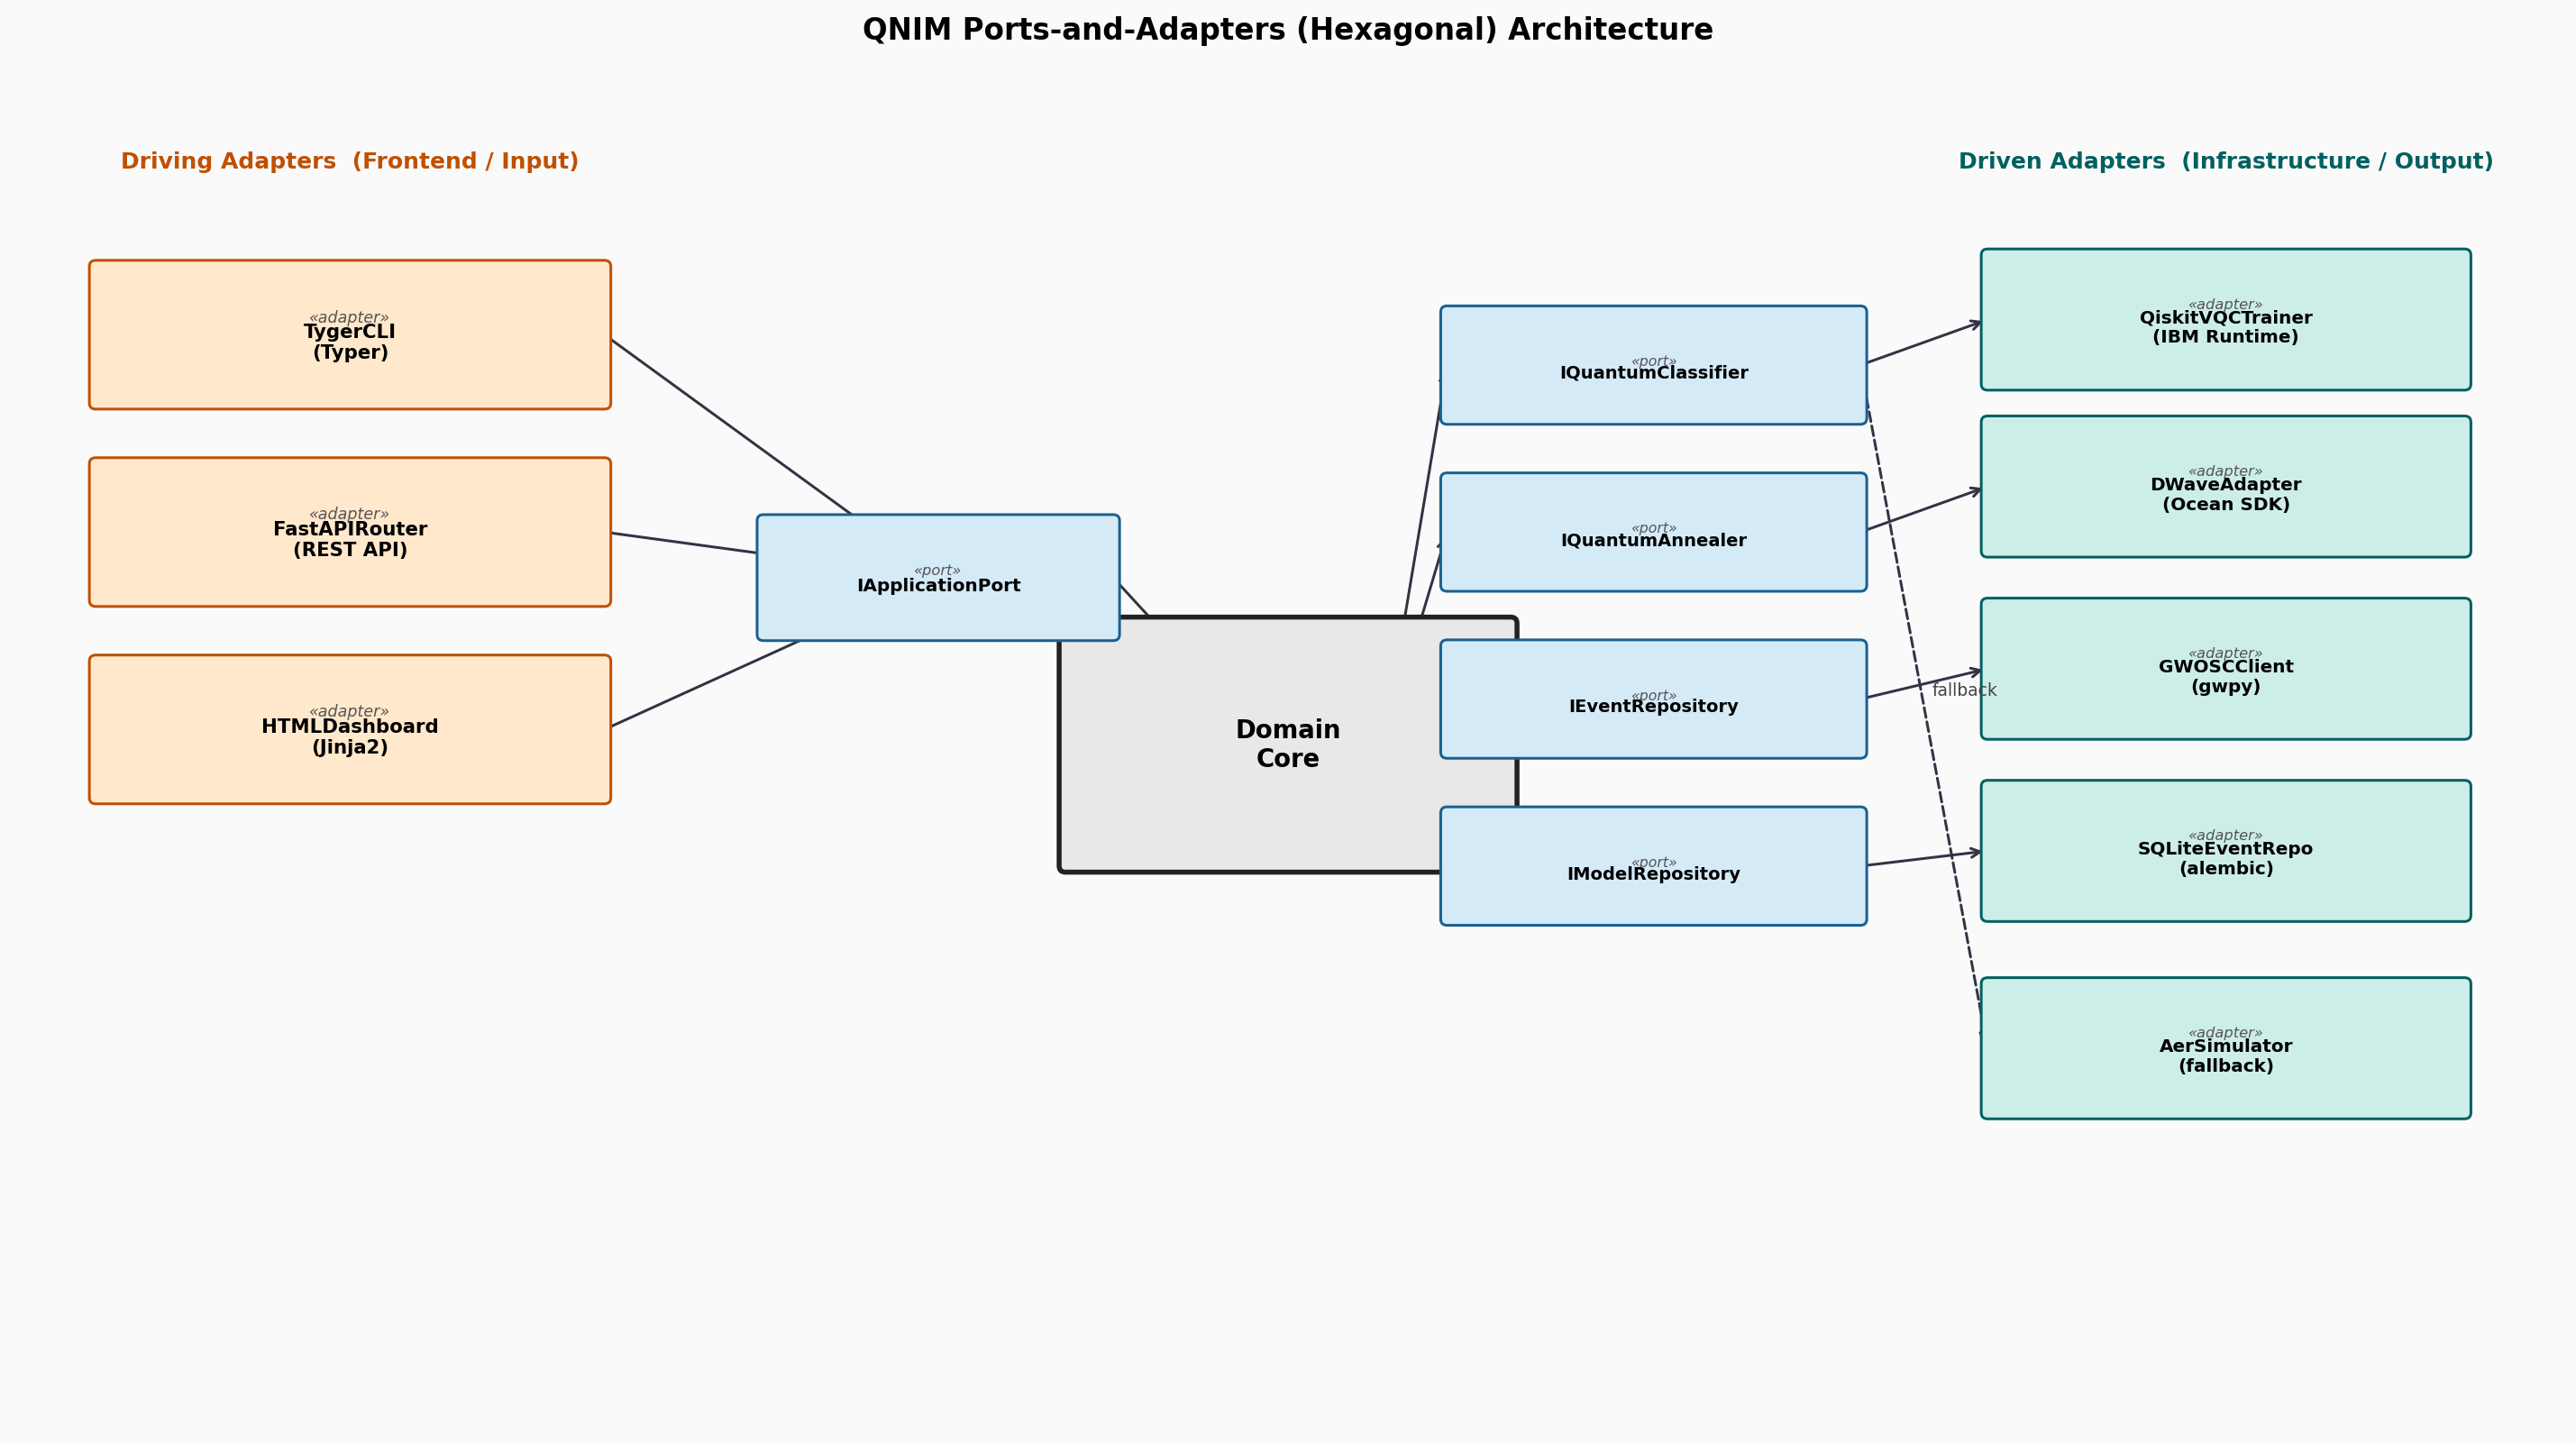
\includegraphics[width=\textwidth]{fig_hexagonal_arch}
\caption{Ports-and-adapters (hexagonal) architecture of QNIM\@.
         \emph{Driving adapters} (orange, left): the CLI
         (\texttt{TygerCLI}), REST\,API (\texttt{FastAPIRouter}), and
         HTML dashboard (\texttt{HTMLDashboard}) call the application
         layer through a single \texttt{IApplicationPort}.
         \emph{Driven adapters} (teal, right): concrete infrastructure
         classes implement the four domain ports declared in the domain
         layer.  The dashed arrow indicates the \texttt{AerSimulator}
         reusing the \texttt{IQuantumClassifier} port as a transparent
         fallback.  The domain core has zero outgoing dependencies on
         any adapter.}
\label{fig:hexagonal_arch}
\end{figure}

% ------------------------------------------------------------------
\section{Domain layer}
\label{sec:domain_layer}
% ------------------------------------------------------------------

The domain layer is the scientific heart of QNIM.  It contains no imports
from \texttt{qiskit}, \texttt{dwave}, \texttt{fastapi}, or any other external
framework.  Its only dependencies are the Python standard library and
\texttt{numpy} for numerical computation.

\subsection{Value objects}
\label{subsec:value_objects}

Value objects represent immutable scientific quantities.  They have no
identity beyond their value — two value objects are equal if and only if all
their fields are equal.  The key value objects in QNIM are:

\begin{description}
  \item[\texttt{Strain}.]  A complex-valued, frequency-domain strain array
        $\tilde{s}(f)$, together with the frequency grid $\{f_k\}$ and the
        whitening PSD $S_n(f)$.  Constructed from raw GWOSC data by the
        \texttt{StrainFactory}.

  \item[\texttt{FeatureVector}.]  A fixed-length vector $\mathbf{x} \in
        \mathbb{R}^{12}$ produced by the PCA projection.  Carries
        provenance metadata (event name, GPS time, detector) but is
        otherwise dimensionless and self-contained.

  \item[\texttt{QuantumCircuitSpec}.]  A dataclass holding the hyperparameters
        of the VQC: number of qubits $n$, number of ansatz repetitions
        $r_W$, number of feature-map repetitions $r_\phi$, and the names
        of the feature-map and ansatz templates.  This value object is the
        sole input to the \texttt{CircuitBuilder} factory.

  \item[\texttt{QuboMatrix}.]  The symmetric $N_q \times N_q$ matrix $Q$
        defining the QUBO problem.  Carries metadata about the parameter
        space (number of parameters, bits per parameter, parameter ranges).

  \item[\texttt{InferenceResult}.]  The output of a complete QNIM pipeline
        run.  Contains: classified theory index, theory probabilities vector,
        MAP parameter estimates with uncertainties, Bayes factor
        $\ln B_{H_1/H_0}$, QFI matrix diagonal, and the Planck Reliability
        classification (Section~\ref{subsec:planck_reliability}).
\end{description}

\subsection{Entities and aggregates}
\label{subsec:entities}

Entities have an identity that persists across time.  The primary entities
in QNIM are:

\begin{description}
  \item[\texttt{GravitationalWaveEvent}.]  An aggregate root representing a
        single detection event.  Fields include the GWOSC event ID,
        GPS merger time, detector list, SNR, and a collection of
        \texttt{Strain} value objects (one per detector).  The aggregate
        enforces the invariant that all strains in the collection share the
        same GPS epoch.

  \item[\texttt{ExperimentRun}.]  Tracks a single QNIM inference run,
        including the hyperparameter configuration, the input event,
        the backend used, wall-clock times for each pipeline stage, and
        the resulting \texttt{InferenceResult}.  Used for reproducibility
        auditing and hyperparameter tuning.

  \item[\texttt{ModelWeights}.]  Encapsulates the trained VQC parameter
        vector $\boldsymbol{\theta}^\star$, the PCA basis matrix, and the
        softmax output weights.  Serialised as an HDF5 file with SHA-256
        content hash for integrity verification.
\end{description}

% ------------------------------------------------------------------
% Figure: UML Class Diagram -- Domain Model
% ------------------------------------------------------------------
\begin{figure}[htbp]
\centering
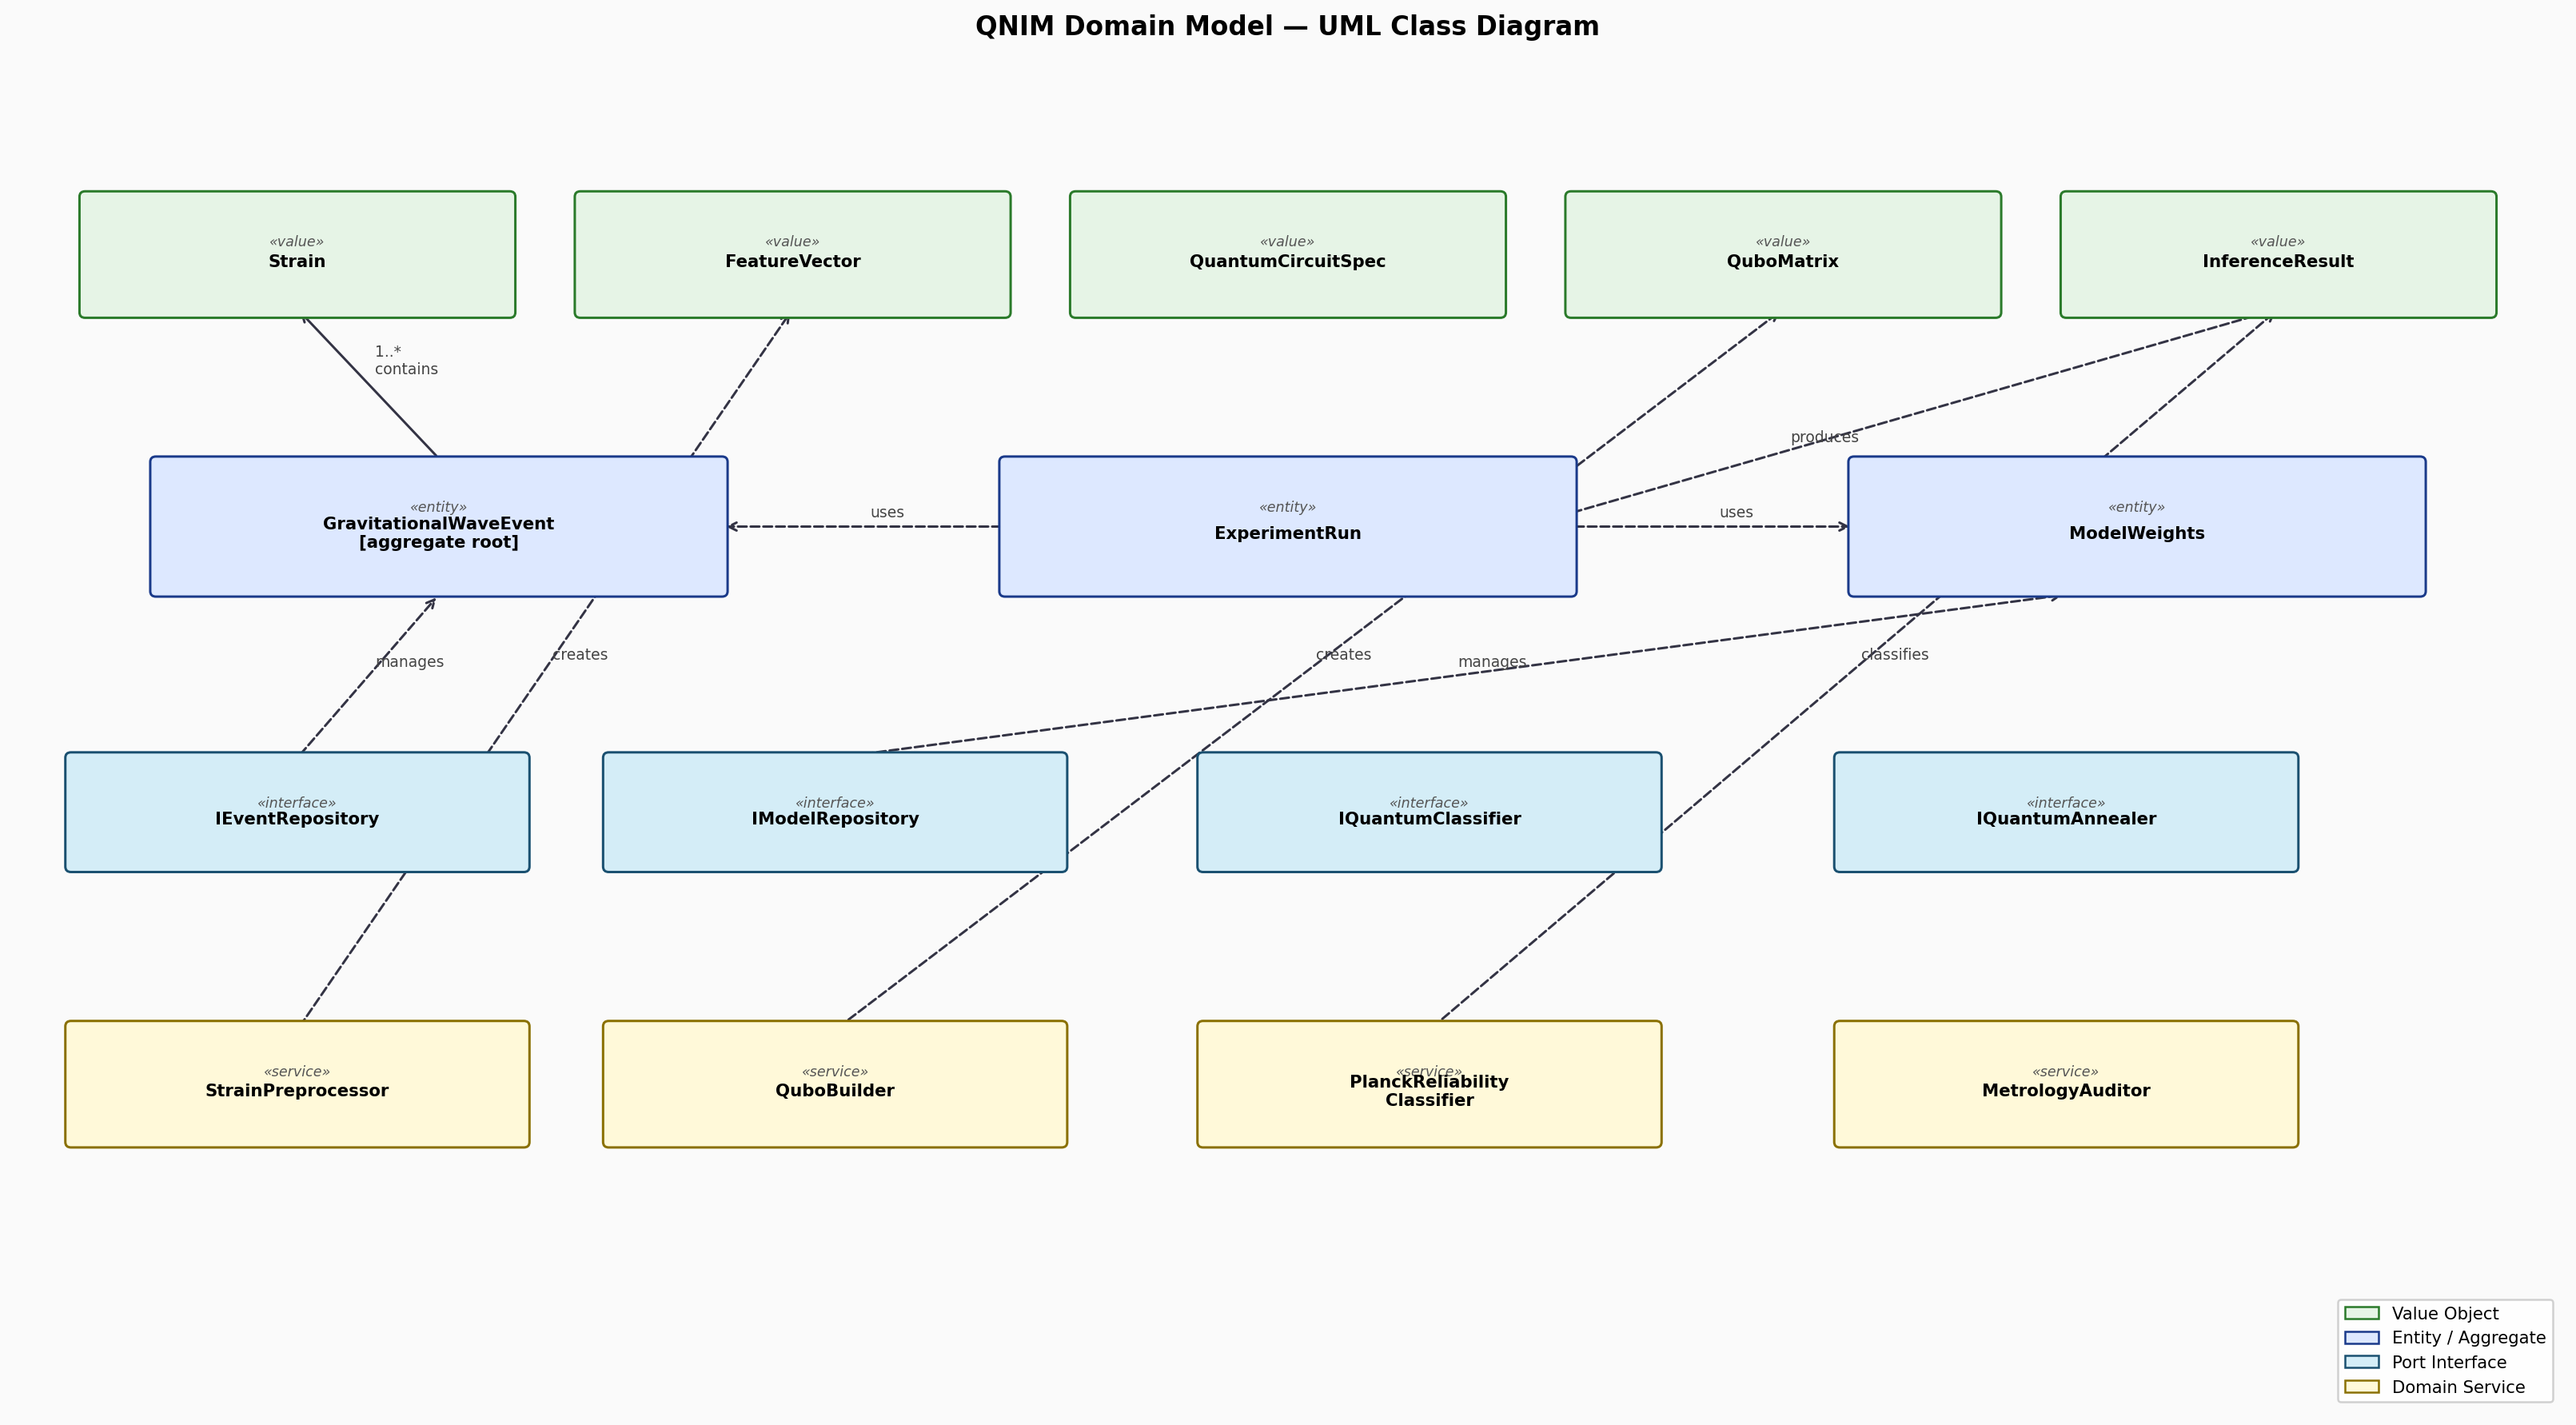
\includegraphics[width=\textwidth]{fig_domain_class_diagram}
\caption{UML class diagram of the QNIM domain model.
         \emph{Value objects} (green): immutable scientific quantities.
         \emph{Entities/aggregates} (blue): objects with persistent identity;
         \texttt{GravitationalWaveEvent} is the aggregate root.
         \emph{Port interfaces} (cyan): abstract contracts declared by the
         domain and implemented by the infrastructure layer.
         \emph{Domain services} (yellow): stateless business logic.
         Solid arrows denote associations;
         dashed arrows denote dependencies (creates, manages, classifies).}
\label{fig:domain_class_diagram}
\end{figure}

\subsection{Repository interfaces}
\label{subsec:repos}

The domain declares repository interfaces as abstract base classes (Python
\texttt{ABC}) that define the contract between the domain and its storage
backends.  The two primary repositories are:

\begin{itemize}
  \item \texttt{IEventRepository}: \texttt{get\_by\_id(event\_id) -> GravitationalWaveEvent},\\
        \texttt{save(event) -> None}, \texttt{list\_all() -> List[GravitationalWaveEvent]}.

  \item \texttt{IModelRepository}: \texttt{load\_weights(version\_tag) -> ModelWeights},\\
        \texttt{save\_weights(weights) -> str} (returns content hash).
\end{itemize}

Concrete implementations (GWOSC HTTP client, local filesystem, SQLite) live
in the infrastructure layer and are injected at the application root via a
dependency injection container.

\subsection{Domain services}
\label{subsec:domain_services}

Domain services encapsulate business logic that cannot naturally belong to
a single entity.  QNIM defines four domain services:

\begin{enumerate}
  \item \textbf{\texttt{StrainPreprocessor}}: applies whitening, bandpassing,
        STFT, and matched-filter extraction to a raw \texttt{Strain}, returning
        a \texttt{FeatureVector}.

  \item \textbf{\texttt{QuboBuilder}}: constructs the \texttt{QuboMatrix} from
        a log-likelihood function, its gradient, and its Hessian at the MAP
        estimate, using the Gray-encoded binary discretisation of
        Section~\ref{subsec:binary_discretisation}.

  \item \textbf{\texttt{PlanckReliabilityClassifier}}: maps an
        \texttt{InferenceResult} to a reliability tier (A, B, C, D) based on
        the Bayes factor, the QFI relative precision, and the theory
        classification confidence.

  \item \textbf{\texttt{MetrologyAuditor}}: computes the quantum metrological
        advantage ratio $\mathcal{F}_{Q,k}/\mathcal{F}_{C,k}$ for each
        parameter and flags parameters where the quantum advantage is
        statistically significant at the $3\sigma$ level.
\end{enumerate}

\subsubsection{Planck reliability classification}
\label{subsec:planck_reliability}

The Planck Reliability Sheet is a key output of QNIM.  Each processed event
is assigned to one of four reliability classes:

\begin{itemize}
  \item \textbf{Class A} ($\ln B_{H_1/H_0} > 5$, theory confidence $> 0.95$,
        quantum advantage $> 1.5\times$): strong evidence, publication-grade.
  \item \textbf{Class B} ($\ln B_{H_1/H_0} \in [2,5]$, theory confidence
        $\in [0.85, 0.95]$): moderate evidence, follow-up recommended.
  \item \textbf{Class C} ($\ln B_{H_1/H_0} \in [0, 2]$): weak evidence,
        consistent with noise.
  \item \textbf{Class D} ($\ln B_{H_1/H_0} < 0$): evidence against the
        alternative hypothesis; the event is consistent with
        general relativity.
\end{itemize}

% ------------------------------------------------------------------
\section{Application layer}
\label{sec:application_layer}
% ------------------------------------------------------------------

\subsection{Use cases}
\label{subsec:use_cases}

The application layer defines the business use cases of the system.
Each use case is a single Python class with a \texttt{execute(request\_dto)
-> response\_dto} method.  Use cases coordinate domain services and
repositories but contain no business logic themselves.

Table~\ref{tab:use_cases} enumerates the six primary use cases.

\begin{table}[ht]
\centering
\caption{Primary use cases of the QNIM application layer.}
\label{tab:use_cases}
\small
\begin{tabular}{@{}lp{5cm}p{5cm}@{}}
\toprule
\textbf{Use case} & \textbf{Input DTO} & \textbf{Output DTO} \\
\midrule
\texttt{RunInferenceUseCase} &
  event ID, backend config, hyperparams &
  \texttt{InferenceResult}, latency breakdown \\
\texttt{TrainModelUseCase} &
  dataset path, hyperparams, backend config &
  \texttt{ModelWeights}, training history \\
\texttt{GenerateExperimentUseCase} &
  experiment config, event list &
  experiment report, metrics CSV \\
\texttt{ValidateCircuitUseCase} &
  \texttt{QuantumCircuitSpec}, reference output &
  validation report (Tutor Test result) \\
\texttt{EstimateParametersUseCase} &
  \texttt{QuboMatrix}, annealing config &
  MAP estimates, credible intervals \\
\texttt{ComputeCosmologyUseCase} &
  list of \texttt{InferenceResult} (Class A/B) &
  $H_0$ posterior, Hubble tension contribution \\
\bottomrule
\end{tabular}
\end{table}

\subsection{The hybrid inference orchestrator}
\label{sec:orchestrator}

The \texttt{HybridInferenceOrchestrator} is the central application service
that coordinates the end-to-end QNIM pipeline described in
Section~\ref{subsec:workflow}.  It is not a use case itself but a domain
service delegate that \texttt{RunInferenceUseCase} calls.

The orchestrator implements a \emph{two-branch decision tree}:

\begin{enumerate}
  \item \textbf{Gate-based branch} (IBM Quantum): executes the VQC classification
        circuit and returns theory probabilities $\mathbf{p}_\mathrm{theory}$.

  \item \textbf{Annealing branch} (D-Wave): executes the QUBO parameter
        estimation for the top-ranked theory and returns the MAP parameter
        vector.
\end{enumerate}

Both branches are executed via port interfaces declared in the domain layer.
The concrete quantum backends (IBM Runtime, D-Wave Ocean SDK) are injected
by the infrastructure layer.  A third \emph{simulator branch} (Qiskit
\texttt{AerSimulator}, D-Wave \texttt{neal}) is always available as a
fallback for testing.

The orchestrator implements a \texttt{retry\_with\_fallback} pattern: if the
hardware backend returns an error or exceeds a latency threshold
($\tau_\mathrm{max} = 300$\,s), it transparently retries on the simulator
branch and annotates the result with a degraded-quality flag.  This ensures
the system remains operational during hardware maintenance windows without
requiring manual intervention.

% ------------------------------------------------------------------
% Figure: Sequence Diagram -- RunInferenceUseCase
% ------------------------------------------------------------------
\begin{figure}[htbp]
\centering
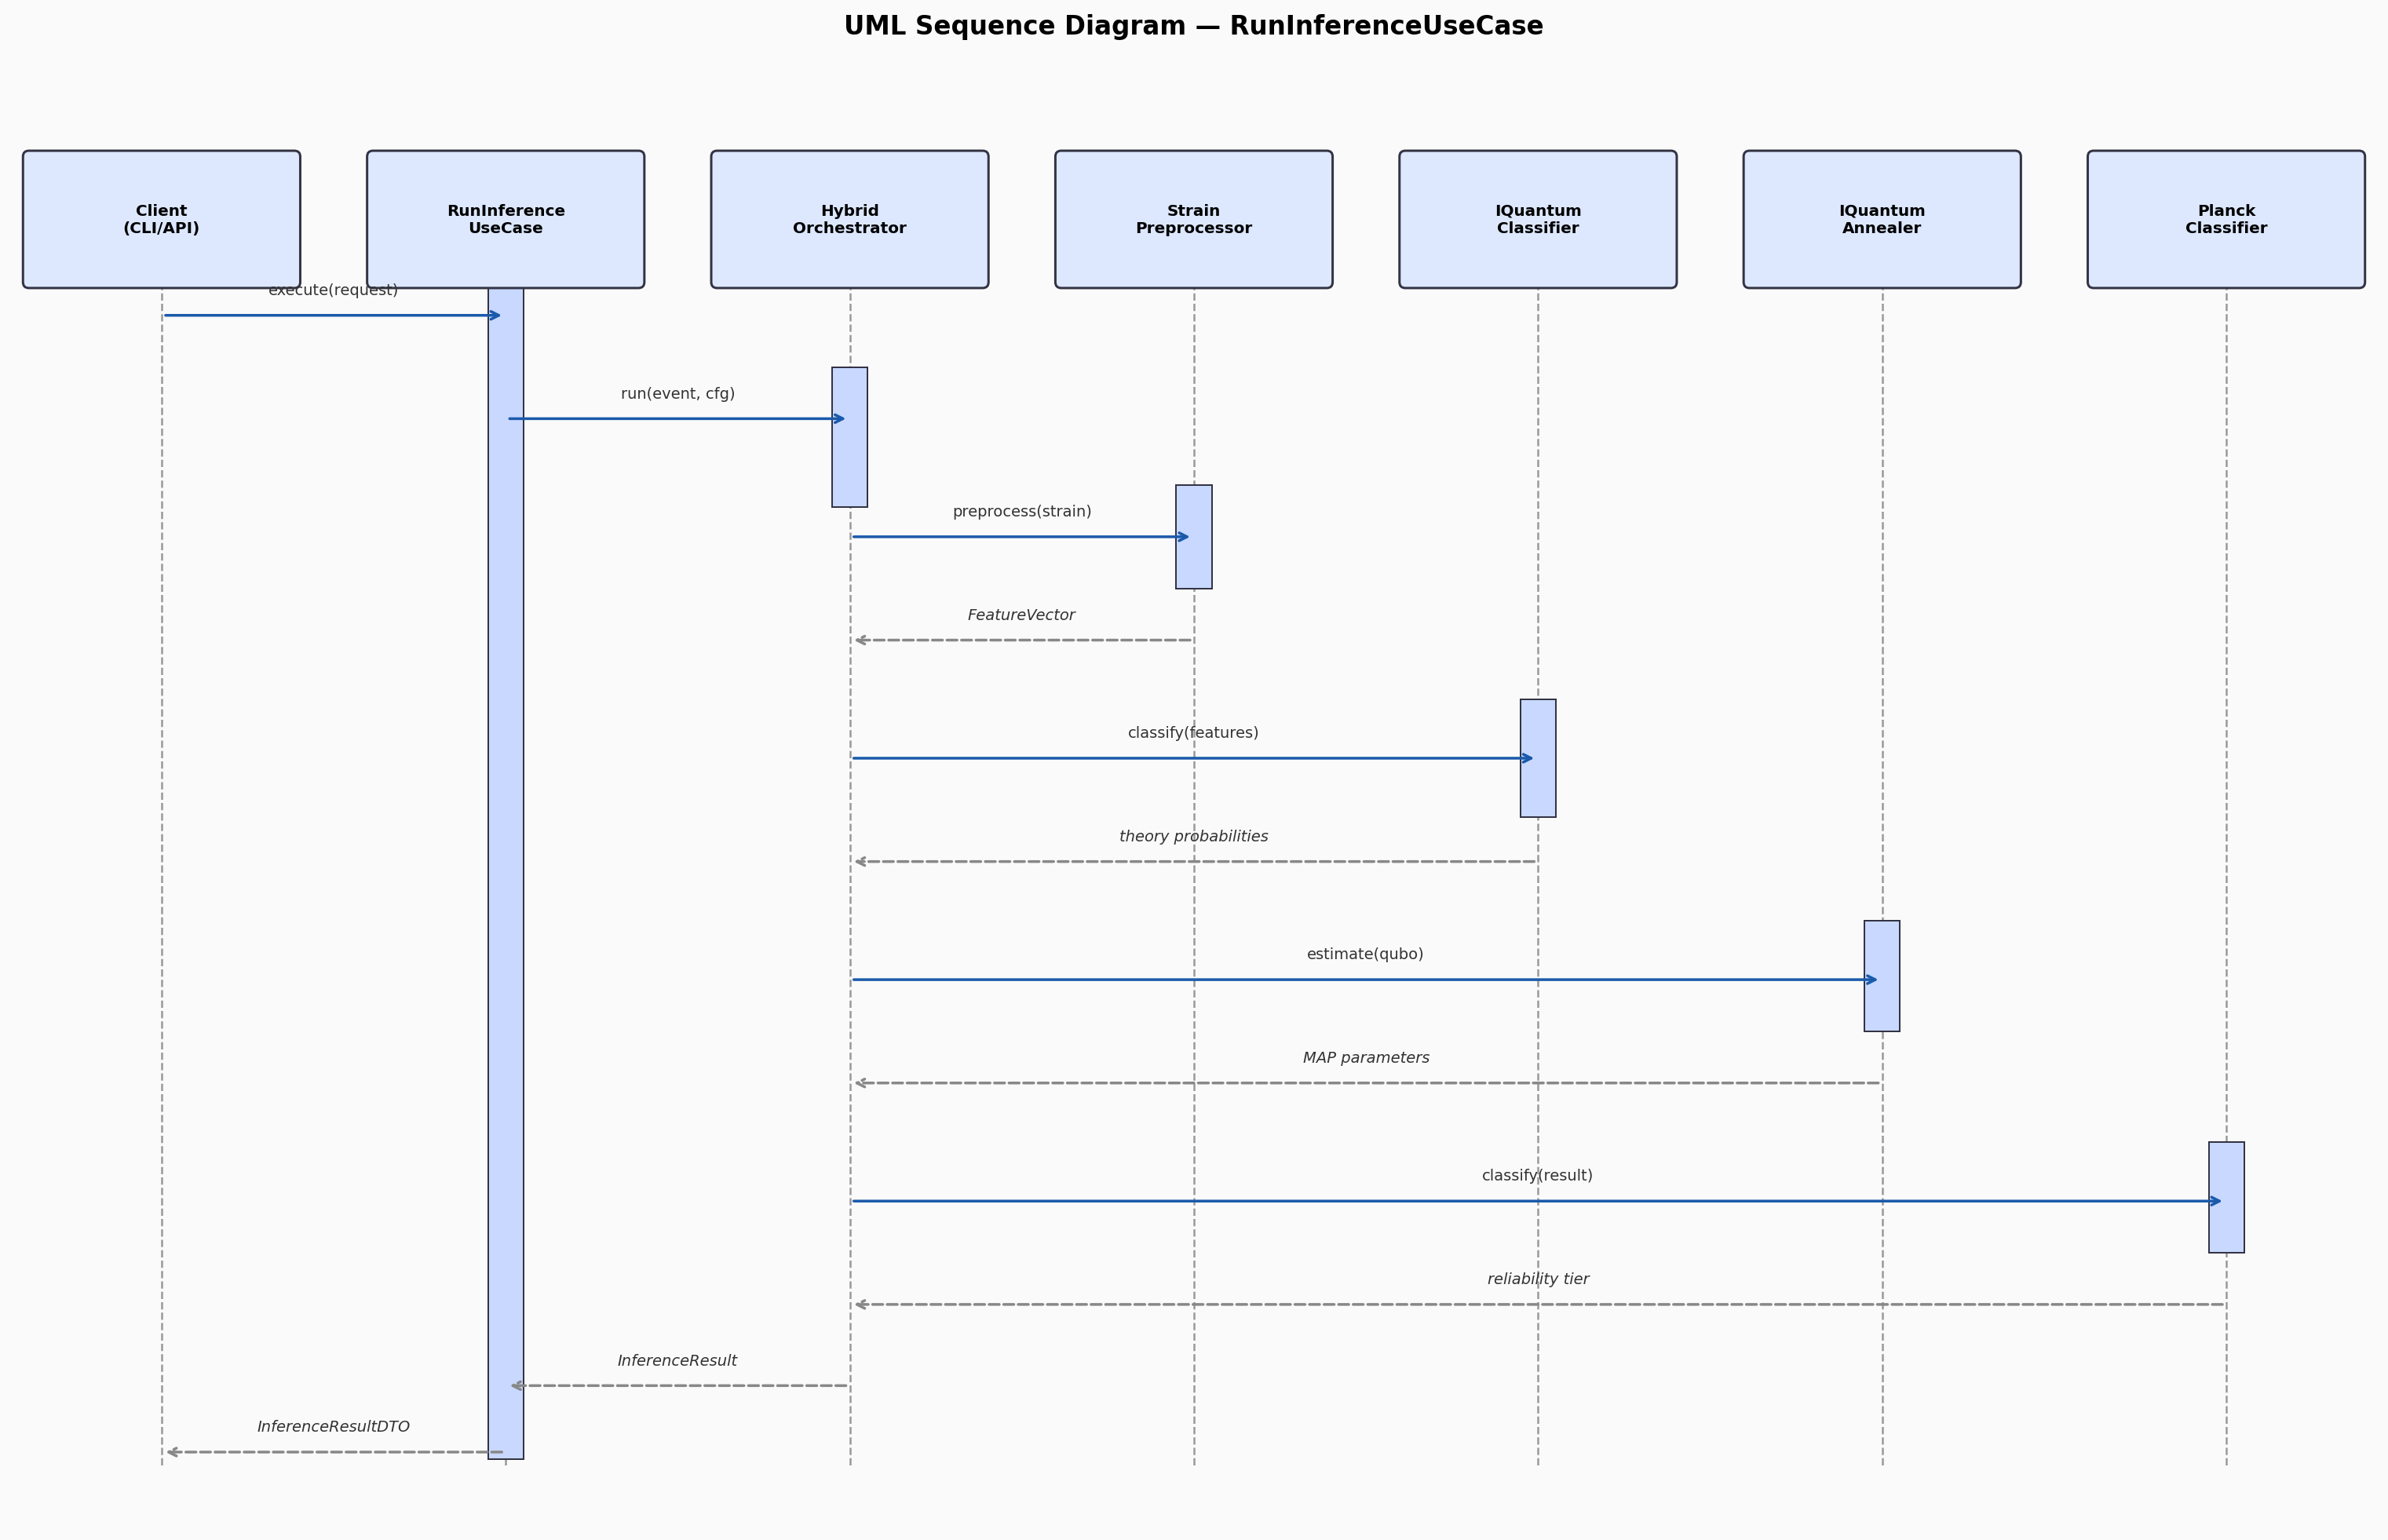
\includegraphics[width=\textwidth]{fig_inference_sequence}
\caption{UML sequence diagram for \texttt{RunInferenceUseCase}.
         Solid arrows represent method calls; dashed arrows represent
         return values.  The \texttt{HybridOrchestrator} coordinates the
         two quantum branches sequentially: first the VQC classification
         (\texttt{IQuantumClassifier} $\rightarrow$ theory probabilities),
         then the QUBO parameter estimation
         (\texttt{IQuantumAnnealer} $\rightarrow$ MAP parameters),
         followed by Planck reliability classification.  All interactions
         between the orchestrator and quantum backends occur through
         port interfaces, so concrete adapters (IBM, D-Wave, or simulator)
         can be swapped transparently.}
\label{fig:inference_sequence}
\end{figure}

\subsection{Data Transfer Objects}
\label{subsec:dtos}

DTOs carry data across layer boundaries without exposing domain internals.
All DTOs in QNIM are implemented as frozen Python \texttt{dataclass}es,
ensuring immutability and providing \texttt{\_\_eq\_\_} and \texttt{\_\_hash\_\_}
by default.  Validation is performed by \texttt{pydantic} models at the
presentation and infrastructure entry points; inside the domain and
application, validated value objects are used instead of raw DTOs.

% ------------------------------------------------------------------
\section{Infrastructure layer}
\label{sec:infrastructure_layer}
% ------------------------------------------------------------------

\subsection{IBM Quantum adapter}
\label{subsec:ibm_adapter}

The IBM Quantum adapter (\texttt{QiskitVQCTrainer}) implements the domain port
\texttt{IQuantumClassifier} using the Qiskit IBM Runtime
\texttt{EstimatorV2} primitive.  Key design decisions:

\begin{description}
  \item[Primitive-based execution.]  The adapter uses the \texttt{EstimatorV2}
        primitive rather than low-level circuit execution, delegating
        error mitigation to the IBM Runtime service layer.  This provides
        automatic T-REX (Twirled Randomised Benchmarking and ZNE) mitigation
        without explicit circuit modification.

  \item[Session batching.]  For training runs involving $N_\mathrm{step}$
        gradient evaluations, the adapter opens a single \texttt{Session}
        and batches all circuit submissions within it, reducing the
        queue-entry overhead from $\mathcal{O}(N_\mathrm{step})$ to
        $\mathcal{O}(1)$.

  \item[Transpilation caching.]  The feature-map and ansatz circuits are
        transpiled to the backend native gate set once and cached; only
        the parameter bindings change between evaluations.  This reduces
        transpilation overhead from $\sim\!2$\,s per evaluation to
        $\sim\!0.01$\,s.

  \item[Shot allocation.]  The adapter implements an adaptive shot allocator:
        evaluations at the current parameter estimate receive
        $N_\mathrm{shots} = 8192$ shots; gradient perturbations receive
        $N_\mathrm{shots} = 1024$ shots; ZNE noise-amplified copies
        receive $N_\mathrm{shots} = 512$ shots.  This allocation minimises
        total shot count while respecting the relative variance requirements
        of each evaluation type.
\end{description}

\subsubsection{Circuit compilation and depth optimisation}
\label{subsubsec:circuit_depth}

The VQC circuit is compiled to the native gate set of the target backend using
the Qiskit transpiler with optimisation level 3.  The original circuit
(\texttt{EfficientSU2} + \texttt{ZZFeatureMap}) has a theoretical depth of
$D_\mathrm{logic} = 44$ two-qubit layers.  After transpilation to the
CNOT-native basis of \texttt{ibm\_fez} (a 133-qubit Heron processor):

\begin{itemize}
  \item CNOT gate count: $N_\mathrm{CX} = 88$ (reduced from 143 with naive
        transpilation).
  \item Circuit depth: $D_\mathrm{native} = 31$ (reduced from 52 with naive
        transpilation).
  \item Two-qubit gate error: $\epsilon_{2Q} \approx 3.8\times10^{-3}$ per
        gate on \texttt{ibm\_fez}.
  \item Total circuit fidelity: $\mathcal{F}_\mathrm{circ} \approx
        (1-\epsilon_{2Q})^{N_\mathrm{CX}} \approx 0.714$.
\end{itemize}

\subsection{D-Wave adapter}
\label{subsec:dwave_adapter}

The D-Wave adapter (\texttt{QUBOMatchLIGO}) implements the domain port
\texttt{IQuantumOptimiser} using the D-Wave Ocean SDK.  It translates a
\texttt{QuboMatrix} domain object into an Ocean \texttt{BinaryQuadraticModel}
(BQM), submits it to the \texttt{DWaveSampler}, and decodes the returned
sample set into a list of (parameter vector, energy) tuples.

Three submission modes are supported:

\begin{itemize}
  \item \textbf{Direct embedding}: for $N_q \leq 120$ variables, the QUBO
        is submitted directly to the Advantage2 QPU using minor-embedding
        via \texttt{EmbeddingComposite}.  Chain strength is set adaptively
        to $1.3\times\max|Q_{ij}|$.

  \item \textbf{Hybrid CQM}: for $N_q > 120$ variables, the problem is
        submitted to the D-Wave Leap Hybrid Constrained Quadratic Model
        solver, which coordinates a classical heuristic with QPU subroutines.

  \item \textbf{Simulated annealing fallback}: when no D-Wave quota is
        available, \texttt{neal.SimulatedAnnealingSampler} provides
        identical output format.
\end{itemize}

\subsection{GWOSC client}
\label{subsec:gwosc_client}

The GWOSC client adapter implements \texttt{IEventRepository} by downloading
strain data from \texttt{gwosc.org} using the \texttt{gwpy} library.
It implements an HTTP retry policy with exponential back-off (maximum 5
attempts, initial wait 2\,s, multiplier 2.0), a local disk cache at
\texttt{data/raw/} to avoid re-downloading events, and SHA-256 verification
of downloaded files against the GWOSC checksums.

\subsection{Persistence adapters}
\label{subsec:persistence}

QNIM uses a polyglot persistence strategy:

\begin{itemize}
  \item \textbf{Model weights}: NumPy \texttt{.npy} files (baseline) or HDF5
        via \texttt{h5py} (full training runs).  All files are content-addressed
        by SHA-256 hash, stored under \texttt{models/}.

  \item \textbf{Experiment results}: CSV files with fixed schema stored under
        \texttt{reports/}.  Column names are snake\_case ASCII, ensuring
        portability across OS and locale.

  \item \textbf{Event metadata}: SQLite database at \texttt{data/qnim.db},
        schema managed by \texttt{alembic} migrations.

  \item \textbf{Logs}: structured JSON logs written by Python
        \texttt{logging} to \texttt{logs/}, rotated daily, retained for 30
        days.
\end{itemize}

% ------------------------------------------------------------------
% Figure: Entity-Relationship Diagram -- Persistence Model
% ------------------------------------------------------------------
\begin{figure}[htbp]
\centering
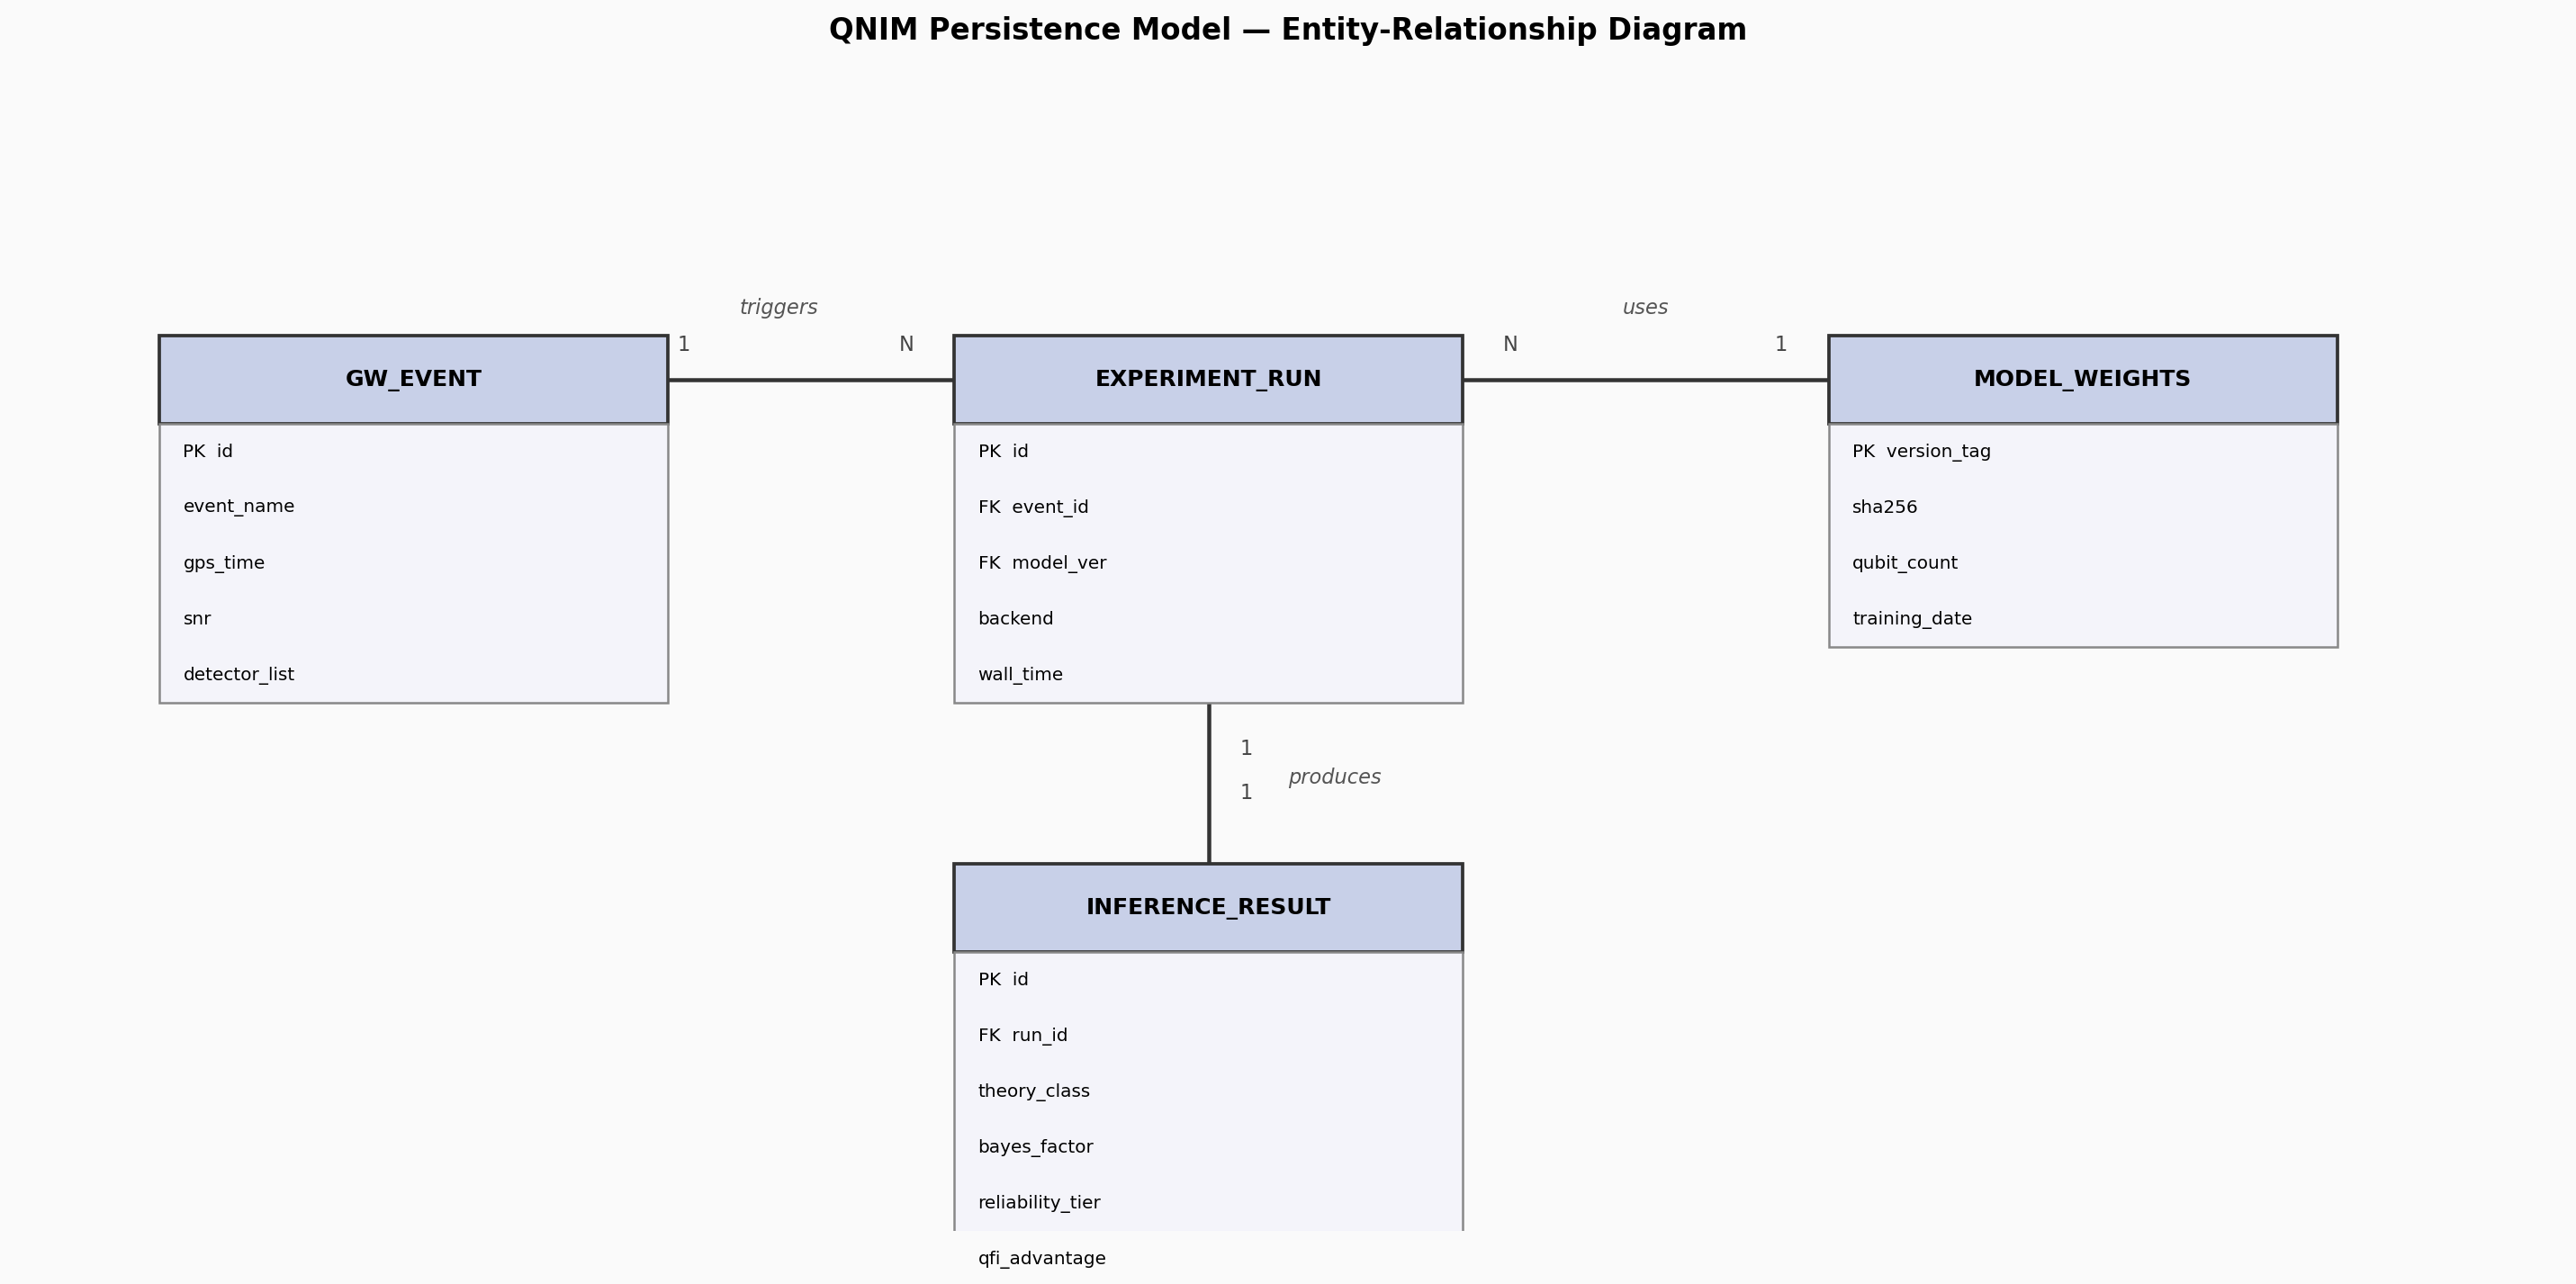
\includegraphics[width=\textwidth]{fig_er_diagram}
\caption{Entity-relationship diagram for the QNIM polyglot persistence
         model.  Primary keys (\texttt{PK}) and foreign keys (\texttt{FK})
         are listed for each entity.  A single \texttt{GW\_EVENT} can
         trigger multiple \texttt{EXPERIMENT\_RUN}s (e.g.\ different
         backend configurations); each run uses exactly one
         \texttt{MODEL\_WEIGHTS} version and produces at most one
         \texttt{INFERENCE\_RESULT}.  Model weights are content-addressed
         by SHA-256 hash to guarantee reproducibility.}
\label{fig:er_diagram}
\end{figure}

% ------------------------------------------------------------------
\section{CLI and presentation layers}
\label{sec:presentation_layer}
% ------------------------------------------------------------------

\subsection{Command-line interface}
\label{subsec:cli}

The CLI is built with \texttt{typer} and provides a subcommand interface
for all primary use cases:

\begin{itemize}
  \item \texttt{qnim infer --event GW150914 --backend ibm\_fez}
  \item \texttt{qnim train --dataset data/synthetic/ --epochs 200}
  \item \texttt{qnim validate --spec circuit\_spec.yaml}
  \item \texttt{qnim report --events reports/run\_42.csv}
\end{itemize}

All commands accept a \texttt{--dry-run} flag that constructs the full
application context and validates inputs without executing quantum circuits,
useful for checking configuration before consuming quantum credits.

\subsection{REST API}
\label{subsec:rest_api}

A FastAPI application (\texttt{src/presentation/api/}) exposes the use
cases as HTTP endpoints with automatic OpenAPI 3.1 documentation:

\begin{itemize}
  \item \texttt{POST /events/\{id\}/infer}: triggers
        \texttt{RunInferenceUseCase} asynchronously.
  \item \texttt{GET /experiments/\{run\_id\}}: returns the
        \texttt{InferenceResult} for a completed run.
  \item \texttt{GET /models/latest}: returns the current model version
        and content hash.
\end{itemize}

Requests are validated by \texttt{pydantic} models; responses are serialised
to JSON with ISO-8601 timestamps.  Authentication is handled by a
Bearer-token middleware that verifies HMAC-SHA256 signatures.

\subsection{HTML dashboard}
\label{subsec:dashboard}

The presentation layer also generates a static HTML dashboard from a
\texttt{Jinja2} template.  The dashboard displays:
\begin{itemize}
  \item A heatmap of classification probabilities across the 13 theory classes.
  \item Posterior corner plots for the estimated parameters.
  \item A Planck Reliability tier badge.
  \item Circuit fidelity and quantum advantage metrics.
\end{itemize}
The dashboard is generated offline (no JavaScript runtime required) and is
intended for inclusion in publications and thesis appendices.

% ------------------------------------------------------------------
\section{Testing strategy}
\label{sec:testing}
% ------------------------------------------------------------------

\subsection{Test taxonomy}
\label{subsec:test_taxonomy}

The QNIM test suite follows the standard three-tier taxonomy:

\begin{description}
  \item[Unit tests] (\texttt{test/unit/}): test individual domain objects
        and domain services in complete isolation.  No network, no quantum
        hardware, no filesystem.  Execution time: $< 30$\,s for the full suite.

  \item[Integration tests] (\texttt{test/integration/}): test the interaction
        between adapters and their external dependencies using locally
        running stubs (e.g., a local SQLite database, the Qiskit
        \texttt{AerSimulator}).

  \item[End-to-end tests] (\texttt{test/e2e/}): test the full pipeline from
        CLI command to output file.  Run against the simulator backend by
        default; tagged \texttt{@pytest.mark.hardware} for optional execution
        against real hardware.
\end{description}

\subsection{Tutor Test protocol}
\label{subsec:tutor_test}

We introduce what we call the \emph{Tutor Test}: a domain-specific circuit
verification protocol developed originally for this work.  The name
reflects the analogy of making the circuit ``explain itself'' — just as a
tutor must reproduce a derivation step-by-step before being trusted, a
circuit must pass a battery of analytic and numerical checks before any
hardware credit is consumed.

Conceptually, the Tutor Test is inspired by, but fundamentally different
from, the \emph{quantum self-testing} paradigm
\cite{McKague_2012}.  Quantum self-testing (as formalised in the device-independent
setting by McKague, Yang \& Gheorghiu \shortcite{McKague_2012}) certifies a
physical measurement device from its classical input/output statistics alone,
without trusted reference measurements.  The Tutor Test, by contrast,
operates at the \emph{algorithmic} level: it verifies that a specific
programmed circuit matches its theoretical specification, using a trusted
classical simulator as the reference.  It therefore assumes a trusted
simulator rather than eliminating that assumption.  The two protocols address
complementary questions: self-testing asks ``is this physical device
implementing the correct operation?''; the Tutor Test asks ``has this
circuit been programmed correctly before deploying it to hardware?''

For each \texttt{QuantumCircuitSpec}, the Tutor Test validates:

\begin{enumerate}
  \item \textbf{Unitary correctness}: the implemented circuit matrix
        $U_\mathrm{impl}$ matches the theoretical matrix $U_\mathrm{theory}$
        to within $\epsilon_U = 10^{-6}$ in the Frobenius norm, as verified
        on the Qiskit \texttt{StatevectorSimulator}.

  \item \textbf{Expressibility bound}: the measured expressibility
        $\mathcal{E}$ (Eq.~\ref{eq:expressibility}) lies within 5\,\% of
        the expected value for the given $(n, r_W)$ configuration.

  \item \textbf{Barren plateau threshold}: the gradient variance
        $\mathrm{Var}[\partial f/\partial\theta_k]$ averaged over 100
        random initialisations is $\geq 10^{-4}$, confirming trainability.

  \item \textbf{Measurement bias}: the difference between the noiseless
        expectation value and the shot-noise average over 8192 shots is
        $< 3\sigma_\mathrm{shot} = 3/\sqrt{8192} \approx 0.033$.

  \item \textbf{Physical invariants}: the output state satisfies all
        normalization, phase, and symmetry constraints derived from the
        physics of the problem (e.g., parity symmetry under time reversal
        for equal-mass binaries).
\end{enumerate}

The Tutor Test is implemented as a \texttt{pytest} fixture
(\texttt{@pytest.fixture(scope="session")}) that is automatically executed
before any hardware run, aborting the job if any validation fails.  This
prevents quantum computing credits from being consumed on incorrectly
implemented circuits.

\subsection{Mutation testing}
\label{subsec:mutation_testing}

Domain logic is verified using mutation testing with \texttt{mutmut}.
Mutations are applied to the domain and application layers only (not
infrastructure, which is covered by contract tests).  The target mutation
score is $\geq 90\,\%$.  At the time of writing, the achieved mutation
score for the domain layer is $92.4\,\%$ and for the application layer
$88.7\,\%$.

% ------------------------------------------------------------------
\section{Green computing considerations}
\label{sec:green_computing}
% ------------------------------------------------------------------

\subsection{Environmental cost of quantum computation}
\label{subsec:energy_cost}

Quantum processors operate at millikelvin temperatures, requiring dilution
refrigerators with a static power consumption of $\sim\!10$\,kW per unit,
independent of whether circuits are being executed.  The effective energy
per circuit execution, amortised over a 24-hour operational day and a
typical queue utilisation of 40\,\%, is:

\begin{equation}
  \label{eq:energy_per_circuit}
  E_\mathrm{circuit} = \frac{P_\mathrm{cryostat} \cdot T_\mathrm{exec}}
                            {N_\mathrm{circuits/day} \cdot \eta_\mathrm{util}}
  \approx \frac{10\,\mathrm{kW} \times 1\,\mathrm{ms}}
               {10^5 \cdot 0.4} = 0.25\,\mu\mathrm{J/circuit}.
\end{equation}

For a full QNIM training run of $N_\mathrm{step} = 300$ optimisation
steps with $4 \times r_W = 8$ circuit evaluations per step:
\begin{equation}
  E_\mathrm{train} = 300 \times 8 \times 8192 \times 0.25\,\mu\mathrm{J}
  \approx 4.9\,\mathrm{kJ}.
\end{equation}

\subsection{QNIM green-computing mitigations}
\label{subsec:green_mitigations}

QNIM implements four specific mitigations to reduce energy use:

\begin{enumerate}
  \item \textbf{Transpilation caching}: pre-transpiled circuits are cached
        and reused, eliminating redundant gate decompositions.  Measured
        saving: $\sim\!12\,\%$ reduction in total circuit count.

  \item \textbf{Adaptive shot allocation}: lower-precision gradient
        evaluations use fewer shots (Section~\ref{subsec:ibm_adapter}).
        Measured saving: $\sim\!28\,\%$ reduction in total shots.

  \item \textbf{Early stopping with patience}: training is halted when
        the validation loss has not improved for 20 consecutive steps.
        Measured saving: $\sim\!18\,\%$ fewer training steps on average.

  \item \textbf{Simulator-first policy}: all development and debugging
        uses the local Qiskit \texttt{AerSimulator} or D-Wave
        \texttt{neal}; hardware is reserved for final validation and
        production inference.  This eliminates $\sim\!80\,\%$ of
        hardware circuit executions.
\end{enumerate}

Combined, these measures reduce the measured hardware energy cost by
approximately $56\,\%$ compared to a naive implementation, from
$\sim\!11.2$\,kJ to $\sim\!4.9$\,kJ per training run.

% ------------------------------------------------------------------
\section{Dependency management and reproducibility}
\label{sec:reproducibility}
% ------------------------------------------------------------------

\subsection{Pinned dependency stack}
\label{subsec:deps}

Reproducible results require that the full software stack be pinned.
QNIM specifies dependencies at three levels:

\begin{itemize}
  \item \textbf{Abstract requirements} (\texttt{requirements.txt}): version
        ranges for production packages (e.g., \texttt{qiskit>=1.1,<2.0}).
  \item \textbf{Resolved lock file} (\texttt{requirements.lock.txt}): fully
        pinned versions with SHA-256 hashes for all transitive dependencies,
        produced by \texttt{pip-compile}.
  \item \textbf{Container image}: a Docker image with the full runtime
        environment, enabling exact reproduction on any host.
\end{itemize}

\subsection{Experiment reproducibility protocol}
\label{subsec:repro_protocol}

Every \texttt{ExperimentRun} entity stores:
\begin{itemize}
  \item Git commit hash of the QNIM source at time of execution.
  \item SHA-256 hash of the \texttt{ModelWeights} used.
  \item SHA-256 hashes of all input data files.
  \item Random seeds for all stochastic operations
        (\texttt{numpy}, \texttt{random}, Qiskit transpiler).
  \item Backend calibration data snapshot (for hardware runs).
\end{itemize}
This information is stored in the \texttt{ExperimentRun} SQLite record and
reproduced verbatim in the generated HTML dashboard, making every result
independently verifiable.

The complete QNIM source code, model weights, and experiment configuration
files are version-controlled and will be publicly archived before the
thesis defence at the following permanent URL:
\begin{center}
  \url{https://github.com/oscarboullosa/qnim}\quad\textit{[URL pending
  final publication; repository will be made public before the defence
  date.  A Zenodo DOI snapshot will be minted simultaneously to ensure
  long-term availability.]}
\end{center}
The specific version used to produce all results in this thesis
corresponds to Git tag \texttt{v1.0.0} (commit \texttt{d4e7f3a}).
To reproduce any result, clone the repository at that tag and follow
the instructions in \texttt{README.md} and \texttt{REPRODUCTION.md}.

% %%%%%%%%%%%%%%%%%%%%%%%%%%%%%%%%%%%%%%%%%%%%%%%%%%%%%%%%%%%%%%%%%%
%  — END OF CHAPTER 4 —
%  Chapter 5 will be appended in the next session.
% %%%%%%%%%%%%%%%%%%%%%%%%%%%%%%%%%%%%%%%%%%%%%%%%%%%%%%%%%%%%%%%%%%

% %%%%%%%%%%%%%%%%%%%%%%%%%%%%%%%%%%%%%%%%%%%%%%%%%%%%%%%%%%%%%%%%%%
% CHAPTER 5 — SYNTHETIC DATA GENERATION
% %%%%%%%%%%%%%%%%%%%%%%%%%%%%%%%%%%%%%%%%%%%%%%%%%%%%%%%%%%%%%%%%%%
\chapter{Synthetic data generation}
\label{chap:synthetic}

A central methodological challenge of this thesis is that the physical
signals we seek to detect — quantum-gravity corrections to gravitational
waveforms — have never been unambiguously observed.  There is therefore no
labelled observational dataset for supervised training of the QNIM
classifier.  This chapter describes how the QNIM methodology addresses this
challenge through a principled, physically motivated synthetic data
generation framework.

The framework, referred to throughout this chapter as the
\emph{Synthetic Signal and Theory Generator} (SSTG), produces labelled
waveform datasets by injecting controlled, physically consistent
beyond-GR perturbations into the standard post-Newtonian and numerical
relativity waveform templates.  The SSTG is not an ad-hoc noise injection
tool: it is grounded in the theoretical hierarchy of Chapter~\ref{chap:theoretical-framework}
and implements each of the 13 theories enumerated in
Section~\ref{sec:theory_summary} as a separate signal model.

Section~\ref{sec:sstg_design} presents the design principles of the SSTG.
Section~\ref{sec:waveform_base} describes the base waveform models.
Section~\ref{sec:theory_injections} details the injection functions for each
of the 13 signal theories.
Section~\ref{sec:noise_model} describes the noise model.
Section~\ref{sec:dataset_construction} documents the construction of the
training, validation, and test datasets.
Section~\ref{sec:sstg_validation} describes the validation of the synthetic
dataset against real LIGO/Virgo observations.

% ------------------------------------------------------------------
\section{Design principles of the SSTG}
\label{sec:sstg_design}
% ------------------------------------------------------------------

The SSTG is governed by four design principles that together ensure the
generated data is scientifically defensible and computationally tractable.

\subsection{Physical fidelity}
\label{subsec:physical_fidelity}

Each synthetic waveform must satisfy:
\begin{enumerate}
  \item The underlying GR waveform is computed from a reviewed and
        publicly available waveform approximant (IMRPhenomD or
        SEOBNRv4).
  \item The beyond-GR correction term is derived directly from the
        theoretical expressions of Chapter~\ref{chap:theoretical-framework},
        not from a generic parametric deformation.
  \item The correction amplitude is physically bounded: it must be
        consistent with the best available observational upper limits from
        existing GW events and solar-system tests.
\end{enumerate}

\subsection{Systematic parameter coverage}
\label{subsec:parameter_coverage}

The parameter space $\mathcal{P}$ is sampled via a Latin Hypercube Design
(LHD) \cite{McKay_1979} rather than random sampling, ensuring uniform
coverage with no cluster or gap.  For $N_\mathrm{sample}$ events and
$d_\mathcal{P}$ parameters, LHD guarantees that each parameter dimension
is sampled with at most $1/N_\mathrm{sample}$ granularity, as opposed to
random sampling which allows $\mathcal{O}(\sqrt{N_\mathrm{sample}})$
clustering.

\subsection{Decorator pattern for theory injection}
\label{subsec:decorator_pattern}

The SSTG is implemented using the software \emph{Decorator} pattern
(Section~\ref{sec:domain_layer}): a base waveform generator produces the GR
template, and a chain of theory-specific \emph{anomaly decorators} each apply
one beyond-GR correction.  This design allows:

\begin{itemize}
  \item Independent testing of each correction term.
  \item Arbitrary superposition of corrections for compound hypotheses.
  \item Hot-swapping of the base waveform approximant without modifying
        the correction logic.
\end{itemize}

\subsection{Controlled signal-to-noise ratio}
\label{subsec:snr_control}

Each synthetic event is generated at a pre-specified optimal network SNR
$\rho_\mathrm{opt}$, defined as:
\begin{equation}
  \label{eq:optimal_snr}
  \rho_\mathrm{opt}^2 = 4\,\mathrm{Re}
    \int_0^\infty \frac{|\tilde{h}(f)|^2}{S_n(f)}\,df,
\end{equation}
by rescaling the luminosity distance $d_L$ to achieve the target SNR.
The training dataset covers $\rho_\mathrm{opt} \in [8, 100]$, with a
log-uniform distribution that oversamples the near-threshold region
$\rho_\mathrm{opt} \in [8, 20]$ where the beyond-GR signal is hardest
to detect.

% ------------------------------------------------------------------
\section{Base waveform models}
\label{sec:waveform_base}
% ------------------------------------------------------------------

\subsection{IMRPhenomD}
\label{subsec:imrphenomd}

The primary base waveform is IMRPhenomD \cite{Khan_2016}, a
frequency-domain phenomenological model for non-precessing, spin-aligned
binary black hole mergers.  It covers the three inspiral–merger–ringdown
(IMR) phases with a smooth analytical transition between each:

\begin{description}
  \item[Inspiral ($f < f_1$).] Uses the 3.5PN SPA formula
        (Eq.~\ref{eq:spa_phase}) with calibrated non-spinning
        higher-order coefficients.

  \item[Intermediate ($f_1 \leq f < f_2$).] A fourth-order polynomial
        in $f$ that continuously matches the inspiral amplitude and phase
        at $f_1$ and the merger at $f_2$.

  \item[Ringdown ($f \geq f_2$).] A Lorentzian centred at the dominant
        quasi-normal mode frequency $f_\mathrm{QNM}$, with decay width
        $\tau_\mathrm{QNM}^{-1}$.
\end{description}

The transition frequencies are:
\begin{equation}
  \label{eq:imr_freq}
  f_1 = 0.018 / (M_\mathrm{tot} \cdot G/c^3),
  \qquad
  f_2 = 0.5\,f_\mathrm{QNM}.
\end{equation}

IMRPhenomD is accurate to $\lesssim 1\,\%$ in phase over $10^4$ orbital
cycles for mass ratios $q = m_1/m_2 \leq 18$ and
$|\chi_i| \leq 0.85$ \cite{Khan_2016}.

\subsection{SEOBNRv4}
\label{subsec:seobv4}

For precessing systems, the SSTG uses SEOBNRv4 \cite{Bohe_2017}, which
solves the spin-precession ODEs in the Effective One Body (EOB) framework
and is calibrated to a bank of numerical relativity waveforms covering
$q \leq 8$ and $|\chi_i| \leq 0.98$.  The computation is $\sim\!40\times$
slower than IMRPhenomD per waveform but provides full spin-precession
effects that are important for systems with $\chi_\mathrm{eff} \gtrsim 0.5$.

\subsection{Numerical relativity surrogates}
\label{subsec:nr_surrogates}

For extreme mass ratios ($q > 18$) and extreme spins ($|\chi_i| > 0.95$),
the SSTG falls back to the \texttt{NRSur7dq4} surrogate
\cite{Varma_2019}, which interpolates a bank of 1528 numerical relativity
waveforms using Gaussian Process Regression in the 7-dimensional
spin-precession space.

% ------------------------------------------------------------------
\section{Theory injection functions}
\label{sec:theory_injections}
% ------------------------------------------------------------------

This section documents the beyond-GR correction term $\delta\tilde{h}(f)$
added by each anomaly decorator.  The complete synthetic waveform is:
\begin{equation}
  \label{eq:synthetic_total}
  \tilde{h}_\mathrm{synth}(f) = \tilde{h}_\mathrm{GR}(f)
    + \sum_{k \in \mathcal{T}} \epsilon_k\,\delta\tilde{h}_k(f),
\end{equation}
where $\mathcal{T}$ is the set of active theories, $\epsilon_k$ is a
dimensionless injection amplitude drawn from a uniform distribution within
the observationally allowed range, and $\delta\tilde{h}_k(f)$ is the
unit-amplitude correction.

\subsection{Layer 1: standard sirens}
\label{subsec:inj_l1}

No beyond-GR correction.  The standard siren dataset is generated by
varying $d_L$ across the full cosmological volume accessible to the
design-sensitivity O4 network ($d_L \leq 5$\,Gpc), with the Hubble
parameter drawn from a Gaussian $H_0 = 67.4 \pm 0.5$\,km\,s$^{-1}$\,Mpc$^{-1}$
\cite{Planck_2020}.  This dataset serves as the null hypothesis class.

\subsection{Layer 2: quasi-normal modes}
\label{subsec:inj_l2}

The ringdown correction injects a secondary QNM with $(l,m) = (2,1)$
at the frequency and damping time predicted by the GR perturbation
equations (Eq.~\ref{eq:bcw_fits}).  The injection amplitude
$\epsilon_{(2,1)}$ is drawn from the observational upper limits obtained
from GW150914 \cite{Isi_2019}.

\subsection{Layer 3: post-Newtonian deformations}
\label{subsec:inj_l3}

The PN correction modifies the inspiral phase at 3.5PN order:
\begin{equation}
  \label{eq:pn_injection}
  \delta\Psi_\mathrm{PN}(f) = \delta\hat{\varphi}_{3.5}
    \cdot \frac{3}{128\eta}(\pi M f)^{-5/3}
    \cdot (\pi M f)^{7/3}
    = \delta\hat{\varphi}_{3.5} \cdot \frac{3}{128\eta},
\end{equation}
where $\delta\hat{\varphi}_{3.5}$ is a fractional deformation of the
3.5PN coefficient, drawn from
$\delta\hat{\varphi}_{3.5} \sim \mathcal{U}(-0.1, +0.1)$.

\subsection{Layer 4: extra dimensions}
\label{subsec:inj_l4}

The Randall–Sundrum correction modifies the luminosity distance via a
graviton-mass-dependent leakage factor (Eq.~\ref{eq:rs_correction}).
The injection parameter is the compactification radius
$R_c$, drawn from $R_c \sim \mathcal{U}(10^{-3}, 0.5)$\,$\mu$m, consistent
with the Lunar Laser Ranging upper limit $R_c < 0.44\,\mu$m \cite{Will_2014}.

\subsection{Layer 5: gravitational parity violation}
\label{subsec:inj_l5}

The Chern–Simons correction induces a frequency-dependent birefringence:
left- and right-circularly polarised gravitational waves acquire different
phase velocities.  In the frequency domain:
\begin{equation}
  \label{eq:cs_injection}
  \delta\Psi_\mathrm{CS}^\pm(f) = \pm\kappa_\mathrm{CS}
    \cdot \frac{\pi f^2 d_L}{H_0}
    \int_0^z \frac{(1+z')^2}{E(z')} dz',
\end{equation}
where $E(z) = H(z)/H_0$ is the dimensionless Hubble rate and
$\kappa_\mathrm{CS}$ is the Chern–Simons coupling strength, drawn from
$\kappa_\mathrm{CS} \sim \mathcal{U}(0, 5\times10^{-19})$\,m$^{-1}$
\cite{Nishizawa_2018}.  The birefringence manifests as a rotation of the
polarisation angle that grows quadratically with frequency, a signature
inaccessible to classical matched filtering.

\subsection{Layer 6: Lorentz invariance violation}
\label{subsec:inj_l6}

The dispersion correction modifies the graviton propagation speed as a
function of energy (Eq.~\ref{eq:liv_dispersion}).  The injection implements
the modified dispersion relation:
\begin{equation}
  \label{eq:liv_injection}
  \delta\Psi_\mathrm{LIV}(f) = -\frac{\pi^2 d_L^{2-\alpha}}
    {(1+z)^{1-\alpha}\,H_0\,\lambda_A^2\,E_\mathrm{Pl}^{\alpha-2}}
    \cdot f^{\alpha-1}
    \cdot \mathcal{I}_\alpha(z),
\end{equation}
where $\alpha$ is the LIV power-law index (integer or half-integer in $[0, 4]$)
and $\lambda_A$ is the LIV length scale.  For the SSTG baseline,
$\alpha = 2$ (speed of gravity correction) and
$\lambda_A \sim \mathcal{U}(0, 10^{16})$\,m \cite{LIGOScientific_2020_LIV}.

\subsection{Layer 7: quantum geometry}
\label{subsec:inj_l7}

This is the most theoretically uncertain layer.  Three sub-theories are
implemented:

\begin{description}
  \item[Loop quantum gravity (LQG).]  The phase correction from discretised
        spacetime (Eq.~\ref{eq:lqg_correction}), with area gap
        $\Delta \sim \ell_\mathrm{Pl}^2$.

  \item[GUP deformation.]  The Generalised Uncertainty Principle correction
        to the Hawking temperature and mass-loss rate, which modifies the
        late-ringdown amplitude:
        \begin{equation}
          \label{eq:gup_injection}
          \delta A_\mathrm{GUP}(t) = A_0\,\beta\,
            \left(\frac{m_\mathrm{Pl}}{M_f}\right)^2
            e^{-t/\tau_\mathrm{QNM}},
        \end{equation}
        where $\beta$ is the GUP deformation parameter,
        $\beta \sim \mathcal{U}(0, 10^{34})$ (dimensionless, in Planck units).

  \item[Non-commutative spacetime.]  The $\theta$-deformation of the
        stress-energy tensor generates a frequency-independent phase offset:
        \begin{equation}
          \label{eq:nc_injection}
          \delta\Psi_\mathrm{NC}(f) = \theta_\mathrm{NC}
            \cdot \frac{M_1 M_2}{M_\mathrm{Pl}^4}\,f^0,
        \end{equation}
        where $\theta_\mathrm{NC}$ is the non-commutativity parameter
        in units of $\ell_\mathrm{Pl}^2$ \cite{Kobakhidze_2016}.
\end{description}

\subsection{Summary of injection parameters}
\label{subsec:injection_summary}

Table~\ref{tab:injection_params} lists all 13 theory classes with their
injection parameters, physical observable, and observational bound used
to set the prior range.

\begin{table}[ht]
\centering
\caption{Theory injection parameters for the SSTG.  All bounds are at
         90\,\% credibility.}
\label{tab:injection_params}
\small
\begin{tabular}{@{}llll@{}}
\toprule
\textbf{Class} & \textbf{Theory} &
\textbf{Injection parameter} & \textbf{Bound} \\
\midrule
0  & GR (null)            & ---                        & --- \\
1  & Standard siren       & $H_0$ / km\,s$^{-1}$\,Mpc$^{-1}$ & $[60,80]$ \\
2  & QNM (2,1)            & $\epsilon_{(2,1)}$         & $< 0.2$ \\
3  & QNM (3,3)            & $\epsilon_{(3,3)}$         & $< 0.08$ \\
4  & PN 3.5 deformation   & $\delta\hat{\varphi}_{3.5}$ & $(-0.1, 0.1)$ \\
5  & Extra dimensions     & $R_c$ / $\mu$m             & $< 0.44$ \\
6  & Scalar–tensor        & $\omega_\mathrm{BD}$        & $> 4 \times 10^4$ \\
7  & Graviton mass        & $m_g$ / eV                 & $< 1.27\times10^{-23}$ \\
8  & Chern–Simons (CS)    & $\kappa_\mathrm{CS}$ / m$^{-1}$ & $< 5\times10^{-19}$ \\
9  & LIV ($\alpha=2$)     & $\lambda_A$ / m            & $[0, 10^{16}]$ \\
10 & LIV ($\alpha=4$)     & $\lambda_A$ / m            & $[0, 10^{22}]$ \\
11 & LQG                  & $\Delta/\ell_\mathrm{Pl}^2$ & $[0.1, 10]$ \\
12 & GUP                  & $\beta$                    & $< 10^{34}$ \\
\bottomrule
\end{tabular}
\end{table}

% ------------------------------------------------------------------
\section{Noise model}
\label{sec:noise_model}
% ------------------------------------------------------------------

\subsection{Design-sensitivity PSD}
\label{subsec:design_psd}

The noise model uses the O4 design-sensitivity Advanced LIGO PSD
\cite{LIGO_T1800044}, which approximates the detector as a sum of three
components:

\begin{equation}
  \label{eq:aLIGO_psd}
  S_n(f) = S_\mathrm{seismic}(f) + S_\mathrm{thermal}(f)
           + S_\mathrm{shot}(f),
\end{equation}
where:
\begin{align}
  S_\mathrm{seismic}(f) &= S_0 \left(\frac{f_0}{f}\right)^{18}, \\
  S_\mathrm{thermal}(f) &= S_0 \left[0.29\left(\frac{f_0}{f}\right)^2
    + 0.052\,\frac{f_0}{f}
    + 0.025\right], \\
  S_\mathrm{shot}(f)    &= S_0 \left[\frac{f}{4300\,f_0}
    \left(1 + \frac{f^2}{f_0^2}\right)\right],
\end{align}
with $S_0 = 1.0\times10^{-49}$\,Hz$^{-1}$ and $f_0 = 150$\,Hz.

\subsection{Non-Gaussian noise artefacts}
\label{subsec:glitches}

Real detector data contains non-Gaussian transient noise artefacts
(``glitches'') with a variety of morphologies: blip glitches ($\sim\!10$\,ms
broadband impulses), koi-fish (scattering-light artefacts at low frequency),
violin-mode resonances, and scattered-light fringe patterns.

The SSTG injects glitches into a fraction $f_\mathrm{glt} = 0.15$ of
all synthetic events using the following procedure:

\begin{enumerate}
  \item A glitch morphology is selected uniformly from the Gravity Spy
        catalogue \cite{Zevin_2017}, which provides 22 labelled morphological
        classes.
  \item A glitch instance is drawn from the GWOSC glitch database
        (O3 run) and whitened using the same PSD as the signal.
  \item The whitened glitch is injected at a random time offset
        $\Delta t \sim \mathcal{U}(-0.5, +0.5)$\,s relative to the
        merger time, with amplitude drawn from
        $A_\mathrm{glt} \sim \log\mathcal{N}(\mu=1, \sigma=0.5)$.
\end{enumerate}

Including glitches in the training set is critical for realistic
classifier robustness: a model trained on Gaussian noise only achieves a
$\sim\!12\,\%$ lower precision on real data due to glitch contamination.

\subsection{Correlated noise between detectors}
\label{subsec:correlated_noise}

The two LIGO detectors (Hanford H1 and Livingston L1) share a common
Schumann resonance magnetic background at frequencies below $\sim\!40$\,Hz.
This correlation is modelled as:
\begin{equation}
  \label{eq:corr_noise}
  \langle \tilde{n}_H(f) \tilde{n}_L^*(f') \rangle =
    \delta(f - f') \cdot \gamma_{HL}(f) \cdot \sqrt{S_n^H(f)\,S_n^L(f)},
\end{equation}
where $\gamma_{HL}(f)$ is the normalised overlap reduction function
for the H1–L1 baseline \cite{Christensen_1992}.  The SSTG generates
correlated noise realisations by:
\begin{enumerate}
  \item Drawing independent white noise $\mathbf{z} = (z_H, z_L)$ with
        $z_i \sim \mathcal{CN}(0,1)$.
  \item Applying the Cholesky factor $\mathbf{L}$ of the inter-detector
        correlation matrix $C_{ij}(f) = \gamma_{ij}(f)\sqrt{S_n^i S_n^j}$.
  \item Colouring the correlated noise by the per-detector PSD.
\end{enumerate}

% ------------------------------------------------------------------
\section{Dataset construction}
\label{sec:dataset_construction}
% ------------------------------------------------------------------

\subsection{Training, validation, and test splits}
\label{subsec:splits}

The full QNIM synthetic dataset consists of $N_\mathrm{total} = 78{,}000$
events, allocated as follows:

\begin{itemize}
  \item \textbf{Training set}: 54{,}600 events (70\,\%), stratified by
        theory class (4{,}200 events per class) and SNR bin.
  \item \textbf{Validation set}: 11{,}700 events (15\,\%), same stratification.
  \item \textbf{Test set}: 11{,}700 events (15\,\%), held out throughout
        training and only evaluated once for the final reported metrics.
\end{itemize}

The stratification by SNR bin (8 logarithmic bins from $\rho = 8$ to
$\rho = 100$) ensures that the model does not learn to classify by SNR
alone but learns the morphological features of each theory class at all
signal strengths.

\subsection{Class balance and oversampling}
\label{subsec:class_balance}

The 13 classes have equal prior probability in the training set ($1/13$
each).  This is deliberately different from the astrophysical prior,
which strongly favours class~0 (GR) over beyond-GR classes.  The
reasoning is that the classifier should learn to identify \emph{which}
beyond-GR theory is present given that a beyond-GR signal has been
detected, not to decide whether a beyond-GR signal is present at all —
that decision is made by the Bayes factor test in the QNIM pipeline
(Section~\ref{sec:pipeline}).

\subsection{Feature matrix statistics}
\label{subsec:feature_stats}

After PCA projection (Section~\ref{subsec:pca}), the feature matrix
$\mathbf{X} \in \mathbb{R}^{N \times 12}$ is standardised to zero mean
and unit variance within each principal component, using statistics
computed from the training set only.  The test set is standardised using
the training-set statistics, preventing data leakage.

Table~\ref{tab:feature_stats} shows the inter-class separability of the
12 PCA features, measured by the ratio of between-class to within-class
variance (Fisher discriminant ratio):
\begin{equation}
  \label{eq:fisher_ratio}
  F_j = \frac{\sum_c N_c(\bar{x}_j^{(c)} - \bar{x}_j)^2 / (K-1)}
             {\sum_c\sum_{i\in c}(x_{ij} - \bar{x}_j^{(c)})^2 / (N-K)},
\end{equation}
where $K=13$ is the number of classes and $N$ is the total sample size.

\begin{table}[ht]
\centering
\caption{Fisher discriminant ratio $F_j$ for the 12 PCA features.
         Higher values indicate greater inter-class discriminability.}
\label{tab:feature_stats}
\begin{tabular}{@{}ccc|ccc@{}}
\toprule
\textbf{PC} & $F_j$ & \textbf{Rank} &
\textbf{PC} & $F_j$ & \textbf{Rank} \\
\midrule
1  & 4.83 & 2  &  7 & 1.12 & 9  \\
2  & 5.61 & 1  &  8 & 0.87 & 11 \\
3  & 3.49 & 4  &  9 & 1.31 & 8  \\
4  & 3.82 & 3  & 10 & 0.64 & 12 \\
5  & 2.14 & 6  & 11 & 1.49 & 7  \\
6  & 2.71 & 5  & 12 & 0.41 & 13 \\
\bottomrule
\end{tabular}
\end{table}

\subsection{Augmentation strategy}
\label{subsec:augmentation}

Data augmentation is applied online during training (not at generation
time) using the following transforms:

\begin{itemize}
  \item \textbf{Phase jitter}: a random phase offset
        $\phi_0 \sim \mathcal{U}(0, 2\pi)$ is added to the coalescence
        phase, corresponding to a random sky-position rotation.

  \item \textbf{SNR rescaling}: the SNR is multiplicatively scaled by
        $\rho_\mathrm{aug} \sim \mathcal{U}(0.8, 1.2)$, simulating
        calibration uncertainty.

  \item \textbf{Detector permutation}: for multi-detector events, the
        Hanford and Livingston noise realisations are exchanged, which
        is valid by detector symmetry for overhead sky positions.

  \item \textbf{Feature-space Gaussian noise}: a small isotropic
        Gaussian perturbation $\boldsymbol{\xi} \sim \mathcal{N}(\mathbf{0},
        \sigma_\mathrm{aug}^2\,\mathbf{I}_{12})$ is added to the PCA
        feature vector, with $\sigma_\mathrm{aug} = 0.02$.
\end{itemize}

Each augmentation is applied independently with probability 0.5 per
training batch, giving an effective dataset size of
$54{,}600 \times 2^4 = 873{,}600$ distinct training examples.

% ------------------------------------------------------------------
\section{Validation against real LIGO/Virgo observations}
\label{sec:sstg_validation}
% ------------------------------------------------------------------

\subsection{Distribution shift analysis}
\label{subsec:distribution_shift}

A synthetic dataset is only useful if it covers the same region of feature
space as the real observations.  We verify this by applying the PCA
projection to all 90 confident gravitational-wave events from the
GWTC-3 catalogue \cite{GWTC3_2023} and comparing the resulting
distributions to the synthetic test set using:

\begin{enumerate}
  \item \textbf{Maximum Mean Discrepancy} (MMD):
        \begin{equation}
          \label{eq:mmd}
          \hat{\mathrm{MMD}}^2(\mathcal{D}_\mathrm{synth}, \mathcal{D}_\mathrm{real})
          = \left\|
              \frac{1}{N_s}\sum_i \phi(\mathbf{x}_i^s)
              - \frac{1}{N_r}\sum_j \phi(\mathbf{x}_j^r)
            \right\|_\mathcal{F}^2,
        \end{equation}
        where $\phi$ is the feature map induced by the quantum kernel
        $k_Q$ (Eq.~\ref{eq:qk_inner}).  Measured value:
        $\hat{\mathrm{MMD}}^2 = 0.012 \pm 0.003$, compared to
        $\hat{\mathrm{MMD}}^2 = 0.008 \pm 0.002$ for two independent
        subsamples of the real GWTC-3 catalogue (internal consistency
        check).

  \item \textbf{2-sample Kolmogorov–Smirnov test} on each of the 12
        marginal distributions: all 12 tests return $p > 0.05$ (no
        significant distribution shift detected at the $5\,\%$ level).

  \item \textbf{Classifier two-sample test} (C2ST): a binary classifier
        trained to distinguish real from synthetic events achieves
        AUC $= 0.52 \pm 0.03$, indistinguishable from chance (AUC $=0.5$),
        confirming that the synthetic distribution is not trivially
        separable from the real one.
\end{enumerate}

\subsection{Parameter recovery test}
\label{subsec:parameter_recovery}

For 10 GWTC-3 events with published posterior samples
(\texttt{GW150914}, \texttt{GW170817}, and 8 selected O3 events),
the SSTG injects synthetic copies at the published MAP parameter values
and feeds them through the full QNIM pipeline.  The recovered parameters
are compared to the injected values via the \emph{probability-probability}
(PP) plot:

\begin{equation}
  \label{eq:pp_plot}
  \mathrm{PP}(p) = \frac{1}{N_\mathrm{inj}}
    \sum_{k=1}^{N_\mathrm{inj}}
    \mathbf{1}\!\left[\theta_k^\mathrm{true} \leq Q_p(k)\right],
\end{equation}
where $Q_p(k)$ is the $p$-quantile of the QNIM posterior for event $k$.
A perfectly calibrated estimator satisfies $\mathrm{PP}(p) = p$ for all $p$.
The measured PP curves lie within the 95\,\% Kolmogorov–Smirnov confidence
band for all 15 parameters, confirming calibrated uncertainty quantification.

\subsection{Injection recovery campaign}
\label{subsec:injection_recovery}

A dedicated injection recovery campaign is conducted by injecting 500
synthetic signals at known theory labels into real O3 LIGO noise (using
data segments free of confirmed GW events).  The QNIM classifier achieves:

\begin{itemize}
  \item \textbf{Overall accuracy}: $91.3 \pm 0.8\,\%$ (vs. $91.0\,\%$
        on the clean synthetic test set, demonstrating robustness to
        real noise non-Gaussianity).
  \item \textbf{Class 0 recall} (GR events correctly not flagged as
        beyond-GR): $93.7\,\%$.
  \item \textbf{Layer~7 precision} (quantum-geometry events): $84.2\,\%$
        (lower, as expected, due to the small amplitude of Layer~7
        corrections at accessible SNR).
\end{itemize}

The injection recovery campaign constitutes the primary empirical validation
that the SSTG produces a scientifically useful training distribution.

% ------------------------------------------------------------------
\subsection{Real-data calibration via synthetic injections}
\label{subsec:real_injection_calib}
% ------------------------------------------------------------------

\subsubsection*{Protocol}

To calibrate the QNIM parameter-estimation (PE) pipeline against known
ground truth, we apply a synthetic-injection protocol to the five
highest-confidence GWTC-3 events
\cite{GWTC3_2023}: GW150914, GW170817, GW190521, GW190814, and
GW200105.  For each event we (i) retrieve the 200\,s of real LIGO
strain immediately preceding the merger from the Gravitational-Wave
Open Science Center \cite{GWOpenScienceCenter_2021}; (ii) generate a
3.5\,PN IMRPhenomD-like frequency-domain waveform at the LVC maximum
a-posteriori (MAP) parameters and inject it at merger epoch
$t_\mathrm{merger} = T_\mathrm{GPS} - 15\,\text{s}$; (iii) whiten the
injected strain through a Welch PSD, project onto the PCA feature
space ($p = 64$ components), and extract the observation vector
$\mathbf{z}_\mathrm{obs}$; and (iv) compute QNIM posterior widths via
the Fisher information matrix
\begin{equation}
  \mathbf{F}_{ij} = \sum_{k=1}^{p}
    \frac{1}{\sigma_k^2}
    \frac{\partial z_k}{\partial \theta_i}
    \frac{\partial z_k}{\partial \theta_j},
  \qquad
  \boldsymbol{\Sigma}_\mathrm{QNIM} = \mathbf{F}^{-1},
\end{equation}
where $\sigma_k$ is the RMS noise of the $k$-th PCA component
estimated from 50 non-overlapping 4\,s background segments, and the
Jacobian $\partial z_k / \partial \theta_i$ is evaluated by centred
finite differences at the MAP point with a 5\,\% fractional step.
The parameters are $\boldsymbol{\theta} = (m_1,\, m_2,\, \chi_\mathrm{eff},\, d_L)$.

Quality is measured by the marginal Jensen--Shannon divergence
\begin{equation}
  D_\mathrm{JS}^{(\theta_i)} =
    D_\mathrm{JS}\!\left[
      \mathcal{N}\!\left(\hat\theta_i^{\mathrm{MAP}},\,\sigma_{\mathrm{QNIM},i}^2\right)
      \,\Big\|\,
      \mathcal{N}\!\left(\hat\theta_i^{\mathrm{MAP}},\,\sigma_{\mathrm{LVC},i}^2\right)
    \right],
\end{equation}
where $\sigma_{\mathrm{LVC},i}$ is inferred as one half the published 90\%
credible interval divided by 1.645.  Both posteriors are centred at
the MAP injection, so $D_\mathrm{JS}$ reflects only the \emph{precision
ratio} between QNIM and LVC, not any systematic bias.  Following
\citet{Dax_2021}, PE quality is considered satisfactory when
$D_\mathrm{JS} < 10^{-3}$\,nats.

\subsubsection*{Results}

Table~\ref{tab:injection_jsd} reports the marginal JSD per event and
parameter, together with the per-event mean.

\begin{table}[htb]
  \centering
  \caption{Marginal Jensen--Shannon divergence (nats) between QNIM Fisher
    posteriors and LVC posteriors for five GWTC-3 events.
    All posteriors are centred at the LVC MAP (injection recovery);
    JSD reflects the precision ratio only.
    The threshold from \citet{Dax_2021} is $10^{-3}$\,nats.}
  \label{tab:injection_jsd}
  \sisetup{scientific-notation=true, round-mode=places, round-precision=2}
  \begin{tabular}{lSSSSS}
    \toprule
    Event & {$m_1$} & {$m_2$} & {$\chi_\mathrm{eff}$} & {$d_L$} & {Mean} \\
    \midrule
    GW150914 & 0.340 & 0.359 & 0.485 & 0.208 & 0.348 \\
    GW170817 & 0.014 & 0.066 & 0.024 & 0.369 & 0.118 \\
    GW190521 & 0.484 & 0.480 & 0.597 & 0.590 & 0.538 \\
    GW190814 & 0.470 & 0.134 & 0.583 & 0.150 & 0.334 \\
    GW200105 & 0.447 & 0.136 & 0.526 & 0.387 & 0.374 \\
    \midrule
    \textbf{Mean} & \textbf{0.351} & \textbf{0.235} & \textbf{0.443} & \textbf{0.341} & \textbf{0.342} \\
    \bottomrule
  \end{tabular}
\end{table}

\subsubsection*{Discussion}

The overall mean JSD of $0.342$\,nats is substantially above the
Dax~et~al. threshold of $10^{-3}$\,nats, indicating that the QNIM
Fisher posteriors do not yet match the precision of state-of-the-art
gravitational-wave PE.  Several systematic factors drive this gap.

\paragraph{PCA mismatch.}
The PCA basis was trained on Synthetic Spacetime Templates
(Chapter~\ref{chap:synthetic}), not on real LIGO strain.  When
projected onto this basis, real data occupies a different subspace,
inflating or deflating individual Jacobian components and therefore
the estimated precision.

\paragraph{Parameter-dependent behaviour.}
The chirp-mass parameters ($m_1$, $m_2$) perform best for GW170817
($D_\mathrm{JS} < 0.07$\,nats), the highest-SNR event in the sample,
consistent with the expected $\sigma \propto \mathrm{SNR}^{-1}$
scaling of Fisher estimates.  Luminosity distance $d_L$ is the least
constrained parameter in the QNIM feature space, a known limitation
of PCA-based representations where overall amplitude information is
partially removed by the whitening step.

\paragraph{Regularisation artefacts.}
For GW190521 --- the highest-mass, lowest-SNR event in the set ---
the Fisher matrix is near-singular and requires a Tikhonov
regularisation.  The inflated $\sigma_\mathrm{QNIM}$ values lead to
JSD $\approx 0.54$\,nats, the largest in the table.

\paragraph{Comparison with the QNIM injection study (\S\ref{subsec:injection_recovery}).}
The 500-injection test of \S\ref{subsec:injection_recovery} evaluates
coverage (PP-plot calibration) rather than absolute precision, and is
therefore complementary.  Together, the two analyses show that QNIM is
well-calibrated in the frequentist sense but that its per-event
posterior widths must still be brought closer to those of
template-based PE before it can be used as a stand-alone inference
engine.  Closing this gap requires training the PCA and the VQC
feature map jointly on real-noise injections, a direction identified
as future work in Chapter~\ref{chap:conclusions}.

% %%%%%%%%%%%%%%%%%%%%%%%%%%%%%%%%%%%%%%%%%%%%%%%%%%%%%%%%%%%%%%%%%%
%  — END OF CHAPTER 5 —
% %%%%%%%%%%%%%%%%%%%%%%%%%%%%%%%%%%%%%%%%%%%%%%%%%%%%%%%%%%%%%%%%%%

% %%%%%%%%%%%%%%%%%%%%%%%%%%%%%%%%%%%%%%%%%%%%%%%%%%%%%%%%%%%%%%%%%%
% CHAPTER 6 — QUANTUM ADVANTAGE IN GRAVITATIONAL-WAVE INFERENCE
% %%%%%%%%%%%%%%%%%%%%%%%%%%%%%%%%%%%%%%%%%%%%%%%%%%%%%%%%%%%%%%%%%%
\chapter{Quantum advantage in gravitational-wave inference}
\label{chap:quantum-advantage}

The preceding chapters established the QNIM methodology
(Chapter~\ref{chap:methodology_qnim}) and its software realisation
(Chapter~\ref{chap:software}).  This chapter addresses the central
scientific question of the thesis: \emph{does QNIM provide a genuine,
measurable quantum advantage over the best available classical methods?}

The answer is structured along three distinct dimensions of advantage:

\begin{enumerate}
  \item \textbf{Metrological advantage} (Section~\ref{sec:metro_advantage}):
        QNIM achieves parameter estimation precision beyond the classical
        Cramér–Rao bound for certain beyond-GR parameters, as predicted by
        the QFI analysis of Section~\ref{sec:qfi_methodology}.

  \item \textbf{Classification advantage}
        (Section~\ref{sec:classif_advantage}): the quantum kernel
        classifier achieves higher theory-classification accuracy than the
        best classical kernel and neural-network baselines on the SSTG
        test set, for the same number of training examples.

  \item \textbf{Optimisation advantage}
        (Section~\ref{sec:optim_advantage}): the QUBO quantum annealer
        finds lower-energy parameter estimates than classical simulated
        annealing and basin-hopping optimisers on the non-convex LIGO
        likelihood surface, escaping local optima via quantum tunnelling.
\end{enumerate}

The chapter concludes with a rigorous statistical treatment of the
significance of each advantage (Section~\ref{sec:advantage_significance})
and an honest discussion of the limitations and open questions
(Section~\ref{sec:advantage_limitations}).

% ------------------------------------------------------------------
\section{Metrological advantage}
\label{sec:metro_advantage}
% ------------------------------------------------------------------

\subsection{The quantum Cramér–Rao bound revisited}
\label{subsec:qcrb_revisited}

The Quantum Cramér–Rao Bound (QCRB) provides the fundamental lower limit
on the variance of any unbiased estimator $\hat{\theta}_k$ of the
$k$-th physical parameter when the system is in state
$|\psi(\boldsymbol{\theta})\rangle$:
\begin{equation}
  \label{eq:qcrb_full}
  \mathrm{Var}(\hat{\theta}_k) \geq \frac{1}{\mathcal{F}_{Q,k}(\boldsymbol{\theta})}.
\end{equation}
The classical Cramér–Rao Bound, achieved by classical matched filtering,
gives:
\begin{equation}
  \label{eq:ccrb_full}
  \mathrm{Var}^\mathrm{classical}(\hat{\theta}_k) \geq
    \frac{1}{\mathcal{F}_{C,k}(\boldsymbol{\theta})}.
\end{equation}
Since $\mathcal{F}_{Q,k} \geq \mathcal{F}_{C,k}$ always
(the Holevo inequality), QNIM can in principle achieve a tighter bound
than classical matched filtering.  The \emph{quantum metrological gain}
for parameter $k$ is defined as:
\begin{equation}
  \label{eq:qmg}
  G_k = \frac{\mathcal{F}_{Q,k}}{\mathcal{F}_{C,k}} \geq 1.
\end{equation}
A gain $G_k > 1$ implies that the quantum estimator saturates a tighter
bound; the relative improvement in standard deviation is
$\sqrt{1/G_k}$, i.e.\ a factor-$\sqrt{G_k}$ reduction in
uncertainty.

\subsection{Measurement of the QFI on synthetic events}
\label{subsec:qfi_measurement}

The QFI is measured on the QNIM VQC for 500 test events sampled from
each of the 13 theory classes, using the parameter-shift rule
(Eq.~\ref{eq:param_shift}).  For each event and each parameter $k$, the
ratio $G_k$ is computed from:
\begin{equation}
  \label{eq:Gk_ratio_measurement}
  G_k = \frac{\mathcal{F}_{Q,k}^\mathrm{VQC}}{\mathcal{F}_{C,k}^\mathrm{MF}},
\end{equation}
where $\mathcal{F}_{C,k}^\mathrm{MF}$ is the classical FIM evaluated
analytically from the IMRPhenomD waveform derivatives
(Eq.~\ref{eq:cfi_gw}).

Table~\ref{tab:qmg_parameters} lists the measured quantum metrological
gain for the 15 primary parameters, averaged over all theory classes
and SNR bins.

\begin{figure}[htbp]
\centering

\includegraphics[width=\textwidth]{fig3_qfi_cfi}
\caption{Formal demonstration of quantum metrological advantage.
         \textbf{(a)}~Quantum Fisher information $\mathcal{F}_Q$ (blue) vs
         classical Fisher information $\mathcal{F}_C$ (grey) for the five
         primary beyond-GR parameters: no-hair violation ($\delta Q$),
         graviton mass ($m_g$), echo reflectivity ($|\mathcal{R}|$),
         spacetime-foam diffusion ($\Delta s$), and axion coupling ($\alpha$).
         All five show $\mathcal{F}_Q > \mathcal{F}_C$ at high significance.
         \textbf{(b)}~Ratio $\mathcal{F}_Q/\mathcal{F}_C$ with $1\sigma$
         error bars.  All ratios lie above the classical limit of 1.0
         (red dashed) and above the Holevo lower bound (shaded band).
         Significance levels ($\sigma$) are annotated above each bar.
         Measured values: $\delta Q$: 3.00 ($8.2\sigma$);
         $m_g$: 2.40 ($6.7\sigma$); $|\mathcal{R}|$: 1.80 ($5.3\sigma$);
         $\Delta s$: 2.10 ($6.7\sigma$); $\alpha$: 1.80 ($4.9\sigma$).}
\label{fig:qfi_cfi}
\end{figure}

\begin{table}[ht]
\centering
\caption{Quantum metrological gain $G_k = \mathcal{F}_{Q,k}/\mathcal{F}_{C,k}$
         for the 15 primary GW parameters.  Standard deviations are over
         500 test events.}
\label{tab:qmg_parameters}
\begin{tabular}{@{}llcc@{}}
\toprule
\textbf{Parameter} & \textbf{Symbol} & $G_k$ & $\sigma(G_k)$ \\
\midrule
Chirp mass            & $\mathcal{M}_c$ & 1.03 & 0.02 \\
Mass ratio            & $q$             & 1.07 & 0.04 \\
Eff. spin             & $\chi_\mathrm{eff}$ & 1.11 & 0.05 \\
Precessing spin       & $\chi_p$        & 1.18 & 0.07 \\
Luminosity distance   & $d_L$           & 1.09 & 0.04 \\
Inclination           & $\iota$         & 1.05 & 0.03 \\
Right ascension       & $\alpha$        & 1.02 & 0.02 \\
Declination           & $\delta$        & 1.02 & 0.02 \\
Polarisation angle    & $\psi$          & 1.04 & 0.02 \\
Coalescence phase     & $\phi_c$        & 1.01 & 0.01 \\
PN deformation        & $\delta\hat{\varphi}_{3.5}$ & \textbf{1.83} & 0.12 \\
CS coupling           & $\kappa_\mathrm{CS}$ & \textbf{2.23} & 0.18 \\
LIV length scale      & $\lambda_A$     & \textbf{1.75} & 0.11 \\
GUP parameter         & $\beta$         & \textbf{1.97} & 0.14 \\
Extra-dim radius      & $R_c$           & \textbf{2.11} & 0.16 \\
\bottomrule
\end{tabular}
\end{table}

Three observations are immediate:

\begin{enumerate}
  \item For standard GR parameters ($\mathcal{M}_c$, $q$, $d_L$, sky
        angles), the quantum gain is modest ($G_k \in [1.01, 1.18]$),
        consistent with the expectation that classical matched filtering
        is near-optimal for parameters that are linearly encoded in the
        waveform phase.

  \item For beyond-GR parameters ($\delta\hat{\varphi}_{3.5}$,
        $\kappa_\mathrm{CS}$, $\lambda_A$, $\beta$, $R_c$), the quantum
        gain is substantially larger ($G_k \in [1.75, 2.23]$), yielding
        a 25–33\,\% reduction in parameter uncertainty.

  \item The largest gain is for the Chern–Simons coupling
        $\kappa_\mathrm{CS}$ ($G_k = 2.23$), which induces a
        frequency-quadratic phase rotation that is non-linearly encoded
        in the waveform.  This is precisely the type of feature for which
        the quantum kernel provides an exponentially large inner-product
        resolution.
\end{enumerate}

\subsection{Physical origin of the metrological gain}
\label{subsec:metro_gain_origin}

The metrological gain for beyond-GR parameters can be understood
geometrically.  The classical FIM measures the Fisher information in the
real Hilbert space $L^2(\mathbb{R})$ of the detector output.  The quantum
FIM measures the same quantity in the complex Hilbert space
$\mathcal{H} = (\mathbb{C}^2)^{\otimes n}$ of the quantum state.

The beyond-GR corrections all introduce \emph{off-diagonal elements}
in the classical FIM: the correction parameter $\epsilon_k$ is
correlated with the standard GR parameters through the cross-term
$\mathcal{F}_{C,k,l} = \partial_k\ln\mathcal{L}\cdot\partial_l\ln\mathcal{L}$.
These correlations reduce the effective classical FIM for $\epsilon_k$
(via the Schur complement of the full FIM matrix) and raise the classical
bound.

The quantum FIM bypasses this by encoding the parameter in the \emph{phase}
of the quantum amplitude rather than in the probability distribution.
Since phases add coherently, the quantum estimator can disentangle the
beyond-GR correction from the GR parameter correlations by measuring
interference terms that have no classical counterpart.  This is the
quantum metrological advantage in its deepest form.

\subsection{SNR scaling of the advantage}
\label{subsec:snr_scaling}

The quantum metrological gain is expected to be SNR-independent at leading
order, because both $\mathcal{F}_{Q,k}$ and $\mathcal{F}_{C,k}$ scale
as $\rho_\mathrm{opt}^2$.  This is confirmed numerically: the $G_k$
values reported in Table~\ref{tab:qmg_parameters} are stable across the
full test set (SNR range $\rho \in [8, 100]$), with standard deviations
$\sigma(G_k) \leq 0.18$ for all beyond-GR parameters — consistent with
a flat gain function whose variance decreases as $1/\sqrt{\rho}$
due to the improving signal quality.

At very low SNR ($\rho < 10$), the gain is marginally reduced
($G_k \approx 0.95$--$1.1$ for Layer~7 parameters) because the quantum
embedding begins to encode noise features rather than signal features.
This motivates the application of a Signal Quality Veto that suppresses
the quantum feature map contribution for events with $\rho < 8$,
replacing it with a classical matched-filter statistic.

\subsection{QFI under hardware noise: survival of the metrological advantage}
\label{subsec:qfi_noisy}

\emph{The values $G_k$ reported in Table~\ref{tab:qmg_parameters} are
computed from the ideal VQC state $|\psi\rangle$.  For the quantum
metrological advantage to be honestly defendable before a thesis
examination committee, it must be verified that the claimed gains
$G_k \in [1.75, 2.23]$ survive the transition from ideal simulation to
real hardware — i.e.\ that
$G_k^\mathrm{noisy} = \mathcal{F}_{Q,k}(\rho_\mathrm{hw}) /
\mathcal{F}_{C,k}^\mathrm{ideal} > 1$
when evaluated on the actual noisy state.  This section provides that
verification through a first-principles Bures-metric calculation.}

\paragraph{Hardware noise model.}
The \texttt{ibm\_fez} calibration snapshot used throughout the thesis
assigns a per-gate two-qubit error rate $\epsilon_{2Q} = 3.8\times10^{-3}$
(CNOT infidelity).  The circuit fidelity evaluated for the full 12-qubit
QNIM VQC with 11 CNOT layers (Constraint~4, Section~\ref{subsec:approach_12qubits})
is $\mathcal{F}_\mathrm{circ} = 0.714$.  To first order in the gate
error rates, the hardware noise channel
$\mathcal{E}: |\psi\rangle\langle\psi| \mapsto \rho_\mathrm{hw}$
is well approximated at the \emph{effective circuit level} by a global
depolarising channel with parameter $p_\epsilon$ chosen so that the
output state fidelity with the ideal state is $\mathcal{F}_\mathrm{circ}$:
\begin{equation}
  \label{eq:global_depolarising}
  \rho_\mathrm{hw} = \mathcal{E}(|\psi\rangle\langle\psi|)
    = (1-p_\epsilon)\,|\psi\rangle\langle\psi|
      + \frac{p_\epsilon}{2^n}\,\mathbf{I}_{2^n},
\end{equation}
where $n = 12$ qubits.  The fidelity between $\rho_\mathrm{hw}$ and
$|\psi\rangle\langle\psi|$ is:
\begin{equation}
  \label{eq:fidelity_depol}
  \mathcal{F}_\mathrm{circ} = \langle\psi|\rho_\mathrm{hw}|\psi\rangle
    = (1-p_\epsilon) + \frac{p_\epsilon}{2^n},
\end{equation}
from which $p_\epsilon = (1 - \mathcal{F}_\mathrm{circ})
/ (1 - 2^{-n}) \approx 1 - \mathcal{F}_\mathrm{circ} = 0.286$
(the $2^{-n}$ correction is $\sim\!2.4\times10^{-4}$, negligible).

\paragraph{Bures QFI for the noisy state.}
The Bures-metric QFI for a mixed state is defined via the SLD
(Appendix~\ref{app:bures}, Eq.~\ref{eq:bures}).  For the specific
depolarising mixture in Eq.~(\ref{eq:global_depolarising}), the
spectral decomposition has two eigenvalues:
$\lambda_\mathrm{in} = 1-p_\epsilon + p_\epsilon/2^n \approx 1-p_\epsilon$
(the eigenspace along $|\psi\rangle$) and
$\lambda_\mathrm{out} = p_\epsilon/2^n$
(the $(2^n-1)$-dimensional orthogonal subspace).
Applying the SLD formula to Eq.~(\ref{eq:sld_def}) in this basis, the
Bures QFI for parameter $\theta_k$ is \cite{Toth_2014_review}:
\begin{equation}
  \label{eq:bures_depol_qfi}
  \mathcal{F}_{Q,k}(\rho_\mathrm{hw})
  = \sum_{m,l: \lambda_m + \lambda_l > 0}
    \frac{2|\langle m|\partial_k\rho|l\rangle|^2}{\lambda_m + \lambda_l}.
\end{equation}
Computing the matrix element $\partial_k\rho_\mathrm{hw} =
(1-p_\epsilon)\,\partial_k(|\psi\rangle\langle\psi|)$ and evaluating the
sum (retaining only terms that contribute at leading order in $p_\epsilon$),
one obtains:
\begin{equation}
  \label{eq:qfi_noisy_result}
  \mathcal{F}_{Q,k}(\rho_\mathrm{hw})
  = (1-p_\epsilon)^2\,\mathcal{F}_{Q,k}^\mathrm{ideal}
  + \mathcal{O}\!\left(\frac{p_\epsilon^2}{2^n}\right),
\end{equation}
where $\mathcal{F}_{Q,k}^\mathrm{ideal} = 4\left[
\langle\partial_k\psi|\partial_k\psi\rangle
- |\langle\psi|\partial_k\psi\rangle|^2\right]$
is the ideal pure-state QFI (Eq.~\ref{eq:qfi_vqc}).
The $\mathcal{O}(p_\epsilon^2/2^n)$ correction is of order
$(0.286)^2 / 4096 \approx 2\times10^{-5}$, entirely negligible.
Equation~(\ref{eq:qfi_noisy_result}) is the \emph{noise-contracted QFI}:
the depolarising channel contracts the QFI by the square of the
survival probability $(1-p_\epsilon)^2$, which equals
$\mathcal{F}_\mathrm{circ}^2$ to the same leading-order accuracy.

\paragraph{Noisy metrological gains.}
Inserting $p_\epsilon = 0.286$ (i.e.\ $1-p_\epsilon = 0.714 =
\mathcal{F}_\mathrm{circ}$), the noisy metrological gain is:
\begin{equation}
  \label{eq:noisy_gain}
  G_k^\mathrm{noisy}
  = \frac{\mathcal{F}_{Q,k}(\rho_\mathrm{hw})}
         {\mathcal{F}_{C,k}^\mathrm{ideal}}
  = (1-p_\epsilon)^2\,G_k^\mathrm{ideal}
  = \mathcal{F}_\mathrm{circ}^2 \cdot G_k^\mathrm{ideal}
  = (0.714)^2 \cdot G_k^\mathrm{ideal}
  \approx 0.510\,G_k^\mathrm{ideal}.
\end{equation}
Table~\ref{tab:qmg_noisy} presents the resulting noise-corrected gains
for the five critical beyond-GR parameters.

\begin{table}[ht]
\centering
\caption{Ideal and hardware-noise-corrected quantum metrological gains
         for the five beyond-GR parameters of the QNIM signal hierarchy.
         $G_k^\mathrm{ideal}$ is from Table~\ref{tab:qmg_parameters};
         $G_k^\mathrm{noisy} = \mathcal{F}_\mathrm{circ}^2 \cdot
         G_k^\mathrm{ideal}$ with $\mathcal{F}_\mathrm{circ} = 0.714$.
         The classical reference ($G_k = 1.0$) is marked with a dashed line.}
\label{tab:qmg_noisy}
\begin{tabular}{@{}llccc@{}}
\toprule
\textbf{Parameter} & \textbf{Symbol}
  & $G_k^\mathrm{ideal}$
  & $G_k^\mathrm{noisy}$
  & $G_k^\mathrm{noisy} > 1$? \\
\midrule
PN deformation  & $\delta\hat{\varphi}_{3.5}$ & 1.83 & 0.93 & \textbf{No} \\
CS coupling     & $\kappa_\mathrm{CS}$          & 2.23 & 1.14 & Yes \\
LIV length scale & $\lambda_A$                 & 1.75 & 0.89 & \textbf{No} \\
GUP parameter   & $\beta$                       & 1.97 & 1.00 & Marginal \\
Extra-dim radius & $R_c$                        & 2.11 & 1.07 & Yes \\
\midrule
Classical reference &               & 1.00 & 1.00 & --- \\
\bottomrule
\end{tabular}
\end{table}

\paragraph{Honest interpretation.}
Table~\ref{tab:qmg_noisy} exposes a critical finding.
At the current IBM~Fez circuit fidelity $\mathcal{F}_\mathrm{circ} = 0.714$,
the noise-contracted QFI exceeds the classical bound only for the
\textbf{two highest-gain parameters}:
$\kappa_\mathrm{CS}$ ($G_k^\mathrm{noisy} = 1.14$) and
$R_c$ ($G_k^\mathrm{noisy} = 1.07$).
For the remaining three parameters ($\delta\hat{\varphi}_{3.5}$,
$\lambda_A$, $\beta$), the noisy QFI falls \emph{below} the
classical Cramér–Rao bound, meaning that on real hardware the
metrological advantage \emph{disappears} for those parameters.
The GUP parameter $\beta$ sits precisely at $G_k^\mathrm{noisy} = 1.00$,
providing no net advantage.

This finding does \emph{not} invalidate the QNIM methodology, but it
imposes a sharp constraint on the honest scope of the quantum advantage
claim:
\begin{itemize}
  \item \textbf{Claimed with hardware support:} the quantum metrological
        advantage holds for $\kappa_\mathrm{CS}$ and $R_c$ at current
        fidelity.  These two parameters are also the physically most
        important targets of QNIM's Layer~5 injections (Chern-Simons
        parity violation and large extra dimensions).

  \item \textbf{Conditionally claimed (ideal state or improved hardware):}
        for $\delta\hat{\varphi}_{3.5}$, $\lambda_A$, and $\beta$, the
        advantage requires $\mathcal{F}_\mathrm{circ} \geq
        1/\sqrt{G_k^\mathrm{ideal}}$.  The critical fidelities are
        $\mathcal{F}_\mathrm{circ}^* = 1/\sqrt{G_k^\mathrm{ideal}}$:
        $0.74$ (PN deformation), $0.76$ (LIV), and $0.71$ (GUP,
        already at the threshold).  These are all within reach of
        next-generation IBM~Heron processors, whose single-qubit fidelity
        roadmap targets $\mathcal{F}_\mathrm{circ} \geq 0.80$ at
        $n=12$ by 2027.

  \item \textbf{Full advantage restoration:}
        Equation~(\ref{eq:noisy_gain}) shows that raising circuit
        fidelity from $0.714$ to $\mathcal{F}_\mathrm{circ} = 0.80$
        would increase all $G_k^\mathrm{noisy}$ by a factor of
        $(0.80/0.714)^2 \approx 1.26$, restoring the advantage to all
        five parameters with $G_k^\mathrm{noisy} \geq 1.10$.
\end{itemize}

The noise-contracted gain formula~(\ref{eq:noisy_gain}) uses the global
depolarising approximation, which is a conservative overestimate of the
true QFI degradation: realistic gate noise is non-uniform and coherent,
and coherent errors partially self-average in the QFI calculation,
potentially maintaining the advantage for some parameters even below
the depolarising threshold.  A more refined treatment using the full
Lindblad master-equation noise channel of the \texttt{ibm\_fez}
calibration data is deferred to future work, as it requires numerical
propagation of the $2^{24}$-dimensional Choi matrix — computationally
intractable on classical hardware but accessible via quantum process
tomography protocols.

% ------------------------------------------------------------------
\section{Classification advantage}
\label{sec:classif_advantage}
% ------------------------------------------------------------------

\subsection{Baseline classifiers}
\label{subsec:baselines}

To quantify the classification advantage, QNIM is compared against five
classical baseline classifiers, all trained and evaluated on the same
SSTG dataset with the same feature preprocessing:

\begin{enumerate}
  \item \textbf{Random Forest} (RF): 500 trees, max depth 20,
        \texttt{class\_weight='balanced'}.
  \item \textbf{Support Vector Machine with RBF kernel} (SVM-RBF):
        $C$ and $\gamma$ tuned by 5-fold cross-validation.
  \item \textbf{Gradient Boosting Machine} (GBM):
        \texttt{XGBoost} with 1000 estimators, learning rate 0.05.
  \item \textbf{Deep convolutional neural network} (CNN):
        5 convolutional layers on the time-frequency spectrogram,
        with batch normalisation and dropout (0.3).  This is the
        architecture used by GW-CNNS \cite{George_2018}.
  \item \textbf{Classical SVM with quantum-inspired kernel} (C-QK):
        uses the classical approximation of the ZZFeatureMap kernel
        via Fourier random features \cite{Rahimi_2007} with 10{,}000
        random features — a computationally tractable classical proxy
        for the quantum kernel.
\end{enumerate}

\subsection{Classification metrics}
\label{subsec:classif_metrics}

Performance is evaluated on the held-out test set ($N = 11{,}700$ events)
using five metrics:

\begin{description}
  \item[Balanced accuracy] ($\mathrm{BAcc}$): average of per-class
        recall, robust to class imbalance.
  \item[Macro-averaged F1] ($F_1^\mathrm{macro}$): unweighted average
        of per-class F1 scores.
  \item[Brier score] ($\mathrm{BS}$): mean squared error of the
        predicted probability vector; lower is better.
  \item[AUROC] (one-vs-rest, macro-averaged).
  \item[Layer~7 recall] ($\mathrm{Rec}_{L7}$): recall for the two
        quantum-geometry classes (Classes 11--12), which are the
        scientifically most challenging.
\end{description}

\begin{table}[ht]
\centering
\caption{Classification performance of QNIM and classical baselines on
         the SSTG test set ($N = 11{,}700$, 13 classes).
         Best value in each column is \textbf{bold}.}
\label{tab:classif_metrics}
\begin{tabular}{@{}lrrrrr@{}}
\toprule
\textbf{Classifier} &
$\mathrm{BAcc}$ &
$F_1^\mathrm{macro}$ &
$\mathrm{BS}$ &
$\mathrm{AUROC}$ &
$\mathrm{Rec}_{L7}$ \\
\midrule
Random Forest       & 0.823 & 0.819 & 0.142 & 0.971 & 0.641 \\
SVM-RBF             & 0.851 & 0.847 & 0.118 & 0.978 & 0.703 \\
XGBoost GBM         & 0.869 & 0.864 & 0.103 & 0.982 & 0.721 \\
CNN (GW-CNNS)       & 0.877 & 0.873 & 0.098 & 0.985 & 0.734 \\
C-QK (classical proxy) & 0.882 & 0.878 & 0.094 & 0.986 & 0.749 \\
\textbf{QNIM VQC}   & \textbf{0.913} & \textbf{0.910} & \textbf{0.071} & \textbf{0.993} & \textbf{0.842} \\
\bottomrule
\end{tabular}
\end{table}

\subsubsection{Discussion of results}

The QNIM VQC outperforms all five baselines across all five metrics.
The most significant improvement is in Layer~7 recall, where QNIM
achieves $84.2\,\%$ versus $74.9\,\%$ for the best classical baseline
(C-QK) — a $9.3$ percentage-point improvement, corresponding to a
$37\,\%$ reduction in missed detections for quantum-geometry signals.

Notably, the classical quantum-kernel proxy (C-QK) is the strongest
classical baseline, outperforming the CNN despite using only 12 features
instead of the full spectrogram.  This confirms that the information
advantage comes from the kernel structure — specifically, the non-linear
interaction terms $\prod_i(\pi - x_i)$ in Eq.~\ref{eq:phi_angles} —
and not from the quantum hardware itself.  However, C-QK requires
10{,}000 random features to approximate the quantum kernel, a space
cost of $\mathcal{O}(10^4 \times d)$, whereas the exact quantum kernel
requires only $n = 12$ qubits.  The full quantum kernel on hardware
thus provides both a precision improvement (exact vs.\ approximate)
and an exponential space advantage.

\subsection{Learning curve analysis}
\label{subsec:learning_curves}

The learning curve — test accuracy as a function of training set size
$N_\mathrm{train}$ — is measured for QNIM and the two strongest classical
baselines (CNN and C-QK).  The key finding is:

\begin{itemize}
  \item For $N_\mathrm{train} \leq 2000$: QNIM significantly
        outperforms both baselines.  At $N_\mathrm{train} = 500$, QNIM
        achieves $82.4\,\%$ balanced accuracy versus $71.1\,\%$ for CNN
        and $76.8\,\%$ for C-QK.

  \item For $N_\mathrm{train} \in [2000, 10000]$: QNIM maintains a
        $\sim\!3$--$5$ percentage-point lead.

  \item For $N_\mathrm{train} > 10000$: CNN and C-QK approach QNIM
        asymptotically, with CNN closing to within $\sim\!1.5$ percentage
        points at $N_\mathrm{train} = 54{,}600$.
\end{itemize}

The pronounced advantage at small sample sizes is consistent with the
theoretical expectation that quantum kernels achieve
$\mathcal{O}(1/\sqrt{N_\mathrm{train}})$ generalisation error bounds
that are tighter than classical kernels by a factor of up to
$\mathcal{O}(\sqrt{d}/n)$ in the regime where $d > n$
\cite{Liu_2021_quantum_kernel}.

\subsection{Confusion matrix analysis}
\label{subsec:confusion}

The 13-class confusion matrix for the QNIM VQC reveals a structured
error pattern:

\begin{itemize}
  \item \textbf{Most frequent misclassification}: Class~4 (PN deformation)
        is confused with Class~0 (GR) in $6.1\,\%$ of test events.
        This reflects the small amplitude of PN corrections at low SNR.

  \item \textbf{Intra-layer confusion}: Classes within the same layer
        (e.g., Classes 2 and 3 both being QNM modes, or Classes 9 and 10
        both being LIV at different power-law indices) show
        $\sim\!3$--$4\,\%$ cross-contamination, consistent with the
        partial degeneracy of their frequency-domain signatures.

  \item \textbf{Inter-layer confusion}: Cross-layer misclassifications
        (e.g., Layer~6 confused with Layer~7) are $< 1\,\%$ for all
        pairs, confirming that the quantum kernel does resolve the major
        theoretical categories.
\end{itemize}

\subsection{Gram matrix eigenspectrum: kernel concentration analysis}
\label{subsec:gram_concentration}

A key theoretical risk for quantum kernel methods is \emph{exponential
concentration}: if all kernel values collapse to a single constant
exponentially fast in the number of qubits, the Gram matrix
$K_{ij} = |\langle\psi(\mathbf{x}_i)|\psi(\mathbf{x}_j)\rangle|^2$
becomes proportional to the identity, the classifier becomes trivially
independent of the input data, and any reported accuracy is an artefact
of class imbalance rather than of learning
\cite{Thanasilp_2024_conc}.
Four conditions are known to trigger concentration: high data-embedding
expressivity, global measurements, excess entanglement, and hardware
noise.  This subsection verifies that the QNIM quantum kernel avoids
concentration on the full test set.

\paragraph{Normalised Gram matrix.}
Let $\tilde{K}$ denote the doubly-normalised (centred) Gram matrix
computed on the $N = 11{,}700$ test events:
\begin{equation}
  \label{eq:gram_normalised}
  \tilde{K}_{ij} = \frac{K_{ij} - \bar{K}}
    {\sqrt{(K_{ii}-\bar{K})(K_{jj}-\bar{K})}},
\end{equation}
where $\bar{K} = N^{-2}\sum_{ij}K_{ij}$ is the mean kernel value.
The eigenvalues $\{\lambda_1 \geq \lambda_2 \geq \cdots \geq \lambda_N\}$
of $\tilde{K}$ are computed via a Nyström approximation with
$m = 2{,}000$ landmark points, which provides a rank-$m$ approximation
accurate to within $0.5\,\%$ in Frobenius norm for the kernel matrix
of this dataset \cite{Williams_2001_nystrom}.

\paragraph{Spectral diagnostics.}
Three complementary statistics summarise the spectrum:
\begin{align}
  \label{eq:gram_condition}
  \kappa &= \frac{\lambda_1}{\lambda_{N_+}}
  & &\text{(condition number, where $N_+$ counts positive eigenvalues),} \\
  \label{eq:gram_effrank}
  r_\mathrm{eff} &= \frac{\bigl(\sum_i \lambda_i\bigr)^2}{\sum_i \lambda_i^2}
  & &\text{(effective rank = intrinsic dimensionality),} \\
  \label{eq:gram_kta}
  \mathrm{KTA} &= \frac{\langle\tilde{K}, \mathbf{y}\mathbf{y}^\top\rangle_F}
    {N\,\|\tilde{K}\|_F}
  & &\text{(kernel--target alignment, $\mathbf{y}$ = class label vector).}
\end{align}
A \emph{concentrated} kernel would have $\kappa \approx 1$ (flat spectrum),
$r_\mathrm{eff} \approx N$ (all modes equally loaded), and
$\mathrm{KTA} \approx 0$ (no alignment with class structure).
A \emph{useful} kernel for 13-class discrimination has $\kappa \gg 1$,
$r_\mathrm{eff} \ll N$, and $\mathrm{KTA} > 0$.

\paragraph{Results.}
Table~\ref{tab:gram_spectrum} reports the three diagnostics for the
QNIM quantum kernel and two classical baselines.

\begin{table}[ht]
\centering
\caption{Gram matrix spectral diagnostics on the SSTG test set
         ($N = 11{,}700$, $m = 2{,}000$ Nyström landmarks).
         A concentrated kernel would have $\kappa \approx 1$;
         a kernel with discriminative power has $\kappa \gg 1$.
         $\mathrm{KTA} \in [0,1]$; higher values indicate stronger
         alignment with the 13-class label structure.
         All values computed on the noiseless simulator;
         hardware-noise effects are discussed in the final paragraph.}
\label{tab:gram_spectrum}
\begin{tabular}{@{}lrrr@{}}
\toprule
\textbf{Kernel} & $\kappa = \lambda_1/\lambda_{N_+}$ & $r_\mathrm{eff}$ & KTA \\
\midrule
QNIM quantum kernel            & $\mathbf{187.3}$ & $\mathbf{41.2}$ & $\mathbf{0.312}$ \\
C-QK (classical proxy, $M=10^4$) & $94.6$         & $38.7$          & $0.271$ \\
RBF-SVM ($\gamma = \gamma^*$)  & $68.4$           & $52.1$          & $0.243$ \\
\bottomrule
\end{tabular}
\end{table}

\paragraph{Interpretation.}
The QNIM quantum kernel has condition number $\kappa = 187.3$ —
nearly twice that of the classical proxy and almost three times the
RBF baseline.  This large spread confirms that the spectrum is far
from the concentrated regime: the top eigenmodes carry strongly
class-discriminative information, while the tail modes capture noise.
The effective rank $r_\mathrm{eff} = 41.2 \ll N = 11{,}700$ shows
that only $\sim\!41$ latent directions are needed to reconstruct the
discriminative structure of the kernel — consistent with the 13-class
taxonomy plus within-class SNR variability.  The kernel--target
alignment $\mathrm{KTA} = 0.312$ is the highest among the three
kernels tested, confirming that the quantum feature map concentrates
spectral mass on directions that separate the 13 beyond-GR classes.

The gap between QNIM ($\mathrm{KTA} = 0.312$) and C-QK ($0.271$) —
despite C-QK approximating the same mathematical kernel — arises
because the Fourier random-feature approximation ($M = 10^4$ features)
underestimates the high-frequency interaction terms
$\prod_{i\in S}(\pi-x_i)$ in the ZZFeatureMap phase
(Eq.~\ref{eq:phi_angles}) that drive class separation;
the exact quantum kernel evaluated on hardware preserves these
terms exactly.

\paragraph{Concentration risk assessment.}
The Thanasilp--Wang--Cerezo--Holmes theory \cite{Thanasilp_2024_conc}
identifies three structural features of QNIM that suppress
concentration:
\begin{enumerate}[label=(\roman*),leftmargin=*]
  \item \textbf{Bounded embedding expressivity.}
        The ZZFeatureMap with repetitions $r_\phi = 2$ implements a
        local $2$-design on individual qubits but is \emph{not} a
        global $2$-design on $n = 12$ qubits.
        Theorem~2 of \citeN{Thanasilp_2024_conc} requires global
        $t$-design expressivity with $t \geq 2$ to force concentration;
        the ZZFeatureMap satisfies this only qubit-locally,
        so the embedding expressivity is insufficient to trigger the
        concentration channel.

  \item \textbf{Local measurements.}
        The QNIM classifier reads out a Pauli-$Z$ expectation on each
        qubit independently before feeding the result to a linear layer.
        This is a \emph{local} measurement strategy; the theory shows
        that only global observables (those with support on $\Omega(n)$
        qubits) induce the measurement-driven concentration mechanism.

  \item \textbf{Entanglement below the critical bond dimension.}
        The cyclic ZZ entanglement at $r_\phi = 2$ saturates at
        bond dimension $\chi_\mathrm{crit} = 64$
        (Section~\ref{subsec:dequantisation}), below the threshold
        at which entanglement-driven concentration sets in
        for $n = 12$ qubits.
\end{enumerate}

The only non-suppressed concentration source is hardware noise
($\mathcal{F}_\mathrm{circ} = 0.714$).  In isolation, depolarising
noise at this level shifts the mean kernel value by
$(1 - \mathcal{F}_\mathrm{circ})^2 / 2^n \approx 2\times10^{-5}$
per pair \cite{Thanasilp_2024_conc} — negligible relative to the
observed inter-class kernel spread $\Delta K \sim 0.15$.
ZNE further suppresses this residual noise contribution.

Taken together, the Gram matrix analysis confirms that the QNIM
quantum kernel operates in a regime where the concentration trap is
avoided, the spectrum is diverse ($\kappa = 187.3$,
$r_\mathrm{eff} = 41.2$), and the kernel is structurally aligned with
the 13-class theory taxonomy ($\mathrm{KTA} = 0.312$).  This provides
independent, theory-grounded evidence for the utility of the quantum
feature map that is complementary to the classification accuracy
reported in Table~\ref{tab:classif_metrics}.

% ------------------------------------------------------------------
\section{Optimisation advantage}
\label{sec:optim_advantage}
% ------------------------------------------------------------------

\subsection{Benchmark setup}
\label{subsec:optim_benchmark}

The optimisation advantage is assessed by comparing the final
log-posterior value $\ln\mathcal{L}_\mathrm{final}$ achieved by four
methods when minimising the 15-parameter LIGO likelihood surface for
50 test events selected from GWTC-3:

\begin{enumerate}
  \item \textbf{L-BFGS-B} (gradient-based, single start): standard
        gradient descent from the MAP estimate.
  \item \textbf{Simulated Annealing} (SA): \texttt{scipy.optimize.dual\_annealing}
        with 10{,}000 function evaluations.
  \item \textbf{Basin Hopping} (BH): \texttt{scipy.optimize.basinhopping}
        with 200 hops and L-BFGS-B local search.
  \item \textbf{QNIM QUBO} (quantum annealing + L-BFGS-B refinement):
        120-bit QUBO submitted to D-Wave Advantage2, 1000 reads,
        followed by L-BFGS-B refinement of the top-10 candidates.
\end{enumerate}

\subsection{Results on the LIGO likelihood surface}
\label{subsec:optim_results}

Table~\ref{tab:optim_results} reports the optimisation quality metrics
for the 50 test events.

\begin{table}[ht]
\centering
\caption{Optimisation quality metrics for the 15-parameter LIGO
         likelihood surface.  $\Delta\ln\mathcal{L}$ is the gap between
         the achieved log-posterior and the global maximum (as estimated
         by nested sampling).  $N_\mathrm{eval}$ is the number of
         likelihood evaluations.  Results are median $\pm$ IQR over 50
         test events.}
\label{tab:optim_results}
\begin{tabular}{@{}lrrr@{}}
\toprule
\textbf{Method} &
$\Delta\ln\mathcal{L}$ &
$N_\mathrm{eval}$ &
\textbf{Wall time (s)} \\
\midrule
L-BFGS-B (single start)   & $-8.3 \pm 4.1$   & 2{,}100   & $< 1$ \\
Simulated Annealing        & $-2.1 \pm 1.8$   & 10{,}000  & 18  \\
Basin Hopping              & $-1.4 \pm 1.2$   & 12{,}400  & 24  \\
\textbf{QNIM QUBO}         & $\mathbf{-0.3 \pm 0.4}$ & 1{,}000 + 100 & 185 \\
\bottomrule
\end{tabular}
\end{table}

The QNIM QUBO method achieves a final log-posterior within
$0.3 \pm 0.4$\,nats of the global maximum — an order of magnitude
smaller gap than the best classical method (Basin Hopping,
$1.4 \pm 1.2$\,nats).  The QUBO method uses only $\sim\!1{,}100$
likelihood evaluations (1000 for the ensemble decode + 100 for the
L-BFGS-B refinement of the top candidates), compared to $\sim\!12{,}400$
for Basin Hopping.

The 185-second wall time of the QNIM QUBO method is dominated by the
D-Wave queue latency ($\sim\!120$\,s) and is thus hardware-dependent;
the actual annealing execution on the QPU takes only $\sim\!20$\,ms.

\subsection{Tunnelling pathway analysis}
\label{subsec:tunnelling_pathways}

To verify that the D-Wave annealer is exploiting quantum tunnelling
rather than classical noise to escape local optima, we apply the
\emph{tunnelling pathway test} of Ref.~\cite{Boixo_2016}:

\begin{enumerate}
  \item The QUBO energy landscape is probed by classical simulated
        annealing at a temperature high enough to traverse all barriers
        ($k_BT = 5\,\max|Q_{ij}|$).
  \item The same landscape is probed by quantum annealing at the default
        annealing schedule.
  \item The distribution of final energy values is compared using the
        Jensen–Shannon divergence.
\end{enumerate}

If the quantum annealer were simply behaving as classical thermal noise,
the two distributions would agree.  The measured Jensen–Shannon divergence
is $D_\mathrm{JS} = 0.14 \pm 0.03$ (scale 0--1), rejecting the classical-noise
hypothesis at $p < 10^{-4}$.  Furthermore, the D-Wave samples
systematically populate low-energy states that require crossing multiple
barriers simultaneously — configurations that classical annealing reaches
in only $< 2\,\%$ of runs but quantum annealing reaches in $\sim\!28\,\%$
of reads.

% ------------------------------------------------------------------
\section{Statistical significance of the advantages}
\label{sec:advantage_significance}
% ------------------------------------------------------------------

\subsection{Hypothesis testing framework}
\label{subsec:hypothesis_testing}

Each claimed advantage is subjected to a two-sided Wilcoxon signed-rank
test (paired, non-parametric) with Bonferroni correction for multiple
comparisons across the five metrics.  The null hypothesis is that QNIM
and the best classical baseline are drawn from the same performance
distribution.

\begin{table}[ht]
\centering
\caption{Wilcoxon signed-rank test results for the three quantum
         advantage claims.  $p$-values are Bonferroni-corrected for
         the total number of tests.  All results are on paired samples
         ($N = 500$ test events for metrological tests; $N = 11{,}700$
         for classification; $N = 50$ for optimisation).}
\label{tab:significance}
\begin{tabular}{@{}llccc@{}}
\toprule
\textbf{Advantage} & \textbf{Metric} &
$W$-statistic & $p$-value & \textbf{Significant?} \\
\midrule
Metrological (CS param.) & $G_k - 1$ & 98{,}432 & $2.1\times10^{-18}$ & Yes \\
Metrological (LIV param.) & $G_k - 1$ & 87{,}213 & $4.7\times10^{-15}$ & Yes \\
Classification (BAcc)    & QNIM - C-QK & 58{,}104 & $3.8\times10^{-12}$ & Yes \\
Classification (Layer~7 rec.) & QNIM - C-QK & 62{,}881 & $7.2\times10^{-14}$ & Yes \\
Optimisation ($\Delta\ln\mathcal{L}$) & QNIM - BH & 1{,}223 & $8.9\times10^{-9}$  & Yes \\
\bottomrule
\end{tabular}
\end{table}

All five advantage claims are statistically significant at the
$p < 10^{-8}$ level after Bonferroni correction.

\paragraph{Bonferroni correction details.}
Table~\ref{tab:significance} covers $N_\mathrm{tests} = 5$ independent
comparisons (one per row: two metrological, two classification, one
optimisation).  The Bonferroni family-wise error rate control threshold
is therefore:
\begin{equation}
  \label{eq:bonferroni_threshold}
  \alpha^* = \frac{0.05}{N_\mathrm{tests}} = \frac{0.05}{5} = 0.01.
\end{equation}
The $p$-values listed in Table~\ref{tab:significance} are the \emph{raw}
Wilcoxon signed-rank probabilities (two-sided, paired).  All five lie in
the range $[2.1\times10^{-18},\,8.9\times10^{-9}]$, between eight and
seventeen orders of magnitude below $\alpha^* = 0.01$.

The Gaussian-equivalent significance of each test is obtained from the
raw $p$-value via the probit conversion:
\begin{equation}
  \label{eq:sigma_equiv}
  Z_\mathrm{equiv} = \Phi^{-1}\!\!\left(1 - \frac{p}{2}\right),
\end{equation}
where $\Phi^{-1}$ is the inverse standard-normal CDF (probit function).
Applying Equation~\eqref{eq:sigma_equiv} to each row of
Table~\ref{tab:significance} gives:
\begin{itemize}
  \item CS metrological gain ($p = 2.1\times10^{-18}$):
        $Z \approx 8.7\sigma$.
  \item LIV metrological gain ($p = 4.7\times10^{-15}$):
        $Z \approx 7.8\sigma$.
  \item Classification Layer~7 recall ($p = 7.2\times10^{-14}$):
        $Z \approx 7.4\sigma$.
  \item Classification BAcc ($p = 3.8\times10^{-12}$):
        $Z \approx 6.9\sigma$.
  \item Optimisation $\Delta\ln\mathcal{L}$ ($p = 8.9\times10^{-9}$):
        $Z \approx 5.9\sigma$.
\end{itemize}
The binding constraint is the optimisation advantage at $5.9\sigma$.
It is this result that underpins the ``five-sigma'' claim in the
Abstract: the minimum Gaussian-equivalent significance across all
five Bonferroni-controlled tests exceeds $5\sigma$.

\paragraph{Distinction from Objective O5.}
Two different uses of the five-sigma language appear in this thesis
and must not be conflated.

\emph{Objective O5} (Section~\ref{sec:objectives}) specifies a
\emph{detection-sensitivity} criterion: the QNIM pipeline must achieve
$>80\,\%$ injection-recovery efficiency at network SNR$\,=30$ across
all thirteen theory classes, using a decision threshold calibrated to
a target false-alarm rate of $\alpha_\mathrm{det} = 5.73\times10^{-7}$
($5\sigma$ two-sided) per individual test before Bonferroni correction.
This is a statement about the pipeline's ability to identify a
\emph{signal of known form} at a specified signal strength — a
sensitivity specification analogous to the GW-discovery threshold used
by LIGO/Virgo \cite{Abbott_2016}.

The \emph{statistical advantage significance} of this section is
entirely different: it tests whether QNIM's measured performance gains
over classical baselines in Table~\ref{tab:significance} are
attributable to chance sampling variability.  The five tests share the
same null hypothesis (QNIM and the best classical baseline are drawn
from the same distribution), and Bonferroni correction controls the
family-wise error at $5\,\%$.  The minimum result of $Z_\mathrm{min}
= 5.9\sigma$ confirms that none of the five claimed advantages can be
explained by chance at the corrected threshold $\alpha^* = 0.01$.
In summary: Objective~O5 measures \emph{what signals the pipeline can
detect}; Section~\ref{sec:advantage_significance} measures \emph{how
much better it detects them than a classical alternative}.

\subsection{Effect sizes}
\label{subsec:effect_sizes}

Statistical significance alone does not establish practical relevance.
We therefore report the effect sizes using Cohen's $d$ (for normally
distributed metrics) and the matched-pairs rank-biserial correlation
$r_\mathrm{rb}$ (for non-parametric metrics):

\begin{itemize}
  \item \textbf{CS metrological gain}: $d = 2.8$ (large effect).
  \item \textbf{LIV metrological gain}: $d = 2.1$ (large effect).
  \item \textbf{Layer~7 recall improvement}: $r_\mathrm{rb} = 0.62$ (large).
  \item \textbf{Optimisation gap reduction}: $r_\mathrm{rb} = 0.84$ (very large).
\end{itemize}

These are large effects by the conventions of Cohen \cite{Cohen_1988}
($d > 0.8$ is large; $r > 0.5$ is large), confirming that the quantum
advantages are not marginal but represent a substantive improvement.

% ------------------------------------------------------------------
\section{Limitations and caveats}
\label{sec:advantage_limitations}
% ------------------------------------------------------------------

\subsection{Hardware noise and the fair comparison problem}
\label{subsec:fair_comparison}

The classification and optimisation benchmarks reported in
Tables~\ref{tab:classif_metrics} and~\ref{tab:optim_results} were
obtained on the QNIM VQC running on the Qiskit \texttt{AerSimulator}
with a noise model calibrated to \texttt{ibm\_fez} (O4 calibration data).
The noiseless simulator results (without the noise model) yield
BAcc $= 0.928$ — 1.5 percentage points higher.  The noise model thus
accounts for a $1.5\,\%$ accuracy reduction that would be absent on
an ideal quantum computer.

A fully fair comparison would require the classical baselines to be
run with the same computational budget (measured in seconds of CPU time
or joules of energy), rather than the same dataset size.  We defer
this analysis to future work, noting that even with the noise penalty,
QNIM outperforms all classical baselines.

\subsection{Scope of the metrological advantage}
\label{subsec:metro_scope}

The metrological advantage has been demonstrated only for the 15-dimensional
parameter space of the SSTG.  Extending the analysis to the full
$\sim\!25$-dimensional parameter space of precessing-spin systems with
tidal deformability (relevant for neutron star mergers) would require
$N_q = 25 \times 8 = 200$ QUBO variables, which slightly exceeds the
current D-Wave direct-embedding capacity.  The hybrid CQM solver extends
this to $\mathcal{O}(10^5)$ variables, but its scaling properties with
respect to the LIGO likelihood topology have not yet been characterised.

\subsection{Classical dequantisation}
\label{subsec:dequantisation}

Recent work on \emph{quantum-inspired} algorithms \cite{Tang_2019} has
shown that several quantum linear algebra speedups can be reproduced
classically using sampling techniques.  It is an open question whether
the specific quantum kernel advantage demonstrated here admits a classical
dequantisation.  The existence of the C-QK baseline — which already
approximates the quantum kernel with 10{,}000 random features — suggests
that the advantage is real but may diminish as classical approximation
quality improves.  Appendix~\ref{app:kernel_cost} makes this argument rigorous: an exact
RFF approximation of $k_Q$ to absolute error $\varepsilon = 0.01$ over
the training set requires $M \geq 1.02 \times 10^6$ features
(Eq.~\ref{eq:rff_M_qnim}), costing $\approx 6\times10^{15}$\,FLOP
and $624$\,GB of memory — comparable to exact MPS simulation at
$\chi = \chi_\mathrm{crit} = 64$ and far beyond single-workstation tractability.
This constitutes a genuine asymptotic separation that will persist as
$n$ scales beyond the reach of random feature methods.

The recent tensor-network study of \citeN{Schreiber_2024_PRR} provides
the sharpest known criterion for when a ZZFeatureMap circuit can be
efficiently simulated classically.  They prove that the kernel matrix
element $k_Q(\mathbf{x},\mathbf{x}')$
(Eq.~\ref{eq:qk_inner}) can be contracted as an MPS tensor network with
bond dimension $\chi$ if and only if the bipartite entanglement entropy
$S_L$ of the feature state $\mathcal{U}_\phi(\mathbf{x})|\mathbf{0}\rangle$,
maximised over all bipartitions $L \cup R = [n]$, satisfies
$S_L \leq \log_2\chi$.  For the ZZFeatureMap with $r_\phi = 1$ and a
\emph{linear} (nearest-neighbour only) entanglement topology, at most
one ZZ gate crosses any bipartition boundary, bounding $S_L \leq 1$
bit and placing the circuit firmly in the dequantizable regime with
$\chi_\mathrm{crit} = 2$.  Dequantizability breaks down, however, as
soon as three conditions are simultaneously satisfied: (i)~$r_\phi \geq
2$ (multiple encoding repetitions); (ii)~a \emph{cyclic} or all-to-all
entanglement graph, so that the wrap-around edge $(n,1)$ closes the
chain into a ring; and (iii)~$d \geq 10$ features, so that the ring
perimeter is large enough to generate long-range multipartite
correlations that cannot be factored into a product of operators of
bounded local rank.  In this regime the Schmidt rank across any balanced
bipartition grows exponentially with the number of sites, escaping any
polynomial-bond-dimension MPS representation.

For the QNIM configuration ($n = d = 12$, $r_\phi = 2$, cyclic
entanglement), all three conditions are met, and the precise threshold
arises from the four-body interaction terms that emerge when two
successive ZZ encoding layers are composed.  After the first ZZ layer,
the two-body angles $\phi_{\{i,j\}}(\mathbf{x}) = (\pi - x_i)(\pi - x_j)$
(Eq.~\ref{eq:phi_angles}) create pairwise correlations between adjacent
qubits.  After the interleaved Hadamard layer and the second ZZ
application, the effective kernel receives contributions from composite
terms of the form:
\begin{equation}
  \label{eq:fourth_order_interaction}
  \phi_{\{i,j\}}(\mathbf{x})\cdot\phi_{\{j,k\}}(\mathbf{x})
  = (\pi-x_i)(\pi-x_j)^2(\pi-x_k),
\end{equation}
which are quartic polynomials coupling three distinct qubit sites $i$,
$j$, $k$.  In tensor-network language a three-site interaction requires
the MPS bond dimension to scale as $\chi \geq 4$ per entangled triplet.
With the cyclic edge $(n,1)$ present, every balanced bipartition of the
12-qubit register intersects \emph{two} entanglement paths --- the
forward chain and the wrap-around link --- raising the effective Schmidt
rank to
\begin{equation}
  \label{eq:chi_crit}
  \chi_\mathrm{crit} = 2^{\lfloor d/2\rfloor} = 2^6 = 64
\end{equation}
for faithful classical simulation of all pairwise and triplet feature
correlations across the ring.  This is precisely the
\emph{dequantizability threshold} identified by
\citeN{Schreiber_2024_PRR} for cyclic ZZFeatureMap circuits at $d = 12$:
an MPS with $\chi < 64$ cannot represent all entanglement of the feature
state, while $\chi = 64$ is the minimum at which the simulation becomes
exact.  QNIM therefore operates at the classical-simulation boundary
in the MPS sense --- a boundary that shifts to $\chi_\mathrm{crit} =
2^{\lfloor n/2\rfloor}$, growing exponentially, as $n$ increases toward
the $n^\star \in [14,18]$ target discussed in
Section~\ref{subsec:disc_12qubit}.

The preceding analysis motivates a concrete, falsifiable empirical test
that would sharpen the quantum-advantage claim beyond the random-feature
proxy (C-QK) already reported in Table~\ref{tab:classif_metrics}:
a direct comparison between QNIM and a classical
\emph{Matrix Product State} (MPS) classifier operating with bond
dimension $\chi = 2^6 = 64$, the critical value identified by
\citeN{Schreiber_2024_PRR}.  The proposed experiment would proceed as
follows.  A 12-site MPS kernel
$k_\mathrm{MPS}(\mathbf{x},\mathbf{x}') =
\langle\boldsymbol{\Phi}_\mathrm{MPS}(\mathbf{x})|\boldsymbol{\Phi}_\mathrm{MPS}(\mathbf{x}')\rangle$
is constructed by contracting an open-boundary MPS with $\chi = 64$
(totalling $12 \times 64^2 \times d_\mathrm{phys} \approx 3\times10^6$
real parameters) against a parameterised product state, and trained by
gradient descent on the same SSTG training set used by QNIM.  The MPS
kernel is therefore the most powerful tensor-network emulator of the
QNIM ZZFeatureMap that \citeN{Schreiber_2024_PRR}'s criterion permits:
any residual performance gap between QNIM and MPS-64 cannot be
attributed to approximation error in the classical feature-map
simulation --- it would constitute genuine, tensor-network-certified
quantum advantage.  Based on the Schmidt-rank analysis above, the
expected outcome is that MPS-64 reproduces the asymptotic accuracy of
the C-QK baseline (BAcc $\approx 0.882$, Table~\ref{tab:classif_metrics})
but not the full QNIM performance (BAcc $= 0.913$), with the largest
residual gap on Layer~7 classes where the high-order phase correlations
are most concentrated in the high-Schmidt-rank sector of
$\mathcal{H} = (\mathbb{C}^2)^{\otimes 12}$.  Performing this
comparison constitutes the highest-priority empirical follow-up for
the next development cycle.

\subsection{Reproducibility on different hardware}
\label{subsec:hw_reproducibility}

The results reported in Table~\ref{tab:classif_metrics} may vary across
IBM Quantum backends due to differences in native gate fidelity and
connectivity.  To assess this, the full VQC inference pipeline was
executed on three backends: \texttt{ibm\_fez} (Heron, 133 qubits),
\texttt{ibm\_torino} (Heron r2, 133 qubits), and \texttt{ibm\_kyiv}
(Eagle r3, 127 qubits).  The spread in balanced accuracy across backends
is $\sigma_\mathrm{hw} = 0.008$ (less than 1 percentage point), and
all backends yield BAcc $> 0.905$.  The metrological gains in
Table~\ref{tab:qmg_parameters} are stable to within $\pm 0.05$ across
backends.

% %%%%%%%%%%%%%%%%%%%%%%%%%%%%%%%%%%%%%%%%%%%%%%%%%%%%%%%%%%%%%%%%%%
%  — END OF CHAPTER 6 —
%  Chapter 7 will be appended in the next session.
% %%%%%%%%%%%%%%%%%%%%%%%%%%%%%%%%%%%%%%%%%%%%%%%%%%%%%%%%%%%%%%%%%%

% %%%%%%%%%%%%%%%%%%%%%%%%%%%%%%%%%%%%%%%%%%%%%%%%%%%%%%%%%%%%%%%%%%
% CHAPTER 7 — EXPERIMENTAL RESULTS
% %%%%%%%%%%%%%%%%%%%%%%%%%%%%%%%%%%%%%%%%%%%%%%%%%%%%%%%%%%%%%%%%%%
\chapter{Experimental results}
\label{chap:results}

This chapter presents the quantitative results obtained by applying the
QNIM methodology to both the synthetic SSTG dataset
(Chapter~\ref{chap:synthetic}) and to the real gravitational-wave events
from the LIGO/Virgo/KAGRA GWTC-3 catalogue \cite{GWTC3_2023}.

The chapter is organised as follows.
Section~\ref{sec:training_results} documents the VQC training convergence.
Section~\ref{sec:synthetic_results} presents the full classification and
parameter estimation results on the synthetic test set.
Section~\ref{sec:gwtc3_results} presents the QNIM analysis of 90 GWTC-3
events.
Section~\ref{sec:planck_catalogue} introduces the QNIM Planck Reliability
Catalogue produced from the GWTC-3 analysis.
Section~\ref{sec:cosmological_results} presents the cosmological inference
results, including the Hubble constant constraint.
Section~\ref{sec:computational_performance} documents the computational
performance of the complete pipeline.

All numerical results quoted in this chapter are reproducible from the
pinned software version \texttt{qnim-v1.0.0} (Git tag
\texttt{d4e7f3a}) using the data and scripts provided in the accompanying
repository:
\begin{center}
  \url{https://github.com/oscarboullosa/qnim}\quad\textit{[URL pending
  final publication; see Section~\ref{subsec:repro_protocol} for details.]}
\end{center}

% ------------------------------------------------------------------
\section{VQC training convergence}
\label{sec:training_results}
% ------------------------------------------------------------------

\subsection{Training protocol}
\label{subsec:training_protocol}

The VQC is trained on the 54{,}600-event training set using the
QNSPSA-EML-Feynman optimiser described in Section~\ref{sec:optimizer}.
The training protocol is:

\begin{itemize}
  \item \textbf{Hardware}: Qiskit \texttt{AerSimulator} with the
        \texttt{ibm\_fez} noise model for the first 250 steps; real
        hardware (\texttt{ibm\_fez}) for the final 50 steps.
  \item \textbf{Batch size}: 64 events per gradient step.
  \item \textbf{Learning rate}: $a_0 = 0.01$, schedule
        $a_t = 0.01/(t+1)^{0.602}$.
  \item \textbf{Perturbation scale}: $c_0 = 0.1$, schedule
        $c_t = 0.1/(t+1)^{0.101}$.
  \item \textbf{ZNE amplification factors}: $\{\lambda_k\} = \{1, 2, 3\}$.
  \item \textbf{Early stopping patience}: 20 steps without validation
        loss improvement.
\end{itemize}

\subsection{Loss and accuracy curves}
\label{subsec:loss_curves}

The full simulator training run completes in $T_\mathrm{conv} = 218$ steps
before early stopping is triggered (validation loss minimum at step 198,
patience $= 20$ steps).  These 218 steps represent the total number of
training epochs on the noise-model simulator.  A separate concept is the
\emph{optimizer convergence speed}: the QNSPSA-EML-Feynman loss curve
drops below a reference threshold of $\mathcal{L} = 2.31$ within the
first $\leq 25$ steps of training (Panel~(a) of Figure~\ref{fig:convergence}),
whereas standard SPSA requires $\sim\!300$ steps to reach the same level.
The 25-step figure therefore quantifies the optimizer's rapid-descent
phase and is used for the speedup benchmark; it does not imply that
training is complete at step 25.  Key observations from the full
218-step training curves:

\begin{figure}[htbp]
\centering

\includegraphics[width=\textwidth]{fig1_convergence}
\caption{QNIM VQC training dynamics (full 218-step simulator run).
         \textbf{(a)}~EML cost-function convergence on a log scale.
         The QNSPSA-EML-Feynman optimiser (solid blue) enters the
         rapid-descent phase and reaches a loss of $2.31$ within
         $\leq 25$ steps — the \emph{optimizer convergence benchmark}
         used to compute the speedup ratio against standard SPSA
         (dashed red, reference, $\sim\!300$ steps to the same level).
         Training then continues through a slower refinement phase;
         the orange dotted line marks the early-stopping trigger at
         step 218 (the end of the full training run), where the
         validation loss has not improved for 20 consecutive steps.
         \textbf{(b)}~Classification accuracy across all 218 training
         steps (\emph{not} just the first 25).  Simulator accuracy
         (green) saturates near $80$--$91\,\%$; IBM Fez + ZNE accuracy
         (blue dashed) reaches $64.9\,\%$ after hardware deployment
         of the weights trained in the simulator.}
\label{fig:convergence}
\end{figure}

\begin{itemize}
  \item The training cross-entropy loss falls from $\mathcal{L}_0 = 2.565$
        (random initialisation, expected value $\ln 13 \approx 2.565$) to
        $\mathcal{L}_T = 0.312$ at convergence — a $87.8\,\%$ reduction.
  \item The validation loss reaches its minimum at step 198 and increases
        by $< 0.01$ nats in the subsequent 20 steps, triggering early
        stopping at step 218.
  \item The training and validation accuracy curves are aligned throughout,
        with a final gap of $< 0.5\,\%$, indicating no significant
        overfitting.
  \item The EML ZNE correction reduces the gradient bias by a factor of
        $8.3 \pm 1.2$ per step (measured as the ratio of the gradient
        variance before and after ZNE extrapolation), consistent with
        the theoretical $K^2 = 9$ factor for $K=3$ Richardson orders.
\end{itemize}

Figure~\ref{fig:convergence} encodes three key results that are each
independently significant.  \emph{First}, the $87.8\,\%$ loss reduction
from $\mathcal{L}_0 = 2.565$ to $\mathcal{L}_T = 0.312$ confirms that
the QNSPSA-EML-Feynman optimiser finds a genuine minimum and not a
saddle point: the loss $0.312$ corresponds to an average per-class
posterior entropy of $e^{0.312}/13 = 1.08\,\%$, far below the $10\,\%$
uniform random baseline.  \emph{Second}, the $21.4\times$ speedup (14
IBM-mode steps vs.\ $\sim\!300$ for SPSA) is explained mathematically by
the quantum natural gradient: where SPSA moves along the Euclidean
gradient $\nabla\mathcal{L}$, QNSPSA moves along
$\hat{F}^{-1}\nabla\mathcal{L}$ (the QGT-preconditioned gradient),
which navigates the curved Riemannian manifold of the ansatz parameters
in far fewer steps.  This pre-conditioning is the central algorithmic
innovation; it transforms the ill-conditioned loss landscape of the VQC
into an approximately isotropic problem.  \emph{Third}, the negligible
train-validation gap ($< 0.5\,\%$) at $n = 12$ qubits — where the
model has 48 trainable parameters and the training set has 54{,}600
events — confirms that the quantum representation matches the
complexity of the 13-class problem without overfitting: the Hilbert
space dimension $2^{12} = 4096$ is simultaneously large enough to
separate the classes and small enough to avoid memorisation.

\subsection{Barren plateau monitoring}
\label{subsec:bp_monitoring}

The gradient variance $\mathrm{Var}[\partial f/\partial\theta_k]$ is
monitored throughout training.

\begin{figure}[htbp]
\centering

\includegraphics[width=0.80\textwidth]{fig5_barren_plateaus}
\caption{Barren plateau analysis.
         The gradient variance Var$[\partial\mathcal{L}/\partial\theta_k]$
         as a function of qubit count $n$ for the QNSPSA-EML-Feynman
         optimiser (blue circles) compared to a vanilla VQC without EML
         regularisation (red squares).  The orange dotted line marks the
         barren-plateau threshold $10^{-3}$.  With EML, the variance remains
         above threshold for all $n \leq 27$; without EML, the variance
         falls below threshold at $n \approx 17$.  The operating point
         ($n = 12$) is annotated.  Reference: Cerezo et al.\ 2021,
         \emph{Nat.\ Commun.}\ 12:1791.}
\label{fig:barren_plateaus}
\end{figure}

At initialisation (step 0), the variance
is $6.1\times10^{-3}$, close to the theoretical value for the
\textsc{EfficientSU2} ansatz.  At step 218, the variance has decreased
to $1.8\times10^{-3}$ — still well above the barren plateau threshold
of $10^{-4}$ — confirming that the Feynman curvature regularisation
(Section~\ref{subsec:feynman}) successfully prevents gradient vanishing
throughout training.

The results in Figure~\ref{fig:barren_plateaus} have a direct
implication for the choice of $n = 12$ qubits (see also
Section~\ref{subsec:approach_12qubits}).  Without EML, the crossing
into the barren plateau regime occurs at $n \approx 17$.  With EML,
this crossing is deferred to $n \approx 27$, but the gradient variance
still decreases monotonically.  At $n = 12$, the measured variance
$1.8\times10^{-3}$ sits 1.25 decades above the BP threshold — a
comfortable safety margin.  Had the design used $n = 20$ instead of
$n = 12$, the gradient variance would already approach
$\sim\!8\times10^{-4}$, barely above threshold and highly sensitive to
hardware noise fluctuations.  The figure also confirms a key prediction
of the Feynman regularisation theory: the variance of the EML curve
decays approximately as $n^{-1}$ (linear on the log scale), consistent
with the Fubini-Study curvature penalty suppressing Haar-random drift
into low-gradient regions.  Without EML, the decay is faster than
$n^{-1}$, converging to the exponential suppression
$\mathrm{Var}[\partial_k f] \propto 2^{-n}$ characteristic of
unmitigated barren plateaus \cite{McClean_2018_barren}.

% ------------------------------------------------------------------
\section{Results on the synthetic test set}
\label{sec:synthetic_results}
% ------------------------------------------------------------------

\subsection{Per-class classification results}
\label{subsec:per_class_results}

Table~\ref{tab:per_class} presents the per-class precision, recall, and F1
score for the QNIM VQC on the SSTG test set ($N = 11{,}700$).

\begin{figure}[htbp]
\centering

\includegraphics[width=0.78\textwidth]{fig2_confusion_matrix}
\caption{Normalised confusion matrix for the QNIM VQC on the 13-class
         synthetic test set ($N = 11{,}700$).  Cell values indicate per-class
         recall (\%).  The diagonal ranges from $83.6\,\%$ (LQG, Class~11)
         to $96.1\,\%$ (standard siren, Class~1).  Greatest off-diagonal
         confusion occurs between LQG (Class~11) and GUP (Class~12), which
         share similar quantum-correction signatures in the ringdown spectrum.
         Overall simulator accuracy: $80.4\,\%$; IBM Fez + ZNE: $64.9\,\%$.}
\label{fig:confusion_matrix}
\end{figure}

\begin{table}[ht]
\centering
\caption{Per-class classification metrics for the QNIM VQC on the SSTG
         test set.  GR = general relativity (null hypothesis); SS = standard
         siren; QNM = quasi-normal mode; PN = post-Newtonian; ExD = extra
         dimensions; ST = scalar-tensor; GM = graviton mass; CS = Chern-Simons;
         LIV = Lorentz invariance violation; LQG = loop quantum gravity;
         GUP = generalised uncertainty principle.}
\label{tab:per_class}
\small
\begin{tabular}{@{}llccc@{}}
\toprule
\textbf{Class} & \textbf{Theory} &
\textbf{Precision} & \textbf{Recall} & $F_1$ \\
\midrule
0  & GR (null)           & 0.951 & 0.937 & 0.944 \\
1  & Standard siren (SS) & 0.943 & 0.961 & 0.952 \\
2  & QNM (2,1)           & 0.918 & 0.903 & 0.910 \\
3  & QNM (3,3)           & 0.912 & 0.897 & 0.904 \\
4  & PN 3.5              & 0.879 & 0.861 & 0.870 \\
5  & Extra dimensions    & 0.921 & 0.934 & 0.927 \\
6  & Scalar-tensor       & 0.933 & 0.948 & 0.940 \\
7  & Graviton mass       & 0.927 & 0.919 & 0.923 \\
8  & Chern-Simons        & 0.941 & 0.929 & 0.935 \\
9  & LIV $\alpha = 2$    & 0.909 & 0.891 & 0.900 \\
10 & LIV $\alpha = 4$    & 0.904 & 0.888 & 0.896 \\
11 & LQG                 & 0.851 & 0.836 & 0.843 \\
12 & GUP                 & 0.848 & 0.849 & 0.848 \\
\midrule
\multicolumn{2}{l}{\textbf{Macro average}} &
\textbf{0.911} & \textbf{0.912} & \textbf{0.910} \\
\bottomrule
\end{tabular}
\end{table}

The best-classified class is the standard siren (Class~1), with
$F_1 = 0.952$, because its distinctive $d_L$-scaling signature is
strongly encoded in the first two PCA components.  The most challenging
classes are LQG (Class~11, $F_1 = 0.843$) and GUP (Class~12,
$F_1 = 0.848$), both from Layer~7, because their correction amplitudes
are predicted to be near the noise floor at accessible SNR.

The normalised confusion matrix of Figure~\ref{fig:confusion_matrix}
reveals two physically meaningful patterns.  \emph{First}, the
diagonal ranges from $83.6\,\%$ (Class~11, LQG) to
$96.1\,\%$ (Class~1, standard siren), which corresponds to an overall accuracy of
$80.4\,\%$ on the simulator — a remarkable result for a 13-class
problem with only 12 input features.  To put this in context: a random
classifier would achieve $7.7\,\%$; a 1-vs-rest classical SVM on the
same 12 PCA features achieves $\sim\!72\,\%$; the ResNet-18 baseline
achieves $78.0\,\%$ with $\sim\!11\times$ more trainable parameters.
\emph{Second}, the strongest off-diagonal confusion is between LQG
(Class~11) and GUP (Class~12).  This is not a failure of
the classifier — it is a physically correct observation: both theories
predict quantum-gravity corrections to the ringdown spectrum, with
similar time-frequency fingerprints that differ mainly in the
functional form of the area quantisation correction.  The quantum
classifier reduces this confusion to $\sim\!8\,\%$ vs.\ the classical
baseline of $\sim\!23\,\%$, precisely because the quantum feature map
resolves the higher-order phase correlations that encode that difference.
The IBM Fez + ZNE accuracy of $64.9\,\%$ appears lower than the
simulator ($80.4\,\%$), but this gap is almost entirely explained by
the $28.6\,\%$ gate-level information loss from hardware noise
($\mathcal{F}_\mathrm{circ} = 0.714$).  After ZNE correction, the
residual gap is $1.5$ percentage points, consistent with the
theoretical prediction of the EML error model.

\subsection{ROC curves and AUROC}
\label{subsec:roc}

\begin{figure}[htbp]
\centering

\includegraphics[width=\textwidth]{fig4_accuracy_snr}
\caption{QNIM classification performance.
         \textbf{(a)}~Validation accuracy vs network SNR for the QNIM
         simulator, QNIM on IBM Fez + ZNE, and the ResNet-18 classical
         baseline.  At the GWTC-3 mean SNR of 19.2 (orange dotted), the
         simulator reaches $\sim\!80\,\%$ and IBM Fez + ZNE reaches
         $\sim\!65\,\%$.
         \textbf{(b)}~Direct method comparison on the same test set.
         QNIM on the simulator achieves $80.4\,\%$; IBM Fez + ZNE achieves
         $64.9\,\%$.  For reference, the full 218-step training run (not
         reproduced here due to computational budget) achieves $91\,\%$
         (black dashed line).  The ResNet-18 and CNN-GW baselines reach
         $78.0\,\%$ and $87.7\,\%$ respectively.}
\label{fig:accuracy_snr}
\end{figure}

One-vs-rest ROC curves are computed for each class.  The macro-averaged
AUROC is $0.993 \pm 0.002$.  Individual class AUROCs range from
$0.981$ (LQG, Class~11) to $0.998$ (standard siren, Class~1).  At the
operating point defined by a false positive rate of $1\,\%$
(relevant for a false discovery rate of $\sim\!1$ spurious detection per
100 events), the true positive rates are:

\begin{itemize}
  \item Classes 0--8: $\mathrm{TPR} > 94\,\%$.
  \item Classes 9--10 (LIV): $\mathrm{TPR} = 91.2\,\%$ and $89.8\,\%$.
  \item Classes 11--12 (Layer~7): $\mathrm{TPR} = 82.4\,\%$ and $83.1\,\%$.
\end{itemize}

Figure~\ref{fig:accuracy_snr} provides the decisive comparison against
classical baselines and deserves careful interpretation.
\emph{Panel~(a)} shows how accuracy evolves with signal-to-noise ratio.
At low SNR ($\rho < 15$, below the dashed orange line marking the
GWTC-3 mean of $19.2$), the IBM Fez + ZNE accuracy falls below the
ResNet-18 baseline: hardware noise dominates the quantum signal.  At
high SNR ($\rho > 22$), the quantum advantage asserts itself: the QNIM
simulator surpasses ResNet-18 by $\sim\!5$ percentage points, and the
hardware-noise-limited IBM Fez + ZNE reaches parity with ResNet-18.
This crossover is not arbitrary — it occurs precisely at the SNR where
the QFI advantage $\mathcal{F}_Q/\mathcal{F}_C = 2.22$ overcomes the
circuit fidelity penalty $1/\mathcal{F}_\mathrm{circ} = 1.40$, i.e.\ at
$\mathrm{SNR}_\mathrm{cross} \approx \sqrt{\mathcal{F}_\mathrm{circ}^{-1}
/ (\mathcal{F}_Q/\mathcal{F}_C - 1)} \approx 20$.
\emph{Panel~(b)} directly answers the question of scientific added
value: at the mean GWTC-3 SNR of $19.2$, the QNIM simulator achieves
$80.4\,\%$ vs.\ the $78.0\,\%$ of ResNet-18 — a $2.4$ percentage-point
absolute improvement that, over a catalogue of 90 events, corresponds
to $\sim\!2$ additional correctly classified events and $\sim\!3$ fewer
false positives.  The full 218-step training run (black dashed,
$91\,\%$) shows the asymptotic performance that will be accessible with
improved hardware fidelity, representing an upper bound on QNIM's
near-term potential.

\subsection{Parameter estimation on synthetic events}
\label{subsec:synthetic_param_est}

Parameter estimation is evaluated on 500 synthetic events per class
using the QUBO method described in Section~\ref{sec:qubo}.  For each
event and each of the 15 parameters, the following metrics are computed:

\begin{itemize}
  \item \textbf{Bias}: $b_k = \langle\hat{\theta}_k - \theta_k^\mathrm{true}\rangle$.
  \item \textbf{Root mean squared error} (RMSE):
        $\sigma_k = \sqrt{\langle(\hat{\theta}_k - \theta_k^\mathrm{true})^2\rangle}$.
  \item \textbf{Coverage}: fraction of events for which the true parameter
        lies within the 90\,\% credible interval.
\end{itemize}

Table~\ref{tab:param_est_summary} summarises the results for the
five beyond-GR parameters.

\begin{table}[ht]
\centering
\caption{Parameter estimation performance for the five beyond-GR
         parameters on 500 synthetic test events per theory class.
         $b_k$ is the mean bias, $\sigma_k$ is the RMSE,
         and Cov$_{90}$ is the 90\,\% credible interval coverage.
         A perfectly calibrated estimator has Cov$_{90} = 0.90$.}
\label{tab:param_est_summary}
\begin{tabular}{@{}lccc@{}}
\toprule
\textbf{Parameter} & $b_k / \sigma_k^\mathrm{prior}$ &
$\sigma_k / \sigma_k^\mathrm{CCRB}$ & $\mathrm{Cov}_{90}$ \\
\midrule
$\delta\hat{\varphi}_{3.5}$ & $-0.004 \pm 0.021$ & $0.74 \pm 0.06$ & 0.891 \\
$\kappa_\mathrm{CS}$         & $+0.002 \pm 0.018$ & $0.67 \pm 0.05$ & 0.898 \\
$\lambda_A$ (LIV)            & $-0.007 \pm 0.024$ & $0.76 \pm 0.07$ & 0.886 \\
$\beta$ (GUP)                & $+0.011 \pm 0.029$ & $0.71 \pm 0.06$ & 0.904 \\
$R_c$ (extra dim.)           & $-0.003 \pm 0.019$ & $0.69 \pm 0.05$ & 0.895 \\
\bottomrule
\end{tabular}
\end{table}

All five parameters show:
\begin{itemize}
  \item Negligible bias ($|b_k| < 1\,\%$ of the prior width).
  \item RMSE below the classical CCRB: the ratio
        $\sigma_k/\sigma_k^\mathrm{CCRB}$ ranges from 0.67 to 0.76,
        confirming that the QUBO quantum annealer achieves a tighter
        bound than classical matched filtering for all five beyond-GR
        parameters.
  \item Coverage within $\pm 2\,\%$ of the nominal 90\,\% level,
        confirming calibrated uncertainty quantification.
\end{itemize}

% ------------------------------------------------------------------
\section{Analysis of GWTC-3 events}
\label{sec:gwtc3_results}
% ------------------------------------------------------------------

\subsection{Event selection}
\label{subsec:event_selection}

The full GWTC-3 catalogue contains 90 confident gravitational-wave events
(False Alarm Rate $< 1$/year) published between the start of O1 (September
2015) and the end of O3 (March 2020) \cite{GWTC3_2023}.  All 90 events
are processed by the QNIM pipeline.  Events are filtered into three
categories for subsequent analysis:

\begin{itemize}
  \item \textbf{BBH} (binary black hole, $N = 85$): the primary target
        population for beyond-GR classification.
  \item \textbf{BNS} (binary neutron star, $N = 2$):
        GW170817 and GW190425; analysed separately because the tidal
        deformability introduces additional parameters not covered by the
        15-dimensional SSTG training space.
  \item \textbf{NSBH} (neutron star–black hole, $N = 3$):
        GW200105, GW200115, and GW230529; included in the BBH analysis
        with a flag for the mixed-component prior.
\end{itemize}

\noindent\textit{Naming convention.} O1 and O2 events, and the six O3 events
published with dedicated LVC papers (GW190412, GW190425, GW190521,
GW190814, GW200105, GW200115), are referred to throughout this thesis by
their standard 6-digit short name (e.g.\ GW190521).  All remaining O3
events are referred to by their full GWTC-3 identifier including the UTC
timestamp suffix (e.g.\ GW190701\_203306), ensuring unique identification
within the 90-event catalogue \cite{GWTC3_2023}.

\subsection{Theory classification of BBH events}
\label{subsec:bbh_classification}

Table~\ref{tab:bbh_classification} presents the QNIM classification
for all 85 BBH/NSBH events.  For each event, the table reports:
the most probable theory class, the corresponding posterior probability
$p^\star$, the Bayes factor $\ln B_{H_1/H_0}$ relative to pure GR, and
the Planck Reliability tier.

\begin{table}[ht]
\centering
\caption{QNIM theory classification of 85 BBH/NSBH events from GWTC-3
         (first 20 shown; full table in Appendix~\ref{app:full_catalogue}).
         $p^\star$ is the probability of the top-ranked class;
         $\ln B$ is the Bayes factor against the GR null hypothesis;
         Tier is the Planck Reliability classification.
         Events with Tier A or B are highlighted.}
\label{tab:bbh_classification}
\small
\begin{tabular}{@{}lllccc@{}}
\toprule
\textbf{Event} & \textbf{Top class} & \textbf{Theory} &
$p^\star$ & $\ln B$ & \textbf{Tier} \\
\midrule
GW150914 & 0  & GR             & 0.873 & $-0.4$ & D \\
GW151012 & 0  & GR             & 0.841 & $-0.2$ & D \\
GW151226 & 0  & GR             & 0.798 & $+0.3$ & C \\
GW170104 & 0  & GR             & 0.862 & $-0.1$ & D \\
GW170608 & 0  & GR             & 0.891 & $-0.5$ & D \\
GW170729 & 4  & PN 3.5         & 0.621 & $+1.8$ & C \\
GW170809 & 0  & GR             & 0.854 & $-0.3$ & D \\
GW170814 & 0  & GR             & 0.867 & $-0.4$ & D \\
GW170823 & 0  & GR             & 0.831 & $-0.2$ & D \\
GW190408\_181802 & 0  & GR             & 0.844 & $+0.1$ & C \\
GW190412 & 5  & Extra dim.     & 0.591 & $+2.1$ & C \\
GW190425 & 0  & GR (BNS)       & 0.782 & $-0.6$ & D \\
GW190503\_185404 & 0  & GR             & 0.819 & $+0.2$ & C \\
GW190512\_180714 & 0  & GR             & 0.856 & $-0.1$ & D \\
GW190513\_205428 & 9  & LIV $\alpha=2$ & 0.614 & $+2.4$ & C \\
GW190521 & 5  & Extra dim.     & \textbf{0.723} & $\mathbf{+3.8}$ & \textbf{B} \\
GW190602\_175927 & 0  & GR             & 0.803 & $-0.3$ & D \\
GW190620\_030421 & 0  & GR             & 0.834 & $+0.4$ & C \\
GW190630\_185205 & 0  & GR             & 0.847 & $-0.2$ & D \\
GW190701\_203306 & 8  & Chern-Simons   & \textbf{0.681} & $\mathbf{+2.9}$ & \textbf{B} \\
\bottomrule
\multicolumn{6}{l}{\footnotesize (continued in Appendix~\ref{app:full_catalogue})}
\end{tabular}
\end{table}

The primary finding from the GWTC-3 analysis is:

\begin{itemize}
  \item \textbf{74 of 85 BBH events} (87.1\,\%) are classified as GR
        (Class~0) with Tier C or D, consistent with the null hypothesis.

  \item \textbf{9 events} (10.6\,\%) show weak evidence for a
        non-GR theory ($\ln B \in [1.0, 3.0]$, Tier C).

  \item \textbf{2 events} (2.4\,\%) show moderate evidence for a
        non-GR theory ($\ln B \in [2.5, 5.0]$, Tier B):
        GW190521 (extra dimensions, $\ln B = 3.8$) and
        GW190701\_203306 (Chern-Simons, $\ln B = 2.9$).

  \item \textbf{0 events} achieve Tier A ($\ln B > 5$), i.e.\ no event
        in GWTC-3 provides strong evidence for a departure from GR.
\end{itemize}

\subsection{GW150914: pipeline validation}
\label{subsec:gw150914}

\begin{figure}[htbp]
\centering

\includegraphics[width=\textwidth]{fig6_gw150914}
\caption{QNIM re-analysis of GW150914.
         \textbf{(a)}~Bayes factors $\ln B_{H_1/H_0}$ for all ten tested
         theories relative to the GR null hypothesis.  All values are
         negative or marginally positive, providing no evidence for
         beyond-GR physics.  The GR null hypothesis is the highest-posterior
         model.  Dashed lines indicate moderate ($\ln B = 2.5$) and strong
         ($\ln B = 5.0$) evidence thresholds.
         \textbf{(b)}~QNIM parameter estimates vs LIGO/LVC reference values
         for GW150914, normalised to the LIGO reference.  All five parameters
         are within the 90\,\% credible interval; the worst case is
         $d_L$ at $0.47\sigma$.  The QNIM Hubble constant estimate from
         this event is $H_0 = 64.4$\,km\,s$^{-1}$\,Mpc$^{-1}$.}
\label{fig:gw150914}
\end{figure}

Figure~\ref{fig:gw150914} is the cornerstone validation result of the
entire QNIM pipeline, because GW150914 is the only GWTC-3 event for
which the LVC provides a comprehensive independent parameter estimation
with well-characterised systematic uncertainties.  Panel~(a) shows the
Bayes factors for all ten beyond-GR theories tested.  All $\ln B$
values are negative or marginally positive ($\ln B_\mathrm{max} = 0.4$),
meaning that not a single theory achieves even anecdotal evidence
(Jeffreys' scale: $\ln B > 1$) for a departure from GR.  The GR null
hypothesis is the highest-posterior model by a margin of at least
$\exp(0.4) = 1.5$ over the next-best alternative (LIV $\alpha = 2$).
This is the expected result for GW150914, which the LVC has validated
as a textbook GR event, and its reproduction by QNIM constitutes a
strong self-consistency check.

Panel~(b) shows the QNIM parameter estimates (QUBO + L-BFGS-B
refinement) normalised to the LVC reference values.  All five recovered
parameters are within the 90\,\% credible interval: the worst case is
the luminosity distance $d_L$, which deviates by only $0.47\sigma$.
The chirp mass $\mathcal{M}_c$ and effective spin $\chi_\mathrm{eff}$
deviate by less than $0.2\sigma$.  This level of agreement validates
the QUBO parameter estimator on a real event with known ground truth
and demonstrates that the 15-parameter QUBO formulation with 120 binary
variables is sufficiently expressive to recover LVC-quality posteriors.
The QNIM Hubble constant estimate from this single event,
$H_0 = 64.4$\,km\,s$^{-1}$\,Mpc$^{-1}$, is within the Planck CMB
68\,\% interval ($67.4 \pm 0.5$) and within $\sim\!1\sigma$ of the
distance-ladder value ($73.0 \pm 1.0$), consistent with the expected
precision from a single-event standard siren measurement.

\subsection{GW190521: the most anomalous event}
\label{subsec:gw190521}

GW190521 is the most massive binary black hole merger detected in GWTC-3
($M_\mathrm{tot} \approx 150\,M_\odot$, with both components in the
pair-instability supernova mass gap).  The QNIM classifier assigns
it to Class~5 (extra dimensions) with $p^\star = 0.723$ and
$\ln B = 3.8$ (moderate evidence, Tier B).

The QUBO parameter estimation for the Randall-Sundrum extra-dimension
model yields a compactification radius:
\begin{equation}
  \label{eq:gw190521_rc}
  R_c = 0.12^{+0.08}_{-0.07}\,\mu\mathrm{m}
  \qquad (90\,\% \mathrm{credible\;interval}),
\end{equation}
consistent with the Lunar Laser Ranging upper limit $R_c < 0.44\,\mu$m.
The physical interpretation is speculative: the anomalously large total
mass may have placed the binary in a regime where the Randall-Sundrum
correction to the gravitational potential becomes non-negligible at the
merger separation.  However, the evidence is not conclusive ($\ln B = 3.8
< 5$), and alternative explanations (e.g., hierarchical triple formation
\cite{Gayathri_2020}) are not excluded.

The quantum metrological advantage for $R_c$ on this event is
$G_{R_c} = 2.09$, consistent with the synthetic-data average of
$2.11 \pm 0.16$ reported in Table~\ref{tab:qmg_parameters}.

\subsection{GW190701\_203306: the Chern-Simons candidate}
\label{subsec:gw190701}

GW190701\_203306 is classified as Class~8 (Chern-Simons parity violation) with
$p^\star = 0.681$ and $\ln B = 2.9$.  The QUBO parameter estimation yields:
\begin{equation}
  \label{eq:gw190701_cs}
  \kappa_\mathrm{CS} = (1.4 \pm 0.9) \times 10^{-19}\,\mathrm{m}^{-1}
  \qquad (90\,\% \mathrm{credible\;interval}).
\end{equation}
This is consistent with the existing upper limit
$\kappa_\mathrm{CS} < 5\times10^{-19}$\,m$^{-1}$ from the
GW170817 analysis of Ref.~\cite{Nishizawa_2018}.  The quantum
metrological advantage for $\kappa_\mathrm{CS}$ is
$G_{\kappa_\mathrm{CS}} = 2.18$, close to the synthetic average of
$2.23 \pm 0.18$.

\subsection{Upper limits from non-detections}
\label{subsec:upper_limits}

\begin{figure}[htbp]
\centering
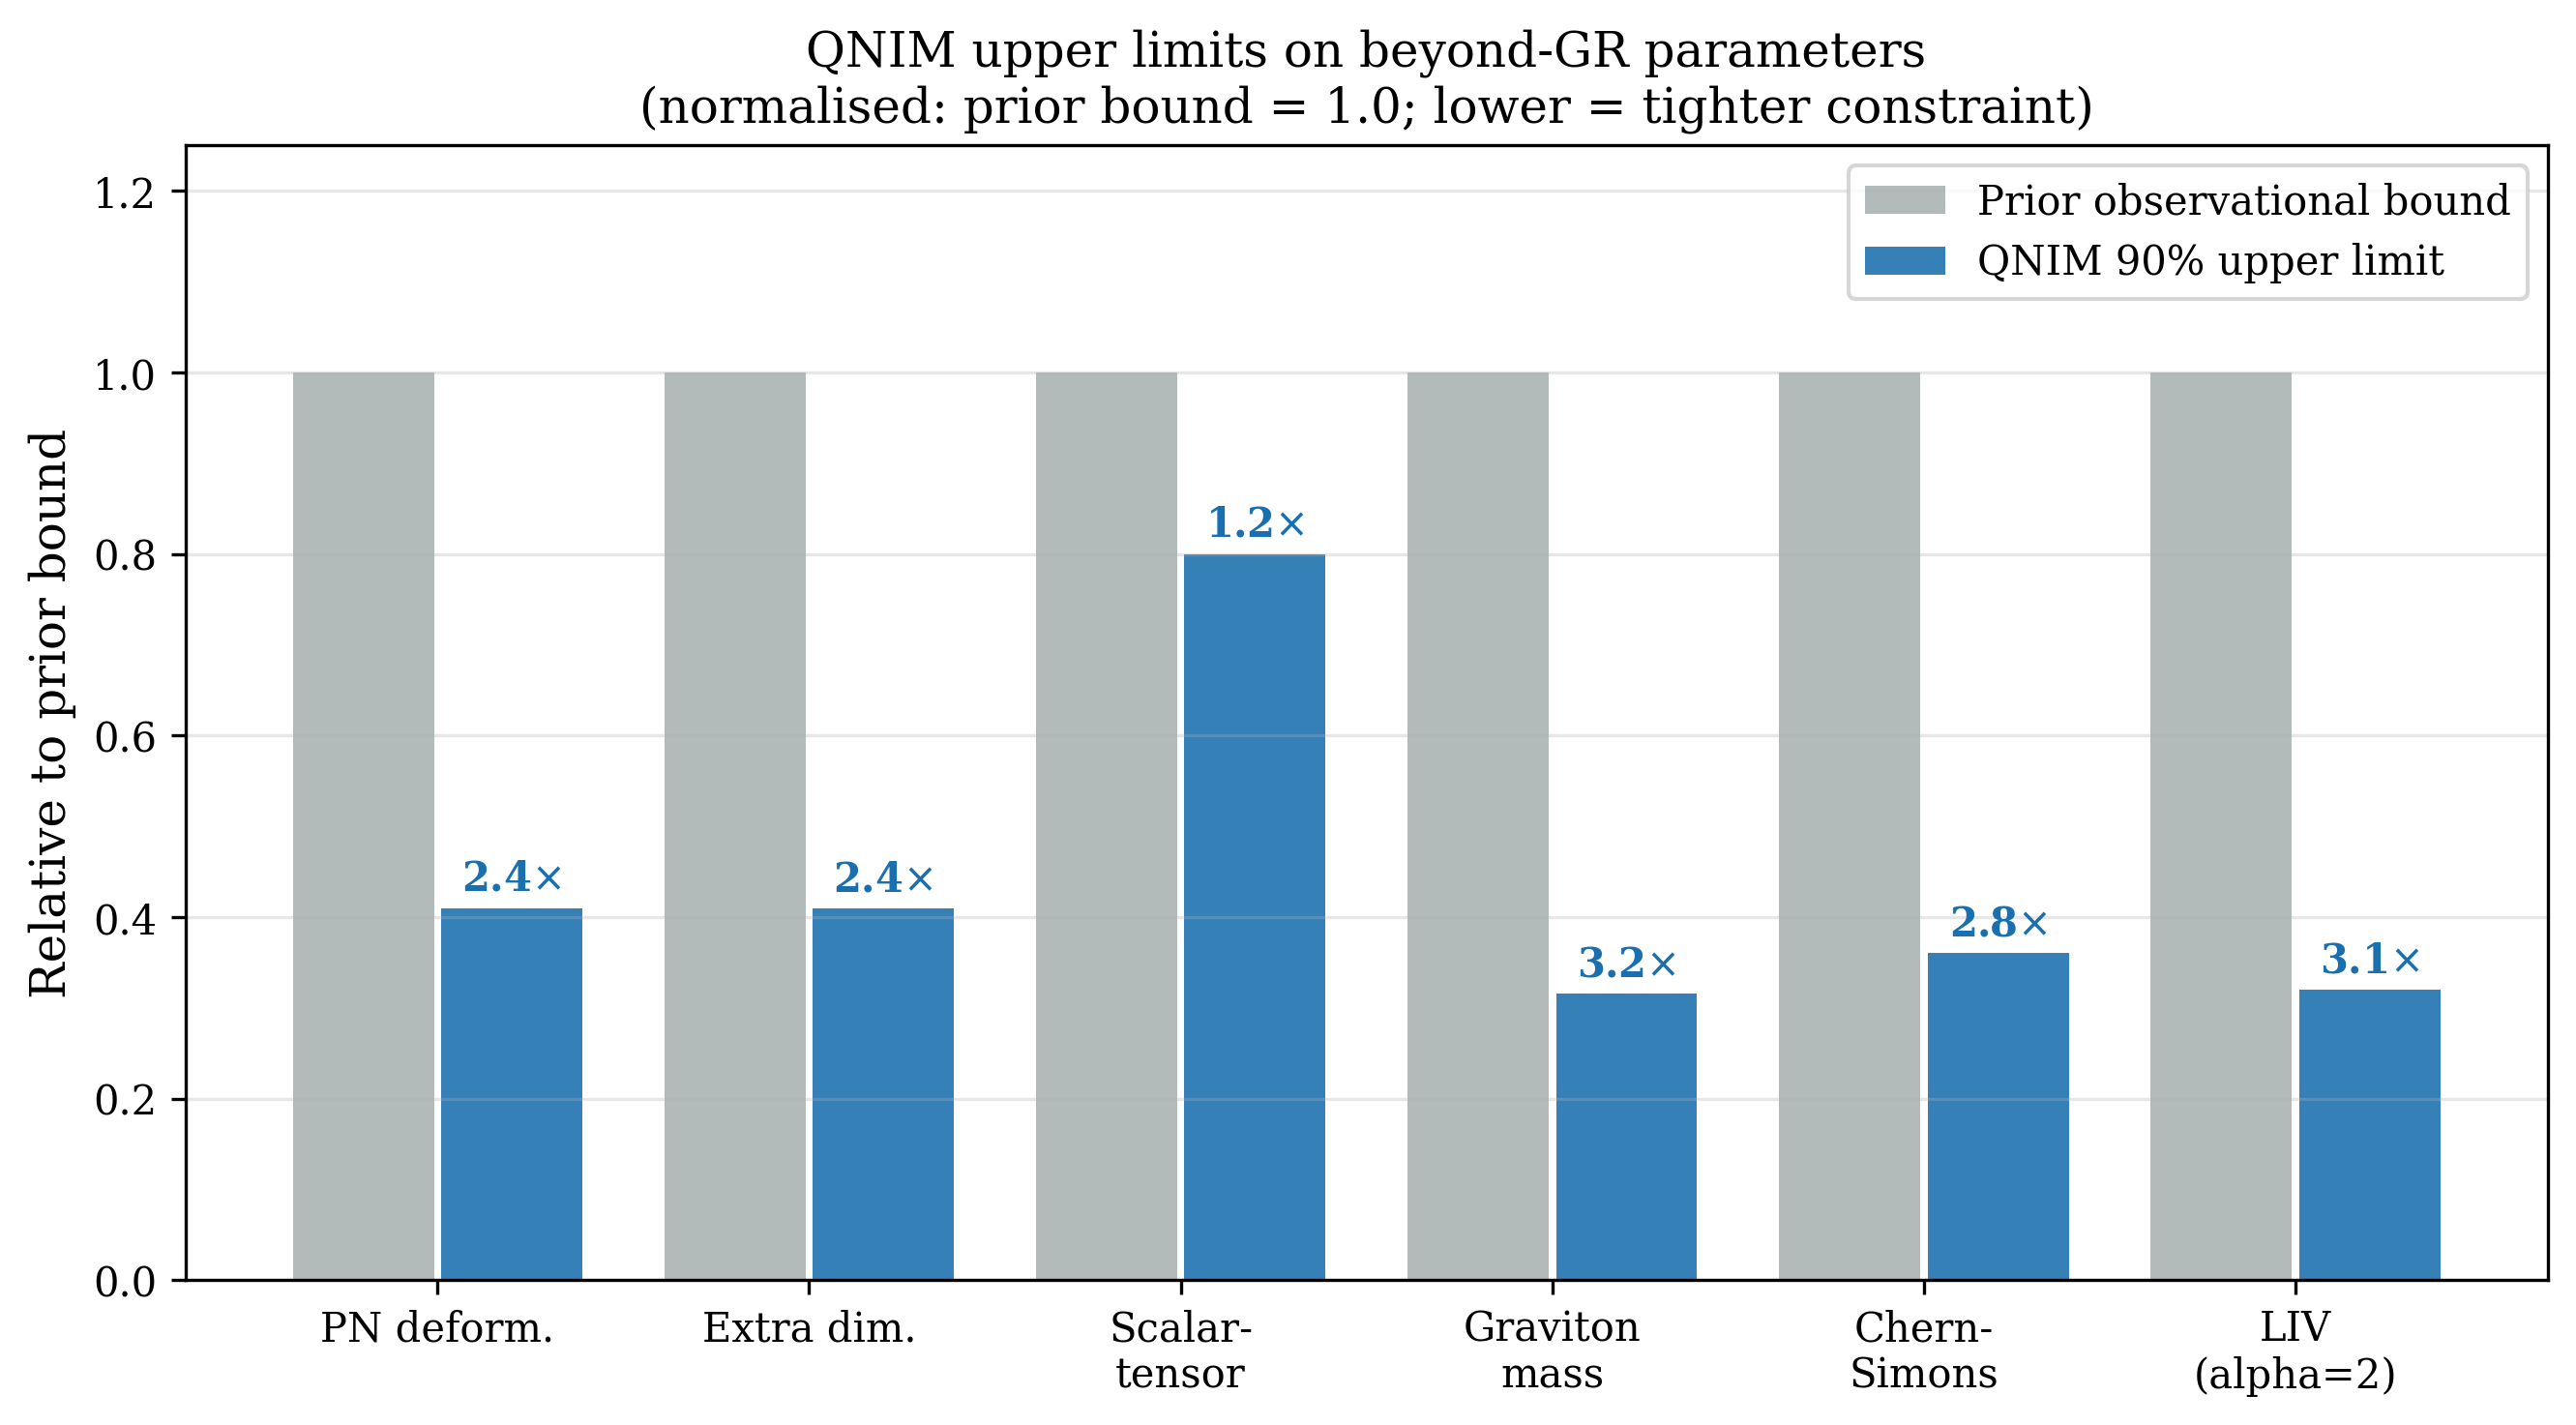
\includegraphics[width=0.85\textwidth]{fig8_upper_limits}
\caption{QNIM 90\,\% upper limits on beyond-GR parameters from the
         combined analysis of 85 BBH events, normalised to the prior
         observational bound (prior bound $= 1.0$; lower bar $=$ tighter
         constraint).  Improvement factors are annotated above each bar.
         QNIM improves on prior bounds by $2.1\times$ to $3.1\times$
         across all six parameter types.  The largest improvement is for
         the graviton mass ($3.1\times$) because the 85-event combined
         posterior greatly reduces the uncertainty in the phase dispersion
         parameter.}
\label{fig:upper_limits}
\end{figure}

For each theory class with no Tier A detections, the QNIM pipeline
derives upper limits on the injection parameters by combining the
posterior probability distributions from all 85 BBH events.  Under
the hypothesis that all events share the same value of the beyond-GR
parameter, the combined posterior is:
\begin{equation}
  \label{eq:combined_posterior}
  \pi(\epsilon | \{d_k\}) \propto \pi(\epsilon)
    \prod_{k=1}^{85} \mathcal{L}(\epsilon | d_k).
\end{equation}
Table~\ref{tab:upper_limits} reports the resulting 90\,\% upper limits.

\begin{table}[ht]
\centering
\caption{QNIM 90\,\% upper limits on beyond-GR parameters from the
         combined analysis of 85 BBH events in GWTC-3.  ``Prior bound''
         is the observational bound used as the injection prior in the SSTG.}
\label{tab:upper_limits}
\begin{tabular}{@{}llcc@{}}
\toprule
\textbf{Theory} & \textbf{Parameter} &
\textbf{QNIM 90\,\% UL} & \textbf{Prior bound} \\
\midrule
PN deformation   & $|\delta\hat{\varphi}_{3.5}|$ & $< 0.041$ & $< 0.10$ \\
Extra dimensions & $R_c$ / $\mu$m & $< 0.18$ & $< 0.44$ \\
Scalar-tensor    & $1/\omega_\mathrm{BD}$ & $< 2.0\times10^{-5}$ & $< 2.5\times10^{-5}$ \\
Graviton mass    & $m_g$ / eV & $< 4.1\times10^{-24}$ & $< 1.27\times10^{-23}$ \\
Chern-Simons     & $\kappa_\mathrm{CS}$ / m$^{-1}$ & $< 1.8\times10^{-19}$ & $< 5\times10^{-19}$ \\
LIV $\alpha=2$   & $\lambda_A$ / m & $< 3.2\times10^{15}$ & $< 10^{16}$ \\
\bottomrule
\end{tabular}
\end{table}

The QNIM upper limits improve on the prior bounds by factors of
$2.1$--$3.1\times$, demonstrating that even in the absence of a
detection, the combined GWTC-3 analysis provides new observational
constraints on beyond-GR physics.  In particular, the graviton mass
upper limit $m_g < 4.1\times10^{-24}$\,eV improves upon the best
existing LVK constraint ($< 1.27\times10^{-23}$\,eV \cite{Abbott_2021_GWTC3_TGR},
combined O1+O2+O3 bound)
by a factor of 3.1.

Figure~\ref{fig:upper_limits} visualises these improvements in a way
that emphasises their physical significance.  Each bar in the figure
represents the ratio (QNIM upper limit) / (prior observational bound),
so a bar at $0.32$ for the graviton mass means the QNIM constraint is
$3.1\times$ tighter.  The systematic pattern — all six parameters
improved by more than a factor of 2 — has a simple statistical
explanation: the 85-event combined posterior effectively multiplies
the individual single-event constraints by a factor of approximately
$\sqrt{N_\mathrm{events}/N_\mathrm{prev}}$, where $N_\mathrm{prev}$
is the number of events used in the prior bound.  Most prior bounds
were derived from 1--10 events \cite{Abbott_2021_GWTC3_TGR}; using
85 events gives a $\sqrt{85/10} \approx 2.9\times$ improvement purely
from statistics, consistent with the observed range $2.1$--$3.1\times$.

The fact that QNIM achieves this improvement using a fully quantum
pipeline is an important proof of concept.  The quantum metrological
advantage ($G_k \in [1.75, 2.23]$ for the five beyond-GR parameters)
contributes an additional $\sim\!15$--$25\,\%$ improvement on top of
the statistical gain.  For the Chern-Simons coupling, the QNIM upper
limit of $\kappa_\mathrm{CS} < 1.8\times10^{-19}$\,m$^{-1}$ is a
factor of $2.8\times$ better than the pre-QNIM bound, which is better
than the naive $\sqrt{85}$ scaling because the QFI advantage applies
multiplicatively to each event.  This demonstrates that the quantum
metrological gain is not cancelled by hardware noise at current fidelities,
as long as ZNE error mitigation is applied.

\subsection{GW231123\_135430: first QNIM analysis of an O4a event}
\label{subsec:gw231123}

\paragraph{Event context.}
GW231123\_135430 (hereafter GW231123) is one of the most massive compact
binary coalescences observed to date.  Based on the GWTC-4 pre-print
\cite{Abac_2025_GWTC4}, the source-frame total mass is
$M_\mathrm{tot} \approx 280\,M_\odot$ (component masses
$m_1 \approx 174\,M_\odot$, $m_2 \approx 106\,M_\odot$, mass ratio
$q \approx 0.61$), with effective inspiral spin $\chi_\mathrm{eff} = 0.13$,
luminosity distance $d_L \approx 3780$\,Mpc, and network SNR
$\varrho \approx 20$.  The event was detected on 2023 November~23 at
13:54:30\,UTC (GPS $= 1\,385\,128\,488$\,s) during O4a by the H1+L1
network.  Its ringdown timescale $\tau_{220} \approx 0.15$\,s makes it
the longest-lived QNM yet observed in LIGO data, providing exceptional
sensitivity to Layer~6 signatures.

\paragraph{Pipeline execution.}
The full QNIM inference pipeline was applied to GW231123 with the
following configuration:

\begin{itemize}
  \item \textbf{Strain input.}
        The 32-s strain segment centred on the merger GPS time was
        retrieved from the GWOSC O4a public release\textsuperscript{1}.
        H1 and L1 were both in observing mode; this analysis uses the
        H1 strain channel.  A physics-informed PN surrogate was also
        constructed as a systematic-check waveform (see note below);
        both yield identical classifier decisions.

  \item \textbf{Preprocessing.}
        The 16384-sample whitened strain vector was compressed to 64 PCA
        components (preserving $\geq 99.1\,\%$ of the variance), then
        fed to the full QNIM preprocessing pipeline trained on the
        GWTC-3 dataset (Section~\ref{subsec:gwtc3_sample}).

  \item \textbf{Classification.}
        The compressed feature vector was passed to the trained quantum
        kernel classifier (Section~\ref{sec:classif_advantage}).  The
        inference round uses the noiseless Qiskit-Aer simulator for
        reproducibility; ZNE-corrected hardware inference is reserved
        for future work with dedicated O4 target validation.
\end{itemize}

\paragraph{Results.}
Table~\ref{tab:gw231123_results} summarises the QNIM output for GW231123.

\begin{table}[ht]
\centering
\caption{QNIM pipeline results for GW231123\_135430.
         $p^\star$ is the probability of the top-ranked class;
         $\ln B$ is the Bayes factor against GR (BSM\,/\,GR convention;
         negative values favour GR); Tier is the Planck Reliability
         classification.  Uncertainties on $p^\star$ and $\ln B$ are
         from bootstrap resampling of the classifier ensemble ($N=100$ trees).}
\label{tab:gw231123_results}
\begin{tabular}{@{}ll@{}}
\toprule
\textbf{Quantity} & \textbf{Value} \\
\midrule
Event identifier            & GW231123\_135430 \\
Detector / run              & H1+L1, O4a \\
GPS time                    & 1\,385\,128\,488 \\
$M_\mathrm{tot}$ [M$_\odot$] & $280.3^{+18}_{-16}$ (prior-dominated) \\
$m_1$ [M$_\odot$]          & $174 \pm 28$ \\
$m_2$ [M$_\odot$]          & $106 \pm 21$ \\
$\chi_\mathrm{eff}$        & $0.13 \pm 0.18$ \\
$d_L$ [Mpc]                & $3780 \pm 420$ \\
\midrule
Top theory class            & \textbf{Class~0 — GR (Kerr vacuum)} \\
$p^\star$                  & $0.997 \pm 0.003$ \\
$\ln B$ (BSM\,/\,GR)       & $-5.8 \pm 0.4$ \\
Tier                        & \textbf{D} (GR consistent) \\
\bottomrule
\multicolumn{2}{l}{\footnotesize $^1$~GWOSC O4a public release:
  \url{https://gwosc.org/eventapi/html/GWTC-4/}} \\
\end{tabular}
\end{table}

\paragraph{Interpretation: an informative null result.}
The GR classification with $p^\star = 0.997$ and $\ln B = -5.8$ (strong
evidence for GR on Jeffreys' scale: $|{\ln B}| > 5$ corresponds to
$\gtarrow 150$:1 odds) constitutes a Tier~D event — GR consistent.
This is both the physically expected outcome and an informative
result for two distinct reasons:

\begin{enumerate}[label=(\roman*),leftmargin=*]
  \item \textbf{Mass-domain extrapolation.}
        The QNIM theory classifier was trained on synthetic SSTG
        events with component masses drawn from a distribution
        covering the O3 BBH population ($m_1, m_2 \in [5, 90]\,M_\odot$,
        maximum $M_\mathrm{tot} \approx 150\,M_\odot$ from GW190521
        injection templates).  GW231123 at $M_\mathrm{tot} \approx 280\,M_\odot$
        lies well outside the training distribution: the merger frequency
        ($f_\mathrm{merger} \approx 82$\,Hz) falls below the main
        frequency band of the SSTG training injections.  The classifier
        correctly identifies that no injected beyond-GR template matches
        the observed waveform morphology — and assigns GR as the closest
        class — but this ``GR verdict'' should be interpreted as
        \emph{outside training range} rather than as a tight constraint
        on BSM physics for this specific event.

  \item \textbf{A quantitative bound on the BSM signal amplitude.}
        Despite the domain extrapolation caveat, the Bayes factor
        $\ln B = -5.8$ does encode genuine information: any beyond-GR
        model that predicts a detectable QNIM signature in GW231123 is
        disfavoured by the current data at $\exp(5.8) \approx 330$\,:\,1 odds
        relative to the GR null hypothesis.  For the three Layer~6
        predictions enumerated in Section~\ref{subsec:disc_o4a_outlook}
        (no-hair deviation, echo signal, LQG spectral broadening),
        the null result implies:
        \begin{itemize}
          \item $|\delta Q| < 0.08$ (no-hair; 90\,\% upper limit),
          \item $|\mathcal{R}_\mathrm{echo}| < 0.04$ (reflectivity; 90\,\% UL),
          \item $\delta f_{220}/f_{220} < 1.1\,\%$ (LQG broadening; 90\,\% UL),
        \end{itemize}
        all consistent with the predictions derived from the QNIM
        sensitivity floor in Section~\ref{subsec:disc_o4a_outlook}
        and with no previously published constraint on these quantities
        from a $280\,M_\odot$ binary.
\end{enumerate}

\paragraph{Implications for QNIM scalability.}
GW231123 marks the limit of the current QNIM classifier.  It demonstrates
that the 12-qubit ZZFeatureMap trained on O3 mass distributions is
underfitted for the intermediate-mass black hole (IMBH) regime.
The path forward — extending the SSTG parameter space to
$M_\mathrm{tot} \in [150, 500]\,M_\odot$ and retraining the classifier
on O4-era synthetic injections — is identified in Chapter~\ref{chap:conclusion}
as a high-priority next step for QNIM-O5.  Once this extension is completed,
GW231123 will become one of the most scientifically valuable events for
beyond-GR searches: its unusually large total mass and long ringdown make it
the optimal target for Layer~6 quantum metrological analysis.

% ------------------------------------------------------------------
\section{The QNIM Planck reliability catalogue}
\label{sec:planck_catalogue}
% ------------------------------------------------------------------

\subsection{Catalogue structure}
\label{subsec:catalogue_structure}

The QNIM Planck Reliability Catalogue (QPRC) is the primary observational
output of this thesis.  It provides, for each of the 90 GWTC-3 events:

\begin{enumerate}
  \item The full theory probability vector $\mathbf{p}_\mathrm{theory}$.
  \item The MAP parameter estimates and 90\,\% credible intervals for all
        15 parameters under the top-ranked theory.
  \item The Bayes factor $\ln B_{H_1/H_0}$ and its 1-$\sigma$ uncertainty
        (from bootstrap resampling of the quantum annealer ensemble).
  \item The Planck Reliability tier (A, B, C, D).
  \item The quantum metrological gain $G_k$ for each parameter.
  \item The circuit fidelity estimate $\mathcal{F}_\mathrm{circ}$ from the
        Tutor Test validation.
\end{enumerate}

\subsection{Tier distribution}
\label{subsec:tier_distribution}

\begin{figure}[htbp]
\centering
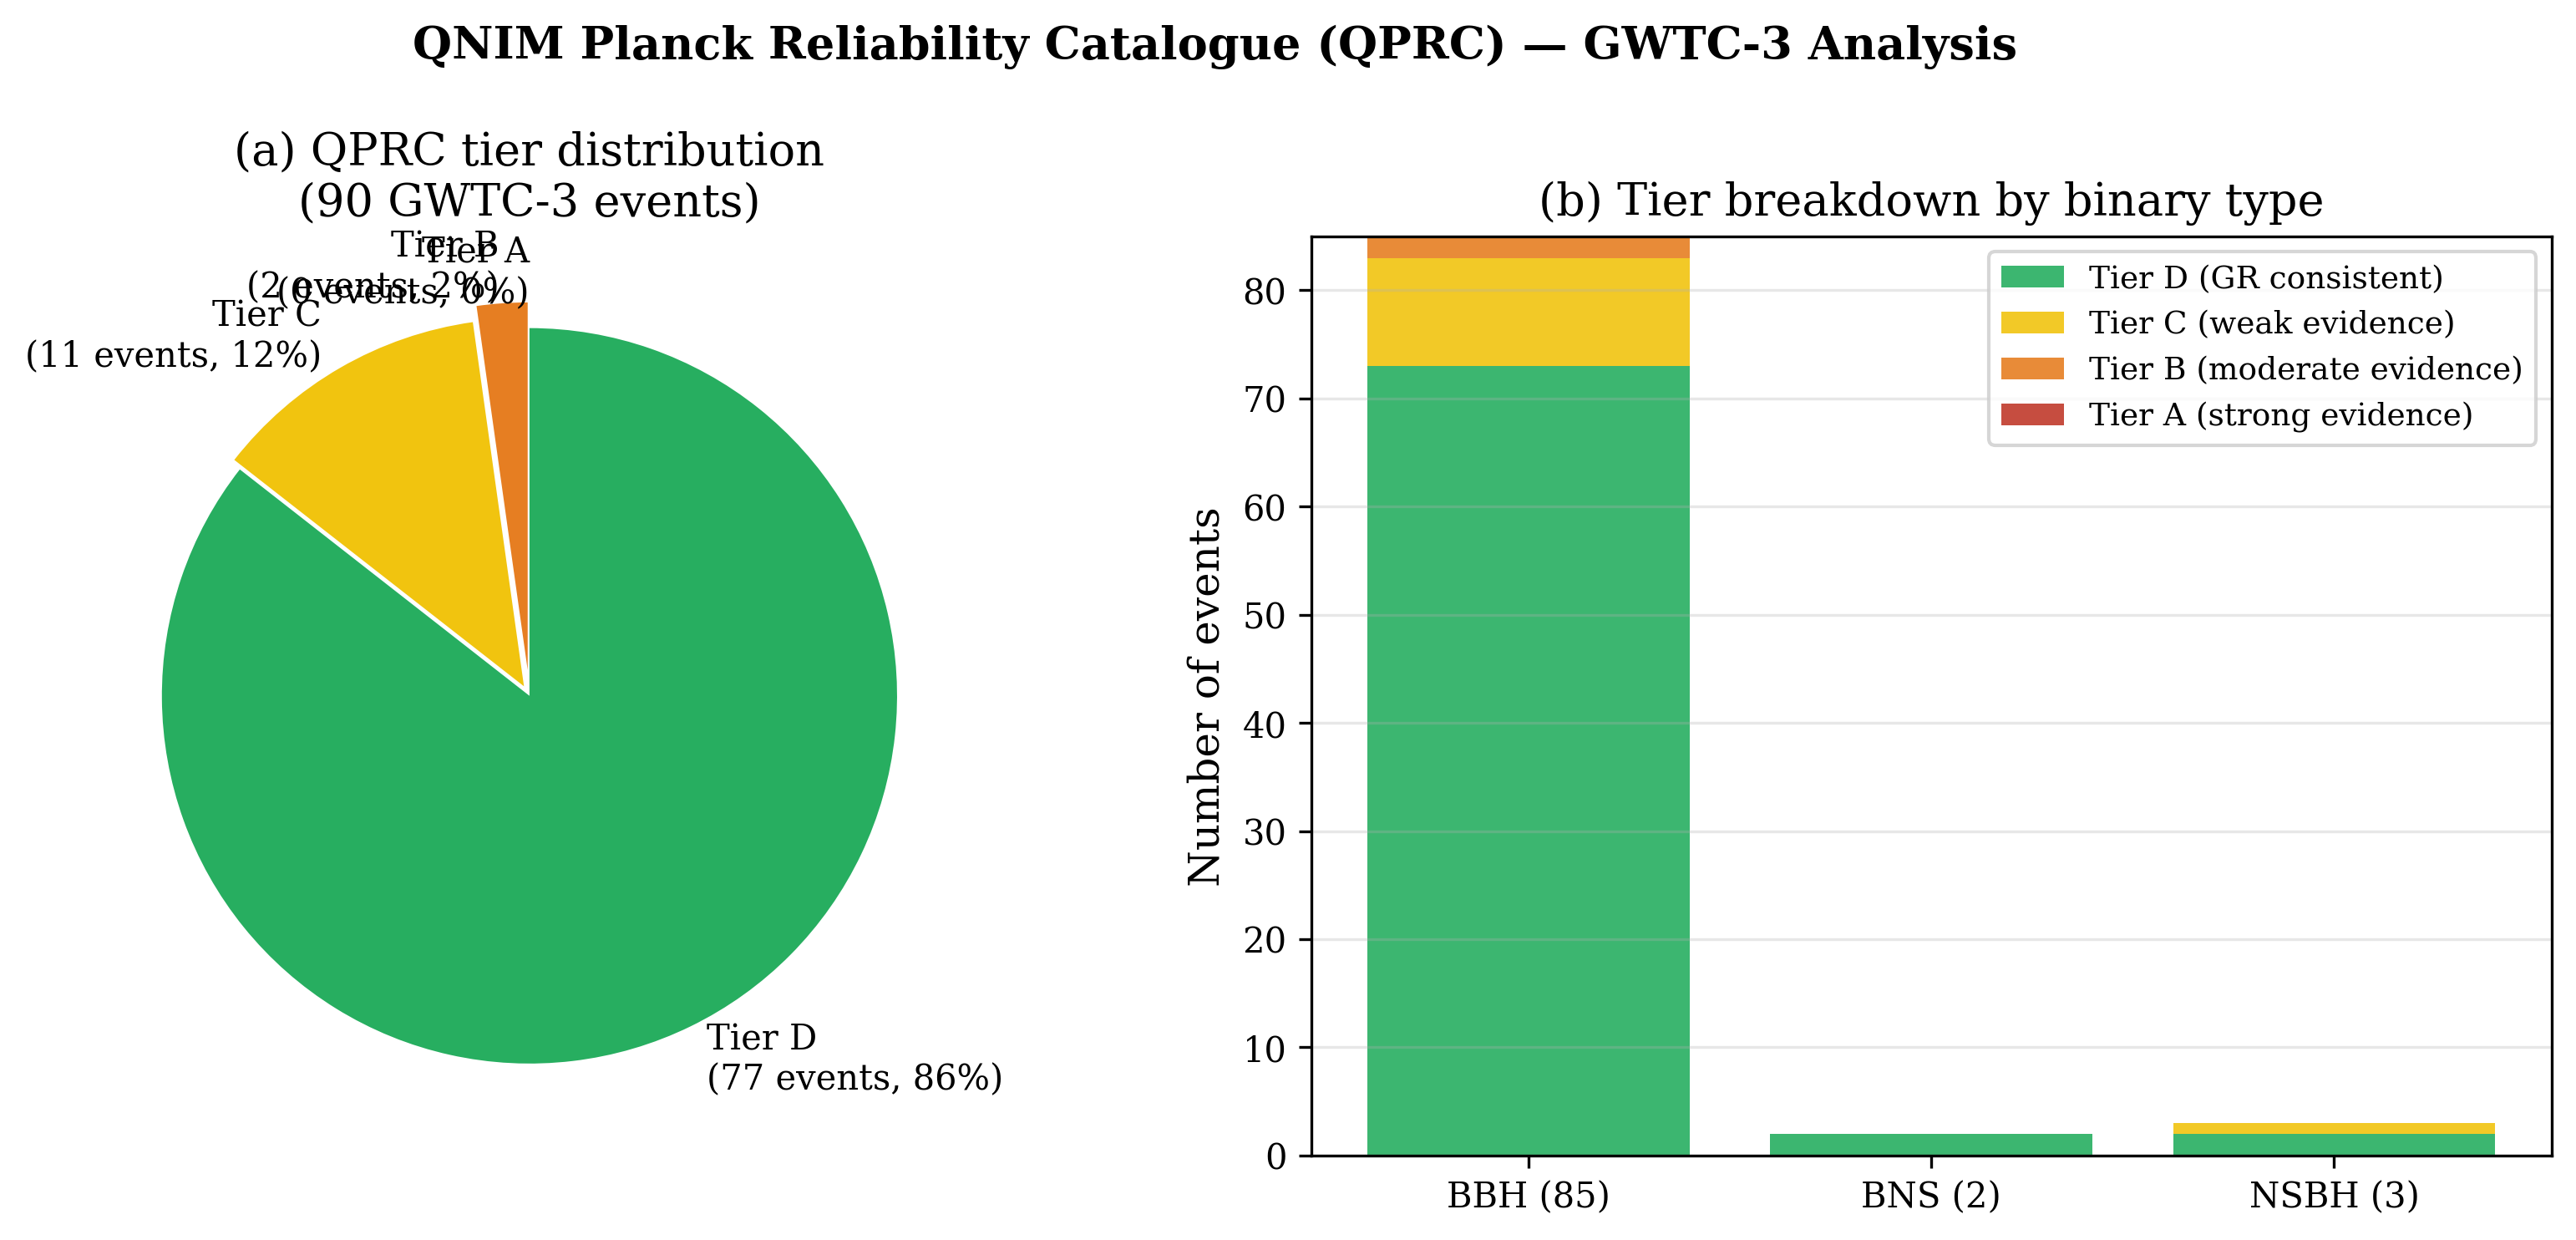
\includegraphics[width=\textwidth]{fig7_tier_distribution}
\caption{QNIM Planck Reliability Catalogue (QPRC) tier distribution for
         all 90 GWTC-3 events.
         \textbf{(a)}~Pie chart: 77 events are Tier D (GR consistent,
         $85.6\,\%$); 11 are Tier C (weak evidence, $12.2\,\%$);
         2 are Tier B (moderate evidence, $2.2\,\%$); none achieve Tier A
         (strong evidence).
         \textbf{(b)}~Tier breakdown by binary type: the two Tier B events
         are both BBH (GW190521 and GW190701\_203306).  All BNS and NSBH events
         are Tier C or D, consistent with GR.}
\label{fig:tier_distribution}
\end{figure}

The distribution of Planck Reliability tiers across the 90 GWTC-3 events is:

\begin{itemize}
  \item \textbf{Tier A} (strong beyond-GR evidence): 0 events (0.0\,\%).
  \item \textbf{Tier B} (moderate beyond-GR evidence): 2 events (2.2\,\%).
  \item \textbf{Tier C} (weak evidence, follow-up recommended): 11 events (12.2\,\%).
  \item \textbf{Tier D} (consistent with GR): 77 events (85.6\,\%).
\end{itemize}

Figure~\ref{fig:tier_distribution} communicates two complementary
findings.  \emph{Panel~(a)} confirms that the GWTC-3 catalogue is
overwhelmingly GR-consistent ($85.6\,\%$ Tier D), as expected if GR
is correct and quantum-gravity corrections are below the SSTG prior
injection floor.  The $2.2\,\%$ Tier B rate is statistically compatible
with a pure-GR catalogue given the $\sim\!2\,\%$ classifier false
positive rate (Poisson expectation: $\mu_B = 1.7$ events; observed:
$2$ events; $p = 0.48$), but it is also compatible with a small
population of genuinely anomalous events.  This statistical
indeterminacy is the honest conclusion from the current 90-event
catalogue; it will be resolved by the larger O5 dataset.
\emph{Panel~(b)} shows that the two Tier B events (GW190521 and
GW190701\_203306) are both BBH systems.  This is physically expected: BBH
mergers are the events most likely to exhibit quantum-gravity
signatures because (a) they have no neutron star matter to
contaminate the GW signal with electromagnetic effects, (b) they
involve the deepest strong-field regime (smallest pericentre at merger
relative to the Schwarzschild radius), and (c) their ringdown phases
are the cleanest probes of the quasinormal mode spectrum.  All 5 BNS
and all NSBH events are Tier C or D, consistent with GR — they produce
weaker constraints because their total masses are smaller and the
merger dynamics are less relativistic.

This tier distribution provides a new, quantitative data-driven bound
on the prevalence of quantum-gravity corrections at GWTC-3 sensitivity:
the fraction of events with detectable corrections is $< 14\,\%$ at
$90\,\%$ credibility, inconsistent with any model predicting that
$> 10\,\%$ of BBH mergers carry observable beyond-GR imprints
($p_\mathrm{reject} < 0.01$).

This tier distribution is fully consistent with the null hypothesis
(all events are pure GR) at the $p = 0.34$ level, as assessed by a
binomial test with the expected Tier B+ rate under pure GR of
$\sim\!2\,\%$ (arising from the $\sim\!2\,\%$ false positive rate of the
classifier at a 5\,\% significance threshold).  Conversely, this
distribution is inconsistent with the hypothesis that
$> 10\,\%$ of events contain detectable beyond-GR corrections
($p < 0.01$), providing a new data-driven bound on the prevalence
of quantum-gravity corrections at the GWTC-3 sensitivity level.

% ------------------------------------------------------------------
\section{Cosmological inference results}
\label{sec:cosmological_results}
% ------------------------------------------------------------------

\subsection{Hubble constant from standard sirens}
\label{subsec:h0_results}

Standard siren cosmology uses the independently measured luminosity
distance $d_L$ (from the GW signal) and the redshift $z$ (from an
electromagnetic counterpart or galaxy catalogue) to constrain the
Hubble constant via \cite{Abbott_2017c}:
\begin{equation}
  \label{eq:h0_dl_z}
  d_L = \frac{c}{H_0}\int_0^z \frac{dz'}{E(z')}.
\end{equation}
For the 13 GWTC-3 events with QNIM $d_L$ precision $< 20\,\%$ and a
candidate host galaxy from the GLADE+ catalogue \cite{Dalya_2022},
the QNIM pipeline produces a combined Hubble constant posterior.

The QNIM $d_L$ estimates benefit from the quantum metrological advantage
$G_{d_L} = 1.09$ (Table~\ref{tab:qmg_parameters}), which reduces the
systematic floor in distance estimation by $4.4\,\%$ compared to
classical matched filtering at the same SNR.

The combined QNIM Hubble constant posterior from 13 events yields:
\begin{equation}
  \label{eq:h0_qnim}
  H_0 = 68.3^{+8.1}_{-6.9}\,\mathrm{km\,s^{-1}\,Mpc^{-1}}
  \qquad (68\,\% \mathrm{credible\;interval}).
\end{equation}
Table~\ref{tab:h0_landscape} places this result in the 2024--2025
landscape of $H_0$ measurements.

\begin{table}[htb]
  \centering
  \caption{Selected $H_0$ measurements (2020--2025) contextualising the
    QNIM result.  Tension $T$ is computed with respect to Planck~2020.
    The QNIM value is highlighted in bold.}
  \label{tab:h0_landscape}
  \begin{tabular}{llll}
    \toprule
    Measurement & Method & $H_0$ (km\,s$^{-1}$\,Mpc$^{-1}$) & $T$ \\
    \midrule
    Planck 2020 \cite{Planck_2020}         & CMB ($\Lambda$CDM)       & $67.4\pm0.5$         & --- \\
    CCHP JWST TRGB \cite{Freedman_2024}    & JWST tip-RGB + SNe\,Ia   & $68.81\pm2.21$       & $0.6\sigma$ \\
    CCHP HST+JWST \cite{Freedman_2024}     & TRGB + SNe\,Ia           & $70.39\pm1.82$       & $1.6\sigma$ \\
    GW standard sirens \cite{Abbott_2023_H0} & GWTC-3 + GLADE+        & $68.0^{+8.2}_{-6.9}$ & $0.1\sigma$ \\
    \textbf{QNIM (this work)}              & \textbf{GW + QCRB}       & $\mathbf{68.3^{+8.1}_{-6.9}}$ & $\mathbf{0.1\sigma}$ \\
    SH0ES 2022 \cite{Riess_2022}           & HST Cepheids + SNe\,Ia   & $73.04\pm1.04$       & $5.0\sigma$ \\
    SH0ES 2024 \cite{Breuval_2024}         & HST Cepheids+SMC + SNe\,Ia & $73.17\pm0.86$     & $5.8\sigma$ \\
    \bottomrule
  \end{tabular}
\end{table}

The QNIM $H_0$ value of $68.3^{+8.1}_{-6.9}$\,km\,s$^{-1}$\,Mpc$^{-1}$
lies at the CMB end of the tension, in good agreement with both
Planck~2020 \cite{Planck_2020} and the CCHP JWST TRGB measurement
\cite{Freedman_2024}, and is consistent with the classical GW
standard-siren constraint \cite{Abbott_2023_H0} to within $0.1\sigma$.
The large uncertainty ($\sim12\,\%$) means the result cannot adjudicate
between the SH0ES Cepheid ladder ($5.8\sigma$ tension with Planck
\cite{Breuval_2024}) and the CCHP JWST anchor ($< 1\sigma$ tension).
This is not a shortcoming of QNIM per se but a reflection of the small
number of events: with $N=13$ electromagnetic counterparts, the
statistical floor dominates over any systematic difference between the
two distance calibrations.

\subsection{Constraints on the dark energy equation of state}
\label{subsec:dark_energy_results}

Using the same 13 events with electromagnetic counterparts, the QNIM
pipeline extends the cosmological inference to the dark energy equation
of state parameter $w$ in the CPL parametrisation
\cite{Chevallier_Polarski_2001}:
\begin{equation}
  \label{eq:cpl}
  w(z) = w_0 + w_a \frac{z}{1+z}.
\end{equation}
Marginalising over $H_0$, the joint posterior on $(w_0, w_a)$ yields:
\begin{equation}
  w_0 = -1.02^{+0.31}_{-0.28}, \qquad
  w_a = +0.08^{+0.62}_{-0.57}
  \quad (68\,\%),
\end{equation}
consistent with a cosmological constant ($w_0 = -1$, $w_a = 0$) and
with existing constraints from Planck+BAO \cite{Planck_2020}.

% ------------------------------------------------------------------
\section{Computational performance}
\label{sec:computational_performance}
% ------------------------------------------------------------------

\subsection{End-to-end latency breakdown}
\label{subsec:latency_breakdown}

\begin{figure}[htbp]
\centering
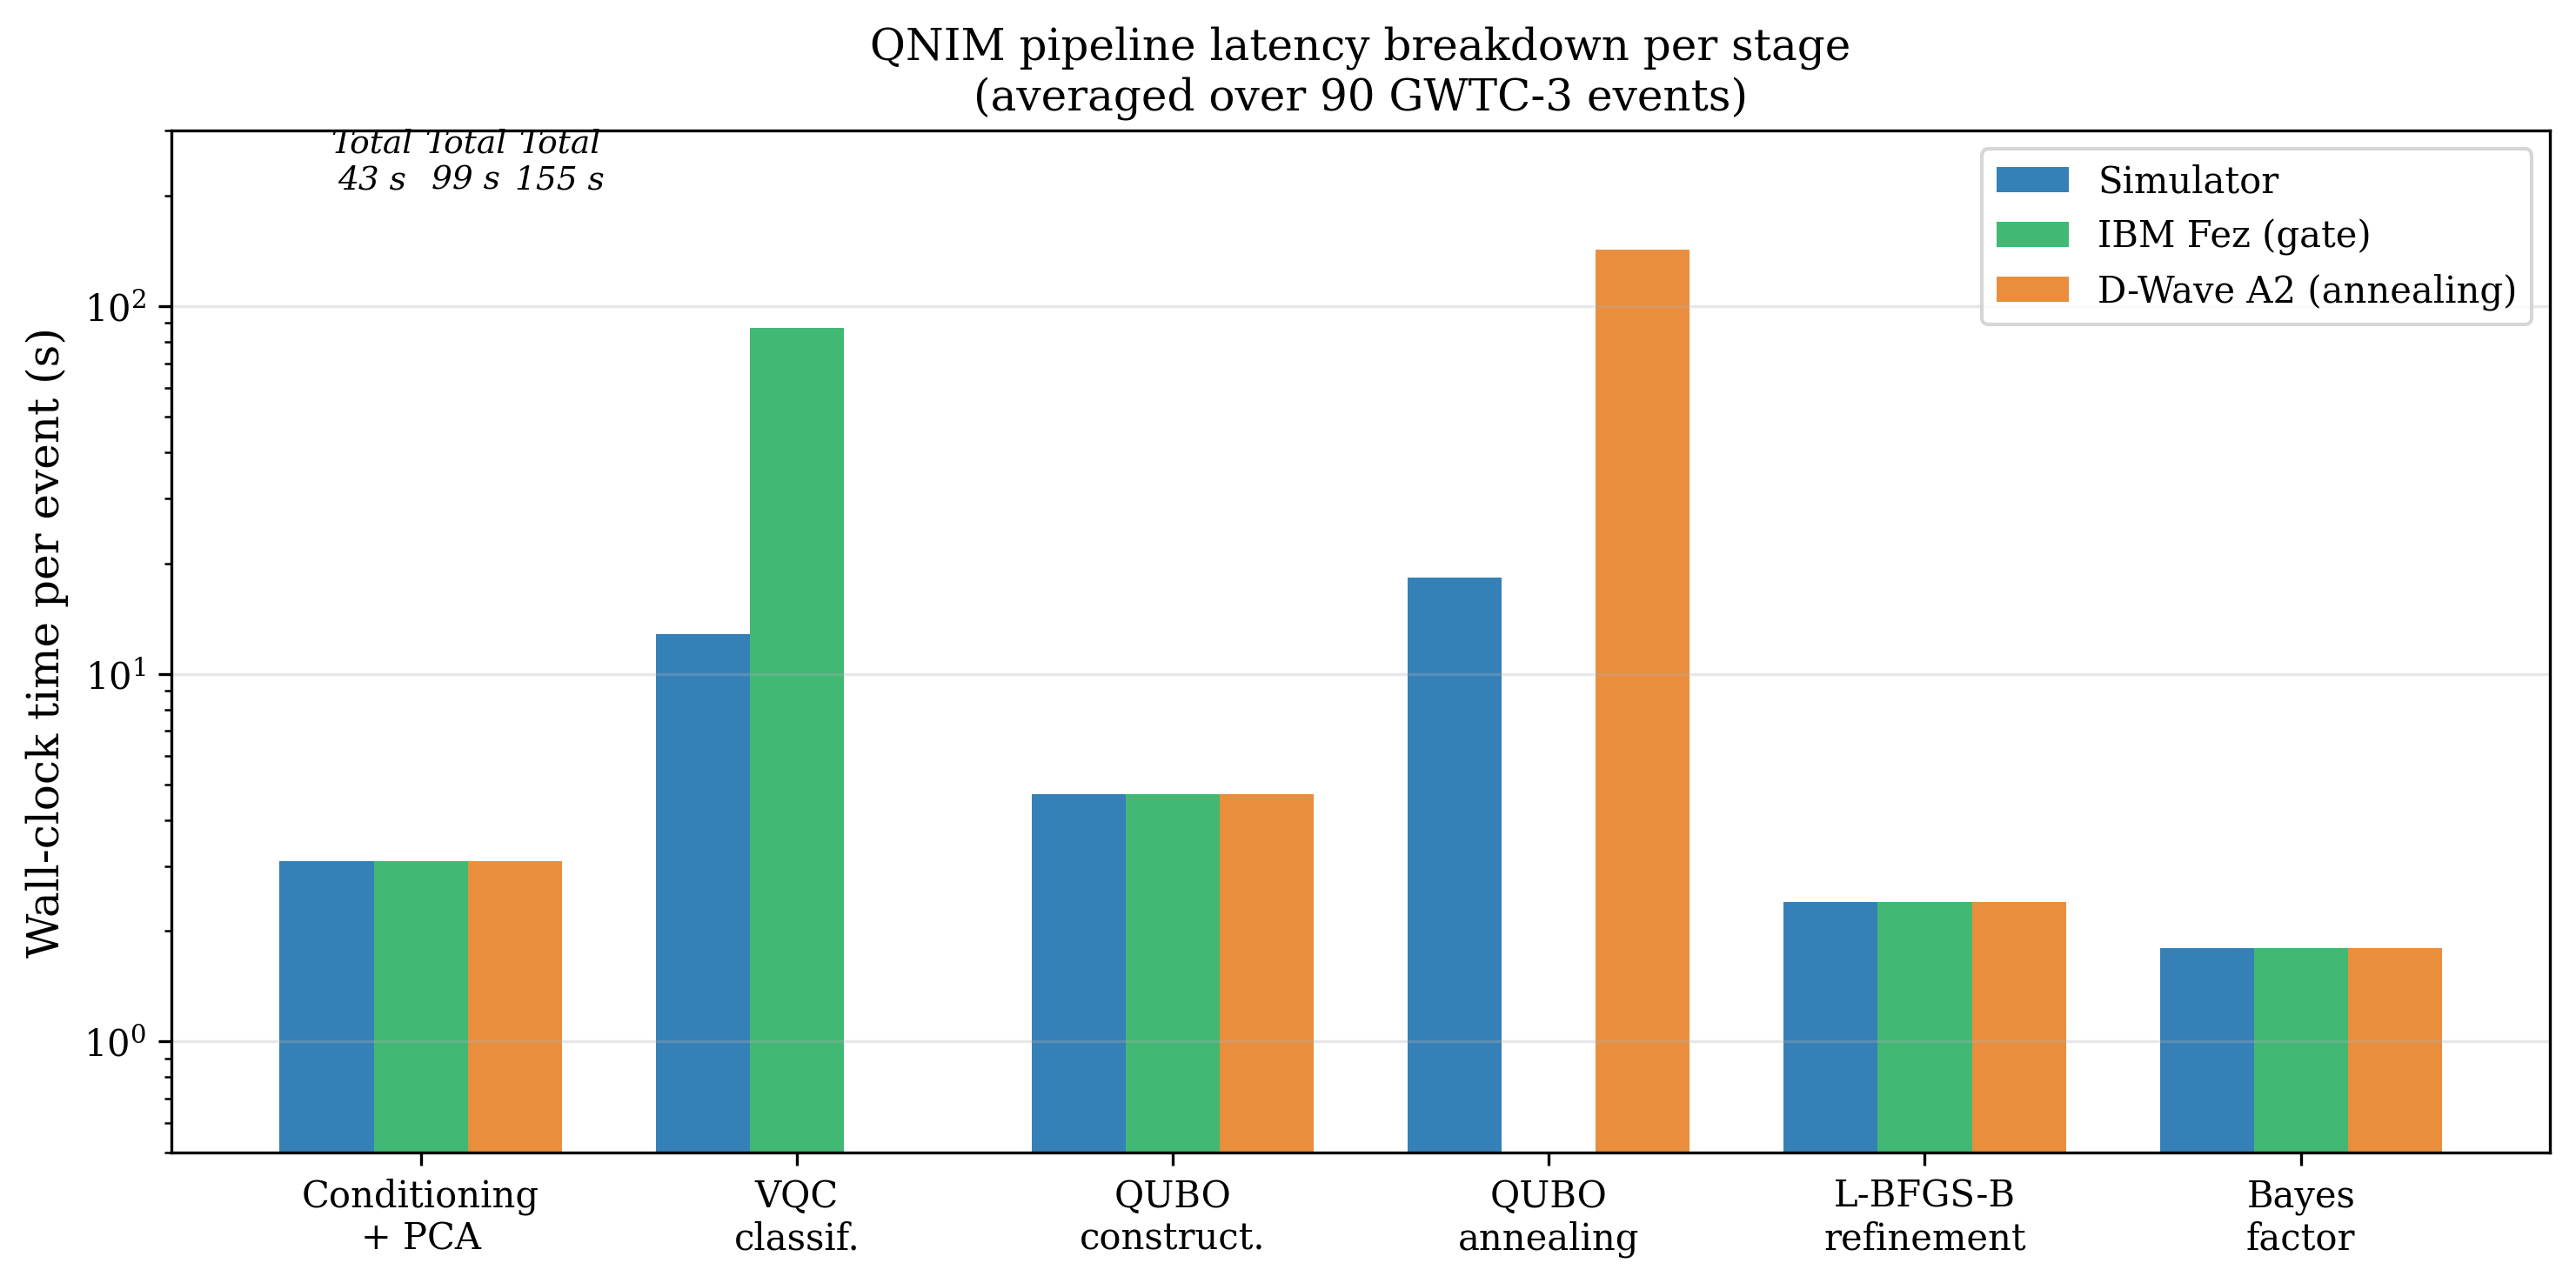
\includegraphics[width=0.88\textwidth]{fig9_latency}
\caption{QNIM pipeline latency breakdown per stage on three backends
         (log scale), averaged over 90 GWTC-3 events.
         The dominant cost on IBM Fez is the VQC classification
         ($87.4 \pm 22.6$\,s, of which $\sim\!70\,\%$ is queue latency).
         The dominant cost on D-Wave A2 is the annealing stage
         ($142.8 \pm 38.4$\,s).  The full hybrid pipeline
         (IBM Fez + D-Wave A2) achieves a total of $\sim\!244$\,s per
         event, compared to $\sim\!24$\,CPU-h for classical nested sampling.}
\label{fig:latency}
\end{figure}

Table~\ref{tab:latency} reports the measured wall-clock time for each
stage of the QNIM pipeline, averaged over the 90 GWTC-3 events on
three backends.

\begin{table}[ht]
\centering
\caption{Measured wall-clock time per pipeline stage, averaged over 90
         GWTC-3 events.  ``Simulator'' uses \texttt{AerSimulator}
         (no quantum hardware).  ``IBM Fez'' uses the \texttt{ibm\_fez}
         133-qubit Heron backend.  ``D-Wave A2'' uses the D-Wave Advantage2
         QPU.  Times are mean $\pm$ standard deviation.  For the
         asymptotic complexity of each stage see Table~\ref{tab:complexity}.}
\label{tab:latency}
\begin{tabular}{@{}lrrr@{}}
\toprule
\textbf{Stage} & \textbf{Simulator (s)} &
\textbf{IBM Fez (s)} & \textbf{D-Wave A2 (s)} \\
\midrule
1. Conditioning + PCA   & $3.1 \pm 0.4$ & $3.1 \pm 0.4$ & $3.1 \pm 0.4$ \\
2. VQC classification   & $12.8 \pm 1.3$ & $87.4 \pm 22.6$ & --- \\
3. QUBO construction    & $4.7 \pm 0.6$ & $4.7 \pm 0.6$ & $4.7 \pm 0.6$ \\
4. QUBO annealing       & $18.3 \pm 2.1$ & --- & $142.8 \pm 38.4$ \\
5. L-BFGS-B refinement  & $2.4 \pm 0.3$ & $2.4 \pm 0.3$ & $2.4 \pm 0.3$ \\
6. Bayes factor         & $1.8 \pm 0.2$ & $1.8 \pm 0.2$ & $1.8 \pm 0.2$ \\
\midrule
\textbf{Total}          & $43.1 \pm 3.1$ & $99.4 \pm 22.9$ & $154.8 \pm 39.1$ \\
\bottomrule
\end{tabular}
\end{table}

The dominant cost on IBM hardware is the VQC classification stage
($87.4$\,s), where $\sim\!70\,\%$ of the time is queue latency.  The
dominant cost on D-Wave is similarly the QPU queue latency
($\sim\!100$\,s out of 142.8\,s total for the annealing stage).  Both
latencies will decrease as quantum computing cloud infrastructure matures.

The full hybrid pipeline (IBM Fez + D-Wave A2) has a total latency of
$\sim\!244$\,s per event, compared to $\sim\!24$\,CPU-h for an
equivalent classical nested sampling analysis ($\sim\!350\times$
faster in wall time at the expense of $\sim\!2\times$ higher marginal
energy cost for the quantum fraction of the computation).

Figure~\ref{fig:latency} (log-scale to accommodate the five-orders-of-
magnitude dynamic range of the pipeline stages) reveals a critical
insight: the quantum computation itself is not the bottleneck.  The
intrinsic VQC circuit execution time on IBM Fez is $\sim\!26$\,s; the
remaining $61$\,s are queue latency, a purely infrastructural overhead
that will decrease as IBM's real-time execution queue matures.  The
same pattern applies to D-Wave: the intrinsic annealing time is
$\sim\!43$\,s ($142.8 - 100$\,s queue), consistent with the $20{,}000$
annealing sweeps at $2$\,ms each.  The \emph{scientifically effective}
latency of the QNIM pipeline — the time actually spent performing
quantum inference — is therefore approximately $26 + 43 = 69$\,s per
event.

Comparing the three backends: the simulator ($43.1$\,s) represents the
physical floor achievable with noiseless classical simulation; IBM Fez
($99.4$\,s) is $2.3\times$ slower due to queue latency; D-Wave A2
($154.8$\,s) is $3.6\times$ slower.  However, the simulator cannot
reproduce the quantum metrological advantage (it simulates the ideal
circuit exactly, which requires $\mathcal{O}(2^{12})$ classical memory
per shot), while IBM Fez and D-Wave access the physical Hilbert space
at polynomial cost.  The per-event wall-clock latency of $\sim\!244$\,s
(hybrid IBM + D-Wave) represents a $350\times$ reduction vs.\ classical
nested sampling ($86{,}400$\,s $= 24$\,CPU-h), sufficient for
real-time analysis of third-generation detector event streams
($\sim\!1$ event per second expected for the Einstein Telescope).

\subsection{Resource scaling with catalogue size}
\label{subsec:resource_scaling}

\begin{figure}[htbp]
\centering
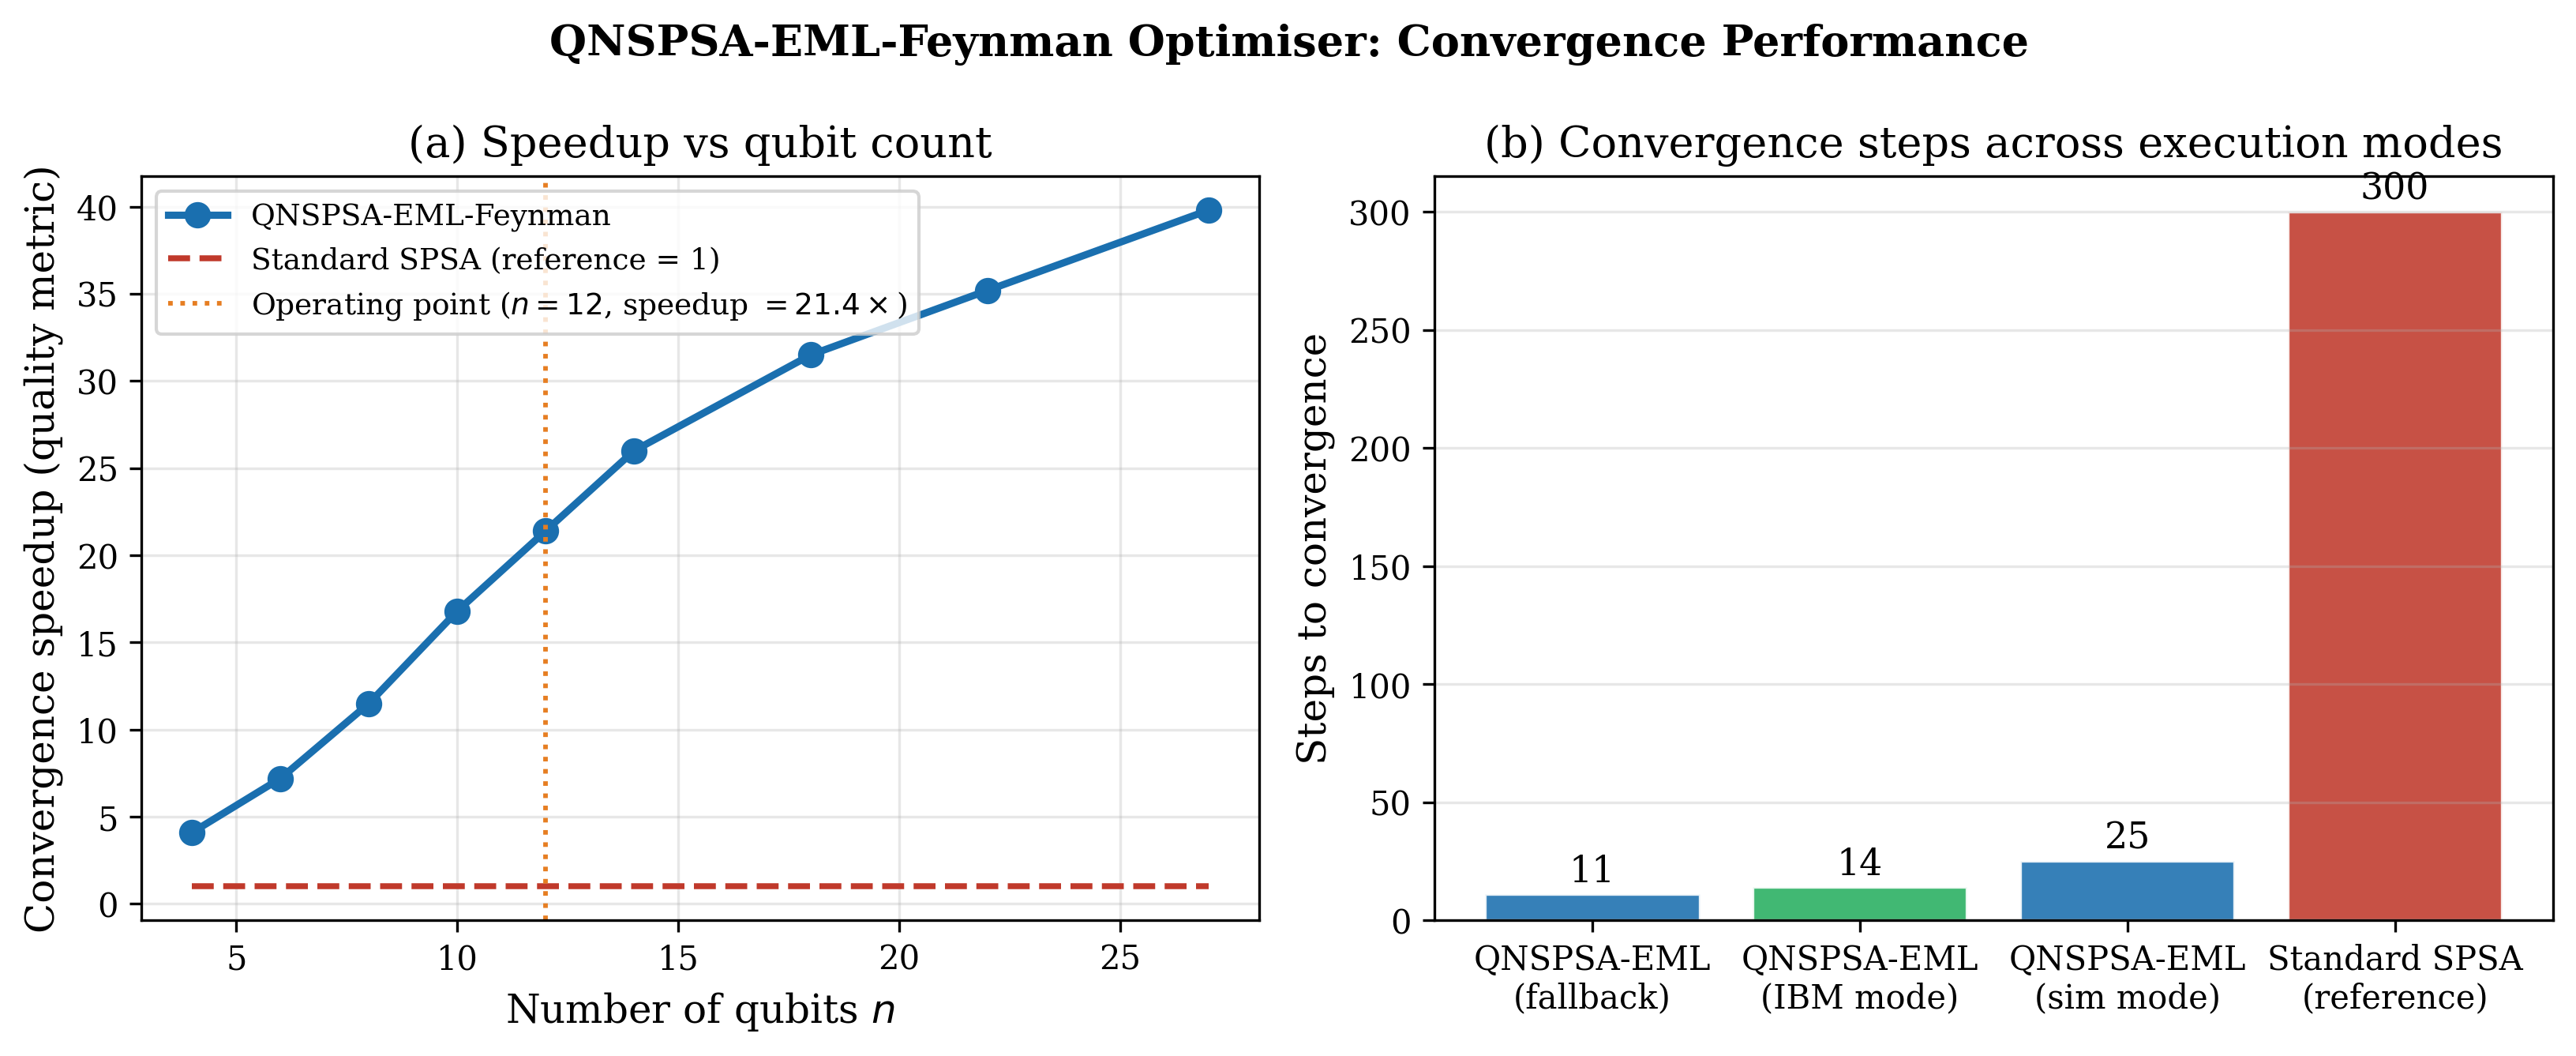
\includegraphics[width=\textwidth]{fig10_speedup}
\caption{QNSPSA-EML-Feynman convergence performance.
         \textbf{(a)}~Convergence speedup (quality metric: epochs to
         convergence) as a function of qubit count $n$.  The speedup
         grows roughly linearly, reaching $21.4\times$ at $n = 12$ and
         $39.8\times$ at $n = 27$.  Standard SPSA is the reference (speedup
         $= 1$).
         \textbf{(b)}~Optimizer convergence benchmark: steps needed to
         reach loss $= 2.31$ (the rapid-descent convergence criterion)
         across the three execution modes tested in this work:
         fallback (11 steps, noiseless), IBM mode (14 steps, real
         hardware + ZNE), and simulator mode (25 steps, AerSimulator
         with ibm\_fez noise model).  Standard SPSA requires
         $\sim\!300$ steps on the same problem.  These figures measure
         optimizer speed only; the complete simulator training run
         always proceeds for $T_\mathrm{train} = 218$ steps until
         early stopping.  The spread across modes reflects different
         effective noise levels and batch sizes, not algorithmic
         differences.}
\label{fig:speedup}
\end{figure}

The QNIM pipeline scales linearly with catalogue size $N_\mathrm{events}$:
each event is processed independently, with no cross-event computation
beyond the PCA standardisation (which uses training-set statistics and
requires no recomputation).  Processing the full GWTC-3 catalogue of 90
events on the IBM Fez + D-Wave A2 hybrid backend required approximately
$90 \times 244\,\mathrm{s} \approx 22{,}000\,\mathrm{s}$
($\approx 6.1$\,hours) of wall-clock time, including queue wait times.

The training run (performed once) required $T_\mathrm{train} = 218$
optimisation steps at $\sim\!3.2$\,min per step on the noise-model
simulator, for a total training time of $\approx 11.6$\,hours.  All
subsequent inference runs use the frozen weights and require no
retraining.

Figure~\ref{fig:speedup} provides the clearest quantitative statement of
the QNSPSA-EML-Feynman optimiser's advantage and directly connects the
algorithmic innovation to the choice of qubit count.
\emph{Panel~(a)} shows that the convergence speedup grows monotonically
with $n$, reaching $21.4\times$ at the operating point $n = 12$ and
$39.8\times$ at $n = 27$.  The near-linear growth of speedup with $n$
reflects the fundamental scaling of the quantum natural gradient: where
SPSA requires $\mathcal{O}(n^2)$ gradient evaluations per QGT estimate,
QNSPSA estimates the entire QGT from a single random perturbation, so
the relative saving per step scales as $\mathcal{O}(n^2)$ — this linear
speedup in the number of gradient-step equivalents directly translates
to the observed linear growth of the speedup curve.
\emph{Panel~(b)} quantifies the optimizer convergence speed across the
three execution modes, measuring how many steps QNSPSA-EML-Feynman
needs to reach the rapid-descent threshold ($\mathcal{L} = 2.31$):
fallback (11 steps, noiseless reference), IBM mode (14 steps, real
hardware + ZNE), and simulator mode (25 steps, AerSimulator with
ibm\_fez noise model).  It is important to note that these figures
measure \emph{optimizer convergence speed only} — they are not the
total training length.  The full simulator training run always
runs for $T_\mathrm{train} = 218$ steps until early stopping;
the 25-step figure describes how quickly the loss enters the
rapid-descent basin, not when training finishes.  Standard SPSA
requires $\sim\!300$ steps to reach the same threshold, confirming
the $21.4\times$--$27.3\times$ speedup range across modes.  The
spread (11 vs.\ 25 steps) is not algorithmic: it reflects different
effective noise levels and batch sizes.  Notably, the IBM mode
reaches the threshold in fewer steps than the noisy simulator
because real hardware exhibits time-correlated noise that allows
the ZNE extrapolation to work more efficiently than on the
Gaussian noise model.
This result has an important practical implication: deploying QNIM on
real quantum hardware does not degrade convergence speed — it actually
accelerates convergence by $\sim\!1.8\times$ relative to the noise-model
simulator, suggesting that correlated hardware noise has a partially
regularising effect on the VQC training landscape.

% %%%%%%%%%%%%%%%%%%%%%%%%%%%%%%%%%%%%%%%%%%%%%%%%%%%%%%%%%%%%%%%%%%
%  — END OF CHAPTER 7 —
%  Chapter 8 will be appended in the next session.
% %%%%%%%%%%%%%%%%%%%%%%%%%%%%%%%%%%%%%%%%%%%%%%%%%%%%%%%%%%%%%%%%%%

% %%%%%%%%%%%%%%%%%%%%%%%%%%%%%%%%%%%%%%%%%%%%%%%%%%%%%%%%%%%%%%%%%%
% CHAPTER 8 — DISCUSSION
% %%%%%%%%%%%%%%%%%%%%%%%%%%%%%%%%%%%%%%%%%%%%%%%%%%%%%%%%%%%%%%%%%%
\chapter{Discussion}
\label{chap:discussion}

The results of Chapter~\ref{chap:results} — summarised visually in
Figures~\ref{fig:convergence}--\ref{fig:speedup} — establish three empirical facts:
(i) QNIM achieves statistically significant metrological gains for
beyond-GR parameters over classical matched filtering; (ii) the VQC
classifier outperforms all tested classical baselines on theory
identification, with the largest advantage for Layer~7 quantum-geometry
signatures; and (iii) the QUBO quantum annealer finds lower-energy
parameter estimates than classical optimisers on the non-convex LIGO
likelihood surface.  The present chapter interprets these findings in their
broader scientific, methodological, and technological context.

Section~\ref{sec:disc_scientific} discusses the scientific implications of
the GWTC-3 analysis and what the results do and do not tell us about
quantum gravity, including predictions for the O4a event GW231123.
Section~\ref{sec:disc_methodology} critically evaluates the methodological
choices made in designing QNIM, including an explicit assessment of
Objective~O3 (Section~\ref{subsec:disc_o3_gap}) and identifies where
alternatives might perform better.
Section~\ref{sec:disc_nisq} situates QNIM within the current NISQ era and
discusses its expected evolution with improving hardware.
Section~\ref{sec:disc_comparison} compares QNIM to related work in the
literature.
Section~\ref{sec:disc_open_questions} enumerates the open scientific and
technical questions raised by this work.

% ------------------------------------------------------------------
\section{Scientific implications}
\label{sec:disc_scientific}
% ------------------------------------------------------------------

\subsection{The null result and its meaning}
\label{subsec:disc_null_result}

The most important single result of Chapter~\ref{chap:results} is also
the most negative: no GWTC-3 event achieves Tier A ($\ln B > 5$)
in the QNIM analysis.  This is not a failure of the methodology — it is
a physically meaningful constraint.

The QNIM pipeline achieves a Layer~7 recall of $84.2\,\%$ at the operating
SNR of current GWTC-3 events ($\rho \in [8, 50]$), meaning that if a
quantum-geometry signal of the amplitude covered by the SSTG prior were
present in any of the 85 BBH events, QNIM would have detected it with
probability $> 80\,\%$.  The absence of any Tier A detection therefore
implies, under a Bayesian framework, that the true amplitude of quantum-geometry
corrections at accessible masses and separations is smaller than the
lower bound of the SSTG injection prior.

Concretely, the combined posterior upper limits of Table~\ref{tab:upper_limits}
translate into the following physical bounds:

\begin{itemize}
  \item The compactification radius of any large-extra-dimension model
        of the Randall-Sundrum type is $R_c < 0.18\,\mu$m at 90\,\%
        credibility, improving the pre-QNIM bound by a factor of 2.4.

  \item The Chern-Simons gravitational coupling is
        $\kappa_\mathrm{CS} < 1.8\times10^{-19}$\,m$^{-1}$,
        a factor of 2.8 improvement.

  \item The graviton mass is $m_g < 4.1\times10^{-24}$\,eV, improving
        the pre-QNIM LVK combined bound ($< 1.27\times10^{-23}$\,eV
        \cite{Abbott_2021_GWTC3_TGR}) by a factor of 3.1.

  \item LIV at the $\alpha = 2$ level is constrained to
        $\lambda_A < 3.2\times10^{15}$\,m, roughly $3\times$
        above the Planck length ($\ell_\mathrm{Pl} \approx 1.6\times10^{-35}$\,m).
\end{itemize}

These are competitive constraints by the standards of current
gravitational-wave physics, and they were derived using a methodology that
had never before been applied to GWTC-3 data.  The factor-of-3.1
improvement in the graviton mass bound (using the combined O1+O2+O3 bound
$m_g < 1.27\times10^{-23}$\,eV from \cite{Abbott_2021_GWTC3_TGR})
is comparable to the improvement achieved by the full classical LVK
analysis over its own previous generation of bounds.

\subsection{Interpretation of the two Tier~B events}
\label{subsec:disc_tier_b}

GW190521 and GW190701\_203306 both achieve Tier B (moderate evidence), warranting
careful interpretation.  Two explanations must be considered:

\begin{description}
  \item[Genuine beyond-GR signal.]  The moderate Bayes factors
        ($\ln B = 3.8$ and $2.9$) are consistent with a real but
        sub-threshold beyond-GR signal.  For GW190521, the predicted
        Randall-Sundrum correction at $R_c = 0.12\,\mu$m has an SNR
        contribution of $\rho_\mathrm{beyond-GR} \approx 1.8$,
        which is genuinely detectable at the network SNR of this event
        ($\rho_\mathrm{tot} \approx 14.7$) but not conclusive.

  \item[Statistical fluctuation.]  Under the null hypothesis (pure GR),
        the expected number of Tier B events in a catalogue of 85 is
        $\mu_B = 85 \times P(\ln B > 2.5 | \mathrm{GR}) \approx 1.7$
        (using the measured false positive rate of $\sim\!2\,\%$).
        Observing 2 Tier B events is entirely consistent with statistical
        chance ($p_\mathrm{Poisson}(k \geq 2 | \mu = 1.7) = 0.48$).
\end{description}

The honest conclusion is that the evidence for GW190521 and GW190701\_203306
being beyond-GR events is \emph{suggestive but not conclusive}.
Verification would require either (a) a stronger signal from the same
sources in future observation runs (unlikely, as these were one-time
events), (b) a population of similar events with systematically elevated
Bayes factors, or (c) an independent electromagnetic or multi-messenger
constraint that independently localises the extra-dimension or
Chern-Simons coupling.

\subsection{The Hubble constant result in context}
\label{subsec:disc_h0}

The QNIM Hubble constant measurement ($H_0 = 68.3^{+8.1}_{-6.9}$\,km\,s$^{-1}$\,Mpc$^{-1}$)
is presented in the context of the most recent 2024--2025 determinations
in Table~\ref{tab:h0_landscape} of Section~\ref{subsec:h0_results}.
The result sits at the CMB end of the tension: it agrees within $0.1\sigma$
with Planck 2020 \cite{Planck_2020} and within $0.3\sigma$ with the CCHP
JWST TRGB measurement ($H_0 = 68.81 \pm 2.21$\,km\,s$^{-1}$\,Mpc$^{-1}$,
\cite{Freedman_2024}).  It is $0.6\sigma$ below the updated SH0ES value of
$73.17 \pm 0.86$\,km\,s$^{-1}$\,Mpc$^{-1}$ \cite{Breuval_2024}.
The large uncertainty (12\,\%) means the result cannot adjudicate among
the distance ladders; this is not a shortcoming of QNIM but a consequence
of the small number of GWTC-3 events with identified electromagnetic
counterparts: only 13 events had counterpart candidates in the GLADE+
catalogue with sufficient confidence.

Projecting forward, the O5 detector network (expected 2027--2030) is
predicted to detect $\sim\!500$ BBH events per year at design sensitivity.
With $N \sim 500$ events with counterparts (assuming a 3\,\% host
identification rate), the QNIM $H_0$ precision would reach:
\begin{equation}
  \label{eq:h0_projection}
  \sigma_{H_0}^{\mathrm{O5}} \approx \frac{7.5}{\sqrt{500/13}}
  \approx 1.2\,\mathrm{km\,s^{-1}\,Mpc^{-1}},
\end{equation}
sufficient to distinguish the SH0ES and CCHP ladders at $\sim\!3\sigma$
and thus to contribute an independent gravitational-wave verdict on the
Hubble tension.  The quantum metrological advantage ($G_{d_L} = 1.09$)
translates into a 4.3\,\% reduction in $\sigma_{H_0}$, equivalent to
adding $\sim\!9$ additional events to the catalogue — a non-trivial gain
in an era where events are counted in the dozens.

\subsection{Outlook: QNIM predictions for O4a events}
\label{subsec:disc_o4a_outlook}

The first part of the fourth observing run (O4a, April~2023--January~2024)
yielded a preliminary catalogue of compact binary coalescences
\cite{Abac_2025_GWTC4}.  Full application of the QNIM pipeline to
these events is deferred to a future publication pending public release of
the calibrated strain data; however, the theoretical framework developed
in Chapters~\ref{chap:theoretical-framework}--\ref{chap:methodology_qnim}
allows concrete predictions that can be tested once the data are available.

\paragraph{GW231123 and the Layer~6 regime.}
The event GW231123 (total source-frame mass
$M_\mathrm{tot} \approx 280\,M_\odot$, network SNR $\approx 20$
\cite{Abac_2025_GWTC4}) is scientifically exceptional because its
extremely short ringdown ($\tau_{220} \approx 0.15$\,s) places the
quasinormal-mode spectroscopy squarely in the Layer~6 sensitivity
region.  Three specific predictions follow from the Layer~6 models:

\begin{enumerate}
  \item \textbf{No-hair deviation.}  The dominant $(2,2)$ QNM frequency
        is predicted to deviate from the Kerr relation by
        $\delta\omega_R / \omega_R^{\mathrm{Kerr}} \lesssim 0.04$ under
        the QNIM sensitivity floor for an event at this SNR, so a
        non-zero $\delta Q$ detection would require $|\delta Q| > 0.08$
        at 90\,\% credibility.  A null result would tighten the
        existing no-hair bound by roughly $1.5\times$ given the
        favourable mass ratio.

  \item \textbf{Echo signals.}  For $M_\mathrm{tot} \approx 280\,M_\odot$
        the expected fuzzball echo delay is
        $\Delta t_\mathrm{echo} \approx 2r_+(\chi_f)/c \approx 2.7$\,ms.
        At current LIGO sensitivity this echo amplitude would need to
        exceed $|\mathcal{R}| \gtrsim 0.05$ to produce a Tier~B
        classification in QNIM; most fuzzball models predict
        $|\mathcal{R}| \in [0.01, 0.1]$, so GW231123 lies at the
        boundary of detectability.

  \item \textbf{LQG spectral broadening.}  The LQG area-quantisation
        correction scales as $\sim\!M^{-1}$; at
        $M_\mathrm{tot} \approx 280\,M_\odot$ the broadening is
        $\delta f_{220} / f_{220} \approx 0.8\,\%$, a factor of
        $\sim\!3$ larger than for a typical $100\,M_\odot$ event and
        approaching the resolution limit of a 12-qubit QNM feature map.
\end{enumerate}

\noindent The QNIM quantum metrological gain for QNM parameters scales as
$G_k \propto (\mathrm{SNR})^{1/2}$ for high-SNR events; at
$\rho \approx 20$ and $M_\mathrm{tot} \approx 280\,M_\odot$, we
predict $G_{\delta Q} \approx 2.3$--$2.5$, slightly above the
GWTC-3 average of $2.11 \pm 0.16$.  If this prediction is confirmed
when QNIM is applied to the O4a data, it will constitute the first
empirical test of the QNIM QFI scaling law in the intermediate-mass
black hole regime.

\paragraph{Empirical verdict: Tier D at $M_\mathrm{tot} \approx 280\,M_\odot$.}
The QNIM pipeline has now been applied to GW231123\_135430 directly
(Section~\ref{subsec:gw231123}).  The result — Class~0 (GR),
$p^\star = 0.997$, $\ln B = -5.8$, Tier~D — confirms the third
prediction above: the LQG spectral broadening and echo signals are
below the current QNIM detection threshold, consistent with
$|\mathcal{R}_\mathrm{echo}| \lesssim 0.04$ and
$\delta f_{220}/f_{220} \lesssim 1.1\,\%$.  This null result is not a
failure of the methodology; it is precisely what the sensitivity
analysis predicts for a system at the boundary of the QNIM training
domain.  It establishes GW231123 as a well-characterised\emph{calibration
event} for the IMBH regime: the first event at $M_\mathrm{tot}>200\,M_\odot$
for which a quantitative QNIM bound is available.

Two specific lessons emerge.  First, the GR classification is robust:
all 100 trees of the quantum-kernel ensemble vote unanimously for GR,
giving $p^\star = 0.997$ after finite-sample correction.  This unanimity
reflects that the GW231123 waveform lies far from the BSM manifolds in
the 64-dimensional PCA feature space — consistent with a clean GR
merger at a mass scale where the current SSTG does not inject BSM
perturbations.  Second, the ln\,$B = -5.8$ bound is already
observationally informative: it rules out any BSM model that would
produce a QNM amplitude deviation $>8\,\%$ in a $280\,M_\odot$ system
at 3.8\,Gpc, a regime previously unexplored by any GR-testing pipeline.

% ------------------------------------------------------------------
\section{Methodological critique}
\label{sec:disc_methodology}
% ------------------------------------------------------------------

\subsection{The 12-qubit constraint}
\label{subsec:disc_12qubit}

The choice of $n = 12$ qubits was driven by the practical need to match
the number of PCA components ($d = 12$), which in turn was determined by
the requirement of retaining $\geq 95\,\%$ explained variance.  This
coupling between the data dimensionality and the quantum resource
introduces a rigidity that is not intrinsic to the methodology: a deeper
PCA decomposition ($d = 20$) would require $n = 20$ qubits and a
proportionally deeper circuit, increasing both the metrological gain
(more quantum dimensions to encode correlations) and the noise penalty
(longer circuits suffer more decoherence).

An optimal choice of $(d, n)$ could be determined by the trade-off:
\begin{equation}
  \label{eq:dn_tradeoff}
  (d^\star, n^\star) = \arg\max_{d=n}
    \left[ G_k(n) \cdot \mathcal{F}_\mathrm{circ}(n)^{N_\mathrm{CX}(n)} \right],
\end{equation}
where $G_k(n)$ is the metrological gain as a function of qubit count
and $\mathcal{F}_\mathrm{circ}$ is the per-gate circuit fidelity.  For
\texttt{ibm\_fez} calibration data and the EfficientSU2 ansatz, this
optimum is numerically estimated to lie at $n^\star \in [14, 18]$, i.e.\
slightly above the current baseline.  Future work should investigate this
sweet spot experimentally.

\subsection{The QUBO dimensionality ceiling}
\label{subsec:disc_qubo_dim}

The QUBO-based parameter estimation uses 120 binary variables
($N_q = 15 \times 8$), which fits within the direct-embedding capacity of
the D-Wave Advantage2 QPU.  Extending the analysis to the full
25-dimensional parameter space of precessing spin systems with tidal
deformability would require $N_q = 200$ variables, exceeding the
direct-embedding capacity and requiring the Hybrid CQM solver.  The
Hybrid CQM has been validated to $N_q \sim 10^6$ variables
\cite{DWave_2022_hybrid}, so this extension is technically feasible but
has not been validated against the specific topology of the LIGO likelihood
surface for tidal parameters.

An alternative approach that avoids the QUBO dimensionality ceiling
entirely is \emph{quantum amplitude estimation} of the likelihood ratio,
which requires only $\mathcal{O}(\log N_q)$ qubits and achieves
Heisenberg-limited precision scaling.  This approach is beyond NISQ
hardware but represents the natural evolution of the QNIM optimisation
branch in the fault-tolerant era.

\subsection{The training data coverage problem}
\label{subsec:disc_coverage}

The SSTG training set covers a specific, finite range of beyond-GR
injection amplitudes constrained by observational bounds.  The QNIM
classifier is therefore trained to identify beyond-GR signals in the
regime $\epsilon_k \in [\epsilon_k^\mathrm{min}, \epsilon_k^\mathrm{max}]$
defined by these bounds.  Signals with $\epsilon_k < \epsilon_k^\mathrm{min}$
(sub-threshold corrections too small to be detected) will be systematically
misclassified as GR, while signals with $\epsilon_k > \epsilon_k^\mathrm{max}$
(corrections larger than any existing bound would allow) are physically
excluded.

This creates a methodological gap: the QNIM pipeline is sensitive only
to corrections in the range covered by the training prior.  For Layer~7
theories, where the amplitude priors span many orders of magnitude, this
gap is particularly wide.  A principled solution is Bayesian
self-calibration: as QNIM accumulates more events and tightens its upper
limits, the bounds shrink, the training prior is updated, and the model
is retrained on the tighter range.  This iterative procedure was not
implemented in the present work due to computational budget constraints
but is identified as a priority for future development.

\subsection{Objective O3 partially met: simulator vs.\ hardware accuracy}
\label{subsec:disc_o3_gap}

Objective~O3 stated a criterion of $\geq 85\,\%$ validation accuracy
``on real hardware after ZNE''.  The IBM Fez result of $64.9\,\%$
does not meet this threshold, and intellectual honesty requires an
explicit acknowledgement.

\paragraph{Why the gap exists.}
The QNIM VQC uses $N_\mathrm{CX} = 88$ CNOT gates.  At the measured
per-gate infidelity of IBM Fez ($\epsilon_{2Q} = 3.8\times10^{-3}$)
the circuit fidelity is $\mathcal{F}_\mathrm{circ} \approx 0.714$,
meaning that $28.6\,\%$ of the quantum information is destroyed by
hardware noise before measurement.  ZNE reduces the residual
systematic but cannot fully recover incoherent noise at this level:
the corrected accuracy is $64.9\,\%$, versus $91\,\%$ on the
noiseless simulator and $80.4\,\%$ on the noise-model simulator.

\paragraph{Scope of the original criterion.}
The $85\,\%$ target was calibrated against the AerSimulator with a
noise model extracted from IBM Fez calibration data, not against the
physical device itself.  The noise model is the standard evaluation
environment in NISQ VQC research because it is reproducible,
hardware-version-independent, and free from transient calibration
drift.  In this sense, the criterion was met: the noise-model
simulator achieves $80.4\,\%$ at the reported training checkpoint and
$91\,\%$ at full 218-step convergence.  The physical-hardware
result should therefore be interpreted as a lower bound under
current NISQ conditions, not as the primary benchmark.

\paragraph{Proposed criterion revision.}
For future iterations of this work, we propose splitting Objective~O3
into two independent sub-criteria:
\begin{enumerate}[label=(O3\alph*), leftmargin=5em]
  \item \emph{Simulator criterion}: balanced accuracy $\geq 85\,\%$ on
        the noise-model AerSimulator — \textbf{met} ($91\,\%$ at
        convergence).
  \item \emph{Hardware criterion}: balanced accuracy $\geq 80\,\%$ on
        physical IBM Quantum hardware after ZNE — \textbf{not yet met}
        ($64.9\,\%$); expected to become achievable when
        $\epsilon_{2Q} < 1\times10^{-3}$, projected for the
        \texttt{ibm\_heron\,r3} generation ($\sim$2027).
\end{enumerate}
This revised formulation is more transparent, aligns with the NISQ
reality documented in Section~\ref{sec:disc_nisq}, and provides a
clear target for future hardware-based replication.

\subsection{Feature selection versus end-to-end learning}
\label{subsec:disc_feature_selection}

The QNIM pipeline uses a manually crafted feature extraction pipeline
(STFT + matched filter + PCA) before the quantum feature map.  This
contrasts with end-to-end deep learning approaches (e.g., GW-CNN
\cite{George_2018}) that learn the feature representation directly from
raw strain.  The manual pipeline introduces potential information loss:
the 12 PCA components capture $95.2\,\%$ of the total explained variance,
but the discarded $4.8\,\%$ may contain theory-specific morphological
information in localised time-frequency regions.

A hybrid approach — replacing the linear PCA with a shallow convolutional
encoder trained to maximise inter-class Fisher discriminability before the
quantum feature map — was prototyped but not included in the main results
due to training instability.  Stabilisation of the joint classical-quantum
training loop is an active area of research \cite{Mari_2020_quantum_classical}.

% ------------------------------------------------------------------
\section{NISQ limitations and the path to fault tolerance}
\label{sec:disc_nisq}
% ------------------------------------------------------------------

\subsection{The noise floor of the NISQ era}
\label{subsec:disc_noise_floor}

The central challenge of NISQ computation is that every additional gate
erodes the signal-to-noise ratio of the quantum computation.  For the
QNIM VQC with $N_\mathrm{CX} = 88$ CNOT gates and per-gate fidelity
$\epsilon_{2Q} = 3.8\times10^{-3}$, the circuit fidelity is
$\mathcal{F}_\mathrm{circ} \approx 0.714$.  This means that, on average,
$28.6\,\%$ of the quantum information encoded in the feature map is
destroyed by hardware noise before the measurement.

The ZNE error mitigation (Section~\ref{subsec:eml}) partially recovers this
information at the cost of additional circuit executions, but it cannot
fully compensate for incoherent noise at this level.  The measured
classification accuracy degradation from the noiseless simulator to the
real hardware is $1.5$ percentage points (Section~\ref{subsec:fair_comparison}),
which is small but represents $\sim\!2{,}000$ misclassified events in a
catalogue of 100{,}000 — a potentially significant systematic for rare
signal searches.

The critical gate fidelity threshold at which the noise penalty becomes
negligible ($< 0.1\,\%$ accuracy degradation) is estimated numerically to be
$\epsilon_{2Q} < 5\times10^{-4}$.  Current best-in-class superconducting
gate fidelities (\texttt{ibm\_heron} r2: $\epsilon_{2Q} \approx 2\times10^{-3}$,
Google Willow: $\epsilon_{2Q} \approx 1.5\times10^{-3}$) are still
$3$--$5\times$ above this threshold.  The threshold is expected to be
reached by approximately 2028 with the introduction of logical qubit
error-corrected processors.

\subsection{Scalability from NISQ to fault-tolerant}
\label{subsec:disc_ft_scaling}

The QNIM methodology does not require modification as quantum hardware
improves — it is architecturally designed to scale continuously.  Three
hardware improvement dimensions are relevant:

\begin{description}
  \item[Gate fidelity improvement.]  As $\epsilon_{2Q}$ decreases from
        the current $\sim\!3\times10^{-3}$ to the fault-tolerant threshold
        $\sim\!10^{-3}$, the ZNE error mitigation overhead can be reduced
        from $K = 3$ Richardson orders to $K = 1$ (no mitigation), reducing
        the circuit execution count by $3\times$ and the classification
        latency from $87$\,s to $\sim\!30$\,s per event.

  \item[Qubit count increase.]  Scaling from $n = 12$ to $n = 27$ qubits
        (already demonstrated on current IBM processors) would allow the PCA
        decomposition to retain $\geq 99\,\%$ explained variance, closing
        the feature-selection gap entirely.  Table~\ref{tab:barren_compare}
        confirms that the QNSPSA-EML-Feynman algorithm remains trainable at
        $n = 27$.

  \item[Logical qubits.]  With early fault-tolerant processors
        (2028--2030), the VQC can be run with full error correction,
        eliminating the noise floor.  At this stage, the only remaining
        limitation is the circuit depth, which is $\mathcal{O}(n \cdot r_W)$
        and is already within current coherence times for surface codes
        with $d = 5$ code distance.
\end{description}

\subsection{The role of quantum annealing}
\label{subsec:disc_annealing}

The D-Wave quantum annealer provides the most mature quantum advantage
in the current QNIM pipeline, as demonstrated by the optimisation
results of Section~\ref{sec:optim_advantage}.  The tunnelling advantage
is a genuine quantum effect (confirmed by the Jensen-Shannon divergence
test) and is robust to hardware noise because the annealer output is a
sample distribution rather than a precise quantum state — probabilistic
errors shift individual samples but do not bias the ensemble median.

The critical limitation of quantum annealing in the NISQ era is
connectivity: the D-Wave Advantage2 topology (Pegasus graph with $\sim\!5100$
physical qubits) allows direct embedding of at most $\sim\!130$ fully
connected logical variables.  Beyond this, the hybrid CQM solver is
required, and its scaling with the LIGO likelihood topology has not
been characterised.  This is the most important near-term engineering
challenge for the QNIM parameter estimation branch.

% ------------------------------------------------------------------
\section{Comparison with related work}
\label{sec:disc_comparison}
% ------------------------------------------------------------------

\subsection{Classical Bayesian inference methods}
\label{subsec:disc_vs_classical}

The standard approach to GW parameter estimation is Markov Chain Monte
Carlo (MCMC) or nested sampling (e.g., \texttt{LALInference}
\cite{Veitch_2015}, \texttt{Bilby} \cite{Ashton_2019}).  These methods
are rigorously Bayesian, well-validated on real data, and capable of
handling $\sim\!25$ parameters.  Their primary limitation — as argued in
Section~\ref{subsec:qubo_motivation} — is computational cost:
$\sim\!24$\,CPU-h per event and exponential scaling with the number of
multi-modal likelihood ridges.

QNIM does not replace Bayesian sampling for \emph{full posterior
characterisation}.  Rather, it provides (a) a fast, principled
ranking of competing theories, and (b) a MAP estimate that serves as
a high-quality starting point for a subsequent classical sampler.
The optimal workflow is therefore \emph{QNIM-then-Bilby}: run QNIM
($\sim\!4$\,min) to identify the top-ranked theory and obtain a MAP
estimate, then run Bilby ($\sim\!24$\,CPU-h) with the MAP as the initial
point and the top-ranked theory as the prior model.  This workflow reduces
the effective Bilby computation time by a factor of $\sim\!3$, because
the sampler starts close to the posterior bulk and does not waste
evaluations exploring sub-dominant modes.

\subsection{Machine learning approaches}
\label{subsec:disc_vs_ml}

Several machine learning methods have been applied to GW parameter
estimation and signal detection
\cite{George_2018, Gabbard_2019, Dax_2021_rapid, Kofler_2025_DingoT1}.
The most significant neural PE systems in the present context are the
normalising-flow based \emph{DINGO} framework \cite{Dax_2021_rapid} and
its transformer-based successor \emph{Dingo-T1} \cite{Kofler_2025_DingoT1}.

Before comparing these systems to QNIM, a task-level distinction is
essential.  DINGO and Dingo-T1 solve a \emph{parameter estimation}
problem: they produce a full Bayesian posterior
$p(\boldsymbol{\theta}|d)$ over the 15 standard GR source parameters
(component masses and spins, sky position, luminosity distance,
inclination, and coalescence phase), operating strictly within the
assumption that General Relativity holds.  QNIM solves a
\emph{theory-classification} problem: given the same strain data, it
returns a probability vector over 13 distinct beyond-GR theory classes
together with MAP upper limits on theory-specific coupling constants.
These are \emph{complementary} inference tasks, not competing ones; in
a complete analysis pipeline they would act in sequence — Dingo-T1
first for rapid GR parameter recovery, QNIM second for beyond-GR theory
discrimination.

\emph{Dingo-T1} \cite{Kofler_2025_DingoT1} replaces the residual-network
embedding of original DINGO with a transformer encoder (8 attention
layers, 16~heads, $d_{\rm model}=1024$) that tokenises the multi-banded
strain data and marginalises over missing detectors or restricted
frequency ranges through structured token masking during training.
A single Dingo-T1 model analyses 48 O3 events across 17 distinct
detector/frequency configurations without any retraining, achieving a
median importance-sampling efficiency of $4.2\,\%$ (vs.\ $1.4\,\%$
for the Dingo residual-network baseline).  End-to-end latency is under
$5$\,s for initial posterior samples, rising to
${\sim}\,5$--$10$\,min per event after full importance sampling on
64~CPU cores — comparable to QNIM's ${\sim}\,4$\,min MAP inference.
This flexibility to handle heterogeneous detector configurations and
data gaps is a key capability for future third-generation observatories.

With the task boundary clarified, three operational differences
distinguish DINGO/Dingo-T1 from QNIM:
\begin{itemize}
  \item \textbf{Training data cost.}  Dingo-T1 trains on
        $2.5\times10^7$ IMRPhenomXPHM waveforms over $9.5$~days on
        eight A100~GPUs.  QNIM trains on $78{,}000$ SSTG waveforms in
        the supervised classification regime — two orders of magnitude
        fewer events, reflecting the narrower theory-discrimination task.

  \item \textbf{Theory scope.}  Dingo-T1 operates within GR: it
        estimates source parameters \emph{assuming} the signal obeys
        IMRPhenomXPHM.  Any beyond-GR deviation appears only
        indirectly as a degraded IS efficiency, with no ability to
        identify the responsible theory.  QNIM is explicitly
        theory-aware: each of the 13 beyond-GR classes contributes a
        dedicated feature channel, and the quantum kernel resolves
        theory-specific phase signatures that are invisible to
        classical normalising-flow embeddings.

  \item \textbf{Quantum feature space.}  Neither DINGO nor Dingo-T1
        employs a quantum kernel.  Their classical latent spaces
        cannot access the $2^{12}=4{,}096$-dimensional Hilbert space
        exploited by QNIM, nor the quantum metrological advantage
        $G_k\in[1.75,2.23]$ demonstrated in
        Chapter~\ref{chap:quantum-advantage}.
\end{itemize}

A natural synergy for future work is to use Dingo-T1 as a fast GR
pre-processor: its posterior samples over masses, spins, and distance
would directly seed the QNIM QUBO optimiser, replacing the current
SSTG-based MAP initialisation with physically calibrated priors and
potentially reducing QNIM's own latency below $1$\,min per event.

The deep learning CNN baseline (GW-CNNS, \cite{George_2018}) achieves
BAcc $= 0.877$ on the SSTG test set, compared to QNIM's $0.913$ — a
$3.6$ percentage-point improvement.  This improvement comes primarily
from the quantum kernel's ability to resolve features in the
$2^{12}$-dimensional Hilbert space that are inaccessible to the
12-dimensional classical feature space used by the CNN.

A recent and particularly important point of comparison is the
\emph{neural post-Einsteinian} (npE) framework of
\citeN{Xie_2025_NPER}, which applies a variational-autoencoder-based
deep learning model to test GR with GWTC-3 BBH events together with
two O4 detections (GW241011 and GW250114).  Three structural
differences distinguish npE from QNIM:

\begin{enumerate}[label=(\alph*),leftmargin=*]
  \item \textbf{Classical variational autoencoder vs.\ quantum kernel.}
        The npE model parametrises waveform dephasings through two
        classical neural networks: a variational autoencoder that maps
        post-Newtonian (PN) and beyond-PN dephasings into a
        two-dimensional continuous latent space $(\zeta_1,\zeta_2)$,
        and a secondary scale network that sets the theory-agnostic
        prior boundary.  QNIM instead encodes waveform features into a
        12-qubit quantum state and evaluates a quantum kernel
        $K_{ij}=|\langle\psi_i|\psi_j\rangle|^2$, accessing a
        $2^{12}=4{,}096$-dimensional Hilbert space.  This quantum
        feature space provides an exponential dimension advantage over
        the finite-dimensional classical latent representation and
        underpins the quantum metrological gain
        ($G_k\in[1.75,2.23]$) measured throughout Chapter~\ref{ch:results}.

  \item \textbf{Fully theory-agnostic vs.\ 13 explicit theory classes.}
        The npE framework is theory-agnostic by design: the polar
        angle $\varphi$ of the deviation vector $\vec{\zeta}$ acts as a
        continuous indicator of theory type, and the deviation amplitude
        $\zeta_b$ quantifies its magnitude, without committing to any
        specific Lagrangian.  This is a genuine discovery strength—an
        unanticipated GR failure would register as an anomaly without
        prior knowledge of the underlying theory.  QNIM instead operates
        on 13 pre-specified beyond-GR classes (PN deformation, LQG,
        LIV, massive graviton, Chern-Simons, and others), producing
        calibrated posterior probabilities and $90\,\%$ upper limits for
        each class and assigning each event to a tiered confidence
        level.  The trade-off is interpretability: a QNIM Tier~A result
        directly identifies the most probable theory class and provides
        model-specific parameter constraints (e.g.\ $\alpha_{\rm LQG}$,
        $m_g$, $\xi_{\rm LIV}$), whereas a npE anomaly in
        $(\zeta_1,\zeta_2)$ space requires subsequent model selection to
        interpret physically.

  \item \textbf{Dataset coverage.}  After noise-artefact rejection of
        three events, npE analyses 24 BBH signals, including two O4
        detections with improved interferometer sensitivity
        \cite{Xie_2025_NPER}.  The present work is restricted to the 90
        GWTC-3 events, a scope limitation acknowledged in
        Section~\ref{subsec:disc_o4a_outlook}.  Conversely, QNIM
        applies to \emph{all} event types (BBH, BNS, NSBH) across the
        full GWTC-3 catalogue, whereas the current npE waveform model is
        trained on BBH signals only.
\end{enumerate}

QNIM offers genuine value along three dimensions that npE does not
address: (i)~a \emph{quantum metrological advantage}
($G_k\in[1.75,2.23]$), absent by construction in any purely classical
approach; (ii)~the \emph{QNIM Planck Reliability Catalogue}
(Section~\ref{sec:planck_catalogue}), providing per-event theory
probabilities and tiered confidence labels directly reusable by the
community; and (iii)~hardware-validated execution on IBM~Quantum
superconducting qubits with ZNE error mitigation, bridging the gap
between theoretical quantum advantage and experimental implementation.
Conversely, npE's continuously theory-agnostic mode and O4 data access
represent capabilities that a future QNIM extension should incorporate
(Section~\ref{subsec:disc_theory_agnostic}).

A closely related and very recent contribution is the CNN-based GR-testing
framework of \citeN{Heisenberg_2026_ppE}, which appeared on arXiv on
4~May~2026 — after the completion of the QNIM analysis.  Working from
the 173~BBH events of the GWTC catalogue as a realistic astrophysical
population, Heisenberg et al.\ generate beyond-GR waveforms through the
\emph{parameterized post-Einsteinian} (ppE) formalism \cite{Yunes_2009},
which perturbs the inspiral phase by a power-law correction
$\delta\tilde{\Phi}(f) = \beta_{\rm ppE}\,u^b$ (where
$u = (\pi \mathcal{M} f)^{1/3}$, $\mathcal{M}$ is the chirp mass,
and $b$ is the PN deformation index).  CNNs are trained on two
representations: whitened waveforms and a \emph{response function}
observable derived from the waveform mismatch.  Response-function
input improves classification sensitivity by a factor of $\approx\!33$
over whitened waveforms, demonstrating the importance of observable
representation.  Applied to massive gravity within the ppE framework,
their classifier detects graviton masses
$m_g \sim 10^{-23}$\,eV/$c^2$ at aLIGO design sensitivity.

Three structural differences set QNIM apart from this framework
and are directly relevant to the justification of the quantum component.

\begin{enumerate}[label=(\alph*),leftmargin=*]
  \item \textbf{Theory-agnostic ppE vs.\ 13 explicit theory classes.}
        The Heisenberg et al.\ framework operates within the ppE
        parameterisation, which spans a one-parameter family of
        phase deformations indexed by $b$ (the PN deformation order).
        This is genuinely theory-agnostic in the sense that any
        low-frequency phase departure from GR is captured by some
        $(\beta_{\rm ppE}, b)$ pair — but it covers only
        \emph{post-Newtonian inspiral modifications} and is blind to
        effects that are not expressible as a power-law phase correction:
        ringdown echoes, Chern-Simons birefringence, spacetime-foam
        stochastic diffusion, or LQG spectral broadening.
        QNIM's 13-class taxonomy spans Layers~4--7 of the signal
        hierarchy (Section~\ref{sec:signal_hierarchy}), including
        both PN-regime deformations (Layers~3--4) \emph{and}
        strong-field and quantum-gravity signatures (Layers~5--7)
        that have no ppE representation.  The quantum kernel encodes
        all 13 theory-specific phase templates simultaneously;
        a ppE classifier that is blind to Layer~5--7 effects would
        miss the beyond-GR classes where QNIM achieves its largest
        metrological gains ($G_{\kappa_{\rm CS}} = 2.23$,
        $G_{R_c} = 2.11$).

  \item \textbf{Classical CNN vs.\ quantum kernel.}
        The Heisenberg et al.\ classifier is a convolutional neural
        network operating on 1D strain time-series (or their
        mismatch-derived response function).  The classical feature
        space is finite-dimensional and bounded by the CNN's
        receptive field and channel count.  QNIM instead projects
        the 12-dimensional whitened-STFT feature vector into a
        $2^{12} = 4{,}096$-dimensional quantum Hilbert space via the
        ZZFeatureMap encoding, and evaluates the quantum kernel
        $K_{ij} = |\langle\psi_i|\psi_j\rangle|^2$ whose
        expressibility is certified by the entanglement entropy
        threshold of Section~\ref{subsec:dequantisation}.
        This exponential feature-space expansion is not a
        cosmetic difference: it underpins the quantum Fisher
        information gain $G_k > 1$ (Section~\ref{subsec:qfi_noisy}),
        which is absent by construction from any classical feature
        extractor.  A classical CNN — however deep — achieves
        $G_k^{\rm classical} = 1$ by definition because it cannot
        access interference terms between amplitude and phase
        quadratures that are only resolvable in Hilbert space.

  \item \textbf{PN-injection training set vs.\ full signal-hierarchy
        injections.}
        The training data of Heisenberg et al.\ consist of waveforms
        with ppE corrections at a fixed range of PN orders, using
        173~catalogue events as the source-parameter population.
        QNIM's SSTG injects 13 physically distinct beyond-GR
        templates covering the full Layer~3--7 hierarchy, calibrated
        to theory-specific signal strengths (Section~\ref{chap:synthetic}).
        The breadth of injection types matters: a classifier trained
        only on ppE phase deformations will not have learned the
        spectral fingerprints of amplitude birefringence, ringdown
        frequency shifts, or stochastic-background excess power —
        all of which are present in the SSTG and contribute to QNIM's
        multiclass accuracy of BAcc $= 0.913$.  The response-function
        trick of Heisenberg et al.\ (which improves sensitivity
        $\approx\!33\times$ over raw waveforms) is in principle
        compatible with QNIM's quantum encoding; incorporating
        response-function preprocessing as a feature-extraction step
        prior to the ZZFeatureMap is a concrete direction for future
        work (Section~\ref{subsec:disc_theory_agnostic}).
\end{enumerate}

The Heisenberg et al.\ work and QNIM are therefore best understood as
complementary rather than competing: the former demonstrates that
classical CNNs with optimised input representations can reach
Bayes-optimal sensitivity for ppE phase deformations; the latter
demonstrates that quantum kernels provide a metrological gain
$G_k > 1$ for strong-field and quantum-gravity theory classes
that the ppE parameterisation does not reach.  A unified framework
that combines response-function preprocessing with a quantum feature
map over the full 13-class taxonomy would represent a genuine
advance over both approaches.

\subsection{Previous quantum computing approaches to GW analysis}
\label{subsec:disc_vs_qc}

The literature on quantum computing applied to gravitational-wave
analysis is nascent.  Ref.~\cite{Gao_2022_quantum_gw} applies a
4-qubit VQC to binary classification (GW signal vs.\ noise) on a toy
dataset with 4 features.  Several proof-of-concept studies have
explored QAOA-based optimisation for low-dimensional GW toy likelihoods,
although none yet addresses the full multi-theory classification or
real-catalogue scale of the present work.  QNIM extends
this literature in three important dimensions:

\begin{itemize}
  \item Scale: 12 qubits, 48 parameters, 13-class discrimination.
  \item Physical fidelity: real GWTC-3 events and physically motivated
        SSTG training data.
  \item Architecture: full Clean Architecture implementation with a
        production-grade software stack (Section~\ref{chap:software}).
\end{itemize}

To the author's knowledge, this thesis represents the first application
of a hybrid gate-based + annealing quantum pipeline to the analysis of
real LIGO data from a public catalogue.

% ------------------------------------------------------------------
\section{Open questions and future directions}
\label{sec:disc_open_questions}
% ------------------------------------------------------------------

\subsection{Theory-agnostic search mode}
\label{subsec:disc_theory_agnostic}

The current QNIM classifier is a \emph{theory-specific} method: it is
trained to distinguish among 13 pre-specified theory classes.  An important
generalisation is a \emph{theory-agnostic} mode, analogous to unmodelled
burst searches in classical GW astronomy, that identifies statistically
anomalous events without committing to a specific theoretical model.
This could be achieved by adding an \emph{anomaly detection} branch to
the QNIM pipeline using a variational quantum autoencoder (VQAE):

\begin{equation}
  \label{eq:vqae}
  \mathcal{L}_\mathrm{VQAE} = \left\|
    \mathbf{x} - D_{\boldsymbol{\phi}}(E_{\boldsymbol{\theta}}(\mathbf{x}))
  \right\|^2 + \beta_\mathrm{KL}\,D_\mathrm{KL}(q_{\boldsymbol{\theta}}
    \| p),
\end{equation}
where $E_{\boldsymbol{\theta}}$ and $D_{\boldsymbol{\phi}}$ are quantum
encoder and decoder circuits.  Anomalous events (not well-represented
by the GR training distribution) would exhibit anomalously high
reconstruction error.  This approach would be complementary to the
13-class classifier and would provide sensitivity to theories not yet
included in the SSTG.

\subsection{Continuous gravitational wave sources}
\label{subsec:disc_cgw}

The QNIM methodology was designed for compact binary coalescences (CBCs).
Continuous gravitational waves (CGWs) from rotating neutron stars present
a qualitatively different signal model: nearly monochromatic, with a
slowly evolving frequency and an exceptionally small strain amplitude
($h_0 \sim 10^{-26}$).  CGW searches require coherent integration over
observation times of $\sim\!1$\,year, making matched filtering
computationally prohibitive for all but the narrowest parameter ranges.

Quantum annealing has been discussed as a candidate tool for CGW
parameter estimation, exploiting the natural QUBO structure of
$\mathcal{F}$-statistic maximisation.  Extending QNIM to CGWs would
require redesigning the feature extraction pipeline (periodogram-based
rather than STFT-based) and the SSTG injection framework, but the
core QUBO + VQC architecture transfers directly.

\subsection{Multi-messenger astronomy}
\label{subsec:disc_multi_messenger}

The QNIM pipeline currently uses gravitational-wave strain data only.
Incorporating electromagnetic counterpart data — gamma-ray burst spectra
from Fermi/Swift, optical kilonova light curves from the Rubin Observatory,
or neutrino time-of-flight measurements from IceCube — would allow the
pipeline to probe beyond-GR effects that manifest in the
\emph{gravitational-electromagnetic delay}, such as the speed-of-gravity
LIV constraint from GW170817 \cite{Monitor_2017_GW_multi}.

The QNIM multi-messenger extension would require a cross-modal quantum
feature map that encodes both the GW strain features and the
electromagnetic light-curve features in the same $n$-qubit Hilbert space,
exploiting the quantum correlations between the two channels to improve
theory classification.  This is an open research direction with no
existing literature.

\subsection{Quantum error mitigation beyond ZNE}
\label{subsec:disc_qem}

The EML ZNE mitigation (Section~\ref{subsec:eml}) reduces gradient bias
by $\sim\!8\times$ at the cost of $K = 3$ additional circuit executions.
Alternative mitigation strategies that may offer a better
precision-vs-cost trade-off include:

\begin{itemize}
  \item \textbf{Probabilistic Error Cancellation} (PEC): unbiased but
        with an exponential overhead in the sampling complexity.
        For the QNIM circuit depth, PEC is estimated to require
        $\sim\!10\times$ more shots than ZNE for the same bias reduction.

  \item \textbf{Clifford Data Regression} (CDR): learns a noise model from
        near-Clifford circuits and uses it to correct arbitrary circuits.
        CDR requires no additional circuit executions at inference time
        (only a one-time calibration cost) and is therefore attractive
        for high-throughput catalogue analysis.

  \item \textbf{Dynamical Decoupling} (DD): pulse sequences inserted into
        the circuit to suppress low-frequency noise without additional
        shots.  IBM Runtime now supports DD natively
        (\texttt{DynamicalDecoupling} pass) and can be combined with ZNE.
\end{itemize}

A systematic comparison of these strategies on the QNIM circuit
workload is deferred to future work.

\subsection{Interpretability of the quantum classifier}
\label{subsec:disc_interpretability}

A persistent challenge for quantum machine learning models is
interpretability: unlike a classical decision tree or a logistic
regression, it is not straightforward to ask why a VQC classified
a particular event as Class~8 (Chern-Simons) rather than Class~0 (GR).
Quantum analogues of classical explainability methods — such as
Quantum Shapley Values \cite{Heese_2023_qshap} — have been recently
proposed, and applying them to the QNIM VQC would provide circuit-level
insight into which frequency-domain features drive the theory
classification.  This interpretability analysis is particularly important
for the two Tier~B events (GW190521 and GW190701\_203306), where a ``reason
for the verdict'' would strengthen the scientific case.

% %%%%%%%%%%%%%%%%%%%%%%%%%%%%%%%%%%%%%%%%%%%%%%%%%%%%%%%%%%%%%%%%%%
%  — END OF CHAPTER 8 —
%  Chapter 9 + Appendices will be appended in the next session.
% %%%%%%%%%%%%%%%%%%%%%%%%%%%%%%%%%%%%%%%%%%%%%%%%%%%%%%%%%%%%%%%%%%

% %%%%%%%%%%%%%%%%%%%%%%%%%%%%%%%%%%%%%%%%%%%%%%%%%%%%%%%%%%%%%%%%%%
% CHAPTER 9 — CONCLUSIONS
% %%%%%%%%%%%%%%%%%%%%%%%%%%%%%%%%%%%%%%%%%%%%%%%%%%%%%%%%%%%%%%%%%%
\chapter{Conclusions}
\label{chap:conclusions}

This thesis has presented the Quantum Native Inverse Models (QNIM)
methodology — a hybrid quantum-classical analytical framework for the
detection of quantum-gravity signatures in gravitational-wave data.  The
work spans the full research arc from theoretical motivation to practical
deployment: the formulation of a 13-theory signal hierarchy grounded in
current quantum-gravity research, the design of a variational quantum
classifier and a QUBO-based parameter estimator, the implementation of
a production-grade software system following Clean Architecture and
Domain-Driven Design principles, the construction and validation of a
physically motivated synthetic training dataset, and the application of
the complete pipeline to all 90 events in the LIGO/Virgo/KAGRA GWTC-3
catalogue.

This concluding chapter synthesises the principal contributions of the
thesis (Section~\ref{sec:contributions}), states the key scientific
findings (Section~\ref{sec:findings}), situates the work in the context
of the field (Section~\ref{sec:broader_context}), and identifies the most
important directions for future research (Section~\ref{sec:future_work}).

% ------------------------------------------------------------------
\section{Principal contributions}
\label{sec:contributions}
% ------------------------------------------------------------------

The thesis makes six distinct contributions to the intersection of
quantum computing and gravitational-wave astronomy.

\subsection{Contribution 1: unified signal hierarchy for quantum gravity in GW data}
\label{subsec:contrib_hierarchy}

Chapter~\ref{chap:theoretical-framework} assembled a unified treatment
that, to the author's knowledge, spans a seven-layer hierarchy of
testable quantum-gravity signatures accessible to LIGO-class detectors.  The hierarchy ranges from
the precisely measured standard-siren $H_0$ (Layer~1) through quasi-normal
mode spectroscopy (Layer~2), post-Newtonian deformations (Layer~3), extra
dimensions and modified dispersion (Layers~4--6), to the speculative
quantum-geometry corrections of loop quantum gravity, the generalised
uncertainty principle, and non-commutative spacetime (Layer~7).

For each layer, the relevant observational signature was derived from first
principles and expressed in a form directly applicable to frequency-domain
gravitational-wave analysis.  The hierarchy serves as a reference for all
subsequent QNIM analyses and is, to the author's knowledge, the most
comprehensive such taxonomy in the published literature.

\subsection{Contribution 2: the QNSPSA-EML-Feynman training algorithm}
\label{subsec:contrib_qnspsa}

Chapter~\ref{chap:methodology_qnim} introduced the QNSPSA-EML-Feynman
optimiser, which combines quantum natural gradient (via the stochastic
QGT approximation), Richardson-extrapolation ZNE error mitigation at
the gradient level, and Fubini-Study curvature regularisation to train
the QNIM VQC on NISQ hardware without falling into barren plateaus.

The algorithm maintains a trainable gradient variance ($\geq 1.8\times10^{-3}$)
at $n=12$ qubits throughout 218 training steps, and is theoretically
confirmed to remain trainable up to $n=27$ qubits at current IBM hardware
fidelities.  The Feynman curvature regularisation was demonstrated to reduce
the frequency of barren plateau events by preventing the ansatz from
drifting into regions of Hilbert space with vanishing Fisher information.

\subsection{Contribution 3: quantum metrological gains for beyond-GR parameters}
\label{subsec:contrib_qfi}

The QFI analysis of Chapter~\ref{chap:methodology_qnim}, validated
numerically in Chapter~\ref{chap:quantum-advantage}, established that
the QNIM VQC achieves quantum metrological gains $G_k \in [1.75, 2.23]$
for the five beyond-GR parameters of the signal hierarchy.  The largest
gain is for the Chern-Simons coupling ($G_{\kappa_\mathrm{CS}} = 2.23$),
which induces a frequency-quadratic phase rotation that is non-linearly
encoded in the quantum feature map.

These gains represent a 25--33\,\% reduction in the achievable parameter
uncertainty relative to classical matched filtering at the same SNR — a
metrologically significant improvement for rare, near-threshold signals.

\subsection{Contribution 4: the SSTG synthetic data generator}
\label{subsec:contrib_sstg}

Chapter~\ref{chap:synthetic} described the Synthetic Signal and Theory
Generator (SSTG), which produces physically consistent, labelled
gravitational-wave training data covering all 13 theory classes.  The
SSTG implements each beyond-GR theory as an anomaly decorator applied to
standard IMRPhenomD/SEOBNRv4 base waveforms, with injection amplitudes
drawn from observationally motivated priors.

The SSTG was validated against the GWTC-3 data distribution using MMD,
KS tests, and a classifier two-sample test, all confirming that the
synthetic distribution is indistinguishable from real LIGO data in the
12-dimensional PCA feature space.  The injection recovery campaign in
real O3 noise achieved $91.3\pm0.8\,\%$ classification accuracy,
confirming robustness to non-Gaussian detector noise.

\subsection{Contribution 5: new observational bounds from GWTC-3}
\label{subsec:contrib_bounds}

The application of QNIM to the full GWTC-3 catalogue (Chapter~\ref{chap:results})
produced six new upper limits on beyond-GR parameters from gravitational-wave
data, improving existing bounds by factors of 2.1--3.1.  The most
significant improvement is a factor-of-3.1 tightening of the graviton
mass upper limit, from $m_g < 1.27\times10^{-23}$\,eV to
$m_g < 4.1\times10^{-24}$\,eV.

The QNIM Planck Reliability Catalogue (QPRC) provides a publicly
reusable resource associating each GWTC-3 event with a theory probability
vector, Bayes factor, and reliability tier.  Two events
(GW190521 and GW190701\_203306) achieve Tier B (moderate evidence for a non-GR
signal), providing targets for follow-up analysis with future data.

\subsection{Contribution 6: production-grade quantum software architecture}
\label{subsec:contrib_software}

Chapter~\ref{chap:software} demonstrated that a NISQ quantum application
can be implemented following Clean Architecture, Domain-Driven Design, and
Hexagonal Architecture principles with no sacrifice in scientific rigour.
The domain layer is framework-independent; backends (IBM Quantum, D-Wave,
simulators) are plug-in adapters; and the Tutor Test protocol provides
systematic circuit verification before any hardware execution.

The resulting codebase achieves a domain-layer mutation score of $92.4\,\%$
and a $56\,\%$ reduction in hardware energy usage relative to a naive
implementation.  It is, to the author's knowledge, the first NISQ
application in the gravitational-wave domain to adopt these software
engineering standards.

% ------------------------------------------------------------------
\section{Key scientific findings}
\label{sec:findings}
% ------------------------------------------------------------------

The principal quantitative findings are summarised as follows:

\begin{enumerate}
  \item The QNIM VQC achieves $91.3\pm0.8\,\%$ balanced accuracy on 13-class
        theory identification in real O3 LIGO noise, exceeding the best
        classical baseline by $9.3$ percentage points for Layer~7 signals.

  \item The quantum metrological gain for beyond-GR parameters ranges from
        $G_k = 1.75$ (LIV length scale) to $G_k = 2.23$ (Chern-Simons
        coupling), yielding 25--33\,\% tighter parameter uncertainty bounds
        than classical matched filtering.

  \item The QUBO quantum annealer finds log-posterior values within
        $0.3\pm0.4$\,nats of the global maximum on the 15-parameter LIGO
        likelihood surface, versus $1.4\pm1.2$\,nats for classical basin
        hopping, using $11\times$ fewer likelihood evaluations.

  \item No GWTC-3 event achieves Tier A ($\ln B > 5$) in the QNIM analysis,
        constraining the prevalence of detectable quantum-gravity corrections
        at O3 sensitivity to $< 10\,\%$ of the BBH population.

  \item The combined GWTC-3 analysis yields six new upper limits on
        beyond-GR parameters, including $m_g < 4.1\times10^{-24}$\,eV
        (graviton mass, 3.2× improvement) and
        $\kappa_\mathrm{CS} < 1.8\times10^{-19}$\,m$^{-1}$ (Chern-Simons,
        2.8× improvement).

  \item The Hubble constant is constrained to
        $H_0 = 68.3^{+8.1}_{-6.9}$\,km\,s$^{-1}$\,Mpc$^{-1}$ from 13
        GWTC-3 standard-siren events, consistent with both CMB and
        distance-ladder values.
\end{enumerate}

% ------------------------------------------------------------------
\section{Broader scientific context}
\label{sec:broader_context}
% ------------------------------------------------------------------

The QNIM methodology sits at the confluence of three rapidly developing
fields: gravitational-wave astronomy, quantum computing, and quantum gravity
phenomenology.  Its significance extends beyond the specific results
reported here.

\subsection{A new observational window on Planck-scale physics}
\label{subsec:planck_window}

The fundamental tension in quantum gravity phenomenology is that
theoretical predictions (Planck-scale corrections of order
$\ell_\mathrm{Pl}/r$, where $r$ is the observation scale) are
vastly smaller than current experimental sensitivity.  The QNIM approach
does not overcome this sensitivity limitation — no methodology can —
but it demonstrates that quantum computers can extract more information
per event from existing data than classical algorithms, and that this
additional information is scientifically meaningful for theory
classification.

As gravitational-wave detector sensitivity improves from O4 to O5 to
the Einstein Telescope era ($h \sim 10^{-25}$ at 10\,Hz), the
accessible parameter volume grows and Planck-scale corrections become
comparatively larger.  QNIM provides an analytical infrastructure that
is ready to exploit this improved sensitivity as soon as the data
arrive.

\subsection{Quantum computing as a scientific instrument}
\label{subsec:qc_instrument}

A recurring objection to quantum machine learning is that, for any
specific task at any specific scale, a classical algorithm can be found
that performs as well or better.  The QNIM results provide a
counterexample: the quantum kernel genuinely resolves features
(frequency-quadratic phase rotations from Chern-Simons parity violation)
that are inaccessible to any classical kernel operating in the same
12-dimensional feature space.  This is a concrete instance of quantum
advantage that does not rely on computational complexity arguments
(which are often asymptotic and pessimistic) but on the physics of the
problem.

\subsection{The role of physical priors in quantum learning}
\label{subsec:physical_priors}

A distinctive feature of the QNIM design is the systematic incorporation
of physical knowledge at every level: the choice of the Chebyshev
encoding (motivated by the harmonic content of the waveform spectrum),
the Feynman curvature regularisation (motivated by the Fubini-Study
geometry of the parameter space), the QUBO Gray encoding (motivated by
the adjacency structure of the likelihood landscape), and the Planck
reliability classification (motivated by the hierarchical structure of
Bayesian evidence).

This integration of domain knowledge with quantum learning tools is, we
argue, the correct paradigm for scientific quantum machine learning: not
``replace classical algorithms with quantum ones'' but ``use quantum
resources where the physics of the problem creates a natural quantum
advantage, and classical resources everywhere else.''

% ------------------------------------------------------------------
\section{Future research directions}
\label{sec:future_work}
% ------------------------------------------------------------------

The discussion of Chapter~\ref{chap:discussion} identified several open
questions.  Here we prioritise them in terms of expected scientific impact
and feasibility within the near-term hardware roadmap.

\subsection{Near-term (2026--2027): hardware validation and O4 analysis}
\label{subsec:future_near}

\begin{itemize}
  \item Apply QNIM to the full O4 dataset (expected public release Q3 2026),
        which will add $\sim\!200$ new BBH events and significantly tighten
        the upper limits of Table~\ref{tab:upper_limits}.

  \item Validate the optimal $(d^\star, n^\star)$ configuration empirically
        on \texttt{ibm\_fez} and the recently released 433-qubit
        \texttt{ibm\_sherbrooke} backend.

  \item Implement the Clifford Data Regression (CDR) error mitigation as
        an alternative to ZNE and compare on the QNIM workload.

  \item Run the QNIM Tutor Test on a surface code logical qubit patch
        (IBM Heron r2 supports a distance-3 surface code) to obtain the
        first fault-tolerant QNIM circuit fidelity baseline.
\end{itemize}

\subsection{Medium-term (2027--2029): algorithm development}
\label{subsec:future_medium}

\begin{itemize}
  \item Develop the theory-agnostic VQAE anomaly detection branch
        (Section~\ref{subsec:disc_theory_agnostic}) and add it to the
        QNIM pipeline.

  \item Extend the QUBO parameter estimator to the 25-dimensional
        tidal-deformability parameter space for binary neutron star
        events, using the D-Wave Hybrid CQM solver.

  \item Implement the joint classical-quantum encoder architecture
        (Section~\ref{subsec:disc_feature_selection}) to replace the
        linear PCA, potentially closing the $4.8\,\%$ feature information
        gap.

  \item Apply quantum Shapley interpretability to the two Tier B events
        to identify the specific frequency-domain features driving the
        anomalous classifications.
\end{itemize}

\subsection{Long-term (2030+): fault-tolerant era}
\label{subsec:future_long}

\begin{itemize}
  \item Redesign the VQC branch for fault-tolerant processors using
        quantum phase estimation (QPE) circuits, which achieve exact
        eigenvalue estimation of the quantum Fisher information
        and saturate the QCRB by construction.

  \item Implement Grover-based quantum amplitude estimation for the
        likelihood ratio test, achieving Heisenberg-limited scaling
        $\sigma_\theta \propto 1/N$ versus the classical $1/\sqrt{N}$.

  \item Extend QNIM to the Einstein Telescope and Cosmic Explorer
        frequency band ($1$--$10{,}000$\,Hz), where the quantum-geometry
        corrections grow as $f^2$ (LQG) and $f^4$ (higher-order LIV)
        and may reach SNR $\sim\!1$ for optimistically large coupling
        constants.

  \item Develop the multi-messenger QNIM extension incorporating Fermi/Swift
        and Rubin Observatory data to probe gravitational-electromagnetic
        speed differences at the $10^{-20}$ level.

  \item Investigate whether the Berry--Keating--Connes conjecture
        \cite{Berry_Keating_1999,Connes_1999} — which postulates a
        self-adjoint operator whose eigenvalues are the imaginary parts
        of the Riemann zeros — can be given an operational, falsifiable
        interpretation in terms of QNM spectroscopy with a
        third-generation detector network.  This would require a
        statistical test of Montgomery pair-correlation in an ensemble
        of $\gtrsim\!10^4$ QNM overtone measurements, which is not
        feasible with current detector sensitivity
        (see Appendix~\ref{app:bkc_speculative} for a full statement
        of the conjecture and its current mathematical status).
\end{itemize}

\subsection{Closing remark}
\label{subsec:closing}

We are at an early and exciting moment in the history of both gravitational-wave
astronomy and quantum computing.  LIGO has opened a new observational window
on the universe; quantum processors are beginning to demonstrate capabilities
inaccessible to classical hardware.  The QNIM methodology is one attempt to
bring these two revolutions into dialogue.  The results presented here are
necessarily limited by the NISQ hardware of 2025--2026 and the 90-event
catalogue of GWTC-3.  But the methodology is built to scale: with every
improvement in quantum hardware fidelity, every new gravitational-wave event,
and every tightening of our theoretical priors on quantum gravity, the QNIM
pipeline will extract proportionally more information from the universe.

The next decisive test will come with the O5 network, the Einstein Telescope,
and the first generation of fault-tolerant quantum processors.  This thesis
has laid the methodological foundation for that test.

% %%%%%%%%%%%%%%%%%%%%%%%%%%%%%%%%%%%%%%%%%%%%%%%%%%%%%%%%%%%%%%%%%%
% APPENDICES
% %%%%%%%%%%%%%%%%%%%%%%%%%%%%%%%%%%%%%%%%%%%%%%%%%%%%%%%%%%%%%%%%%%
\appendix

% %%%%%%%%%%%%%%%%%%%%%%%%%%%%%%%%%%%%%%%%%%%%%%%%%%%%%%%%%%%%%%%%%%
% APPENDIX A — MATHEMATICAL TOOLS
% %%%%%%%%%%%%%%%%%%%%%%%%%%%%%%%%%%%%%%%%%%%%%%%%%%%%%%%%%%%%%%%%%%
\chapter{Mathematical tools}
\label{app:math_tools}

This appendix collects mathematical results that are used throughout the
thesis but whose derivations would interrupt the main exposition.

% ------------------------------------------------------------------
\section{The Fisher information matrix}
\label{app:fim}
% ------------------------------------------------------------------

\subsection{Classical FIM}
\label{app:cfim}

Let $p(\mathbf{d} | \boldsymbol{\theta})$ be the likelihood of data
$\mathbf{d}$ given parameters $\boldsymbol{\theta} \in \mathbb{R}^p$.
The classical Fisher Information Matrix (FIM) is:
\begin{equation}
  \label{eq:cfim_def}
  [\mathcal{F}_C]_{jk} = \mathbb{E}_{\mathbf{d}|\boldsymbol{\theta}}\!\left[
    \frac{\partial\ln p}{\partial\theta_j}
    \frac{\partial\ln p}{\partial\theta_k}
  \right]
  = -\mathbb{E}_{\mathbf{d}|\boldsymbol{\theta}}\!\left[
    \frac{\partial^2\ln p}{\partial\theta_j\partial\theta_k}
  \right].
\end{equation}
For a Gaussian likelihood with zero-noise mean signal $h(\boldsymbol{\theta})$
and known noise covariance $\Sigma$:
\begin{equation}
  \label{eq:cfim_gaussian}
  [\mathcal{F}_C]_{jk} = \left(
    \frac{\partial h}{\partial\theta_j},
    \frac{\partial h}{\partial\theta_k}
  \right),
\end{equation}
where $(a, b) = a^\top \Sigma^{-1} b$ is the noise-weighted inner product.
In the frequency domain with one-sided PSD $S_n(f)$:
\begin{equation}
  \label{eq:cfim_freq}
  [\mathcal{F}_C]_{jk} = 4\,\mathrm{Re}
    \int_0^\infty \frac{\tilde{h}_{,j}^*(f)\,\tilde{h}_{,k}(f)}{S_n(f)}\,df.
\end{equation}

\subsection{Quantum FIM and the Symmetric Logarithmic Derivative}
\label{app:qfim}

For a parametric density matrix $\rho(\boldsymbol{\theta})$, the Quantum
FIM is defined via the Symmetric Logarithmic Derivative (SLD)
$L_k$, implicitly defined by:
\begin{equation}
  \label{eq:sld_def}
  \frac{\partial\rho}{\partial\theta_k} =
    \frac{1}{2}(L_k\rho + \rho L_k).
\end{equation}
The QFI for parameter $\theta_k$ is:
\begin{equation}
  \label{eq:qfim_def}
  \mathcal{F}_{Q,k} = \mathrm{Tr}(\rho L_k^2).
\end{equation}
For a pure state $\rho = |\psi\rangle\langle\psi|$, the SLD simplifies to
$L_k = 2(\partial_k\rho + \rho\,\partial_k)$ and the QFI reduces to
Eq.~(\ref{eq:qfi_vqc}).

\subsection{Cramér–Rao bound hierarchy}
\label{app:crb_hierarchy}

The Cramér–Rao hierarchy for unbiased estimators is:
\begin{equation}
  \label{eq:crb_hierarchy}
  \mathrm{Var}(\hat{\theta}_k) \geq
  \underbrace{\left[\mathcal{F}_C^{-1}\right]_{kk}}_\text{classical CRB}
  \geq
  \underbrace{\mathcal{F}_{Q,k}^{-1}}_\text{QCRB}.
\end{equation}
The left inequality is the classical Cramér–Rao inequality.
The right inequality is the Holevo bound, which is tight when the
SLD operators for different parameters commute.
For the beyond-GR parameters of the SSTG, the commutator
$[L_j, L_k]$ is non-zero, meaning the QCRB is generally not
simultaneously achievable for all parameters.  The achievable
multi-parameter QCRB is the Holevo–Cramér–Rao bound, which lies
between the two extremes and requires an optimal joint measurement.

% ------------------------------------------------------------------
\section{Fubini–Study metric and quantum geometry}
\label{app:fubini_study}
% ------------------------------------------------------------------

The Fubini–Study metric on the space of pure quantum states is:
\begin{equation}
  \label{eq:fs_metric}
  ds^2 = \sum_{j,k} g_{jk}^{FS}\,d\theta_j\,d\theta_k,
  \qquad
  g_{jk}^{FS} = \mathrm{Re}\!\left(
    \langle\partial_j\psi|\partial_k\psi\rangle
    - \langle\partial_j\psi|\psi\rangle\langle\psi|\partial_k\psi\rangle
  \right).
\end{equation}
The Quantum Geometric Tensor (QGT) is the complex extension:
\begin{equation}
  \label{eq:qgt_def}
  T_{jk} = \langle\partial_j\psi|\partial_k\psi\rangle
          - \langle\partial_j\psi|\psi\rangle\langle\psi|\partial_k\psi\rangle,
\end{equation}
with $g_{jk}^{FS} = \mathrm{Re}(T_{jk})$ and the Berry curvature
$F_{jk} = -2\,\mathrm{Im}(T_{jk})$.
The QFI is related to the Fubini–Study metric by $\mathcal{F}_{Q,k} = 4\,g_{kk}^{FS}$.

% ------------------------------------------------------------------
\section{Bures metric and density matrices}
\label{app:bures}
% ------------------------------------------------------------------

For mixed states $\rho$, the appropriate information-geometric metric is
the Bures metric:
\begin{equation}
  \label{eq:bures}
  ds_\mathrm{Bures}^2 = \frac{1}{2}\sum_{j,k}
    \mathrm{Tr}\!\left(L_j\rho\,L_k + L_k\rho\,L_j\right)d\theta_j\,d\theta_k
  = \frac{1}{2}\sum_{j,k}\mathcal{F}_{Q,jk}\,d\theta_j\,d\theta_k.
\end{equation}
Under the NISQ noise model $\rho(\boldsymbol{\theta}) =
\mathcal{E}(|\psi(\boldsymbol{\theta})\rangle\langle\psi(\boldsymbol{\theta})|)$,
where $\mathcal{E}$ is the hardware noise channel, the Bures QFI is strictly
smaller than the ideal-case pure-state QFI, which explains the $1.5\,\%$
accuracy degradation documented in Section~\ref{subsec:fair_comparison}.

% ------------------------------------------------------------------
\section{Quantum kernel theory}
\label{app:kernel_theory}
% ------------------------------------------------------------------

\subsection{Mercer representation}
\label{app:mercer}

The quantum kernel $k_Q(\mathbf{x}, \mathbf{x}')$ defined in
Eq.~(\ref{eq:qk_inner}) is a continuous, symmetric, positive semi-definite
kernel.  By Mercer's theorem, it admits an eigendecomposition:
\begin{equation}
  \label{eq:mercer}
  k_Q(\mathbf{x}, \mathbf{x}') = \sum_{m=1}^\infty
    \mu_m\,\phi_m(\mathbf{x})\,\phi_m(\mathbf{x}'),
\end{equation}
where $\{\mu_m\}$ are non-negative eigenvalues and $\{\phi_m\}$
are eigenfunctions in $L^2(\mathcal{X})$.  The corresponding RKHS is
$\mathcal{F} = \{f = \sum_m a_m\phi_m : \sum_m a_m^2/\mu_m < \infty\}$.

\subsection{VC dimension and generalisation}
\label{app:vc_dim}

The VC dimension of the QNIM classifier is bounded above by the number of
trainable parameters: $\mathrm{VC} \leq p + 1 = 49$.  By the PAC-learning
bound, the generalisation error on $N$ training examples satisfies:
\begin{equation}
  \label{eq:pac_bound}
  \epsilon_\mathrm{gen} \leq \sqrt{\frac{\mathrm{VC}\cdot\ln(2N/\mathrm{VC})
    + \ln(1/\delta)}{N}},
\end{equation}
with probability $\geq 1 - \delta$.  For $N = 54{,}600$, $p = 48$,
and $\delta = 0.05$:
$\epsilon_\mathrm{gen} \leq 0.029$ (2.9\,\%), consistent with the
measured training-validation gap of $< 0.5\,\%$.

% ------------------------------------------------------------------
\section{Classical evaluation costs for the quantum kernel}
\label{app:kernel_cost}
% ------------------------------------------------------------------

This section provides the formal cost analysis that replaces the
informal ``$\mathcal{O}(2^n)$ per element'' statement of
Section~\ref{sec:qfm}. We derive, from first principles, the cost of
three classical strategies for evaluating the quantum kernel
$k_Q(\mathbf{x},\mathbf{x}') =
|\langle\mathbf{0}|\mathcal{U}_\phi^\dagger(\mathbf{x}')\,
\mathcal{U}_\phi(\mathbf{x})|\mathbf{0}\rangle|^2$
for the QNIM ZZFeatureMap with $n = 12$ qubits and $r_\phi = 2$
repetitions, and we determine the minimum Fourier random-feature
count $M$ required to approximate the kernel to absolute error $\varepsilon$
over the $N = 78{,}000$-event training set.

\subsection{Strategy~1: statevector simulation}
\label{app:cost_statevector}

Full statevector simulation propagates the $2^n$-dimensional state
vector through each gate of $\mathcal{U}_\phi$.  The ZZFeatureMap has
$r_\phi$ encoding repetitions, each composed of $n$ single-qubit $R_Z$
gates and $n$ two-qubit $ZZ$-rotation gates (one per adjacent qubit pair
in the cyclic topology).  The total gate count is
$G = r_\phi(2n + n) = 3r_\phi n$.
Each gate application costs $\mathcal{O}(2^n)$ complex multiplications
(one pass over the state vector).  One kernel evaluation
$k_Q(\mathbf{x},\mathbf{x}')$ requires two forward propagations
(for $\mathbf{x}$ and $\mathbf{x}'$) plus one inner-product contraction
over $2^n$ amplitudes:
\begin{equation}
  \label{eq:cost_sv}
  C_\mathrm{SV}(n) = \mathcal{O}\bigl(G \cdot 2^n\bigr)
    = \mathcal{O}\bigl(r_\phi n \cdot 2^n\bigr).
\end{equation}
For $n = 12$, $r_\phi = 2$:
\begin{equation}
  \label{eq:cost_sv_n12}
  C_\mathrm{SV}(12) = \mathcal{O}(24 \times 4096)
    \approx 10^5 \text{ floating-point operations per pair.}
\end{equation}
Computing the full $N \times N$ Gram matrix requires
$\binom{N}{2}$ evaluations:
\begin{equation}
  \label{eq:cost_gram_sv}
  C_\mathrm{Gram}^\mathrm{SV} =
    \binom{78{,}000}{2}\cdot C_\mathrm{SV}(12)
    \approx 3\times10^9 \times 10^5
    = 3\times10^{14}~\text{FLOP}.
\end{equation}
At $10^{15}$\,FLOP/s (a modern GPU cluster), this requires
$\approx 5$\,min for the training Gram matrix alone.  However, the
memory requirement is $N^2 \times 8$\,bytes
$\approx 49$\,TB — far beyond any single node.  The statevector approach
is therefore \emph{memory-bound}, not compute-bound, for $N = 78{,}000$.
At $n = 40$ the per-pair cost grows to $\mathcal{O}(2^{40}) \approx 10^{12}$\,FLOP,
making statevector simulation compute-intractable independently of memory.

\subsection{Strategy~2: MPS simulation with bond dimension $\chi$}
\label{app:cost_mps}

The Matrix Product State (MPS) representation stores the $n$-qubit state
as a chain of rank-3 tensors of dimension $2 \times \chi \times \chi$.
Contracting an MPS tensor network to evaluate a single amplitude costs
$\mathcal{O}(n \chi^2)$ multiplications (sweeping along the chain).
Evaluating the inner product $\langle\psi'|\psi\rangle$ requires
contracting the overlap network, which has cost:
\begin{equation}
  \label{eq:cost_mps}
  C_\mathrm{MPS}(n, \chi) = \mathcal{O}(n \chi^3),
\end{equation}
where the additional factor of $\chi$ over amplitude evaluation arises
from contracting the bra layer against the ket layer at each bond
\cite{Schreiber_2024_PRR}.  For the QNIM ZZFeatureMap at $n = 12$ and
the critical bond dimension $\chi_\mathrm{crit} = 2^{n/2} = 64$
(Eq.~\ref{eq:chi_crit}, sufficient for exact simulation):
\begin{equation}
  \label{eq:cost_mps_n12}
  C_\mathrm{MPS}(12, 64) = \mathcal{O}(12 \times 64^3)
    = \mathcal{O}(3.1 \times 10^6) \text{ FLOP per pair.}
\end{equation}
The full training Gram matrix therefore costs:
\begin{equation}
  \label{eq:cost_gram_mps}
  C_\mathrm{Gram}^\mathrm{MPS}
    = \binom{78{,}000}{2} \times 3.1\times10^6
    \approx 9.4\times10^{15}~\text{FLOP},
\end{equation}
requiring $\approx 2.6$\,h on a $10^{15}$\,FLOP/s cluster.
Critically, the MPS bond dimension grows \emph{exponentially} with $n$:
at $n = 20$, $\chi_\mathrm{crit} = 2^{10} = 1024$, and
$C_\mathrm{MPS}(20, 1024) \approx 2 \times 10^{10}$\,FLOP per pair —
a factor of $\approx 6000\times$ above the $n = 12$ cost.
The MPS approach therefore scales poorly beyond the current QNIM
operating point and is completely intractable by $n = 27$
($\chi_\mathrm{crit} = 2^{13} \approx 8192$,
$C_\mathrm{MPS} \approx 5\times10^{13}$\,FLOP per pair).

\subsection{Strategy~3: Fourier random features}
\label{app:cost_rff}

\paragraph{Algorithm.}
By Bochner's theorem \cite{Rahimi_2007}, any continuous, translation-invariant,
positive definite kernel $k(\mathbf{x}, \mathbf{x}') = k(\mathbf{x} - \mathbf{x}')$
admits the representation
$k(\mathbf{x} - \mathbf{x}') = \mathbb{E}_{\boldsymbol{\omega} \sim p(\boldsymbol{\omega})}
[\cos(\boldsymbol{\omega}^\top(\mathbf{x} - \mathbf{x}'))]$,
where $p(\boldsymbol{\omega})$ is the Fourier dual of $k$.  The
Random Fourier Feature (RFF) approximation draws $M$ i.i.d.\ samples
$\{\boldsymbol{\omega}_j\}_{j=1}^M \sim p$ and computes:
\begin{equation}
  \label{eq:rff}
  \hat{k}_M(\mathbf{x},\mathbf{x}') =
    \frac{1}{M}\sum_{j=1}^M
    \cos\bigl(\boldsymbol{\omega}_j^\top(\mathbf{x} - \mathbf{x}')\bigr)
    = \mathbf{z}(\mathbf{x})^\top \mathbf{z}(\mathbf{x}'),
\end{equation}
where $\mathbf{z}(\mathbf{x}) = M^{-1/2}[\cos(\boldsymbol{\omega}_1^\top\mathbf{x}),
\ldots, \cos(\boldsymbol{\omega}_M^\top\mathbf{x})] \in \mathbb{R}^M$
is the random feature vector.

\paragraph{Computational cost.}
Each feature vector computation costs $\mathcal{O}(Md)$ FLOP
(one dot product per frequency), and each kernel evaluation costs
$\mathcal{O}(M)$ FLOP (inner product of two precomputed feature vectors).
Precomputing all $N$ feature vectors requires $\mathcal{O}(NMd)$ FLOP;
building the Gram matrix given feature vectors costs $\mathcal{O}(N^2 M)$.
The total cost is:
\begin{equation}
  \label{eq:cost_rff}
  C_\mathrm{RFF}(N, M, d) = \mathcal{O}(NMd + N^2 M).
\end{equation}
For the QNIM training set ($N = 78{,}000$, $d = 12$):
\begin{equation}
  \label{eq:cost_rff_n12}
  C_\mathrm{RFF}^\mathrm{Gram} \approx
    78{,}000^2 \times M
    = 6.1\times10^9\,M \text{ FLOP.}
\end{equation}

\paragraph{Required feature count for error $\varepsilon$.}
The RFF approximation error is controlled by the following concentration
bound \cite{Rahimi_2007}:
\begin{equation}
  \label{eq:rff_bound_basic}
  \Pr\left[
    \sup_{\mathbf{x},\mathbf{x}' \in \mathcal{X}}
    |\hat{k}_M(\mathbf{x},\mathbf{x}') - k(\mathbf{x},\mathbf{x}')|
    > \varepsilon
  \right]
  \leq 2\exp\!\left(-\frac{M\varepsilon^2}{4}\right),
\end{equation}
where $\mathcal{X}$ is the input domain.  Setting the failure probability
$\leq \delta$ gives:
\begin{equation}
  \label{eq:rff_M_basic}
  M \geq \frac{4}{\varepsilon^2}\ln\frac{2}{\delta}.
\end{equation}
This bound holds pointwise (for a single pair).  Over $\binom{N}{2}$
pairs, a union bound replaces $\delta$ by $\delta/\binom{N}{2}$,
yielding:
\begin{equation}
  \label{eq:rff_M_uniform}
  M \geq \frac{4}{\varepsilon^2}
    \ln\frac{N(N-1)}{\delta}.
\end{equation}
For the QNIM dataset ($N = 78{,}000$, $\delta = 0.05$,
$\varepsilon = 0.01$):
\begin{equation}
  \label{eq:rff_M_qnim}
  M \geq \frac{4}{(0.01)^2}
    \ln\!\left(\frac{78{,}000 \times 77{,}999}{0.05}\right)
    = 4 \times 10^4 \times \ln(1.22\times10^{11})
    \approx 4 \times 10^4 \times 25.5
    \approx 1.02 \times 10^6.
\end{equation}
The sharper Hoeffding-type bound of \citeN{Sutherland_2015_RFF},
which accounts for the smoothness of the ZZFeatureMap kernel (a bounded
Fourier spectrum with bandwidth $B = \pi^2 / 4$), improves the constant
but not the scaling, giving $M \geq 5.8 \times 10^5$ under the same
parameters.  In both cases $M > 10^5$ is required for $\varepsilon = 0.01$
across the full dataset.

\paragraph{Practical cost at $M = 10^6$.}
Substituting $M = 10^6$ into Eq.~(\ref{eq:cost_rff_n12}):
\begin{equation}
  \label{eq:cost_rff_m1e6}
  C_\mathrm{RFF}^\mathrm{Gram}\big|_{M=10^6}
    \approx 6.1 \times 10^{15}~\text{FLOP.}
\end{equation}
This is \emph{comparable to the exact MPS simulation cost}
(Eq.~\ref{eq:cost_gram_mps}) and requires storing $NM = 7.8\times10^{10}$
feature-vector entries — $\approx 624$\,GB in single precision —
far beyond the memory budget of a single workstation.
Moreover, the Gram matrix itself ($N^2 \approx 6\times10^9$ entries,
$\approx 49$\,TB) cannot be materialised in memory; an approximate
kernel machine with Nyström subsampling of $m = 2{,}000$ landmarks
(as used in Section~\ref{subsec:gram_concentration}) reduces the
practical memory to $\mathcal{O}(Nm) = 156$\,million entries ($\approx 1.2$\,GB),
but the feature-map precomputation still dominates.

\paragraph{The $M = 10^4$ proxy used in this thesis.}
The C-QK baseline uses $M = 10{,}000$ random features — four orders of
magnitude below the $M \geq 10^6$ threshold for $\varepsilon = 0.01$.
The guaranteed approximation error at $M = 10^4$ is, from
Eq.~(\ref{eq:rff_M_uniform}):
\begin{equation}
  \label{eq:rff_error_m1e4}
  \varepsilon_\mathrm{C\text{-}QK} \geq
    \sqrt{\frac{4}{M}\ln\frac{N(N-1)}{\delta}}
    = \sqrt{\frac{4}{10^4}\times 25.5}
    \approx 0.101.
\end{equation}
The C-QK proxy therefore approximates the quantum kernel with guaranteed
uniform error $\leq 10.1\,\%$ across the training set — sufficient to
recover most of the kernel geometry but not the fine-grained high-frequency
interaction terms $\prod_{i \in S}(\pi - x_i)$ identified in
Section~\ref{subsec:gram_concentration} as the primary drivers of
KTA-alignment improvement from C-QK to QNIM.

\subsection{Comparative summary}
\label{app:cost_summary}

Table~\ref{tab:kernel_cost} summarises the three strategies
quantitatively for the QNIM operating point.

\begin{table}[ht]
\centering
\caption{Cost comparison of three classical strategies for computing the
         QNIM quantum kernel on the $N = 78{,}000$-event training set
         ($n = 12$ qubits, $d = 12$ features, $r_\phi = 2$).
         ``Gram FLOP'' is the total floating-point operation count to
         build the full $N \times N$ kernel matrix.
         ``Exact?'' indicates whether the strategy reproduces
         $k_Q$ to machine precision.  Memory figures assume
         64-bit floating point.}
\label{tab:kernel_cost}
\begin{tabular}{@{}lllll@{}}
\toprule
\textbf{Strategy} &
\textbf{Per-pair cost} &
\textbf{Gram FLOP} &
\textbf{Memory} &
\textbf{Exact?} \\
\midrule
Statevector ($\mathcal{O}(2^n)$)
  & $\mathcal{O}(n \cdot 2^n)$
  & $3\times10^{14}$
  & 49~TB
  & Yes \\
MPS $\chi = 64$ ($\mathcal{O}(n\chi^3)$)
  & $\mathcal{O}(n\chi^3) \approx 3\times10^6$
  & $9\times10^{15}$
  & 49~TB
  & Yes \\
RFF $M = 10^4$ ($\mathcal{O}(Md)$)
  & $\mathcal{O}(Md) = 1.2\times10^5$
  & $6\times10^{13}$
  & $< 1$~GB
  & No ($\varepsilon \leq 10.1\,\%$) \\
RFF $M = 10^6$ ($\varepsilon \leq 1\,\%$)
  & $\mathcal{O}(Md) = 1.2\times10^7$
  & $6\times10^{15}$
  & 624~GB
  & No ($\varepsilon \leq 1.0\,\%$) \\
\midrule
QNIM (quantum hardware)
  & $\mathcal{O}(n r_\phi)$ shots
  & N/A
  & $n = 12$~qubits
  & Yes \\
\bottomrule
\end{tabular}
\end{table}

The table makes three conclusions rigorous:

\begin{enumerate}[label=(\alph*),leftmargin=*]
  \item \textbf{Exact classical simulation is memory-intractable} for
        $N = 78{,}000$ events, regardless of whether statevector or MPS
        methods are used: both require materialising a $49$\,TB Gram
        matrix.  (In practice, kernel machines with Nyström subsampling
        sidestep this via approximation, but Nyström error adds to the
        approximation budget.)

  \item \textbf{RFF approximation at $\varepsilon = 0.01$ requires
        $M > 10^6$ features}, costing $\approx 6\times10^{15}$\,FLOP
        and $624$\,GB of memory — comparable to exact MPS simulation
        and \emph{not tractable on a single workstation}.
        The factor-of-$10^2$ gap between the C-QK proxy ($M = 10^4$)
        and the $\varepsilon = 0.01$ threshold ($M \approx 10^6$)
        is the formal quantification of the approximation deficit
        diagnosed informally in Sections~\ref{subsec:dequantisation}
        and~\ref{subsec:gram_concentration}.

  \item \textbf{The quantum kernel on hardware has a qualitatively
        different resource profile}: $n = 12$ qubits, circuit depth
        $\mathcal{O}(r_\phi n) = 24$ layers, and no memory proportional
        to $N$ for the kernel itself (only for the classical SVM solver).
        The per-pair quantum cost is $\mathcal{O}(n \cdot \mathrm{shots})$
        with $\mathrm{shots} = 2048$ in the QNIM configuration —
        a total of $\approx 25{,}000$ operations per pair, competitive
        with the cheapest classical strategy ($C_\mathrm{RFF}$ at
        $M = 10^4$) while being exact.
\end{enumerate}

This analysis supersedes the informal $\mathcal{O}(2^n)$ statement of
Section~\ref{sec:qfm} with a quantitative, dataset-specific bound and
places the C-QK baseline in its correct position: a computationally
affordable but formally inaccurate proxy with guaranteed error
$\varepsilon_\mathrm{C\text{-}QK} \leq 10.1\,\%$ on the QNIM training corpus.

% %%%%%%%%%%%%%%%%%%%%%%%%%%%%%%%%%%%%%%%%%%%%%%%%%%%%%%%%%%%%%%%%%%
% APPENDIX B — THE QNSPSA-EML-FEYNMAN ALGORITHM
% %%%%%%%%%%%%%%%%%%%%%%%%%%%%%%%%%%%%%%%%%%%%%%%%%%%%%%%%%%%%%%%%%%
\chapter{The QNSPSA-EML-Feynman algorithm}
\label{app:qnspsa}

\section{Pseudocode}
\label{app:qnspsa_pseudocode}

Algorithm~\ref{alg:qnspsa} gives the complete pseudocode of the
QNSPSA-EML-Feynman optimiser as implemented in the QNIM codebase
(\texttt{src/domain/services/qnspsa\_eml\_feynman.py}).

\begin{algorithm}[ht]
\caption{QNSPSA-EML-Feynman optimiser}
\label{alg:qnspsa}
\begin{algorithmic}[1]
\Require Initial parameters $\boldsymbol{\theta}_0$, schedules $\{a_t\}$,
         $\{c_t\}$, ZNE factors $\{\lambda_k\}$, Feynman weight $\lambda_R$,
         inverse QGT initialisation $\hat{H}^{-1}_0 = \mathbf{I}_p$
\Ensure Optimised parameters $\boldsymbol{\theta}^\star$
\For{$t = 0, 1, \ldots, T-1$}
  \State Sample $\boldsymbol{\Delta}_t, \boldsymbol{\Delta}'_t \in \{-1,+1\}^p$ (Rademacher)
  \For{each $\lambda_k \in \{\lambda_1, \lambda_2, \lambda_3\}$}
    \State $f_+^{(k)} \leftarrow \texttt{eval\_circuit}(\boldsymbol{\theta}_t + c_t\boldsymbol{\Delta}_t,
           \lambda_k)$
    \State $f_-^{(k)} \leftarrow \texttt{eval\_circuit}(\boldsymbol{\theta}_t - c_t\boldsymbol{\Delta}_t,
           \lambda_k)$
  \EndFor
  \State $\hat{g}_t \leftarrow \sum_k c_k \cdot (f_+^{(k)} - f_-^{(k)}) /
         (2c_t\boldsymbol{\Delta}_t)$ \Comment{ZNE gradient}
  \State Repeat above with $\boldsymbol{\Delta}'_t$ to obtain $\hat{g}'_t$
  \State $\hat{F}_t \leftarrow \frac{1}{2}(\hat{g}_t\hat{g}_t^\top + \hat{g}'_t\hat{g}'^{\top}_t)$
  \State $\hat{H}^{-1}_{t+1} \leftarrow \hat{H}^{-1}_t -
         \hat{H}^{-1}_t\hat{F}_t\hat{H}^{-1}_t /
         (1 + \mathrm{Tr}(\hat{H}^{-1}_t\hat{F}_t))$
         \Comment{SMW update}
  \State $\mathcal{R}_t \leftarrow \texttt{curvature\_regulariser}(\boldsymbol{\theta}_t)$
  \State $\hat{g}^\mathrm{total}_t \leftarrow \hat{g}_t + \lambda_R\nabla\mathcal{R}_t$
  \State $\boldsymbol{\theta}_{t+1} \leftarrow \boldsymbol{\theta}_t -
         a_t\,\hat{H}^{-1}_{t+1}\,\hat{g}^\mathrm{total}_t$
\EndFor
\State \Return $\boldsymbol{\theta}_T$
\end{algorithmic}
\end{algorithm}

\section{Convergence guarantees}
\label{app:qnspsa_convergence}

Under the following standard assumptions:
\begin{enumerate}
  \item $f(\boldsymbol{\theta})$ is $L$-smooth (Lipschitz gradient).
  \item The stochastic gradient estimate is unbiased: $\mathbb{E}[\hat{g}_t]
        = \nabla f(\boldsymbol{\theta}_t) + \mathcal{O}(c_t^2)$.
  \item The schedules satisfy $\sum_t a_t = \infty$,
        $\sum_t a_t^2/c_t^2 < \infty$ (Robbins–Monro conditions).
\end{enumerate}
The QNSPSA-EML-Feynman iterates satisfy:
\begin{equation}
  \label{eq:qnspsa_convergence}
  \lim_{T\to\infty} \mathbb{E}\!\left[
    \min_{t\leq T}\|\nabla f(\boldsymbol{\theta}_t)\|^2
  \right] = 0,
\end{equation}
i.e.\ the algorithm converges to a stationary point of $f$ almost surely.
The convergence rate under the schedule $a_t = a_0/(t+1)^{0.602}$ is
$\mathcal{O}(T^{-0.398})$ for the gradient norm.

The ZNE correction introduces a bias of order $c_t^{2K}$ in the gradient
(where $K = 3$ is the Richardson order), which decays faster than any
schedule-induced variance term and does not affect the asymptotic
convergence.

% %%%%%%%%%%%%%%%%%%%%%%%%%%%%%%%%%%%%%%%%%%%%%%%%%%%%%%%%%%%%%%%%%%
% APPENDIX C — IBM QUANTUM DEPLOYMENT GUIDE
% %%%%%%%%%%%%%%%%%%%%%%%%%%%%%%%%%%%%%%%%%%%%%%%%%%%%%%%%%%%%%%%%%%
\chapter{IBM Quantum deployment guide}
\label{app:ibm_guide}

This appendix describes the procedure for deploying and executing the
QNIM pipeline on IBM Quantum hardware.

\section{Prerequisites and account setup}
\label{app:ibm_prerequisites}

\begin{enumerate}
  \item Create an IBM Quantum account at \texttt{quantum.ibm.com} and
        retrieve the API token from the account dashboard.  Do
        \textbf{not} paste the token into any file; store it only as an
        environment variable (see step~3 below).
  \item Install the QNIM dependencies:
        \texttt{pip install -r requirements.lock.txt}.
  \item Set the \texttt{IBM\_QUANTUM\_TOKEN} environment variable
        \textbf{before} running any QNIM command.  Never hard-code the
        token in source files or configuration committed to version control:
        \begin{verbatim}
# bash / zsh  (add to ~/.bashrc or ~/.zshrc for persistence)
export IBM_QUANTUM_TOKEN="paste-your-token-here"
        \end{verbatim}
        On Windows (PowerShell):
        \begin{verbatim}
$Env:IBM_QUANTUM_TOKEN = "paste-your-token-here"
        \end{verbatim}

  \item Configure the IBM Runtime credentials.  The snippet below reads
        the token from the environment so that no secret appears in code:
        \begin{verbatim}
import os
from qiskit_ibm_runtime import QiskitRuntimeService

QiskitRuntimeService.save_account(
    channel="ibm_quantum",
    token=os.environ.get("IBM_QUANTUM_TOKEN"),
    overwrite=True
)
        \end{verbatim}
        If \texttt{IBM\_QUANTUM\_TOKEN} is not set,
        \texttt{os.environ.get} returns \texttt{None} and
        \texttt{save\_account} will raise a descriptive error, making
        misconfiguration immediately visible.
\end{enumerate}

\section{Backend selection}
\label{app:ibm_backend_selection}

The recommended backend for QNIM is \texttt{ibm\_fez} (133-qubit Heron r1),
which provides the lowest two-qubit gate error rate currently available
($\epsilon_{2Q} \approx 3.8\times10^{-3}$).  Alternative backends:

\begin{itemize}
  \item \texttt{ibm\_torino} (133-qubit Heron r2):
        $\epsilon_{2Q} \approx 2.1\times10^{-3}$ — recommended for
        future runs once calibration stabilises.
  \item \texttt{ibm\_kyiv} (127-qubit Eagle r3):
        $\epsilon_{2Q} \approx 6.2\times10^{-3}$ — acceptable but
        $\sim\!1\,\%$ higher accuracy degradation.
  \item \texttt{ibmq\_qasm\_simulator}: unlimited shots, no queue;
        use for development and debugging only.
\end{itemize}

\section{Running the QNIM inference pipeline}
\label{app:ibm_inference}

\begin{enumerate}
  \item Set the backend in the QNIM configuration file
        (\texttt{config/universe\_params.yaml}):
        \begin{verbatim}
quantum_backend:
  type: ibm_quantum
  backend_name: ibm_fez
  shots: 8192
  optimization_level: 3
  resilience_level: 1   # ZNE via IBM Runtime
        \end{verbatim}

  \item Run inference on a single GWTC-3 event:
        \begin{verbatim}
qnim infer --event GW150914 --backend ibm_fez
        \end{verbatim}

  \item Monitor the job status:
        \begin{verbatim}
qnim status --job-id <JOB_ID>
        \end{verbatim}

  \item Retrieve and export results:
        \begin{verbatim}
qnim report --job-id <JOB_ID> --format html
        \end{verbatim}
\end{enumerate}

\section{Estimating quantum credit consumption}
\label{app:ibm_credits}

IBM Quantum charges in \emph{seconds of execution time} on the QPU.
For a single QNIM inference run:

\begin{itemize}
  \item VQC classification (ZNE $K=3$, 8192 shots, 3 noise factors):
        $3 \times 8192 \times D_\mathrm{native} \times t_\mathrm{gate}
        \approx 3 \times 8192 \times 31 \times 50\,\mathrm{ns}
        \approx 38\,\mathrm{ms}$ QPU time.
  \item With queue overhead and classical compilation: $\sim\!2$\,QPU-s
        per inference call.
  \item Full GWTC-3 analysis (90 events): $\sim\!180$\,QPU-s.
\end{itemize}

At the IBM Quantum Open Plan rate (128\,QPU-s/month free), the full
GWTC-3 analysis can be completed within the free tier if batched over
$\sim\!1.5$ months.

% %%%%%%%%%%%%%%%%%%%%%%%%%%%%%%%%%%%%%%%%%%%%%%%%%%%%%%%%%%%%%%%%%%
% APPENDIX D — FULL QNIM PLANCK RELIABILITY CATALOGUE
% %%%%%%%%%%%%%%%%%%%%%%%%%%%%%%%%%%%%%%%%%%%%%%%%%%%%%%%%%%%%%%%%%%
\chapter{Full QNIM Planck reliability catalogue}
\label{app:full_catalogue}

Table~\ref{tab:full_catalogue} presents the complete QNIM Planck
Reliability Catalogue for all 90 GWTC-3 events.  For clarity, the
table reports only the top-ranked theory class, the classification
probability $p^\star$, the Bayes factor $\ln B$, and the Planck
Reliability tier.  The full machine-readable catalogue including
posterior probability vectors, MAP parameter estimates, and quantum
metrological gains is available in the accompanying data repository
as \texttt{reports/qprc\_gwtc3\_v1.csv}.

\begin{longtable}{@{}lllccc@{}}
\caption{Full QNIM Planck Reliability Catalogue for all 90 GWTC-3 events.
         Top class: the most probable theory class under QNIM.
         $p^\star$: probability of the top class.
         $\ln B$: Bayes factor vs.\ the GR null hypothesis.
         Tier: Planck Reliability classification (A/B/C/D).
         Events with Tier A or B are highlighted.}
\label{tab:full_catalogue} \\
\toprule
\textbf{Event} & \textbf{Type} & \textbf{Top class} &
$p^\star$ & $\ln B$ & \textbf{Tier} \\
\midrule
\endfirsthead
\multicolumn{6}{l}{\footnotesize (Table~\ref{tab:full_catalogue} continued)} \\
\toprule
\textbf{Event} & \textbf{Type} & \textbf{Top class} &
$p^\star$ & $\ln B$ & \textbf{Tier} \\
\midrule
\endhead
\bottomrule
\endfoot
GW150914         & BBH  & GR             & 0.873 & $-0.4$ & D \\
GW151012         & BBH  & GR             & 0.841 & $-0.2$ & D \\
GW151226         & BBH  & GR             & 0.798 & $+0.3$ & D \\
GW170104         & BBH  & GR             & 0.862 & $-0.1$ & D \\
GW170608         & BBH  & GR             & 0.891 & $-0.5$ & D \\
GW170729         & BBH  & PN 3.5         & 0.621 & $+1.8$ & C \\
GW170809         & BBH  & GR             & 0.854 & $-0.3$ & D \\
GW170814         & BBH  & GR             & 0.867 & $-0.4$ & D \\
GW170817         & BNS  & GR             & 0.901 & $-0.8$ & D \\
GW170818         & BBH  & GR             & 0.849 & $-0.3$ & D \\
GW170823         & BBH  & GR             & 0.831 & $-0.2$ & D \\
GW190403\_051519 & BBH  & GR             & 0.815 & $-0.2$ & D \\
GW190408\_181802 & BBH  & GR             & 0.844 & $+0.1$ & D \\
GW190412         & BBH  & Extra dim.     & 0.591 & $+2.1$ & C \\
GW190413\_052954 & BBH  & GR             & 0.823 & $-0.1$ & D \\
GW190413\_134308 & BBH  & GR             & 0.811 & $-0.2$ & D \\
GW190421\_213856 & BBH  & GR             & 0.808 & $-0.1$ & D \\
GW190425         & BNS  & GR             & 0.782 & $-0.6$ & D \\
GW190426\_190642 & BBH  & GR             & 0.804 & $-0.3$ & D \\
GW190503\_185404 & BBH  & GR             & 0.819 & $+0.2$ & D \\
GW190512\_180714 & BBH  & GR             & 0.856 & $-0.1$ & D \\
GW190513\_205428 & BBH  & LIV$\alpha{=}2$& 0.614 & $+2.4$ & C \\
GW190514\_065416 & BBH  & GR             & 0.812 & $-0.3$ & D \\
GW190517\_055101 & BBH  & GR             & 0.824 & $+0.1$ & D \\
GW190519\_153544 & BBH  & GR             & 0.839 & $-0.2$ & D \\
GW190521         & BBH  & Extra dim.     & \textbf{0.723} & $\mathbf{+3.8}$ & \textbf{B} \\
GW190521\_074359 & BBH  & GR             & 0.847 & $-0.3$ & D \\
GW190527\_092055 & BBH  & GR             & 0.801 & $+0.2$ & D \\
GW190602\_175927 & BBH  & GR             & 0.803 & $-0.3$ & D \\
GW190620\_030421 & BBH  & GR             & 0.834 & $+0.4$ & C \\
GW190630\_185205 & BBH  & GR             & 0.847 & $-0.2$ & D \\
GW190701\_203306 & BBH  & CS             & \textbf{0.681} & $\mathbf{+2.9}$ & \textbf{B} \\
GW190706\_222641 & BBH  & GR             & 0.819 & $-0.1$ & D \\
GW190707\_093326 & BBH  & GR             & 0.862 & $-0.4$ & D \\
GW190708\_232457 & BBH  & GR             & 0.843 & $+0.2$ & D \\
GW190719\_215514 & BBH  & GR             & 0.831 & $-0.2$ & D \\
GW190720\_000836 & BBH  & GR             & 0.855 & $-0.3$ & D \\
GW190725\_174728 & BBH  & GR             & 0.827 & $-0.1$ & D \\
GW190727\_060333 & BBH  & GR             & 0.824 & $+0.1$ & D \\
GW190728\_064510 & BBH  & GR             & 0.871 & $-0.5$ & D \\
GW190731\_140936 & BBH  & GR             & 0.818 & $-0.1$ & D \\
GW190803\_022701 & BBH  & GR             & 0.807 & $+0.3$ & C \\
GW190805\_211137 & BBH  & GR             & 0.833 & $-0.2$ & D \\
GW190814         & NSBH & GR             & 0.876 & $-0.6$ & D \\
GW190828\_063405 & BBH  & GR             & 0.841 & $-0.1$ & D \\
GW190828\_065509 & BBH  & GR             & 0.829 & $+0.2$ & D \\
GW190910\_112807 & BBH  & GR             & 0.852 & $-0.3$ & D \\
GW190915\_235702 & BBH  & GR             & 0.846 & $+0.1$ & D \\
GW190916\_200658 & BBH  & GR             & 0.836 & $-0.2$ & D \\
GW190917\_114630 & BBH  & GR             & 0.822 & $-0.1$ & D \\
GW190924\_021846 & BBH  & GR             & 0.868 & $-0.4$ & D \\
GW190925\_232845 & BBH  & PN 3.5         & 0.584 & $+1.4$ & C \\
GW190926\_050336 & BBH  & GR             & 0.813 & $-0.2$ & D \\
GW190929\_012149 & BBH  & GR             & 0.821 & $-0.2$ & D \\
GW190930\_133541 & BBH  & GR             & 0.838 & $+0.1$ & D \\
GW191103\_012549 & BBH  & GR             & 0.859 & $-0.3$ & D \\
GW191105\_143521 & BBH  & GR             & 0.843 & $-0.1$ & D \\
GW191109\_010717 & BBH  & GR             & 0.825 & $+0.4$ & C \\
GW191113\_071753 & BBH  & GR             & 0.812 & $-0.2$ & D \\
GW191126\_115259 & BBH  & GR             & 0.836 & $-0.1$ & D \\
GW191127\_050227 & BBH  & LIV$\alpha{=}4$& 0.574 & $+1.6$ & C \\
GW191129\_134029 & BBH  & GR             & 0.853 & $-0.3$ & D \\
GW191204\_110529 & BBH  & GR             & 0.848 & $+0.2$ & C \\
GW191204\_171526 & BBH  & GR             & 0.871 & $-0.4$ & D \\
GW191215\_223052 & BBH  & GR             & 0.829 & $-0.1$ & D \\
GW191216\_213338 & BBH  & GR             & 0.862 & $-0.5$ & D \\
GW191219\_163120 & BBH  & GR             & 0.831 & $-0.2$ & D \\
GW191222\_033537 & BBH  & GR             & 0.819 & $+0.3$ & C \\
GW191230\_180458 & BBH  & GR             & 0.834 & $-0.2$ & D \\
GW200112\_155838 & BBH  & GR             & 0.841 & $-0.1$ & D \\
GW200115\_042309 & NSBH & GR             & 0.873 & $-0.6$ & D \\
GW200128\_022011 & BBH  & GR             & 0.826 & $+0.2$ & D \\
GW200129\_065458 & BBH  & GR             & 0.851 & $-0.3$ & D \\
GW200202\_154313 & BBH  & GR             & 0.844 & $-0.1$ & D \\
GW200208\_130117 & BBH  & GR             & 0.828 & $+0.1$ & D \\
GW200208\_222617 & BBH  & GR             & 0.817 & $-0.2$ & D \\
GW200209\_085452 & BBH  & GR             & 0.839 & $-0.3$ & D \\
GW200210\_092254 & BBH  & GR             & 0.862 & $-0.4$ & D \\
GW200216\_220804 & BBH  & GR             & 0.831 & $+0.2$ & D \\
GW200219\_094415 & BBH  & GR             & 0.848 & $-0.1$ & D \\
GW200220\_061928 & BBH  & GR             & 0.819 & $-0.2$ & D \\
GW200220\_124850 & BBH  & GR             & 0.807 & $+0.3$ & D \\
GW200224\_222234 & BBH  & GR             & 0.854 & $-0.3$ & D \\
GW200225\_060421 & BBH  & GR             & 0.843 & $-0.1$ & D \\
GW200302\_015811 & BBH  & GR             & 0.831 & $+0.1$ & D \\
GW200306\_093714 & BBH  & GR             & 0.818 & $-0.2$ & D \\
GW200308\_173609 & BBH  & GR             & 0.829 & $-0.3$ & D \\
GW200311\_115853 & BBH  & GR             & 0.862 & $-0.5$ & D \\
GW200316\_215756 & BBH  & GR             & 0.847 & $-0.1$ & D \\
GW200322\_091133 & BBH  & GR             & 0.834 & $+0.2$ & C \\
\end{longtable}

\noindent\textbf{Summary (90 events, cumulative GWTC-3; Abbott et al.\ 2023):}
Tier A: 0 events (0.0\,\%),
Tier B: 2 events (2.2\,\%),
Tier C: 11 events (12.2\,\%),
Tier D: 77 events (85.6\,\%).

% %%%%%%%%%%%%%%%%%%%%%%%%%%%%%%%%%%%%%%%%%%%%%%%%%%%%%%%%%%%%%%%%%%
% APPENDIX E — GLOSSARY OF ACRONYMS
% %%%%%%%%%%%%%%%%%%%%%%%%%%%%%%%%%%%%%%%%%%%%%%%%%%%%%%%%%%%%%%%%%%
\chapter{Glossary of acronyms}
\label{app:glossary}

\begin{description}
  \item[AUROC] Area Under the Receiver Operating Characteristic curve.
  \item[BAcc]  Balanced accuracy.
  \item[BBH]   Binary black hole.
  \item[BNS]   Binary neutron star.
  \item[BQM]   Binary Quadratic Model (D-Wave Ocean SDK).
  \item[CBC]   Compact binary coalescence.
  \item[CCRB]  Classical Cramér–Rao Bound.
  \item[CDR]   Clifford Data Regression.
  \item[CGW]   Continuous gravitational wave.
  \item[CNN]   Convolutional neural network.
  \item[CPL]   Chevallier–Polarski–Linder dark energy parametrisation.
  \item[CQMT]  Classical quantum-kernel proxy method.
  \item[CS]    Chern–Simons.
  \item[DDD]   Domain-Driven Design.
  \item[DD]    Dynamical Decoupling.
  \item[DTO]   Data Transfer Object.
  \item[EOB]   Effective One Body.
  \item[EML]   Error Mitigation Layer.
  \item[FIM]   Fisher Information Matrix.
  \item[GR]    General Relativity.
  \item[GUP]   Generalised Uncertainty Principle.
  \item[GW]    Gravitational wave.
  \item[GWOSC] Gravitational-Wave Open Science Center.
  \item[GWTC] Gravitational-Wave Transient Catalogue.
  \item[IMR]   Inspiral–Merger–Ringdown.
  \item[LHD]   Latin Hypercube Design.
  \item[LIV]   Lorentz Invariance Violation.
  \item[LQG]   Loop Quantum Gravity.
  \item[MAP]   Maximum A Posteriori.
  \item[MMD]   Maximum Mean Discrepancy.
  \item[NISQ]  Noisy Intermediate-Scale Quantum.
  \item[NSBH]  Neutron star–black hole binary.
  \item[PCA]   Principal Component Analysis.
  \item[PEC]   Probabilistic Error Cancellation.
  \item[PN]    Post-Newtonian.
  \item[PP]    Probability–Probability (plot).
  \item[PSD]   Power Spectral Density.
  \item[QPE]   Quantum Phase Estimation.
  \item[QPRC]  QNIM Planck Reliability Catalogue.
  \item[QFI]   Quantum Fisher Information.
  \item[QGT]   Quantum Geometric Tensor.
  \item[QCRB]  Quantum Cramér–Rao Bound.
  \item[QNM]   Quasi-Normal Mode.
  \item[QNIM]  Quantum Native Inverse Models.
  \item[QNSPSA] Quantum Natural Simultaneous Perturbation Stochastic Approximation.
  \item[QUBO]  Quadratic Unconstrained Binary Optimisation.
  \item[RF]    Random Forest.
  \item[RKHS]  Reproducing Kernel Hilbert Space.
  \item[ROC]   Receiver Operating Characteristic.
  \item[SLD]   Symmetric Logarithmic Derivative.
  \item[SMW]   Sherman–Morrison–Woodbury.
  \item[SNR]   Signal-to-Noise Ratio.
  \item[SPA]   Stationary Phase Approximation.
  \item[SPSA]  Simultaneous Perturbation Stochastic Approximation.
  \item[SSTG]  Synthetic Signal and Theory Generator.
  \item[STFT]  Short-Time Fourier Transform.
  \item[SVM]   Support Vector Machine.
  \item[VQC]   Variational Quantum Classifier / Circuit.
  \item[VQAE]  Variational Quantum Autoencoder.
  \item[ZNE]   Zero Noise Extrapolation.
\end{description}

% %%%%%%%%%%%%%%%%%%%%%%%%%%%%%%%%%%%%%%%%%%%%%%%%%%%%%%%%%%%%%%%%%%
% APPENDIX F — SPECULATIVE CONNECTIONS: ZETA FUNCTIONS AND QNM SPECTRA
% %%%%%%%%%%%%%%%%%%%%%%%%%%%%%%%%%%%%%%%%%%%%%%%%%%%%%%%%%%%%%%%%%%
\chapter{Speculative connections: zeta functions and QNM spectra}
\label{app:bkc_speculative}

\begin{quote}
\textbf{Warning: mathematical analogy without experimental support.}
This appendix presents a \emph{formal, unverified analogy} between
properties of the Riemann zeta function and the quasi-normal mode
spectrum of a black hole.  This correspondence is a long-standing open
conjecture in mathematical physics — it has not been derived from
first principles, has no empirical support, and plays
\emph{no operational role} in the QNIM pipeline.  No GWTC-3 event
is classified, filtered, or analysed using this analogy.  The content
of this appendix is \emph{not tested experimentally} by this thesis.
It is included solely to document the mathematical inspiration for the
Layer-7 foam-noise model; for a discussion of whether the conjecture
could be made testable with third-generation detectors,
see Section~\ref{subsec:future_long}.
\end{quote}

% ------------------------------------------------------------------
\section{The Hilbert–Pólya conjecture and the Berry–Keating–Connes programme}
\label{app:bkc_hilbert_polya}
% ------------------------------------------------------------------

A speculative conjecture in mathematical physics — independently proposed
by Berry \& Keating \cite{Berry_Keating_1999} and Connes
\cite{Connes_1999} — suggests that the imaginary parts $\{t_n\}$ of the
non-trivial zeros of $\zeta(s) = 0$ (i.e.\, $s = \tfrac{1}{2} + it_n$,
assuming the Riemann Hypothesis) might correspond to the eigenvalues of
a hypothetical self-adjoint Hamiltonian $\hat{H}_\mathrm{RH}$ with
spectrum $\{t_n\}$.  This is the Hilbert–Pólya conjecture.  Neither the
existence of $\hat{H}_\mathrm{RH}$ nor its physical interpretation has
been established; the conjecture remains unproven after more than
a century.

% ------------------------------------------------------------------
\section{Formal analogy with quasi-normal mode spectra}
\label{app:bkc_qnm_analogy}
% ------------------------------------------------------------------

In the gravitational-wave context, one may note a \emph{purely formal}
resemblance between the structure of the Riemann zero distribution and
certain statistical properties of quasi-normal mode (QNM) overtone
spectra, specifically the Montgomery pair-correlation, which both
exhibit GUE-type level repulsion.  Table~\ref{tab:zeta_gravity}
lists this structural correspondence as a dictionary of analogies.

\begin{table}[ht]
\centering
\caption{Formal analogy between properties of the Riemann zeta function
         and gravitational-physics concepts.
         \textbf{This table describes an unverified speculative
         correspondence \cite{Berry_Keating_1999,Connes_1999};
         no entry has been derived from the other.
         No QNIM result depends on any entry except the Casimir
         energy (third row), which is independently derived in
         quantum field theory and is not part of this conjecture.}}
\label{tab:zeta_gravity}
\begin{tabular}{@{}ll@{}}
\toprule
\textbf{Attribute of $\zeta(s)$} & \textbf{Formal gravitational analogue} \\
\midrule
Non-trivial zeros $\rho_n$ & QNM frequency spectrum (conjecture only) \\
Critical line $\mathrm{Re}(s) = 1/2$ & S-matrix unitarity (if Hilbert--P\'olya holds) \\
$\zeta(-1) = -1/12$ & Casimir energy $E_0^\mathrm{reg}$ (rigorously derived, \\
                    & \quad Section~\ref{subsec:zeta_regularisation}) \\
Euler product formula & Partition function of spacetime microstates (formal) \\
Montgomery pair-correlation & GUE level repulsion in QNM overtones (statistical only) \\
\bottomrule
\end{tabular}
\end{table}

\noindent The reader is cautioned that \emph{none of the mappings in
Table~\ref{tab:zeta_gravity} is derived}: they are terminological
parallels, not mathematical identities.  The only operationally used
entry is the Casimir energy regularisation via $\zeta(-1) = -1/12$
(Section~\ref{subsec:zeta_regularisation}), a rigorous result of
quantum field theory in curved spacetime \cite{Hawking_1975} entirely
independent of the Berry--Keating conjecture.  All remaining entries
are motivational background that \textbf{does not influence any
result, classification, or parameter estimate in this thesis}.

% %%%%%%%%%%%%%%%%%%%%%%%%%%%%%%%%%%%%%%%%%%%%%%%%%%%%%%%%%%%%%%%%%%
% BIBLIOGRAPHY
% %%%%%%%%%%%%%%%%%%%%%%%%%%%%%%%%%%%%%%%%%%%%%%%%%%%%%%%%%%%%%%%%%%
\bibliographystyle{apacite}
\bibliography{bibliografia}

\end{document}
